%%%%%%%%%%%%%%%%%%%%%%%%%%%%%%%%%%%%%%%%%%%%%%%%%%%%%%%%%%%%
% Theory book for guitarists
%
%%%%%%%%%%%%%%%%%%%%%%%%%%%%%%%%%%%%%%%%%%%%%%%%%%%%%%%%%%%%

%----------------------------------------------------------------------------------------
%	PACKAGES AND DOCUMENT CONFIGURATIONS
%----------------------------------------------------------------------------------------

\documentclass{article}

% Latex packages
\usepackage{parskip}
\usepackage[shortlabels]{enumitem}
\usepackage{graphicx} % Required for the inclusion of images
\usepackage{amsmath,amssymb} % Required for some math elements
\usepackage{caption}
\usepackage{subcaption}
\usepackage{hyperref}
\setlength\parindent{0pt} % Removes all indentation from paragraphs
\usepackage{booktabs}
\usepackage{changepage}
\usepackage{multirow}
\usepackage{pgfplots} % Include package for TikZ and PGF plot
\usepackage{anyfontsize} % enable to change the font size manually
\usepackage{makecell}%
\usetikzlibrary{shapes.geometric}
\tikzset{
  dot/.style = {circle, fill, minimum size=#1,
                inner sep=0pt, outer sep=0pt},
  dot/.default = 6pt
}


\renewcommand{\labelenumi}{\alph{enumi}.} % Make numbering in the enumerate environment by letter rather than number (e.g. section 6)

%% Recherche des images dans les répertoires.
\graphicspath{{./figures/}{./dia/}{./gnuplot/}}

\title{ Music theory for guitar nerds  } % Title
\author{ Jean-Hughes \textsc{Fournier L.} } % Author name
\date{\today} % Date for the report

\begin{titlepage}
    \centering
	\vspace*{-3cm}
	\hspace*{-5cm}
    \includegraphics[width=22cm]{cover_picture/cover1.jpeg} % scale as needed
    \vfill
\end{titlepage}



% Plan:
%
% 1. Intervals (Why intervals are consonant or dissonant?, Harmonic series, harmonic entropy, battement)
%      1.1 Harmonic series
%      1.2 Consonance and dissonance
% 2. Scales    (Major scale, minor scales, pattern on fretboard)
% 3. Chords    (Triad, tetrad, pentad)
%  3.1 Chord progressions (Circle of fifths)
% 4. Modes     (Table of modes)
% 5. Arpeggios



%***********************************************************************************************************************************************
\begin{document}

\maketitle % Insert the title, author and date
\newpage
\tableofcontents
\newpage

\begin{itemize}
	\item Gives the recipe not just examples
	\item If you give a man a fish, you feed him for a day. If you teach a man to fish, you feed him for a lifetime
\end{itemize}

%%%%%%%%%%%%%%%%%%%%%%%%%%%%%%%%%%%%%%%%%%%%%%%%%%%%%%%%%%%%%%%%%%%%%%%
\section{Intervals: where do notes come from?}
%%%%%%%%%%%%%%%%%%%%%%%%%%%%%%%%%%%%%%%%%%%%%%%%%%%%%%%%%%%%%%%%%%%%%%%

%Names of the interval comes from the diatonic scale. In C major scale (C-D-E-F-G-A-B-C) that scale G$\#$ is the augmented 5. In C minor scale (C-D-Eb-F-G-Ab-Bb) G$\#$ is the minor sixth.

\subsection{Harmonic series}

% Figure
\begin{figure}[h!]
	\centering
%	\hspace*{0cm}
	\scalebox{1}{%\documentclass{standalone}
%\usepackage{graphicx}
%\usepackage{tikz}
%\usepackage{pgfplots}
%\usepgfplotslibrary{groupplots}
\pgfplotsset{compat=newest}

\pgfplotsset{
    every first x axis line/.style={},
    every first y axis line/.style={},
    every first z axis line/.style={},
    every second x axis line/.style={},
    every second y axis line/.style={},
    every second z axis line/.style={},
    first x axis line style/.style={/pgfplots/every first x axis line/.append style={#1}},
    first y axis line style/.style={/pgfplots/every first y axis line/.append style={#1}},
    first z axis line style/.style={/pgfplots/every first z axis line/.append style={#1}},
    second x axis line style/.style={/pgfplots/every second x axis line/.append style={#1}},
    second y axis line style/.style={/pgfplots/every second y axis line/.append style={#1}},
    second z axis line style/.style={/pgfplots/every second z axis line/.append style={#1}}
}

\makeatletter
\def\pgfplots@drawaxis@outerlines@separate@onorientedsurf#1#2{%
    \if2\csname pgfplots@#1axislinesnum\endcsname
        % centered axis lines handled elsewhere.
    \else
    \scope[/pgfplots/every outer #1 axis line,
        #1discont,decoration={pre length=\csname #1disstart\endcsname, post length=\csname #1disend\endcsname}]
        \pgfplots@ifaxisline@B@onorientedsurf@should@be@drawn{0}{%
            \draw [/pgfplots/every first #1 axis line] decorate {
                \pgfextra
                % exchange roles of A <-> B axes:
                \pgfplotspointonorientedsurfaceabsetupfor{#2}{#1}{\pgfplotspointonorientedsurfaceN}%
                \pgfplots@drawgridlines@onorientedsurf@fromto{\csname pgfplots@#2min\endcsname}%
                \endpgfextra 
                };
        }{}%
        \pgfplots@ifaxisline@B@onorientedsurf@should@be@drawn{1}{%
            \draw [/pgfplots/every second #1 axis line] decorate {
                \pgfextra
                % exchange roles of A <-> B axes:
                \pgfplotspointonorientedsurfaceabsetupfor{#2}{#1}{\pgfplotspointonorientedsurfaceN}%
                \pgfplots@drawgridlines@onorientedsurf@fromto{\csname pgfplots@#2max\endcsname}%
                \endpgfextra 
                };
        }{}%
    \endscope
    \fi
}%
\makeatother



%\begin{document}
\begin{tikzpicture}

\definecolor{darkgray176}{RGB}{176,176,176}
\definecolor{gray127}{RGB}{127,127,127}
\definecolor{lightgray204}{RGB}{204,204,204}

\begin{axis}[
legend cell align={left},
legend style={
  fill opacity=0.8,
  draw opacity=1,
  text opacity=1,
  at={(0.97,0.03)},
  anchor=south east,
  draw=lightgray204
},
width=  10cm,
height= 7cm,
tick align=outside,
tick pos=left,
%title={The harmonic series },
x grid style={darkgray176},
%xlabel={Fraction of the period},
xmajorgrids,
xmin=0.0, xmax=0.5,
xtick=      {0, 0.071428, 0.083333, 0.1, 0.125, 0.166666, 0.25, 0.5},
xticklabels={},
xtick style={color=white},
y grid style={darkgray176},
%ymajorgrids,
ymin=-1.07496651041122, ymax=1.3,
ytick={-1,-0.5,0,0.5},
yticklabels={},
ytick style={color=white},
separate axis lines,
first x axis line style=darkgray176,
second x axis line style=darkgray176,
first y axis line style=darkgray176,
second y axis line style=darkgray176
]

% Annotations
\node[black] (note) at (0.064 ,1.20) {{\small $7$}};
\draw[->,black, line width=0.5 pt] (0.0,1.06) -- (0.071428,1.06) ;
\node[black] (note) at (0.080 ,1.15) {{\small $6$}};
\draw[->,black, line width=0.5 pt] (0.0,1) -- (0.08333,1) ;
\node[black] (note) at (0.095 ,1.05) {{\small $5$}};
\draw[->,black, line width=0.5 pt] (0.0,0.94) -- (0.1,0.94) ;
\node[black] (note) at (0.12 ,0.98) {{\small $4$}};
\draw[->,black, line width=0.5 pt] (0.0,0.88) -- (0.125,0.88) ; 
\node[black] (note) at (0.16 ,0.92) {{\small $3$}};
\draw[->,black, line width=0.5 pt] (0.0,0.82) -- (0.166666,0.82) ; 
\node[black] (note) at (0.24 ,0.86) {{\small $2$}};
\draw[->,black, line width=0.5 pt] (0.0,0.76) -- (0.25,0.76) ; 
\node[black] (note) at (0.46 ,0.8) {{\small $1$}};
\draw[->,black, line width=0.5 pt] (0.0,0.7) -- (0.5,0.7) ; 

% Fractions
\node[black] (note) at (0.1 ,0.25) {{\footnotesize $\frac{1}{7}$}};
\node[black] (note) at (0.12 ,0.28) {{\footnotesize $\frac{1}{6}$}};
\node[black] (note) at (0.145 ,0.31) {{\footnotesize $\frac{1}{5}$}};
\node[black] (note) at (0.185 ,0.36) {{\footnotesize $\frac{1}{4}$}};
\node[black] (note) at (0.25 ,0.45) {{\footnotesize $\frac{1}{3}$}};
\node[black] (note) at (0.375 ,0.6) {{\footnotesize $\frac{1}{2}$}};
\node[black] (note) at (0.25 ,-0.85) {{\footnotesize fundamental}};

% Nodes
\node at (0.25,0)[circle,fill,inner sep=1pt]{};
\node at (0.166666,0)[circle,fill,inner sep=1pt]{};
\node at (0.125,0)[circle,fill,inner sep=1pt]{};
\node at (0.1,0)[circle,fill,inner sep=1pt]{};
\node at (0.08333,0)[circle,fill,inner sep=1pt]{};
\node at (0.071428,0)[circle,fill,inner sep=1pt]{};

% Vertical line
\draw[color=black!50!white] (0,0) -- (0.5,0);

\addplot [semithick, black]
table {%
0 -0
0.00251256281407035 -0.015786242013637
0.0050251256281407 -0.0315685497648105
0.00753768844221106 -0.047342989971558
0.0100502512562814 -0.0631056313126736
0.0125628140703518 -0.0788525454074765
0.0150753768844221 -0.0945798077948449
0.0175879396984925 -0.110283498911275
0.0201005025125628 -0.125959705067718
0.0226130653266332 -0.141604519424952
0.0251256281407035 -0.157214042967251
0.0276381909547739 -0.1727843854741
0.0301507537688442 -0.188311666489718
0.0326633165829146 -0.203792016290152
0.0351758793969849 -0.219221576847691
0.0376884422110553 -0.234596502792369
0.0402010050251256 -0.249912962370308
0.042713567839196 -0.265167138398679
0.0452261306532663 -0.280355229217014
0.0477386934673367 -0.29547344963467
0.050251256281407 -0.310518031874169
0.0527638190954774 -0.325485226510212
0.0552763819095477 -0.340371303404113
0.0577889447236181 -0.355172552633428
0.0603015075376884 -0.369885285416547
0.0628140703517588 -0.384505835032011
0.0653266331658292 -0.399030557732341
0.0678391959798995 -0.413455833652134
0.0703517587939698 -0.42777806771021
0.0728643216080402 -0.441993690505579
0.0753768844221106 -0.456099159207016
0.0778894472361809 -0.470090958436003
0.0804020100502513 -0.483965601142839
0.0829145728643216 -0.497719629475683
0.085427135678392 -0.511349615642327
0.0879396984924623 -0.524852162764468
0.0904522613065327 -0.538223905724288
0.092964824120603 -0.551461512003107
0.0954773869346734 -0.564561682511918
0.0979899497487437 -0.577521152413589
0.100502512562814 -0.590336691936528
0.103015075376884 -0.603005107179615
0.105527638190955 -0.615523240908179
0.108040201005025 -0.627887973340858
0.110552763819095 -0.640096222927107
0.113065326633166 -0.652144947115187
0.115577889447236 -0.664031143110431
0.118090452261307 -0.675751848623609
0.120603015075377 -0.687304142609184
0.123115577889447 -0.698685145993306
0.125628140703518 -0.709892022391333
0.128140703517588 -0.720921978814716
0.130653266331658 -0.731772266367077
0.133165829145729 -0.742440180929283
0.135678391959799 -0.752923063833377
0.138190954773869 -0.763218302525168
0.14070351758794 -0.773323331215339
0.14321608040201 -0.78323563151889
0.14572864321608 -0.792952733082778
0.148241206030151 -0.802472214201578
0.150753768844221 -0.811791702421021
0.153266331658291 -0.820908875129262
0.155778894472362 -0.829821460135726
0.158291457286432 -0.838527236237377
0.160804020100503 -0.847024033772299
0.163316582914573 -0.855309735160412
0.165829145728643 -0.863382275431223
0.168341708542714 -0.871239642738459
0.170854271356784 -0.87887987886146
0.173366834170854 -0.886301079693209
0.175879396984925 -0.893501395714874
0.178391959798995 -0.900479032456752
0.180904522613065 -0.907232250945481
0.183417085427136 -0.913759368137437
0.185929648241206 -0.920058757338175
0.188442211055276 -0.926128848607841
0.190954773869347 -0.931968129152435
0.193467336683417 -0.937575143700825
0.195979899497487 -0.942948494867437
0.198492462311558 -0.948086843500509
0.201005025125628 -0.952988909015839
0.203517587939699 -0.95765346971593
0.206030150753769 -0.962079363094463
0.208542713567839 -0.966265486126022
0.21105527638191 -0.970210795540986
0.21356783919598 -0.973914308085538
0.21608040201005 -0.977375100766707
0.218592964824121 -0.980592311082404
0.221105527638191 -0.98356513723637
0.223618090452261 -0.986292838338003
0.226130653266332 -0.988774734587003
0.228643216080402 -0.991010207442792
0.231155778894472 -0.99299869977867
0.233668341708543 -0.994739716020657
0.236180904522613 -0.996232822271007
0.238693467336683 -0.997477646416339
0.241206030150754 -0.998473878220379
0.243718592964824 -0.999221269401276
0.246231155778894 -0.999719633693478
0.248743718592965 -0.999968846894156
0.251256281407035 -0.999968846894156
0.253768844221106 -0.999719633693478
0.256281407035176 -0.999221269401276
0.258793969849246 -0.998473878220379
0.261306532663317 -0.997477646416339
0.263819095477387 -0.996232822271007
0.266331658291457 -0.994739716020657
0.268844221105528 -0.99299869977867
0.271356783919598 -0.991010207442792
0.273869346733668 -0.988774734587003
0.276381909547739 -0.986292838338003
0.278894472361809 -0.98356513723637
0.281407035175879 -0.980592311082404
0.28391959798995 -0.977375100766707
0.28643216080402 -0.973914308085538
0.28894472361809 -0.970210795540986
0.291457286432161 -0.966265486126022
0.293969849246231 -0.962079363094463
0.296482412060302 -0.95765346971593
0.298994974874372 -0.952988909015839
0.301507537688442 -0.94808684350051
0.304020100502513 -0.942948494867437
0.306532663316583 -0.937575143700825
0.309045226130653 -0.931968129152435
0.311557788944724 -0.926128848607841
0.314070351758794 -0.920058757338175
0.316582914572864 -0.913759368137437
0.319095477386935 -0.907232250945481
0.321608040201005 -0.900479032456752
0.324120603015075 -0.893501395714874
0.326633165829146 -0.886301079693209
0.329145728643216 -0.878879878861461
0.331658291457286 -0.87123964273846
0.334170854271357 -0.863382275431224
0.336683417085427 -0.855309735160412
0.339195979899497 -0.847024033772299
0.341708542713568 -0.838527236237378
0.344221105527638 -0.829821460135726
0.346733668341709 -0.820908875129263
0.349246231155779 -0.811791702421021
0.351758793969849 -0.802472214201578
0.35427135678392 -0.792952733082779
0.35678391959799 -0.783235631518891
0.35929648241206 -0.773323331215339
0.361809045226131 -0.763218302525169
0.364321608040201 -0.752923063833377
0.366834170854271 -0.742440180929283
0.369346733668342 -0.731772266367077
0.371859296482412 -0.720921978814716
0.374371859296482 -0.709892022391333
0.376884422110553 -0.698685145993307
0.379396984924623 -0.687304142609184
0.381909547738693 -0.675751848623609
0.384422110552764 -0.664031143110431
0.386934673366834 -0.652144947115187
0.389447236180904 -0.640096222927108
0.391959798994975 -0.627887973340859
0.394472361809045 -0.61552324090818
0.396984924623116 -0.603005107179615
0.399497487437186 -0.590336691936529
0.402010050251256 -0.577521152413589
0.404522613065327 -0.564561682511918
0.407035175879397 -0.551461512003108
0.409547738693467 -0.538223905724289
0.412060301507538 -0.524852162764468
0.414572864321608 -0.511349615642327
0.417085427135678 -0.497719629475683
0.419597989949749 -0.483965601142839
0.422110552763819 -0.470090958436003
0.424623115577889 -0.456099159207016
0.42713567839196 -0.441993690505579
0.42964824120603 -0.42777806771021
0.4321608040201 -0.413455833652134
0.434673366834171 -0.399030557732341
0.437185929648241 -0.384505835032011
0.439698492462312 -0.369885285416547
0.442211055276382 -0.355172552633429
0.444723618090452 -0.340371303404113
0.447236180904523 -0.325485226510212
0.449748743718593 -0.310518031874169
0.452261306532663 -0.29547344963467
0.454773869346734 -0.280355229217015
0.457286432160804 -0.265167138398679
0.459798994974874 -0.249912962370309
0.462311557788945 -0.234596502792369
0.464824120603015 -0.219221576847692
0.467336683417085 -0.203792016290152
0.469849246231156 -0.188311666489718
0.472361809045226 -0.1727843854741
0.474874371859296 -0.157214042967251
0.477386934673367 -0.141604519424952
0.479899497487437 -0.125959705067718
0.482412060301508 -0.110283498911275
0.484924623115578 -0.0945798077948453
0.487437185929648 -0.0788525454074766
0.489949748743719 -0.063105631312674
0.492462311557789 -0.0473429899715582
0.494974874371859 -0.0315685497648106
0.49748743718593 -0.0157862420136373
0.5 -1.22464679914735e-16
};
%\addlegendentry{1*w0 (unison)}
\addplot [semithick, black]
table {%
0 -0
0.00251256281407035 -0.0157842748824053
0.0050251256281407 -0.0315528156563368
0.00753768844221106 -0.0472899038974225
0.0100502512562814 -0.0629798525338588
0.0125628140703518 -0.0786070214836254
0.0150753768844221 -0.0941558332448589
0.0175879396984925 -0.109610788423846
0.0201005025125628 -0.124956481185154
0.0226130653266332 -0.140177614608507
0.0251256281407035 -0.155259015937084
0.0276381909547739 -0.170185651702056
0.0301507537688442 -0.184942642708273
0.0326633165829146 -0.19951527886617
0.0351758793969849 -0.213889033855105
0.0376884422110553 -0.228049579603508
0.0402010050251256 -0.241982800571419
0.042713567839196 -0.255674807821163
0.0452261306532663 -0.269111952862144
0.0477386934673367 -0.282280841255959
0.050251256281407 -0.295168345968264
0.0527638190954774 -0.30776162045409
0.0552763819095477 -0.320048111463554
0.0577889447236181 -0.332015571555216
0.0603015075376884 -0.343652071304592
0.0628140703517588 -0.354946011195666
0.0653266331658292 -0.365886133183538
0.0678391959798995 -0.376461531916689
0.0703517587939698 -0.38666166560767
0.0728643216080402 -0.396476366541389
0.0753768844221106 -0.40589585121051
0.0778894472361809 -0.414910730067863
0.0804020100502513 -0.423512016886149
0.0829145728643216 -0.431691137715612
0.085427135678392 -0.43943993943073
0.0879396984924623 -0.446750697857437
0.0904522613065327 -0.453616125472741
0.092964824120603 -0.460029378669087
0.0954773869346734 -0.465984064576217
0.0979899497487437 -0.471474247433719
0.100502512562814 -0.47649445450792
0.103015075376884 -0.481039681547231
0.105527638190955 -0.485105397770493
0.108040201005025 -0.488687550383354
0.110552763819095 -0.491782568618185
0.113065326633166 -0.494387367293501
0.115577889447236 -0.496499349889335
0.118090452261307 -0.498116411135503
0.120603015075377 -0.499236939110189
0.123115577889447 -0.499859816846739
0.125628140703518 -0.499984423447078
0.128140703517588 -0.499610634700638
0.130653266331658 -0.498738823208169
0.133165829145729 -0.497369858010329
0.135678391959799 -0.495505103721396
0.138190954773869 -0.493146419169001
0.14070351758794 -0.490296155541202
0.14321608040201 -0.486957154042769
0.14572864321608 -0.483132743063011
0.148241206030151 -0.478826734857965
0.150753768844221 -0.474043421750255
0.153266331658291 -0.468787571850413
0.155778894472362 -0.463064424303921
0.158291457286432 -0.456879684068718
0.160804020100503 -0.450239516228376
0.163316582914573 -0.443150539846604
0.165829145728643 -0.43561982136923
0.168341708542714 -0.427654867580206
0.170854271356784 -0.419263618118689
0.173366834170854 -0.410454437564631
0.175879396984925 -0.401236107100789
0.178391959798995 -0.391617815759445
0.180904522613065 -0.381609151262584
0.183417085427136 -0.371220090464642
0.185929648241206 -0.360460989407358
0.188442211055276 -0.349342572996653
0.190954773869347 -0.337875924311804
0.193467336683417 -0.326072473557593
0.195979899497487 -0.313943986670429
0.198492462311558 -0.301502553589807
0.201005025125628 -0.288760576206795
0.203517587939699 -0.275730756001554
0.206030150753769 -0.262426081382234
0.208542713567839 -0.248859814737842
0.21105527638191 -0.235045479218002
0.21356783919598 -0.22099684525279
0.21608040201005 -0.206727916826067
0.218592964824121 -0.192252917516005
0.221105527638191 -0.177586276316714
0.223618090452261 -0.162742613255106
0.226130653266332 -0.147736724817335
0.228643216080402 -0.13258356919934
0.231155778894472 -0.117298251396185
0.233668341708543 -0.101896008145076
0.236180904522613 -0.0863921927370499
0.238693467336683 -0.070802259712476
0.241206030150754 -0.0551417494556375
0.243718592964824 -0.0394262727037383
0.246231155778894 -0.0236714949857791
0.248743718592965 -0.00789312100681863
0.251256281407035 0.00789312100681851
0.253768844221106 0.0236714949857788
0.256281407035176 0.039426272703738
0.258793969849246 0.0551417494556372
0.261306532663317 0.0708022597124757
0.263819095477387 0.0863921927370496
0.266331658291457 0.101896008145076
0.268844221105528 0.117298251396184
0.271356783919598 0.132583569199339
0.273869346733668 0.147736724817335
0.276381909547739 0.162742613255106
0.278894472361809 0.177586276316714
0.281407035175879 0.192252917516005
0.28391959798995 0.206727916826067
0.28643216080402 0.220996845252789
0.28894472361809 0.235045479218001
0.291457286432161 0.248859814737841
0.293969849246231 0.262426081382234
0.296482412060302 0.275730756001554
0.298994974874372 0.288760576206794
0.301507537688442 0.301502553589807
0.304020100502513 0.313943986670429
0.306532663316583 0.326072473557593
0.309045226130653 0.337875924311804
0.311557788944724 0.349342572996653
0.314070351758794 0.360460989407358
0.316582914572864 0.371220090464641
0.319095477386935 0.381609151262584
0.321608040201005 0.391617815759445
0.324120603015075 0.401236107100789
0.326633165829146 0.410454437564631
0.329145728643216 0.419263618118688
0.331658291457286 0.427654867580206
0.334170854271357 0.43561982136923
0.336683417085427 0.443150539846604
0.339195979899497 0.450239516228376
0.341708542713568 0.456879684068718
0.344221105527638 0.463064424303921
0.346733668341709 0.468787571850412
0.349246231155779 0.474043421750255
0.351758793969849 0.478826734857965
0.35427135678392 0.483132743063011
0.35678391959799 0.486957154042769
0.35929648241206 0.490296155541202
0.361809045226131 0.493146419169001
0.364321608040201 0.495505103721396
0.366834170854271 0.497369858010328
0.369346733668342 0.498738823208169
0.371859296482412 0.499610634700638
0.374371859296482 0.499984423447078
0.376884422110553 0.499859816846739
0.379396984924623 0.499236939110189
0.381909547738693 0.498116411135503
0.384422110552764 0.496499349889335
0.386934673366834 0.494387367293501
0.389447236180904 0.491782568618185
0.391959798994975 0.488687550383354
0.394472361809045 0.485105397770493
0.396984924623116 0.481039681547232
0.399497487437186 0.47649445450792
0.402010050251256 0.471474247433719
0.404522613065327 0.465984064576218
0.407035175879397 0.460029378669087
0.409547738693467 0.453616125472741
0.412060301507538 0.446750697857437
0.414572864321608 0.43943993943073
0.417085427135678 0.431691137715612
0.419597989949749 0.423512016886149
0.422110552763819 0.414910730067863
0.424623115577889 0.405895851210511
0.42713567839196 0.396476366541389
0.42964824120603 0.38666166560767
0.4321608040201 0.376461531916689
0.434673366834171 0.365886133183539
0.437185929648241 0.354946011195667
0.439698492462312 0.343652071304592
0.442211055276382 0.332015571555216
0.444723618090452 0.320048111463554
0.447236180904523 0.30776162045409
0.449748743718593 0.295168345968264
0.452261306532663 0.282280841255959
0.454773869346734 0.269111952862145
0.457286432160804 0.255674807821164
0.459798994974874 0.24198280057142
0.462311557788945 0.228049579603508
0.464824120603015 0.213889033855105
0.467336683417085 0.199515278866171
0.469849246231156 0.184942642708274
0.472361809045226 0.170185651702057
0.474874371859296 0.155259015937085
0.477386934673367 0.140177614608508
0.479899497487437 0.124956481185154
0.482412060301508 0.109610788423846
0.484924623115578 0.0941558332448593
0.487437185929648 0.0786070214836255
0.489949748743719 0.0629798525338592
0.492462311557789 0.0472899038974227
0.494974874371859 0.0315528156563369
0.49748743718593 0.0157842748824056
0.5 1.22464679914735e-16
};
%\addlegendentry{2*w0 (octave)}
\addplot [semithick, black]
table {%
0 -0
0.00251256281407035 -0.015780996657186
0.0050251256281407 -0.0315266025982816
0.00753768844221106 -0.0472015064749839
0.0100502512562814 -0.0627705554965726
0.0125628140703518 -0.0781988342641229
0.0150753768844221 -0.0934517430723381
0.0175879396984925 -0.108495075503404
0.0201005025125628 -0.123295095138849
0.0226130653266332 -0.137818611217378
0.0251256281407035 -0.152033053069005
0.0276381909547739 -0.165906543158561
0.0301507537688442 -0.179407968574763
0.0326633165829146 -0.19250705080453
0.0351758793969849 -0.20517441363606
0.0376884422110553 -0.217381649038396
0.0402010050251256 -0.229101380869728
0.042713567839196 -0.240307326271572
0.0452261306532663 -0.250974354611126
0.0477386934673367 -0.26107854383963
0.050251256281407 -0.27059723414034
0.0527638190954774 -0.279509078745792
0.0552763819095477 -0.287794091810408
0.0577889447236181 -0.295433693231069
0.0603015075376884 -0.30241075031516
0.0628140703517588 -0.308709616202614
0.0653266331658292 -0.314316164955812
0.0678391959798995 -0.319217823238643
0.0703517587939698 -0.323403598513662
0.0728643216080402 -0.326864103694135
0.0753768844221106 -0.329591578195668
0.0778894472361809 -0.331579905340219
0.0804020100502513 -0.33282462607346
0.0829145728643216 -0.333322948964719
0.085427135678392 -0.333073756467092
0.0879396984924623 -0.332077607423669
0.0904522613065327 -0.330336735814264
0.092964824120603 -0.327855045745457
0.0954773869346734 -0.324638102695179
0.0979899497487437 -0.320693121031488
0.100502512562814 -0.316028947833503
0.103015075376884 -0.310656043050812
0.105527638190955 -0.304586456045812
0.108040201005025 -0.297833798571625
0.110552763819095 -0.290413214246153
0.113065326633166 -0.282341344590766
0.115577889447236 -0.273636291709754
0.118090452261307 -0.26431757769426
0.120603015075377 -0.254406100841723
0.123115577889447 -0.243924088789026
0.125628140703518 -0.232895048664436
0.128140703517588 -0.221343714370144
0.130653266331658 -0.20929599111362
0.133165829145729 -0.196778897312176
0.135678391959799 -0.183820504001036
0.138190954773869 -0.170449871880776
0.14070351758794 -0.156696986145334
0.14321608040201 -0.142592689236737
0.14572864321608 -0.128168611677337
0.148241206030151 -0.113457101134704
0.150753768844221 -0.0984911498782235
0.153266331658291 -0.0833043207901029
0.155778894472362 -0.0679306720967176
0.158291457286432 -0.0524046809890836
0.160804020100503 -0.0367611663037585
0.163316582914573 -0.021035210437558
0.165829145728643 -0.00526208067121227
0.168341708542714 0.0105228499216034
0.170854271356784 0.026284181802492
0.173366834170854 0.0419865683559057
0.175879396984925 0.0575947951580332
0.178391959798995 0.0730738589492304
0.180904522613065 0.0883890461328927
0.183417085427136 0.103506010624723
0.185929648241206 0.118390850877809
0.188442211055276 0.13301018591078
0.190954773869347 0.147331230168526
0.193467336683417 0.161321867047613
0.195979899497487 0.174950720921489
0.198492462311558 0.188187227503973
0.201005025125628 0.201001702393205
0.203517587939699 0.213365407642369
0.206030150753769 0.22525061620787
0.208542713567839 0.236630674130444
0.21105527638191 0.247480060309761
0.21356783919598 0.257774443738446
0.21608040201005 0.267490738067192
0.218592964824121 0.276607153378575
0.221105527638191 0.285103245053471
0.223618090452261 0.292959959620487
0.226130653266332 0.300159677485584
0.228643216080402 0.306686252446058
0.231155778894472 0.312525047900275
0.233668341708543 0.317662969671946
0.236180904522613 0.322088495375341
0.238693467336683 0.325791700255569
0.241206030150754 0.328764279446001
0.243718592964824 0.33099956659289
0.246231155778894 0.332492548805446
0.248743718592965 0.333239877897826
0.251256281407035 0.333239877897826
0.253768844221106 0.332492548805446
0.256281407035176 0.33099956659289
0.258793969849246 0.328764279446001
0.261306532663317 0.325791700255569
0.263819095477387 0.322088495375341
0.266331658291457 0.317662969671946
0.268844221105528 0.312525047900275
0.271356783919598 0.306686252446058
0.273869346733668 0.300159677485584
0.276381909547739 0.292959959620487
0.278894472361809 0.285103245053471
0.281407035175879 0.276607153378575
0.28391959798995 0.267490738067193
0.28643216080402 0.257774443738446
0.28894472361809 0.247480060309761
0.291457286432161 0.236630674130445
0.293969849246231 0.22525061620787
0.296482412060302 0.213365407642369
0.298994974874372 0.201001702393205
0.301507537688442 0.188187227503973
0.304020100502513 0.174950720921489
0.306532663316583 0.161321867047613
0.309045226130653 0.147331230168527
0.311557788944724 0.133010185910781
0.314070351758794 0.11839085087781
0.316582914572864 0.103506010624723
0.319095477386935 0.0883890461328932
0.321608040201005 0.0730738589492308
0.324120603015075 0.0575947951580332
0.326633165829146 0.0419865683559061
0.329145728643216 0.0262841818024924
0.331658291457286 0.0105228499216034
0.334170854271357 -0.00526208067121215
0.336683417085427 -0.0210352104375577
0.339195979899497 -0.0367611663037579
0.341708542713568 -0.0524046809890832
0.344221105527638 -0.0679306720967173
0.346733668341709 -0.0833043207901025
0.349246231155779 -0.0984911498782231
0.351758793969849 -0.113457101134704
0.35427135678392 -0.128168611677337
0.35678391959799 -0.142592689236736
0.35929648241206 -0.156696986145334
0.361809045226131 -0.170449871880775
0.364321608040201 -0.183820504001036
0.366834170854271 -0.196778897312176
0.369346733668342 -0.209295991113619
0.371859296482412 -0.221343714370144
0.374371859296482 -0.232895048664435
0.376884422110553 -0.243924088789025
0.379396984924623 -0.254406100841723
0.381909547738693 -0.264317577694259
0.384422110552764 -0.273636291709754
0.386934673366834 -0.282341344590766
0.389447236180904 -0.290413214246153
0.391959798994975 -0.297833798571625
0.394472361809045 -0.304586456045812
0.396984924623116 -0.310656043050812
0.399497487437186 -0.316028947833503
0.402010050251256 -0.320693121031487
0.404522613065327 -0.324638102695179
0.407035175879397 -0.327855045745457
0.409547738693467 -0.330336735814264
0.412060301507538 -0.332077607423669
0.414572864321608 -0.333073756467092
0.417085427135678 -0.333322948964719
0.419597989949749 -0.33282462607346
0.422110552763819 -0.331579905340219
0.424623115577889 -0.329591578195668
0.42713567839196 -0.326864103694135
0.42964824120603 -0.323403598513662
0.4321608040201 -0.319217823238643
0.434673366834171 -0.314316164955812
0.437185929648241 -0.308709616202614
0.439698492462312 -0.302410750315161
0.442211055276382 -0.29543369323107
0.444723618090452 -0.287794091810408
0.447236180904523 -0.279509078745793
0.449748743718593 -0.27059723414034
0.452261306532663 -0.26107854383963
0.454773869346734 -0.250974354611126
0.457286432160804 -0.240307326271572
0.459798994974874 -0.229101380869728
0.462311557788945 -0.217381649038396
0.464824120603015 -0.20517441363606
0.467336683417085 -0.192507050804529
0.469849246231156 -0.179407968574763
0.472361809045226 -0.165906543158561
0.474874371859296 -0.152033053069006
0.477386934673367 -0.137818611217378
0.479899497487437 -0.123295095138849
0.482412060301508 -0.108495075503404
0.484924623115578 -0.0934517430723384
0.487437185929648 -0.0781988342641232
0.489949748743719 -0.0627705554965729
0.492462311557789 -0.0472015064749841
0.494974874371859 -0.0315266025982818
0.49748743718593 -0.0157809966571861
0.5 -1.22464679914735e-16
};
%\addlegendentry{3*w0 (P5)}
\addplot [semithick, black]
table {%
0 -0
0.00251256281407035 -0.0157764078281684
0.0050251256281407 -0.0314899262669294
0.00753768844221106 -0.0470779166224295
0.0100502512562814 -0.0624782405925771
0.0125628140703518 -0.0776295079685422
0.0150753768844221 -0.0924713213541367
0.0175879396984925 -0.106944516927552
0.0201005025125628 -0.12099140028571
0.0226130653266332 -0.134555976431072
0.0251256281407035 -0.147584172984132
0.0276381909547739 -0.160024055731777
0.0301507537688442 -0.171826035652296
0.0326633165829146 -0.182943066591769
0.0351758793969849 -0.193330832803835
0.0376884422110553 -0.202947925605255
0.0402010050251256 -0.211756008443075
0.042713567839196 -0.219719969715365
0.0452261306532663 -0.22680806273637
0.0477386934673367 -0.232992032288109
0.050251256281407 -0.23824722725396
0.0527638190954774 -0.242552698885247
0.0552763819095477 -0.245891284309092
0.0577889447236181 -0.248249674944667
0.0603015075376884 -0.249618469555095
0.0628140703517588 -0.249992211723539
0.0653266331658292 -0.249369411604085
0.0678391959798995 -0.247752551860698
0.0703517587939698 -0.245148077770601
0.0728643216080402 -0.241566371531505
0.0753768844221106 -0.237021710875127
0.0778894472361809 -0.23153221215196
0.0804020100502513 -0.225119758114188
0.0829145728643216 -0.217809910684615
0.085427135678392 -0.209631809059344
0.0879396984924623 -0.200618053550395
0.0904522613065327 -0.190804575631292
0.092964824120603 -0.180230494703679
0.0954773869346734 -0.168937962155902
0.0979899497487437 -0.156971993335215
0.100502512562814 -0.144380288103397
0.103015075376884 -0.131213040691117
0.105527638190955 -0.117522739609001
0.108040201005025 -0.103363958413034
0.110552763819095 -0.0887931381583572
0.113065326633166 -0.0738683624086676
0.115577889447236 -0.0586491256980923
0.118090452261307 -0.043196096368525
0.120603015075377 -0.0275708747278188
0.123115577889447 -0.0118357474928896
0.125628140703518 0.00394656050340926
0.128140703517588 0.019713136351869
0.130653266331658 0.0354011298562378
0.133165829145729 0.0509480040725379
0.135678391959799 0.0662917845996696
0.138190954773869 0.081371306627553
0.14070351758794 0.0961264587580027
0.14321608040201 0.110498422626395
0.14572864321608 0.124429907368921
0.148241206030151 0.137865378000777
0.150753768844221 0.150751276794904
0.153266331658291 0.163036236778797
0.155778894472362 0.174671286498327
0.158291457286432 0.185610045232321
0.160804020100503 0.195808907879723
0.163316582914573 0.205227218782316
0.165829145728643 0.213827433790103
0.168341708542714 0.221575269923302
0.170854271356784 0.228439842034359
0.173366834170854 0.234393785925206
0.175879396984925 0.239413367428982
0.178391959798995 0.243478577021384
0.180904522613065 0.246573209584501
0.183417085427136 0.248684929005164
0.185929648241206 0.249805317350319
0.188442211055276 0.249929908423369
0.190954773869347 0.249058205567752
0.193467336683417 0.247193683646751
0.195979899497487 0.244343775191677
0.198492462311558 0.240519840773616
0.201005025125628 0.235737123716859
0.203517587939699 0.230014689334544
0.206030150753769 0.223375348928719
0.208542713567839 0.215845568857806
0.21105527638191 0.207455365033932
0.21356783919598 0.198238183270695
0.21608040201005 0.188230765958344
0.218592964824121 0.177473005597833
0.221105527638191 0.166007785777608
0.223618090452261 0.153880810227045
0.226130653266332 0.14114042062798
0.228643216080402 0.127837403910582
0.231155778894472 0.114024789801754
0.233668341708543 0.0997576394330854
0.236180904522613 0.0850928258510284
0.238693467336683 0.0700888073042538
0.241206030150754 0.0548053942119229
0.243718592964824 0.0393035107418128
0.246231155778894 0.0236449519487113
0.248743718592965 0.00789213744120278
0.251256281407035 -0.00789213744120266
0.253768844221106 -0.023644951948711
0.256281407035176 -0.0393035107418124
0.258793969849246 -0.0548053942119225
0.261306532663317 -0.0700888073042535
0.263819095477387 -0.0850928258510281
0.266331658291457 -0.099757639433085
0.268844221105528 -0.114024789801754
0.271356783919598 -0.127837403910582
0.273869346733668 -0.141140420627979
0.276381909547739 -0.153880810227045
0.278894472361809 -0.166007785777608
0.281407035175879 -0.177473005597833
0.28391959798995 -0.188230765958344
0.28643216080402 -0.198238183270694
0.28894472361809 -0.207455365033931
0.291457286432161 -0.215845568857806
0.293969849246231 -0.223375348928718
0.296482412060302 -0.230014689334544
0.298994974874372 -0.235737123716859
0.301507537688442 -0.240519840773616
0.304020100502513 -0.244343775191677
0.306532663316583 -0.247193683646751
0.309045226130653 -0.249058205567752
0.311557788944724 -0.249929908423369
0.314070351758794 -0.249805317350319
0.316582914572864 -0.248684929005164
0.319095477386935 -0.246573209584501
0.321608040201005 -0.243478577021384
0.324120603015075 -0.239413367428982
0.326633165829146 -0.234393785925206
0.329145728643216 -0.228439842034359
0.331658291457286 -0.221575269923302
0.334170854271357 -0.213827433790103
0.336683417085427 -0.205227218782316
0.339195979899497 -0.195808907879723
0.341708542713568 -0.185610045232321
0.344221105527638 -0.174671286498327
0.346733668341709 -0.163036236778797
0.349246231155779 -0.150751276794904
0.351758793969849 -0.137865378000777
0.35427135678392 -0.124429907368921
0.35678391959799 -0.110498422626395
0.35929648241206 -0.0961264587580031
0.361809045226131 -0.0813713066275532
0.364321608040201 -0.0662917845996698
0.366834170854271 -0.0509480040725384
0.369346733668342 -0.0354011298562381
0.371859296482412 -0.0197131363518691
0.374371859296482 -0.00394656050340949
0.376884422110553 0.0118357474928894
0.379396984924623 0.0275708747278189
0.381909547738693 0.0431960963685247
0.384422110552764 0.0586491256980922
0.386934673366834 0.0738683624086673
0.389447236180904 0.0887931381583566
0.391959798994975 0.103363958413033
0.394472361809045 0.117522739609
0.396984924623116 0.131213040691117
0.399497487437186 0.144380288103397
0.402010050251256 0.156971993335214
0.404522613065327 0.168937962155902
0.407035175879397 0.180230494703679
0.409547738693467 0.190804575631292
0.412060301507538 0.200618053550394
0.414572864321608 0.209631809059344
0.417085427135678 0.217809910684615
0.419597989949749 0.225119758114188
0.422110552763819 0.23153221215196
0.424623115577889 0.237021710875127
0.42713567839196 0.241566371531505
0.42964824120603 0.245148077770601
0.4321608040201 0.247752551860698
0.434673366834171 0.249369411604085
0.437185929648241 0.249992211723539
0.439698492462312 0.249618469555095
0.442211055276382 0.248249674944667
0.444723618090452 0.245891284309092
0.447236180904523 0.242552698885247
0.449748743718593 0.23824722725396
0.452261306532663 0.232992032288109
0.454773869346734 0.22680806273637
0.457286432160804 0.219719969715365
0.459798994974874 0.211756008443075
0.462311557788945 0.202947925605256
0.464824120603015 0.193330832803835
0.467336683417085 0.182943066591769
0.469849246231156 0.171826035652296
0.472361809045226 0.160024055731777
0.474874371859296 0.147584172984132
0.477386934673367 0.134555976431072
0.479899497487437 0.12099140028571
0.482412060301508 0.106944516927552
0.484924623115578 0.092471321354137
0.487437185929648 0.0776295079685423
0.489949748743719 0.0624782405925775
0.492462311557789 0.0470779166224297
0.494974874371859 0.0314899262669294
0.49748743718593 0.0157764078281687
0.5 1.22464679914735e-16
};
%\addlegendentry{4*w0 (2x octave)}
\addplot [semithick, black]
table {%
0 -0
0.00251256281407035 -0.0157705090814953
0.0050251256281407 -0.0314428085934502
0.00753768844221106 -0.0469193005584737
0.0100502512562814 -0.0621036063748338
0.0125628140703518 -0.0769011670064022
0.0150753768844221 -0.0912198318414032
0.0175879396984925 -0.104970432552894
0.0201005025125628 -0.118067338387306
0.0226130653266332 -0.130428989423037
0.0251256281407035 -0.141978404478267
0.0276381909547739 -0.152643660505034
0.0301507537688442 -0.162358340484204
0.0326633165829146 -0.171061947032082
0.0351758793969849 -0.178700279142975
0.0376884422110553 -0.185225769721568
0.0402010050251256 -0.190597781803168
0.042713567839196 -0.194782861617108
0.0452261306532663 -0.197754946917401
0.0477386934673367 -0.199495529283268
0.050251256281407 -0.199993769378831
0.0527638190954774 -0.199246564454201
0.0552763819095477 -0.197258567667601
0.0577889447236181 -0.194042159108197
0.0603015075376884 -0.189617368700102
0.0628140703517588 -0.184011751467635
0.0653266331658292 -0.177260215938642
0.0678391959798995 -0.16940480675446
0.0703517587939698 -0.160494442840316
0.0728643216080402 -0.150584612766675
0.0753768844221106 -0.139737029198661
0.0778894472361809 -0.128019244585422
0.0804020100502513 -0.115504230482718
0.0829145728643216 -0.102269923128465
0.085427135678392 -0.0883987381011159
0.0879396984924623 -0.0739770570833094
0.0904522613065327 -0.0590946899269341
0.092964824120603 -0.0438443153695383
0.0954773869346734 -0.0283209038849904
0.0979899497487437 -0.0126211262625348
0.100502512562814 0.00315724840272732
0.103015075376884 0.0189159615589689
0.105527638190955 0.0345568770948198
0.108040201005025 0.0499825924740616
0.110552763819095 0.0650970453020423
0.113065326633166 0.0798061115464681
0.115577889447236 0.0940181916872005
0.118090452261307 0.107644781144858
0.120603015075377 0.120601021435923
0.123115577889447 0.132806228622086
0.125628140703518 0.144184395762943
0.128140703517588 0.154664666243068
0.130653266331658 0.164181775025852
0.133165829145729 0.172676455086245
0.135678391959799 0.18009580649135
0.138190954773869 0.186393625830487
0.14070351758794 0.191530693943186
0.14321608040201 0.195475020153341
0.14572864321608 0.198202041488558
0.148241206030151 0.199694775644076
0.150753768844221 0.199943926738696
0.153266331658291 0.198947943204131
0.155778894472362 0.196713027447274
0.158291457286432 0.193253097225204
0.160804020100503 0.188589698973487
0.163316582914573 0.182751873627487
0.165829145728643 0.175775975772292
0.168341708542714 0.167705447247476
0.170854271356784 0.158590546616556
0.173366834170854 0.148488036185857
0.175879396984925 0.137460828521837
0.178391959798995 0.125577594668172
0.180904522613065 0.112912336502384
0.183417085427136 0.0995439258951368
0.185929648241206 0.0855556135420419
0.188442211055276 0.0710345105266857
0.190954773869347 0.056071045843403
0.193467336683417 0.0407584032580307
0.195979899497487 0.0251919410135437
0.198492462311558 0.00946859799431166
0.201005025125628 -0.00631370995296195
0.203517587939699 -0.0220566997822549
0.206030150753769 -0.0376623332979434
0.208542713567839 -0.0530334276797357
0.21105527638191 -0.0680742606808224
0.21356783919598 -0.0826911667304268
0.21608040201005 -0.0967931202285676
0.218592964824121 -0.110292302400621
0.221105527638191 -0.123104648181636
0.223618090452261 -0.135150369724722
0.226130653266332 -0.146354453273415
0.228643216080402 -0.156647126303778
0.231155778894472 -0.165964292027145
0.233668341708543 -0.174247928547692
0.236180904522613 -0.181446450189096
0.238693467336683 -0.187515028740165
0.241206030150754 -0.192415872618893
0.243718592964824 -0.196118462216481
0.246231155778894 -0.198599739955734
0.248743718592965 -0.199844253880255
0.251256281407035 -0.199844253880255
0.253768844221106 -0.198599739955734
0.256281407035176 -0.196118462216481
0.258793969849246 -0.192415872618893
0.261306532663317 -0.187515028740165
0.263819095477387 -0.181446450189096
0.266331658291457 -0.174247928547692
0.268844221105528 -0.165964292027145
0.271356783919598 -0.156647126303778
0.273869346733668 -0.146354453273415
0.276381909547739 -0.135150369724722
0.278894472361809 -0.123104648181636
0.281407035175879 -0.110292302400622
0.28391959798995 -0.0967931202285679
0.28643216080402 -0.082691166730427
0.28894472361809 -0.0680742606808225
0.291457286432161 -0.0530334276797362
0.293969849246231 -0.0376623332979437
0.296482412060302 -0.0220566997822552
0.298994974874372 -0.00631370995296243
0.301507537688442 0.00946859799431155
0.304020100502513 0.0251919410135434
0.306532663316583 0.0407584032580302
0.309045226130653 0.0560710458434026
0.311557788944724 0.0710345105266853
0.314070351758794 0.0855556135420418
0.316582914572864 0.0995439258951364
0.319095477386935 0.112912336502383
0.321608040201005 0.125577594668172
0.324120603015075 0.137460828521837
0.326633165829146 0.148488036185856
0.329145728643216 0.158590546616556
0.331658291457286 0.167705447247475
0.334170854271357 0.175775975772292
0.336683417085427 0.182751873627487
0.339195979899497 0.188589698973487
0.341708542713568 0.193253097225204
0.344221105527638 0.196713027447274
0.346733668341709 0.198947943204131
0.349246231155779 0.199943926738696
0.351758793969849 0.199694775644076
0.35427135678392 0.198202041488558
0.35678391959799 0.195475020153342
0.35929648241206 0.191530693943186
0.361809045226131 0.186393625830487
0.364321608040201 0.18009580649135
0.366834170854271 0.172676455086245
0.369346733668342 0.164181775025853
0.371859296482412 0.154664666243068
0.374371859296482 0.144184395762944
0.376884422110553 0.132806228622086
0.379396984924623 0.120601021435923
0.381909547738693 0.107644781144858
0.384422110552764 0.0940181916872007
0.386934673366834 0.0798061115464687
0.389447236180904 0.0650970453020426
0.391959798994975 0.049982592474062
0.394472361809045 0.0345568770948203
0.396984924623116 0.0189159615589691
0.399497487437186 0.00315724840272762
0.402010050251256 -0.0126211262625344
0.404522613065327 -0.0283209038849903
0.407035175879397 -0.0438443153695381
0.409547738693467 -0.0590946899269338
0.412060301507538 -0.0739770570833091
0.414572864321608 -0.0883987381011155
0.417085427135678 -0.102269923128465
0.419597989949749 -0.115504230482718
0.422110552763819 -0.128019244585421
0.424623115577889 -0.139737029198661
0.42713567839196 -0.150584612766675
0.42964824120603 -0.160494442840315
0.4321608040201 -0.16940480675446
0.434673366834171 -0.177260215938642
0.437185929648241 -0.184011751467635
0.439698492462312 -0.189617368700102
0.442211055276382 -0.194042159108197
0.444723618090452 -0.1972585676676
0.447236180904523 -0.199246564454201
0.449748743718593 -0.199993769378831
0.452261306532663 -0.199495529283268
0.454773869346734 -0.197754946917401
0.457286432160804 -0.194782861617108
0.459798994974874 -0.190597781803168
0.462311557788945 -0.185225769721568
0.464824120603015 -0.178700279142975
0.467336683417085 -0.171061947032082
0.469849246231156 -0.162358340484204
0.472361809045226 -0.152643660505034
0.474874371859296 -0.141978404478267
0.477386934673367 -0.130428989423038
0.479899497487437 -0.118067338387306
0.482412060301508 -0.104970432552894
0.484924623115578 -0.0912198318414035
0.487437185929648 -0.0769011670064025
0.489949748743719 -0.0621036063748342
0.492462311557789 -0.046919300558474
0.494974874371859 -0.0314428085934505
0.49748743718593 -0.0157705090814957
0.5 -1.22464679914735e-16
};
%\addlegendentry{5*w0 (M3)}
\addplot [semithick, black]
table {%
0 -0
0.00251256281407035 -0.0157633012991408
0.0050251256281407 -0.0313852777482863
0.00753768844221106 -0.0467258715361691
0.0100502512562814 -0.0616475475694245
0.0125628140703518 -0.0760165265345026
0.0150753768844221 -0.0897039842873814
0.0175879396984925 -0.10258720681803
0.0201005025125628 -0.114550690434864
0.0226130653266332 -0.125487177305563
0.0251256281407035 -0.13529861707017
0.0276381909547739 -0.143897045905204
0.0301507537688442 -0.15120537515758
0.0326633165829146 -0.157158082477906
0.0351758793969849 -0.161701799256831
0.0376884422110553 -0.164795789097834
0.0402010050251256 -0.16641231303673
0.042713567839196 -0.166536878233546
0.0452261306532663 -0.165168367907132
0.0477386934673367 -0.16231905134759
0.050251256281407 -0.158014473916752
0.0527638190954774 -0.152293228022906
0.0552763819095477 -0.145206607123077
0.0577889447236181 -0.136818145854877
0.0603015075376884 -0.127203050420861
0.0628140703517588 -0.116447524332218
0.0653266331658292 -0.10464799555681
0.0678391959798995 -0.0919102520005179
0.0703517587939698 -0.0783484930726672
0.0728643216080402 -0.0640843058386686
0.0753768844221106 -0.0492455749391117
0.0778894472361809 -0.0339653360483588
0.0804020100502513 -0.0183805831518793
0.0829145728643216 -0.00263104033560614
0.085427135678392 0.013142090901246
0.0879396984924623 0.0287973975790166
0.0904522613065327 0.0441945230664463
0.092964824120603 0.0591954254389047
0.0954773869346734 0.0736656150842631
0.0979899497487437 0.0874753604607447
0.100502512562814 0.100500851196602
0.103015075376884 0.112625308103935
0.105527638190955 0.12374003015488
0.108040201005025 0.133745369033596
0.110552763819095 0.142551622526735
0.113065326633166 0.150079838742792
0.115577889447236 0.156262523950137
0.118090452261307 0.16104424768767
0.120603015075377 0.164382139723
0.123115577889447 0.166246274402723
0.125628140703518 0.166619938948913
0.128140703517588 0.165499783296445
0.130653266331658 0.162895850127785
0.133165829145729 0.158831484835973
0.135678391959799 0.153343126223029
0.138190954773869 0.146479979810243
0.14070351758794 0.138303576689288
0.14321608040201 0.128887221869223
0.14572864321608 0.118315337065222
0.148241206030151 0.106682703821185
0.150753768844221 0.0940936137519865
0.153266331658291 0.0806609335238065
0.155778894472362 0.0665050929553904
0.158291457286432 0.0517530053123615
0.160804020100503 0.0365369294746154
0.163316582914573 0.0209932841779531
0.165829145728643 0.00526142496080171
0.168341708542714 -0.0105176052187789
0.170854271356784 -0.0262023404945416
0.173366834170854 -0.0416521603950512
0.175879396984925 -0.0567285505673522
0.178391959798995 -0.0712963446183682
0.180904522613065 -0.0852249359403876
0.183417085427136 -0.0983894486560879
0.185929648241206 -0.110671857185072
0.188442211055276 -0.121962044394513
0.190954773869347 -0.13215878884713
0.193467336683417 -0.141170672295383
0.195979899497487 -0.148916899285812
0.198492462311558 -0.155328021525406
0.201005025125628 -0.160346560515744
0.203517587939699 -0.163927522872728
0.206030150753769 -0.166038803711834
0.208542713567839 -0.166661474482359
0.21105527638191 -0.16578995267011
0.21356783919598 -0.163432051847067
0.21608040201005 -0.159608911619322
0.218592964824121 -0.154354808101307
0.221105527638191 -0.147716846615535
0.223618090452261 -0.139754539372896
0.226130653266332 -0.130539271919815
0.228643216080402 -0.120153663135786
0.231155778894472 -0.108690824519198
0.233668341708543 -0.0962535254022647
0.236180904522613 -0.0829532715792807
0.238693467336683 -0.0689093056086892
0.241206030150754 -0.0542475377517021
0.243718592964824 -0.0390994171320616
0.246231155778894 -0.023600753237492
0.248743718592965 -0.00789049832859307
0.251256281407035 0.00789049832859295
0.253768844221106 0.0236007532374919
0.256281407035176 0.0390994171320612
0.258793969849246 0.0542475377517017
0.261306532663317 0.0689093056086888
0.263819095477387 0.0829532715792804
0.266331658291457 0.0962535254022646
0.268844221105528 0.108690824519198
0.271356783919598 0.120153663135786
0.273869346733668 0.130539271919815
0.276381909547739 0.139754539372896
0.278894472361809 0.147716846615535
0.281407035175879 0.154354808101307
0.28391959798995 0.159608911619322
0.28643216080402 0.163432051847067
0.28894472361809 0.165789952670109
0.291457286432161 0.166661474482359
0.293969849246231 0.166038803711834
0.296482412060302 0.163927522872728
0.298994974874372 0.160346560515744
0.301507537688442 0.155328021525406
0.304020100502513 0.148916899285812
0.306532663316583 0.141170672295383
0.309045226130653 0.13215878884713
0.311557788944724 0.121962044394513
0.314070351758794 0.110671857185072
0.316582914572864 0.0983894486560881
0.319095477386935 0.0852249359403881
0.321608040201005 0.0712963446183686
0.324120603015075 0.0567285505673521
0.326633165829146 0.0416521603950517
0.329145728643216 0.026202340494542
0.331658291457286 0.0105176052187788
0.334170854271357 -0.00526142496080158
0.336683417085427 -0.0209932841779528
0.339195979899497 -0.0365369294746148
0.341708542713568 -0.0517530053123611
0.344221105527638 -0.0665050929553901
0.346733668341709 -0.0806609335238062
0.349246231155779 -0.0940936137519861
0.351758793969849 -0.106682703821185
0.35427135678392 -0.118315337065222
0.35678391959799 -0.128887221869223
0.35929648241206 -0.138303576689287
0.361809045226131 -0.146479979810243
0.364321608040201 -0.153343126223029
0.366834170854271 -0.158831484835973
0.369346733668342 -0.162895850127784
0.371859296482412 -0.165499783296445
0.374371859296482 -0.166619938948913
0.376884422110553 -0.166246274402723
0.379396984924623 -0.164382139723
0.381909547738693 -0.16104424768767
0.384422110552764 -0.156262523950138
0.386934673366834 -0.150079838742792
0.389447236180904 -0.142551622526735
0.391959798994975 -0.133745369033596
0.394472361809045 -0.123740030154881
0.396984924623116 -0.112625308103935
0.399497487437186 -0.100500851196603
0.402010050251256 -0.0874753604607451
0.404522613065327 -0.0736656150842633
0.407035175879397 -0.0591954254389049
0.409547738693467 -0.0441945230664468
0.412060301507538 -0.0287973975790166
0.414572864321608 -0.0131420909012464
0.417085427135678 0.00263104033560587
0.419597989949749 0.0183805831518789
0.422110552763819 0.0339653360483582
0.424623115577889 0.0492455749391112
0.42713567839196 0.0640843058386686
0.42964824120603 0.0783484930726668
0.4321608040201 0.0919102520005176
0.434673366834171 0.104647995556809
0.437185929648241 0.116447524332218
0.439698492462312 0.127203050420861
0.442211055276382 0.136818145854877
0.444723618090452 0.145206607123076
0.447236180904523 0.152293228022906
0.449748743718593 0.158014473916752
0.452261306532663 0.16231905134759
0.454773869346734 0.165168367907132
0.457286432160804 0.166536878233546
0.459798994974874 0.16641231303673
0.462311557788945 0.164795789097834
0.464824120603015 0.161701799256831
0.467336683417085 0.157158082477906
0.469849246231156 0.15120537515758
0.472361809045226 0.143897045905204
0.474874371859296 0.13529861707017
0.477386934673367 0.125487177305563
0.479899497487437 0.114550690434864
0.482412060301508 0.10258720681803
0.484924623115578 0.0897039842873817
0.487437185929648 0.0760165265345029
0.489949748743719 0.0616475475694247
0.492462311557789 0.0467258715361693
0.494974874371859 0.0313852777482865
0.49748743718593 0.015763301299141
0.5 1.22464679914735e-16
};
%\addlegendentry{6*w0 (P5)}
\addplot [semithick, black]
table {%
0 -0
0.00251256281407035 -0.0157547855587536
0.0050251256281407 -0.0313173681210988
0.00753768844221106 -0.0464978895014588
0.0100502512562814 -0.0611111525300299
0.0125628140703518 -0.074978880394924
0.0150753768844221 -0.0879318915583113
0.0175879396984925 -0.0998121637133295
0.0201005025125628 -0.110474761602191
0.0226130653266332 -0.119789605176768
0.0251256281407035 -0.127643056530696
0.0276381909547739 -0.133939306242975
0.0301507537688442 -0.138601542220141
0.0326633165829146 -0.141572886777542
0.0351758793969849 -0.14281709052764
0.0376884422110553 -0.142318974610144
0.0402010050251256 -0.140084615868915
0.042713567839196 -0.136141272716548
0.0452261306532663 -0.130537052591062
0.0477386934673367 -0.123340325061603
0.050251256281407 -0.114638887743083
0.0527638190954774 -0.104538895195297
0.0552763819095477 -0.0931635638735981
0.0577889447236181 -0.080651668930274
0.0603015075376884 -0.0671558512051433
0.0628140703517588 -0.0528407550595067
0.0653266331658292 -0.0378810197712398
0.0678391959798995 -0.0224591489953216
0.0703517587939698 -0.00676328428165117
0.0728643216080402 0.0090150901875247
0.0753768844221106 0.024683483639157
0.0778894472361809 0.0400507470310019
0.0804020100502513 0.0549294050045729
0.0829145728643216 0.0691379430204055
0.085427135678392 0.0825030217733697
0.0879396984924623 0.0948615918729187
0.0904522613065327 0.106062882989898
0.092964824120603 0.115970243203003
0.0954773869346734 0.124462806105494
0.0979899497487437 0.131436965334025
0.100502512562814 0.136807638530847
0.103015075376884 0.140509305319481
0.105527638190955 0.142496806630906
0.108040201005025 0.142745895628754
0.110552763819095 0.141253533512429
0.113065326633166 0.138037926589432
0.115577889447236 0.133138304164634
0.118090452261307 0.126614439956173
0.120603015075377 0.118545922876532
0.123115577889447 0.109031186075024
0.125628140703518 0.0981863060870263
0.128140703517588 0.086143586739945
0.130653266331658 0.073049945091761
0.133165829145729 0.0590651190931622
0.135678391959799 0.044359718839167
0.138190954773869 0.0291131451843075
0.14070351758794 0.0135114011135493
0.14321608040201 -0.00225517743051949
0.14572864321608 -0.0179942435811023
0.148241206030151 -0.0335137861131954
0.150753768844221 -0.0486244719148732
0.153266331658291 -0.0631419557865112
0.155778894472362 -0.0768891293891839
0.158291457286432 -0.0896982819058369
0.160804020100503 -0.101413146055905
0.163316582914573 -0.111890804502699
0.165829145728643 -0.121003433396043
0.168341708542714 -0.128639861779536
0.170854271356784 -0.134706927838205
0.173366834170854 -0.139130615440791
0.175879396984925 -0.141856957111238
0.178391959798995 -0.142852692413451
0.180904522613065 -0.142105673717237
0.183417085427136 -0.139625014395244
0.185929648241206 -0.13544097764293
0.188442211055276 -0.129604607277926
0.190954773869347 -0.122187105022916
0.193467336683417 -0.113278961868968
0.195979899497487 -0.102988854116388
0.198492462311558 -0.0914423175610154
0.201005025125628 -0.078780216000444
0.203517587939699 -0.0651570227438594
0.206030150753769 -0.0507389360904898
0.208542713567839 -0.0357018517671871
0.21105527638191 -0.0202292170607075
0.21356783919598 -0.00450979282354434
0.21608040201005 0.0112646493439251
0.218592964824121 0.026901666641388
0.221105527638191 0.0422104928049527
0.223618090452261 0.0570043653903344
0.226130653266332 0.0711028042108117
0.228643216080402 0.0843338131337895
0.231155778894472 0.0965359783748011
0.233668341708543 0.107560437690482
0.236180904522613 0.117272696447037
0.238693467336683 0.12555426840878
0.241206030150754 0.132304121229692
0.243718592964824 0.137439909013495
0.246231155778894 0.140898976905429
0.248743718592965 0.142639125460054
0.251256281407035 0.142639125460054
0.253768844221106 0.140898976905429
0.256281407035176 0.137439909013495
0.258793969849246 0.132304121229692
0.261306532663317 0.12555426840878
0.263819095477387 0.117272696447038
0.266331658291457 0.107560437690483
0.268844221105528 0.0965359783748014
0.271356783919598 0.0843338131337898
0.273869346733668 0.0711028042108121
0.276381909547739 0.0570043653903345
0.278894472361809 0.0422104928049531
0.281407035175879 0.0269016666413884
0.28391959798995 0.0112646493439252
0.28643216080402 -0.00450979282354421
0.28894472361809 -0.0202292170607073
0.291457286432161 -0.0357018517671865
0.293969849246231 -0.0507389360904895
0.296482412060302 -0.0651570227438592
0.298994974874372 -0.0787802160004437
0.301507537688442 -0.0914423175610151
0.304020100502513 -0.102988854116388
0.306532663316583 -0.113278961868968
0.309045226130653 -0.122187105022916
0.311557788944724 -0.129604607277926
0.314070351758794 -0.13544097764293
0.316582914572864 -0.139625014395244
0.319095477386935 -0.142105673717237
0.321608040201005 -0.142852692413451
0.324120603015075 -0.141856957111239
0.326633165829146 -0.139130615440791
0.329145728643216 -0.134706927838205
0.331658291457286 -0.128639861779536
0.334170854271357 -0.121003433396043
0.336683417085427 -0.111890804502699
0.339195979899497 -0.101413146055905
0.341708542713568 -0.0896982819058372
0.344221105527638 -0.0768891293891841
0.346733668341709 -0.0631419557865116
0.349246231155779 -0.0486244719148735
0.351758793969849 -0.0335137861131957
0.35427135678392 -0.0179942435811028
0.35678391959799 -0.00225517743051974
0.35929648241206 0.013511401113549
0.361809045226131 0.0291131451843073
0.364321608040201 0.0443597188391667
0.366834170854271 0.0590651190931618
0.369346733668342 0.0730499450917609
0.371859296482412 0.0861435867399449
0.374371859296482 0.0981863060870261
0.376884422110553 0.109031186075024
0.379396984924623 0.118545922876532
0.381909547738693 0.126614439956172
0.384422110552764 0.133138304164633
0.386934673366834 0.138037926589432
0.389447236180904 0.141253533512429
0.391959798994975 0.142745895628754
0.394472361809045 0.142496806630906
0.396984924623116 0.140509305319481
0.399497487437186 0.136807638530847
0.402010050251256 0.131436965334025
0.404522613065327 0.124462806105494
0.407035175879397 0.115970243203003
0.409547738693467 0.106062882989898
0.412060301507538 0.0948615918729188
0.414572864321608 0.0825030217733702
0.417085427135678 0.0691379430204059
0.419597989949749 0.0549294050045733
0.422110552763819 0.0400507470310022
0.424623115577889 0.0246834836391571
0.42713567839196 0.00901509018752476
0.42964824120603 -0.0067632842816508
0.4321608040201 -0.0224591489953213
0.434673366834171 -0.0378810197712392
0.437185929648241 -0.0528407550595062
0.439698492462312 -0.0671558512051429
0.442211055276382 -0.0806516689302738
0.444723618090452 -0.093163563873598
0.447236180904523 -0.104538895195297
0.449748743718593 -0.114638887743082
0.452261306532663 -0.123340325061603
0.454773869346734 -0.130537052591062
0.457286432160804 -0.136141272716548
0.459798994974874 -0.140084615868915
0.462311557788945 -0.142318974610144
0.464824120603015 -0.14281709052764
0.467336683417085 -0.141572886777542
0.469849246231156 -0.138601542220141
0.472361809045226 -0.133939306242975
0.474874371859296 -0.127643056530696
0.477386934673367 -0.119789605176768
0.479899497487437 -0.110474761602191
0.482412060301508 -0.0998121637133294
0.484924623115578 -0.0879318915583116
0.487437185929648 -0.0749788803949242
0.489949748743719 -0.0611111525300305
0.492462311557789 -0.0464978895014593
0.494974874371859 -0.0313173681210991
0.49748743718593 -0.0157547855587538
0.5 -1.22464679914735e-16
};
%\addlegendentry{7*w0 (m7)}
%\addplot [semithick, black]
%table {%
%0 -0
%0.00251256281407035 -0.0157449631334647
%0.0050251256281407 -0.0312391202962885
%0.00753768844221106 -0.0462356606770684
%0.0100502512562814 -0.0604957001428548
%0.0125628140703518 -0.073792086492066
%0.0150753768844221 -0.085913017826148
%0.0175879396984925 -0.0966654164019174
%0.0201005025125628 -0.105878004221537
%0.0226130653266332 -0.113404031368185
%0.0251256281407035 -0.11912361362698
%0.0276381909547739 -0.122945642154546
%0.0301507537688442 -0.124809234777547
%0.0326633165829146 -0.124684705802042
%0.0351758793969849 -0.122574038885301
%0.0376884422110553 -0.118510855437564
%0.0402010050251256 -0.112559879057094
%0.042713567839196 -0.104815904529672
%0.0452261306532663 -0.0954022878156461
%0.0477386934673367 -0.0844689810779511
%0.050251256281407 -0.0721901440516986
%0.0527638190954774 -0.0587613698045004
%0.0552763819095477 -0.0443965690791786
%0.0577889447236181 -0.0293245628490462
%0.0603015075376884 -0.0137854373639094
%0.0628140703517588 0.00197328025170463
%0.0653266331658292 0.0177005649281189
%0.0678391959798995 0.0331458922998348
%0.0703517587939698 0.0480632293790014
%0.0728643216080402 0.0622149536844603
%0.0753768844221106 0.0753756383974518
%0.0778894472361809 0.0873356432491633
%0.0804020100502513 0.0979044539398613
%0.0829145728643216 0.106913716895051
%0.085427135678392 0.11421992101718
%0.0879396984924623 0.119706683714491
%0.0904522613065327 0.12328660479225
%0.092964824120603 0.124902658675159
%0.0954773869346734 0.124529102783876
%0.0979899497487437 0.122171887595838
%0.100502512562814 0.11786856185843
%0.103015075376884 0.111687674464359
%0.105527638190955 0.103727682516966
%0.108040201005025 0.0941153829791722
%0.110552763819095 0.083003892888804
%0.113065326633166 0.0705702103139898
%0.115577889447236 0.0570123949008771
%0.118090452261307 0.0425464129255142
%0.120603015075377 0.0274026971059614
%0.123115577889447 0.0118224759743557
%0.125628140703518 -0.00394606872060133
%0.128140703517588 -0.0196517553709062
%0.130653266331658 -0.0350444036521267
%0.133165829145729 -0.0498788197165425
%0.135678391959799 -0.0639187019552908
%0.138190954773869 -0.0769404051135224
%0.14070351758794 -0.0887365027989166
%0.14321608040201 -0.0991190916353472
%0.14572864321608 -0.107922784428903
%0.148241206030151 -0.115007344667272
%0.150753768844221 -0.120259920386808
%0.153266331658291 -0.123596841823375
%0.155778894472362 -0.124964954211685
%0.158291457286432 -0.124342464502582
%0.160804020100503 -0.121739288510692
%0.163316582914573 -0.117196892962603
%0.165829145728643 -0.110787634961651
%0.168341708542714 -0.102613609391158
%0.170854271356784 -0.0928050226161605
%0.173366834170854 -0.0815181183893985
%0.175879396984925 -0.0689326890003885
%0.178391959798995 -0.0552492113131975
%0.180904522613065 -0.0406856533137766
%0.183417085427136 -0.0254740020362692
%0.185929648241206 -0.00985656817593455
%0.188442211055276 0.00591787374644471
%0.190954773869347 0.0215980481842624
%0.193467336683417 0.0369341812043336
%0.195979899497487 0.0516819792065166
%0.198492462311558 0.0656065203455584
%0.201005025125628 0.0784859966676071
%0.203517587939699 0.0901152473518395
%0.206030150753769 0.100309026775197
%0.208542713567839 0.108904955342307
%0.21105527638191 0.11576610607598
%0.21356783919598 0.120783185765753
%0.21608040201005 0.123876275930349
%0.218592964824121 0.12499610586177
%0.221105527638191 0.124124837472334
%0.223618090452261 0.121276349442623
%0.226130653266332 0.116496016144054
%0.228643216080402 0.109859984857683
%0.231155778894472 0.101473962802628
%0.233668341708543 0.0914715332958847
%0.236180904522613 0.0800120278658885
%0.238693467336683 0.0672779882155362
%0.241206030150754 0.0534722584637762
%0.243718592964824 0.0388147539842712
%0.246231155778894 0.0235389583112148
%0.248743718592965 0.00788820391408435
%0.251256281407035 -0.00788820391408424
%0.253768844221106 -0.0235389583112145
%0.256281407035176 -0.0388147539842708
%0.258793969849246 -0.0534722584637759
%0.261306532663317 -0.067277988215536
%0.263819095477387 -0.0800120278658883
%0.266331658291457 -0.0914715332958844
%0.268844221105528 -0.101473962802627
%0.271356783919598 -0.109859984857683
%0.273869346733668 -0.116496016144054
%0.276381909547739 -0.121276349442623
%0.278894472361809 -0.124124837472334
%0.281407035175879 -0.12499610586177
%0.28391959798995 -0.123876275930349
%0.28643216080402 -0.120783185765753
%0.28894472361809 -0.11576610607598
%0.291457286432161 -0.108904955342308
%0.293969849246231 -0.100309026775197
%0.296482412060302 -0.0901152473518396
%0.298994974874372 -0.0784859966676076
%0.301507537688442 -0.0656065203455587
%0.304020100502513 -0.0516819792065167
%0.306532663316583 -0.036934181204334
%0.309045226130653 -0.0215980481842625
%0.311557788944724 -0.00591787374644506
%0.314070351758794 0.00985656817593443
%0.316582914572864 0.0254740020362688
%0.319095477386935 0.0406856533137763
%0.321608040201005 0.0552492113131974
%0.324120603015075 0.0689326890003885
%0.326633165829146 0.0815181183893982
%0.329145728643216 0.0928050226161601
%0.331658291457286 0.102613609391158
%0.334170854271357 0.110787634961651
%0.336683417085427 0.117196892962603
%0.339195979899497 0.121739288510692
%0.341708542713568 0.124342464502582
%0.344221105527638 0.124964954211685
%0.346733668341709 0.123596841823375
%0.349246231155779 0.120259920386808
%0.351758793969849 0.115007344667272
%0.35427135678392 0.107922784428903
%0.35678391959799 0.0991190916353474
%0.35929648241206 0.0887365027989169
%0.361809045226131 0.0769404051135226
%0.364321608040201 0.0639187019552909
%0.366834170854271 0.0498788197165429
%0.369346733668342 0.035044403652127
%0.371859296482412 0.0196517553709063
%0.374371859296482 0.00394606872060156
%0.376884422110553 -0.0118224759743556
%0.379396984924623 -0.0274026971059615
%0.381909547738693 -0.042546412925514
%0.384422110552764 -0.057012394900877
%0.386934673366834 -0.0705702103139896
%0.389447236180904 -0.0830038928888035
%0.391959798994975 -0.0941153829791719
%0.394472361809045 -0.103727682516965
%0.396984924623116 -0.111687674464359
%0.399497487437186 -0.11786856185843
%0.402010050251256 -0.122171887595838
%0.404522613065327 -0.124529102783876
%0.407035175879397 -0.124902658675159
%0.409547738693467 -0.12328660479225
%0.412060301507538 -0.119706683714491
%0.414572864321608 -0.11421992101718
%0.417085427135678 -0.106913716895052
%0.419597989949749 -0.0979044539398614
%0.422110552763819 -0.0873356432491636
%0.424623115577889 -0.075375638397452
%0.42713567839196 -0.0622149536844604
%0.42964824120603 -0.0480632293790016
%0.4321608040201 -0.0331458922998349
%0.434673366834171 -0.0177005649281193
%0.437185929648241 -0.00197328025170481
%0.439698492462312 0.0137854373639094
%0.442211055276382 0.0293245628490458
%0.444723618090452 0.0443965690791785
%0.447236180904523 0.0587613698045001
%0.449748743718593 0.0721901440516984
%0.452261306532663 0.0844689810779508
%0.454773869346734 0.0954022878156459
%0.457286432160804 0.104815904529672
%0.459798994974874 0.112559879057094
%0.462311557788945 0.118510855437563
%0.464824120603015 0.1225740388853
%0.467336683417085 0.124684705802042
%0.469849246231156 0.124809234777547
%0.472361809045226 0.122945642154546
%0.474874371859296 0.11912361362698
%0.477386934673367 0.113404031368185
%0.479899497487437 0.105878004221537
%0.482412060301508 0.0966654164019174
%0.484924623115578 0.0859130178261483
%0.487437185929648 0.0737920864920662
%0.489949748743719 0.0604957001428552
%0.492462311557789 0.0462356606770686
%0.494974874371859 0.0312391202962886
%0.49748743718593 0.015744963133465
%0.5 1.22464679914735e-16
%};
%\addlegendentry{8*w0 (3x octave)}
\end{axis}

% Annotations
%\draw[-latex,black, line width=1 pt] (0.25,1.5) -- (0.5,1.5) ; 
%\node[black] (note) at (0.35,1.5) {$n=1$};

\end{tikzpicture}
%\end{document}

}
	\caption{The harmonic series}
	\label{fig:serie_harmonique}
\end{figure}

% Table

% Table
\begin{table*}[!h]
	\caption{Intervals and }
	\centering
	\begin{tabular}{|c|c|c|c|c|c|c|c|}
		\hline 
		\multicolumn{5}{|c|}{\textbf{Harmonics}}  &  \textbf{Ratio to fundamental} & \textbf{Intervals}  & \textbf{Equal Temperament}  \\
		\hline
		1 & 2 & 4 & 8 & 16  & 1,2,3,4 & unison/octave      & 1.000 \\
		\hline
		  &   &   &   & 17  & $17/16=1.0625$ & minor second & 1.059 \\
		  \hline
		  &   &   & 9 & 18   & $9/8=1.125$ & major second  & 1.122 \\
		  \hline
		  &   &   &   & 19    & $19/16=1.1875$ & minor third  & 1.189 \\
		  \hline
		  &   & 5 &10 & 20    & $5/4=1.2500$ & major third & 1.260 \\
		  \hline
		  &   &   &   & 21   & $21/16=1.3125$ & fourth & 1.335 \\
		  \hline
		  &   &   & 11& 22  & $11/8=1.375$ & \multirow{2}{*}{tritone}  & \multirow{2}{*}{$1.414$} \\
		  &   &   &   & 23  & $23/16=1.4375$ &   &  \\
		  \hline
		  & 3 & 6 &12 & 24 & $3/2=1.500$ &  fifth  & 1.498 \\
		  \hline
		  &   &   &  & 25 & $25/16=1.5625$ & \multirow{2}{*}{minor sixth} &\multirow{2}{*}{$1.587$}\\
		  &   &   &13 & 26 & $13/8 = 1.625$              &             &  \\
		  \hline
		  &   &   &   & 27    & $27/16=1.6875$ & major sixth & 1.682 \\
		  \hline
		  &   & 7 & 14& 28 & $7/4=1.7500$ & \multirow{2}{*}{minor seventh} & \multirow{2}{*}{$1.782$}  \\
		  &   &   &   & 29 & $29/16 = 1.8125$         &             &  \\
		  \hline
		  &   &   & 15& 30 & $15/8=1.875$ & \multirow{2}{*}{major seventh} & \multirow{2}{*}{$1.888$} \\
		  &   &   &   & 31 & $31/16=1.9375$        &  &  \\
		\hline
	\end{tabular}
	\label{tab: }
\end{table*}



 Table
 Source: https://hellomusictheory.com/learn/intervals/
\begin{table*}[!h]
	\caption{Intervals chart in relation to C note. Minor (m or ``-''), major (M or ``maj''), augmented (A or ``aug'' or ``$\#$'' or ``$+$'') and diminished (d or ``dim'' or ``b''). }
	\centering
	\begin{adjustwidth}{-2cm}{}
	\begin{tabular}{clclcl}
		\hline 
		\textbf{Semitones} & \textbf{Name} & \textbf{Notation} & \textbf{Songs}  \\
		\hline
		0 & Perfect unison            & P1 & -   \\
		\hline
		1 & Minor second              & m2 & JAWS theme \\
		2 & Major second              & M2 & \textbf{Frè-re} Jacques  \\
		\hline
		3 & Minor third               & m3 & Iron Man by Black Sabbath\\
		4 & Major third               & M3 & "\textbf{Oh-When} the Saints" \\
		\hline
		5 & Perfect fourth            & P4 & Here Comes the Bride (Wedding song) \\
		\hline
		6 & Triton                    & T  & "\textbf{The - Simp}-sons" \\ 
		\hline
		7 & Perfect fifth             & P5 &  "\textbf{Twinkle - Twinkle} Little Star"   \\
		\hline
		8 & Minor sixth               & m6 &  The Entertainer \\
		9 & Major sixth               & M6 &  Jingle Bells ("\textbf{Dash-ing} through the snow")   \\
		\hline
		10 & Minor seventh            & m7 &  Theme song Star Trek : The Original Series\\
		11 & Major seventh            & M7 &  Take On Me ("Take-on")  \\
		\hline
		12 & Perfect octave           & P8 &  "\textbf{Some-where} over the rainbow" \\
		\hline
		13 & Minor ninth              & m9 &  - \\
		14 & Major ninth              & M9 &  - \\
		\hline
		16 & Diminished eleventh      & d11 & - \\
		17 & Perfect eleventh         & P11 & - \\
		18 & Augmented eleventh       & A11 & - \\
		\hline
		20 & Minor thirteenth         & m13 & - \\
		21 & Major thirteenth         & M13 & - \\
		\hline
	\end{tabular}
	\end{adjustwidth}
	\label{tab: }
\end{table*}


% ****************************************************************************
\subsection{Consonance and dissonance}

% Figure
\begin{figure}[h!]
	\centering
	\hspace*{0cm}
	\includegraphics[scale=0.03, trim= {0cm 0cm 0cm 0cm}, clip]{Harmonic_entropy.png}
	\caption{Harmonic entropy}
	\label{fig}
\end{figure}

% Figure
\begin{figure}[h!]
	\centering
	\hspace*{0cm}
	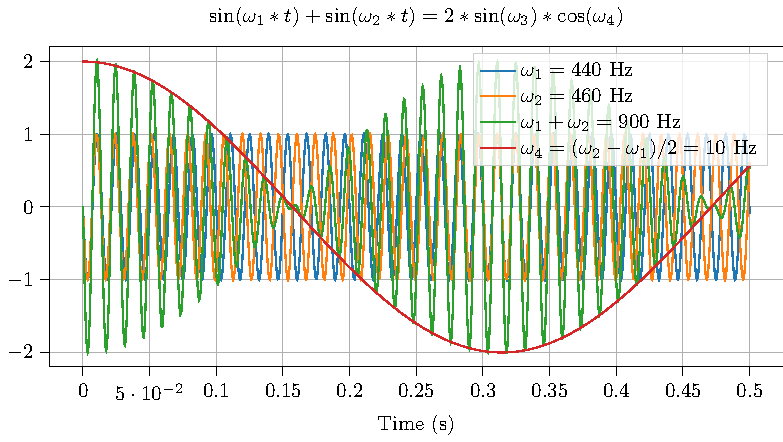
\includegraphics[scale=0.5, trim= {0cm 0cm 0cm 0cm}, clip]{battement/main.pdf}
%	\scalebox{0.3}{\documentclass{standalone}
\usepackage{graphicx}
\usepackage{tikz}
\usepackage{pgfplots}
\usepgfplotslibrary{groupplots}
\pgfplotsset{compat=newest}

\begin{document}
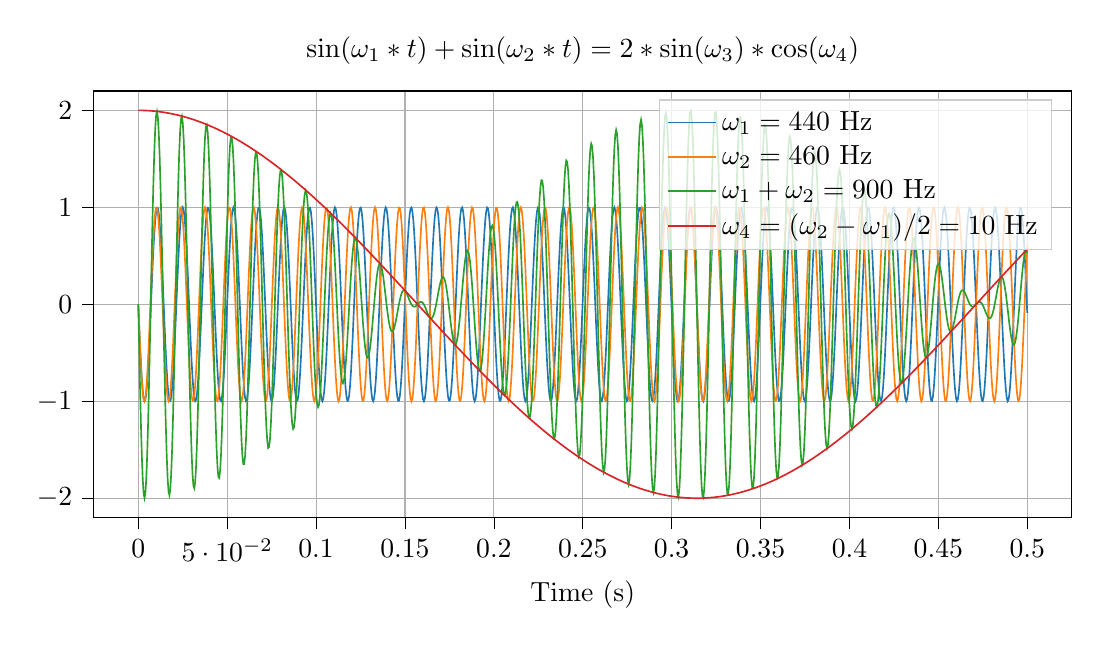
\begin{tikzpicture}

\definecolor{crimson2143940}{RGB}{214,39,40}
\definecolor{darkgray176}{RGB}{176,176,176}
\definecolor{darkorange25512714}{RGB}{255,127,14}
\definecolor{forestgreen4416044}{RGB}{44,160,44}
\definecolor{lightgray204}{RGB}{204,204,204}
\definecolor{steelblue31119180}{RGB}{31,119,180}

\begin{axis}[
width=  14cm,
height= 7cm,
legend cell align={left},
legend style={fill opacity=0.8, draw opacity=1, text opacity=1, draw=lightgray204},
tick align=outside,
tick pos=left,
title={$\sin(\omega_1*t) + \sin(\omega_2*t) = 2*\sin(\omega_3)*\cos(\omega_4)$},
x grid style={darkgray176},
xlabel={Time (s)},
xmajorgrids,
xmin=-0.025, xmax=0.525,
xtick style={color=black},
y grid style={darkgray176},
ymajorgrids,
ymin=-2.19999747578176, ymax=2.19999987979913,
ytick style={color=black}
]
\addplot [semithick, steelblue31119180]
table {%
0 -0
0.0005005005005005 -0.218444530138601
0.001001001001001 -0.426337912960628
0.0015015015015015 -0.613638634920724
0.002002002002002 -0.77129983405971
0.0025025025025025 -0.891706274888888
0.003003003003003 -0.969042173903647
0.0035035035035035 -0.999572109288449
0.004004004004004 -0.981821446518887
0.0045045045045045 -0.916647565075827
0.005005005005005 -0.807198445931199
0.00550550550550551 -0.658760620082286
0.00600600600600601 -0.478503822412767
0.00650650650650651 -0.275134684422264
0.00700700700700701 -0.058476192903904
0.00750750750750751 0.161006772751895
0.00800800800800801 0.372712907478608
0.00850850850850851 0.566416536987634
0.00900900900900901 0.73276153078027
0.00950950950950951 0.86371321509395
0.01001001001001 0.952946457815406
0.0105105105105105 0.996151180368205
0.011011011011011 0.991240539963758
0.0115115115115115 0.938451726749574
0.012012012012012 0.840334507224895
0.0125125125125125 0.701628067291242
0.013013013013013 0.529032103574431
0.0135135135135135 0.330883219596952
0.014014014014014 0.116752257275217
0.0145145145145145 -0.103017986859947
0.015015015015015 -0.317812331827819
0.0155155155155155 -0.517255938876039
0.016016016016016 -0.691715429324997
0.0165165165165165 -0.832764188952155
0.017017017017017 -0.933589384125555
0.0175175175175175 -0.989321030292037
0.018018018018018 -0.997267218395675
0.0185185185185185 -0.95704413749264
0.019019019019019 -0.870594613305622
0.0195195195195195 -0.742094267282164
0.02002002002002 -0.577749828793169
0.0205205205205205 -0.385499342247698
0.021021021021021 -0.174628749499904
0.0215215215215215 0.0446766328968421
0.022022022022022 0.261824077372211
0.0225225225225225 0.46632508748904
0.023023023023023 0.648302005597754
0.0235235235235235 0.798965116204161
0.024024024024024 0.91103720035399
0.0245245245245245 0.979105034520013
0.025025025025025 0.999880856150566
0.0255255255255255 0.972361166762497
0.026026026026026 0.89787520218815
0.0265265265265265 0.780020728802093
0.027027027027027 0.624490266851112
0.0275275275275275 0.438796134520599
0.028028028028028 0.231907593456977
0.0285285285285285 0.0138176220767222
0.029029029029029 -0.204939757940424
0.0295295295295295 -0.413798288232745
0.03003003003003 -0.602669837410364
0.0305305305305305 -0.762431670571117
0.031031031031031 -0.885367088944039
0.0315315315315315 -0.965538156207928
0.032032032032032 -0.999072508332011
0.0325325325325325 -0.984350393660328
0.033033033033033 -0.922082908967032
0.0335335335335335 -0.815277652582069
0.034034034034034 -0.669093453584785
0.0345345345345345 -0.490591193829242
0.035035035035035 -0.288392758412896
0.0355355355355355 -0.0722645877126469
0.036036036036036 0.147354054047896
0.0365365365365365 0.359855308474605
0.037037037037037 0.554975095990888
0.0375375375375375 0.723288883873703
0.038038038038038 0.856666903113788
0.0385385385385385 0.948666826549635
0.039039039039039 0.994844941424193
0.0395395395395395 0.992970786335962
0.04004004004004 0.943134885348039
0.0405405405405405 0.847744375561292
0.041041041041041 0.711406739345383
0.0415415415415415 0.540707257108089
0.042042042042042 0.343890929915843
0.0425425425425425 0.130464235505545
0.043043043043043 -0.0892640466235631
0.0435435435435435 -0.304680762308772
0.044044044044044 -0.505381011504269
0.0445445445445445 -0.681670718124049
0.045045045045045 -0.825034866187806
0.0455455455455455 -0.928548785871232
0.046046046046046 -0.987212623823902
0.0465465465465465 -0.998192842414995
0.047047047047047 -0.960959083187612
0.0475475475475475 -0.877309783843573
0.048048048048048 -0.751285311425932
0.0485485485485486 -0.588972807476425
0.049049049049049 -0.398212171393801
0.0495495495495495 -0.188217383368975
0.05005005005005 0.0308685425214051
0.0505505505505505 0.248463478734064
0.0510510510510511 0.454057314414482
0.0515515515515515 0.637719607055047
0.0520520520520521 0.790579235438302
0.0525525525525526 0.905252886020964
0.0530530530530531 0.976201676323989
0.0535535535535536 0.999998689967533
0.0540540540540541 0.97549450106994
0.0545545545545546 0.903872692972791
0.0550550550550551 0.788592689667305
0.0555555555555556 0.635222661236572
0.0560560560560561 0.451170574192235
0.0565565565565566 0.245326377314864
0.0570570570570571 0.0276326058748024
0.0575575575575576 -0.191395855406851
0.0580580580580581 -0.40117965460015
0.0585585585585586 -0.591585968656091
0.0590590590590591 -0.753417931586155
0.0595595595595596 -0.878858854731102
0.0600600600600601 -0.961849782717742
0.0605605605605606 -0.998382148672956
0.0610610610610611 -0.986691393077808
0.0615615615615616 -0.927342194225901
0.0620620620620621 -0.823201193547033
0.0625625625625626 -0.679298533197478
0.0630630630630631 -0.502584893826608
0.0635635635635636 -0.301595767903226
0.0640640640640641 -0.0860391846249543
0.0645645645645646 0.133673200180593
0.0650650650650651 0.34692900021156
0.0655655655655656 0.543427690383553
0.0660660660660661 0.713678135229817
0.0665665665665666 0.849457022758307
0.0670670670670671 0.944206060830119
0.0675675675675676 0.993348750971409
0.0680680680680681 0.994511439042682
0.0685685685685686 0.947637965738346
0.0690690690690691 0.854992379152255
0.0695695695695696 0.72104957838891
0.0700700700700701 0.552279170272305
0.0705705705705706 0.356832979146981
0.0710710710710711 0.144151303443486
0.0715715715715716 -0.0754930626855624
0.0720720720720721 -0.291491018326465
0.0725725725725726 -0.493409588807807
0.0730730730730731 -0.671495851583309
0.0735735735735736 -0.817148014736221
0.0740740740740741 -0.923330894417233
0.0745745745745746 -0.984915723129615
0.0750750750750751 -0.99892787569141
0.0755755755755756 -0.964690547397058
0.0760760760760761 -0.883857444541383
0.0765765765765766 -0.760332908312263
0.0770770770770771 -0.600083330169054
0.0775775775775776 -0.410848967582785
0.0780780780780781 -0.20177007980251
0.0785785785785786 0.0170545582362964
0.0790790790790791 0.235055439524327
0.0795795795795796 0.441702845546089
0.0800800800800801 0.627015445012837
0.0805805805805806 0.782042404798426
0.0810810810810811 0.899295726509397
0.0815815815815816 0.973111926285815
0.0820820820820821 0.999925588240659
0.0825825825825826 0.978441578560304
0.0830830830830831 0.909697602107147
0.0835835835835836 0.797014079961194
0.0840840840840841 0.645833768878859
0.0845845845845846 0.463458869252066
0.0850850850850851 0.258698319586118
0.0855855855855856 0.0414423136193367
0.0860860860860861 -0.177815408553659
0.0865865865865866 -0.388484421411681
0.0870870870870871 -0.580389144965193
0.0875875875875876 -0.744260338150229
0.0880880880880881 -0.872182814904949
0.0885885885885886 -0.957977757675608
0.0890890890890891 -0.997501162125655
0.0895895895895896 -0.988843997790741
0.0900900900900901 -0.932424416666632
0.0905905905905906 -0.830967555938507
0.0910910910910911 -0.689373910405391
0.0915915915915916 -0.514482632378228
0.0920920920920921 -0.314741191966148
0.0925925925925926 -0.0997973535772359
0.0930930930930931 0.119966823314679
0.0935935935935936 0.333936450784407
0.0940940940940941 0.53177652497869
0.0945945945945946 0.703931119884544
0.0950950950950951 0.842084950651739
0.0955955955955956 0.939565012376703
0.0960960960960961 0.991662894686164
0.0965965965965966 0.995862203918173
0.0970970970970971 0.951960108121263
0.0975975975975976 0.862077134094462
0.0980980980980981 0.730554743258693
0.0985985985985986 0.563745633574649
0.0990990990990991 0.369706896189939
0.0995995995995996 0.157810847737845
0.1001001001001 -0.0617076644196983
0.100600600600601 -0.278245618275137
0.101101101101101 -0.481343956559751
0.101601601601602 -0.661192772448991
0.102102102102102 -0.809105140479652
0.102602602602603 -0.917936706045813
0.103103103103103 -0.982430766769734
0.103603603603604 -0.999472177880756
0.104104104104104 -0.9682378176509
0.104604604604605 -0.890236345216263
0.105105105105105 -0.769235330431052
0.105605605605606 -0.611079275474592
0.106106106106106 -0.423407317997946
0.106606606606607 -0.215284251105665
0.107107107107107 0.00323731762556294
0.107607607607608 0.22160251981763
0.108108108108108 0.429264039794182
0.108608608608609 0.616191563278793
0.109109109109109 0.773356254271065
0.10960960960961 0.893166859254269
0.11011011011011 0.969836374349374
0.110610610610611 0.999661564927678
0.111111111111111 0.981201836531009
0.111611611611612 0.915348817407571
0.112112112112112 0.80528329173892
0.112612612612613 0.656321563737699
0.113113113113113 0.475658673424721
0.113613613613614 0.272020867088327
0.114114114114114 0.0552441085428231
0.114614614614615 -0.164201010374251
0.115115115115115 -0.375715012641764
0.115615615615616 -0.569081504212087
0.116116116116116 -0.734960638775711
0.116616616616617 -0.865340244160536
0.117117117117117 -0.953922820389701
0.117617617617618 -0.996429716901973
0.118118118118118 -0.99080779678984
0.118618618618619 -0.937328605911043
0.119119119119119 -0.838575256879923
0.11961961961962 -0.699317661458378
0.12012012012012 -0.526282137779949
0.120620620620621 -0.327826520669684
0.121121121121121 -0.113536467642572
0.121621621621622 0.106237540488101
0.122122122122122 0.320880140935883
0.122622622622623 0.520023824400814
0.123123123123123 0.694049698891992
0.123623623623624 0.834552094386526
0.124124124124124 0.934744567331659
0.124624624624625 0.989787694458767
0.125125125125125 0.997022823053069
0.125625625625626 0.956100487245104
0.126126126126126 0.868997287654606
0.126626626626627 0.739920419078527
0.127127127127127 0.575104457656851
0.127627627627628 0.382510222953128
0.128128128128128 0.171440260292693
0.128628628628629 -0.0479104839519304
0.129129129129129 -0.264947091175767
0.12962962962963 -0.469186418521172
0.13013013013013 -0.650763447947701
0.130630630630631 -0.800907779090677
0.131131131131131 -0.912367250700597
0.131631631631632 -0.979758229211376
0.132132132132132 -0.999825645056263
0.132632632632633 -0.97160021664827
0.133133133133133 -0.89644526790774
0.133633633633634 -0.777990877991285
0.134134134134134 -0.621958543873479
0.134634634634635 -0.435884824800671
0.135135135135135 -0.228757316939398
0.135635635635636 -0.0105805411049746
0.136136136136136 0.208107288257845
0.136636636636637 0.416743272172005
0.137137137137137 0.605250028519374
0.137637637637638 0.764522442353273
0.138138138138138 0.886867454475721
0.138638638638639 0.966375645934769
0.139139139139139 0.999206670440092
0.13963963963964 0.983774747950007
0.14014014014014 0.920825259854777
0.140640640640641 0.813398746111958
0.141141141141141 0.66668404331767
0.141641641641642 0.487767657330911
0.142142142142142 0.2852914760703
0.142642642642643 0.0690353553885753
0.143143143143143 -0.150555260344562
0.143643643643644 -0.362873866427601
0.144144144144144 -0.557665205430132
0.144644644644645 -0.72552060910809
0.145145145145145 -0.858332448989551
0.145645645645646 -0.949685745092694
0.146146146146146 -0.995168017579154
0.146646646646647 -0.992582415115583
0.147147147147147 -0.942053825573876
0.147647647647648 -0.846022843788855
0.148148148148148 -0.709127887738434
0.148648648648649 -0.537981157083844
0.149149149149149 -0.340849255556211
0.14964964964965 -0.127253903532321
0.15015015015015 0.0924879731123948
0.150650650650651 0.307762563582886
0.151151151151151 0.50817183266114
0.151651651651652 0.684035758969119
0.152152152152152 0.826859892254559
0.152652652652653 0.929745646090486
0.153153153153153 0.987723508332063
0.153653653653654 0.997993074843635
0.154154154154154 0.960058312563293
0.154654654654655 0.875751518527659
0.155155155155155 0.749144817605667
0.155655655655656 0.586353473712805
0.156156156156156 0.395240514823194
0.156656656656657 0.18503693876533
0.157157157157157 -0.0341041556578836
0.157657657657658 -0.251597976193175
0.158158158158158 -0.45693929600125
0.158658658658659 -0.640209869410782
0.159159159159159 -0.792557495739001
0.15965965965966 -0.906623591789985
0.16016016016016 -0.97689862073762
0.160660660660661 -0.999988209728395
0.161161161161161 -0.974777102386849
0.161661661661662 -0.902483027110238
0.162162162162162 -0.786597879245511
0.162662662662663 -0.632719058123979
0.163163163163163 -0.448279105588291
0.163663663663664 -0.242186704813201
0.164164164164164 -0.0243963796314956
0.164664664664665 0.194572321567772
0.165165165165165 0.404142933342279
0.165665665665666 0.594192929865213
0.166166166166166 0.75554265573594
0.166666666666667 0.880398714955599
0.167167167167167 0.962730401818929
0.167667667667668 0.99856099163354
0.168168168168168 0.986159821556413
0.168668668668669 0.926125883799883
0.169169169169169 0.82135889354959
0.16966966966967 0.6769192290505
0.17017017017017 0.499783508932167
0.170670670670671 0.298507612697755
0.171171171171171 0.0828134209139341
0.171671671671672 -0.136880763926695
0.172172172172172 -0.349963434603631
0.172672672672673 -0.546142428399407
0.173173173173173 -0.715942051586933
0.173673673673674 -0.85116076743092
0.174174174174174 -0.945267340793922
0.174674674674675 -0.993716305060761
0.175175175175175 -0.99416751392981
0.175675675675676 -0.946599173441545
0.176176176176176 -0.853308894654388
0.176676676676677 -0.718802716122211
0.177177177177177 -0.549577456528362
0.177677677677678 -0.353806910119517
0.178178178178178 -0.140947042096956
0.178678678678679 0.0787207464720877
0.179179179179179 0.294586223340455
0.17967967967968 0.496222812729121
0.18018018018018 0.673891212135506
0.180680680680681 0.819009812972558
0.181181181181181 0.924569203126185
0.181681681681682 0.985470730433068
0.182182182182182 0.998772774034074
0.182682682682683 0.963832828385315
0.183183183183183 0.882338537089212
0.183683683683684 0.758226177572264
0.184184184184184 0.597490533902706
0.184684684684685 0.407895341131752
0.185185185185185 0.198598287063142
0.185685685685686 -0.0202913156597913
0.186186186186186 -0.238200822151243
0.186686686686687 -0.444604927414067
0.187187187187187 -0.629534051894142
0.187687687687688 -0.784055884792597
0.188188188188188 -0.900706825984025
0.188688688688689 -0.973852487350079
0.189189189189189 -0.999959840857738
0.18968968968969 -0.977767868285435
0.19019019019019 -0.908348469999403
0.190690690690691 -0.795054690809128
0.191191191191191 -0.643358763658748
0.191691691691692 -0.460587793848945
0.192192192192192 -0.255569850576223
0.192692692692693 -0.0382075600159158
0.193193193193193 0.181000204056967
0.193693693693694 0.391465429160683
0.194194194194194 0.583022378512214
0.194694694694695 0.746418608981752
0.195195195195195 0.873761875807826
0.195695695695696 0.958901338009435
0.196196196196196 0.99772465179122
0.196696696696697 0.988356601954301
0.197197197197197 0.931249677164043
0.197697697697698 0.829162214174752
0.198198198198198 0.687025166672885
0.198698698698699 0.511703933972343
0.199199199199199 0.311666753537199
0.1996996996997 0.096575674393019
0.2002002002002 -0.123180132071495
0.200700700700701 -0.33698618223342
0.201201201201201 -0.534515373230497
0.201701701701702 -0.706226795101712
0.202202202202202 -0.843826568815364
0.202702702702703 -0.940668451124918
0.203203203203203 -0.992074856530675
0.203703703703704 -0.995562790580423
0.204204204204204 -0.950963781644468
0.204704704704705 -0.860432018308615
0.205205205205205 -0.728340299338664
0.205705705705706 -0.561068821964867
0.206206206206206 -0.366697010279511
0.206706706706707 -0.154613268826199
0.207207207207207 0.0649384892235648
0.207707707707708 0.281353636043577
0.208208208208208 0.484179046100354
0.208708708708709 0.663617995348241
0.209209209209209 0.811003355401636
0.20970970970971 0.919216226807001
0.21021021021021 0.983029790897723
0.210710710710711 0.999361771751904
0.211211211211211 0.967423314020987
0.211711711711712 0.888757085641624
0.212212212212212 0.767162765021626
0.212712712712713 0.608513511763124
0.213213213213213 0.420472285619506
0.213713713713714 0.212121715839346
0.214214214214214 -0.00647460132321856
0.214714714714715 -0.224758187046209
0.215215215215215 -0.432185667832051
0.215715715715716 -0.61873803379347
0.216216216216216 -0.775404569513328
0.216716716716717 -0.894618083005115
0.217217217217217 -0.970620410664654
0.217717717717718 -0.999740543860924
0.218218218218218 -0.980571943299771
0.218718718718719 -0.914040476652244
0.219219219219219 -0.803359697974112
0.21971971971972 -0.653875628977167
0.22022022022022 -0.472808539413498
0.220720720720721 -0.268904198906909
0.221221221221221 -0.0520114452095001
0.221721721721722 0.167393527128505
0.222222222222222 0.37871318021657
0.222722722722723 0.571740507318468
0.223223223223223 0.737152044197812
0.223723723723724 0.866958204242552
0.224224224224224 0.954889185611622
0.224724724724725 0.996697810600342
0.225225225225225 0.990364669699667
0.225725725725726 0.936195661631705
0.226226226226226 0.836807218054202
0.226726726726727 0.696999926599581
0.227227227227227 0.523526656415593
0.227727727727728 0.324766386037588
0.228228228228228 0.110319488119049
0.228728728728729 -0.109455980719977
0.229229229229229 -0.323944587138933
0.22972972972973 -0.522786259944409
0.23023023023023 -0.696376694642642
0.230730730730731 -0.836331253503914
0.231231231231231 -0.935889954178331
0.231731731731732 -0.990243985400176
0.232232232232232 -0.996767978659163
0.232732732732733 -0.955146816822697
0.233233233233233 -0.867390854692272
0.233733733733734 -0.737738816321798
0.234234234234234 -0.572453059280387
0.234734734734735 -0.3795170948547
0.235235235235235 -0.1682499743482
0.235735735735736 0.0511438328930425
0.236236236236236 0.268067328266814
0.236736736736737 0.472042832361005
0.237237237237237 0.653218070132159
0.237737737737738 0.802842048261143
0.238238238238238 0.913687739207711
0.238738738738739 0.980401155788747
0.239239239239239 0.999759955536376
0.23973973973974 0.970829083918087
0.24024024024024 0.895005938654239
0.240740740740741 0.77595287363934
0.241241241241241 0.61942030261303
0.241741741741742 0.432968946897547
0.242242242242242 0.225604642987289
0.242742742742743 0.00734334924648431
0.243243243243243 -0.211272637558265
0.243743743743744 -0.41968388853639
0.244244244244244 -0.607823876455042
0.244744744744745 -0.766605201746909
0.245245245245245 -0.888358525412222
0.245745745745746 -0.967203007800471
0.246246246246246 -0.999330360609599
0.246746746746747 -0.983188792031561
0.247247247247247 -0.91955796026095
0.247747747747748 -0.811511315017307
0.248248248248248 -0.664267646033207
0.248748748748749 -0.484939008904192
0.249249249249249 -0.282187203800888
0.24974974974975 -0.0658053995565259
0.25025025025025 0.153754888784034
0.250750750750751 0.365888621370717
0.251251251251251 0.560349470397011
0.251751751751752 0.727744730703042
0.252252252252252 0.859988999324201
0.252752752752753 0.950694710689004
0.253253253253253 0.995480664121644
0.253753753753754 0.992183641380502
0.254254254254254 0.940962892837403
0.254754754754755 0.844292445483084
0.255255255255255 0.706841604291891
0.255755755755756 0.535249418881022
0.256256256256256 0.337804009010202
0.256756756756757 0.12404223790601
0.257257257257257 -0.0957109303038598
0.257757757757758 -0.310841139427523
0.258258258258258 -0.510957328048698
0.258758758758759 -0.686393630946465
0.259259259259259 -0.828676252620542
0.25975975975976 -0.930932762340266
0.26026026026026 -0.988224041248096
0.260760760760761 -0.997782848052489
0.261261261261261 -0.959147480285093
0.261761761761762 -0.874184075114395
0.262262262262262 -0.746996472558293
0.262762762762763 -0.583727994816498
0.263263263263263 -0.392264716032056
0.263763763763764 -0.181854554927777
0.264264264264264 0.0373394113741657
0.264764764764765 0.254729836841875
0.265265265265265 0.45981648874867
0.265765765765766 0.642693422205208
0.266266266266266 0.794527449836729
0.266766766766767 0.907984795914497
0.267267267267267 0.977585327006676
0.267767767767768 0.999967249359954
0.268268268268268 0.974049487793236
0.268768768768769 0.901083902997352
0.269269269269269 0.784594825079048
0.26976976976977 0.630208823955663
0.27027027027027 0.445382938905947
0.270770770770771 0.239044494133613
0.271271271271271 0.0211598977079684
0.271771771771772 -0.197746748561537
0.272272272272272 -0.407101976564253
0.272772772772773 -0.596793663782189
0.273273273273273 -0.757659461607638
0.273773773773774 -0.881929348378939
0.274274274274274 -0.963600931262056
0.274774774774775 -0.998729369422429
0.275275275275275 -0.985617914830717
0.275775775775776 -0.924899867340408
0.276276276276276 -0.81950798550325
0.276776776776777 -0.67453283061885
0.277277277277277 -0.496976886180167
0.277777777777778 -0.295416329057033
0.278278278278278 -0.0795867892973255
0.278778778778779 0.140086893127782
0.279279279279279 0.352994201290397
0.27977977977978 0.54885144270452
0.28028028028028 0.718198464690304
0.280780780780781 0.852855591723469
0.281281281281281 0.946318714116965
0.281781781781782 0.994073444751955
0.282282282282282 0.993813169689998
0.282782782782783 0.945550460546047
0.283283283283283 0.851616467263533
0.283783783783784 0.716548320621282
0.284284284284284 0.546869983073718
0.284784784784785 0.350777133106148
0.285285285285285 0.137741303589791
0.285785785785786 -0.0819476052453016
0.286286286286286 -0.29767834101633
0.286786786786787 -0.499030836109858
0.287287287287287 -0.676279510137405
0.287787787787788 -0.820863027778945
0.288288288288288 -0.925797822116091
0.288788788788789 -0.986015409754074
0.289289289289289 -0.998607204985511
0.28978978978979 -0.962965008161803
0.29029029029029 -0.880810382506057
0.290790790790791 -0.756111500430184
0.291291291291291 -0.594891475784477
0.291791791791792 -0.404937439834434
0.292292292292292 -0.195424412963493
0.292792792792793 0.0235278604251458
0.293293293293293 0.241343708373304
0.293793793793794 0.447502349709973
0.294294294294294 0.632046061099383
0.294794794794795 0.786061147682855
0.295295295295295 0.902108485823358
0.295795795795796 0.974582842194022
0.296296296296296 0.999983613642827
0.296796796796797 0.977083910756065
0.297297297297297 0.906989818170002
0.297797797797798 0.793086969282863
0.298298298298298 0.640877015876103
0.298798798798799 0.457711891369296
0.299299299299299 0.252438703129668
0.2997997997998 0.0349724059875831
0.3003003003003 -0.184183102632381
0.300800800800801 -0.394442334253005
0.301301301301301 -0.58564950183728
0.301801801801802 -0.748569057157485
0.302302302302302 -0.875331779465307
0.302802802802803 -0.959814868814759
0.303303303303303 -0.997937685050142
0.303803803803804 -0.98785884789075
0.304304304304304 -0.930065177929349
0.304804804804805 -0.827348182581305
0.305305305305305 -0.684669222742907
0.305805805805806 -0.508919872779817
0.306306306306306 -0.308589048761876
0.306806806806807 -0.0933529830713065
0.307307307307307 0.126392149869379
0.307807807807808 0.340032381982024
0.308308308308308 0.537248619626043
0.308808808808809 0.70851506888347
0.309309309309309 0.845559343463186
0.30980980980981 0.941762031429898
0.31031031031031 0.992476421179826
0.310810810810811 0.995252943492881
0.311311311311311 0.949957488826773
0.311811811811812 0.858777884977644
0.312312312312312 0.726118222228133
0.312812812812813 0.558386130211971
0.313313313313313 0.36368328129169
0.313813813813814 0.151414069528407
0.314314314314314 -0.0681686334556575
0.314814814814815 -0.284458705154773
0.315315315315315 -0.48700906132212
0.315815815815816 -0.666036263363107
0.316316316316316 -0.81289307080337
0.316816816816817 -0.920486113949697
0.317317317317317 -0.983618512624921
0.317817817817818 -0.999240892058978
0.318318318318318 -0.96659867155011
0.318818818818819 -0.887268511668
0.319319319319319 -0.765082159552408
0.31981981981982 -0.605941370676186
0.32032032032032 -0.417532846585175
0.320820820820821 -0.2089569574838
0.321321321321321 0.00971181716541509
0.321821821821822 0.227911498752153
0.322322322322322 0.435102766454829
0.322822822822823 0.621278019777077
0.323323323323323 0.777444758319609
0.323823823823824 0.896059930932228
0.324324324324324 0.971394274632597
0.324824824824825 0.999809045260468
0.325325325325325 0.979931773426612
0.325825825825826 0.912722556521593
0.326326326326326 0.801427684796534
0.326826826826827 0.651422841434688
0.327327327327327 0.469953450249242
0.327827827827828 0.265784712541498
0.328328328328328 0.0487782367830935
0.328828828828829 -0.170584289556245
0.329329329329329 -0.381707378781516
0.32982982982983 -0.574393518439758
0.33033033033033 -0.739335724080096
0.330830830830831 -0.868567078383351
0.331331331331331 -0.955845543353417
0.331831831831832 -0.996955458653623
0.332332332332332 -0.989911163337326
0.332832832832833 -0.935052905785104
0.333333333333333 -0.835030409277249
0.333833833833834 -0.694674887005309
0.334334334334334 -0.520765688359477
0.334834834834835 -0.321702847771629
0.335335335335335 -0.107101352419387
0.335835835835836 0.112673273825489
0.336336336336336 0.327005638320781
0.336836836836837 0.525543216555815
0.337337337337337 0.698696392189426
0.337837837837838 0.838101647658283
0.338338338338338 0.937025532661625
0.338838838838839 0.990689898334217
0.339339339339339 0.996502687884788
0.33983983983984 0.954183136220123
0.34034034034034 0.865775331254439
0.340840840840841 0.735549481875734
0.341341341341341 0.569795661451085
0.341841841841842 0.37651998932115
0.342342342342342 0.165057925101439
0.342842842842843 -0.0543766458338319
0.343343343343343 -0.271184755944454
0.343843843843844 -0.474894299072585
0.344344344344344 -0.655665846426059
0.344844844844845 -0.804767903443939
0.345345345345345 -0.914998652036276
0.345845845845846 -0.981033807514093
0.346346346346346 -0.999683788279348
0.346846846846847 -0.97004777665361
0.347347347347347 -0.893557229512193
0.347847847847848 -0.77390673710507
0.348348348348348 -0.616875569671183
0.348848848848849 -0.430048531370369
0.349349349349349 -0.222449604641467
0.34984984984985 -0.004106080427837
0.35035035035035 0.214435772668033
0.350850850850851 0.422620106507486
0.351351351351351 0.610391354242807
0.351851851851852 0.76867992692418
0.352352352352352 0.889840286126736
0.352852852852853 0.968020233134075
0.353353353353353 0.999443577544229
0.353853853853854 0.982592532045958
0.354354354354354 0.918281023467176
0.354854854854855 0.809615379078861
0.355355355355355 0.661844287055851
0.355855855855856 0.482105278194034
0.356356356356356 0.279079974138212
0.356856856856857 0.062574754067235
0.357357357357357 -0.156952905833371
0.357857857857858 -0.36889954170854
0.358358358358358 -0.56302786275974
0.358858858858859 -0.729961225349197
0.359359359359359 -0.861636536756692
0.35985985985986 -0.951693712764337
0.36036036036036 -0.99578287777505
0.360860860860861 -0.99177446930997
0.361361361361361 -0.939862098571864
0.361861861861862 -0.842553198778989
0.362362362362362 -0.704547912966608
0.362862862862863 -0.532512071128978
0.363363363363363 -0.334755222192772
0.363863863863864 -0.12082927228568
0.364364364364364 0.0989328844206014
0.364864864864865 0.313916457578404
0.365365365365365 0.513737468474242
0.365865865865866 0.688744309344991
0.366366366366366 0.830483928249869
0.366866866866867 0.932110122179299
0.367367367367367 0.988714217326283
0.367867867867868 0.997562164244791
0.368368368368368 0.958226595898763
0.368868868868869 0.872607470030958
0.369369369369369 0.744840298798967
0.36986986986987 0.581096398303223
0.37037037037037 0.389284806207502
0.370870870870871 0.17867026520849
0.371371371371371 -0.0405742757640172
0.371871871871872 -0.257859027857472
0.372372372372372 -0.462688862503003
0.372872872872873 -0.64517023941002
0.373373373373373 -0.796489077085881
0.373873873873874 -0.909336484128754
0.374374374374374 -0.978261787934311
0.374874874874875 -0.999935809081881
0.375375375375375 -0.973311664914688
0.375875875875876 -0.899675335297295
0.376376376376376 -0.782583548160402
0.376876876876877 -0.627691985039502
0.377377377377377 -0.442482104497804
0.377877877877878 -0.235899778207308
0.378378378378378 -0.0179231940233625
0.378878878878879 0.200919103119402
0.379379379379379 0.410056753254609
0.37987987987988 0.599388143150636
0.38038038038038 0.759768327016591
0.380880880880881 0.883450738959702
0.381381381381381 0.964461361923771
0.381881881881882 0.998887280274979
0.382382382382382 0.985065678580045
0.382882882882883 0.923664157696462
0.383383383383383 0.817648488805987
0.383883883883884 0.672139362912557
0.384384384384384 0.494165054984755
0.384884884884885 0.292321949378481
0.385385385385385 0.0763593235910542
0.385885885885886 -0.143291554182834
0.386386386386386 -0.356021268508698
0.386886886886887 -0.551554704907716
0.387387387387387 -0.720447350892147
0.387887887887888 -0.854541477873741
0.388388388388388 -0.947360169780591
0.388888888888889 -0.994420166302082
0.389389389389389 -0.993448410036866
0.38988988988989 -0.944491838042627
0.39039039039039 -0.849915114716755
0.390890890890891 -0.714286415512751
0.391391391391391 -0.54415677828333
0.391891891891892 -0.347743679859751
0.392392392392392 -0.134534121518933
0.392892892892893 0.0851736051868483
0.393393393393393 0.300767338947932
0.393893893893894 0.501833629521256
0.394394394394394 0.678660720559007
0.394894894894895 0.822707639733232
0.395395395395395 0.927016738510712
0.395895895895896 0.986549755384258
0.396396396396396 0.998431170280922
0.396896896896897 0.962087095821507
0.397397397397397 0.879272996807371
0.397897897897898 0.753988899048402
0.398398398398398 0.592286183053152
0.398898898898899 0.401975294690298
0.399399399399399 0.192248490766593
0.3998998998999 -0.0267641586125877
0.4004004004004 -0.244484065252272
0.400900900900901 -0.450395082068096
0.401401401401401 -0.634551446302113
0.401901901901902 -0.788058172453481
0.402402402402402 -0.903500691337645
0.402902902902903 -0.975302983163336
0.403403403403403 -0.999996906346782
0.403903903903904 -0.976389713140234
0.404404404404404 -0.905621660857957
0.404904904904905 -0.791110936004614
0.405405405405405 -0.638388551540286
0.405905905905906 -0.454831191953247
0.406406406406406 -0.249304910061671
0.406906906906907 -0.0317368854396066
0.407407407407407 0.187364070922264
0.407907907907908 0.397415105489948
0.408408408408408 0.588270487407475
0.408908908908909 0.750711660140247
0.409409409409409 0.876892509424388
0.40990990990991 0.960718340517556
0.41041041041041 0.99814025966978
0.410910910910911 0.987350740816676
0.411411411411411 0.928870931376412
0.411911911911912 0.825525480169727
0.412412412412412 0.682306103306343
0.412912912912913 0.506130477978348
0.413413413413413 0.30550810989525
0.413913913913914 0.0901293133867679
0.414414414414414 -0.129602843045572
0.414914914914915 -0.343075018105282
0.415415415415415 -0.53997623552019
0.415915915915916 -0.710795917248176
0.416416416416416 -0.847283256435243
0.416916916916917 -0.942845741830648
0.417417417417417 -0.992867584425114
0.417917917917918 -0.994932665902822
0.418418418418418 -0.948941240214382
0.418918918918919 -0.857114751437281
0.419419419419419 -0.723888535215022
0.41991991991992 -0.555697586431222
0.42042042042042 -0.360665740811091
0.420920920920921 -0.148213283372878
0.421421421421421 0.0713980632632197
0.421921921921922 0.287560793066768
0.422422422422422 0.489833972565774
0.422922922922923 0.668447551149504
0.423423423423423 0.814774266880193
0.423923923923924 0.921746354165141
0.424424424424424 0.984196925781385
0.424924924924925 0.999109540068827
0.425425425425425 0.965763898880737
0.425925925925926 0.885770638895992
0.426426426426426 0.762993535828731
0.426926926926927 0.60336287917046
0.427427427427427 0.41458903170107
0.427927927927928 0.205790009206472
0.428428428428428 -0.0129489312253119
0.428928928928929 -0.231062421887959
0.429429429429429 -0.438015305090592
0.42992992992993 -0.623811494609946
0.43043043043043 -0.77947679930826
0.430930930930931 -0.89749238792468
0.431431431431431 -0.972157958142904
0.431931931931932 -0.999867068408398
0.432432432432432 -0.979281333620668
0.432932932932933 -0.911395070827751
0.433433433433433 -0.799487272454139
0.433933933933934 -0.648963226816139
0.434434434434434 -0.46709343585398
0.434934934934935 -0.26266244068509
0.435435435435435 -0.0455445171484309
0.435935935935936 0.173773264217538
0.436436436436436 0.384697576956558
0.436936936936937 0.57704050977173
0.437437437437437 0.741511655537028
0.437937937937938 0.870166849721557
0.438438438438438 0.956791883592215
0.438938938938939 0.9972026583616
0.439439439439439 0.989447282455677
0.43993993993994 0.93390035034759
0.44044044044044 0.833244849170432
0.440940940940941 0.692342567042561
0.441441441441441 0.517999262547274
0.441941941941942 0.318635937978517
0.442442442442442 0.103882094270441
0.442942942942943 -0.1158893860866
0.443443443443443 -0.33006326240089
0.443943943943944 -0.528294665341383
0.444444444444444 -0.701008767221352
0.444944944944945 -0.839863258295472
0.445445445445445 -0.938151290880393
0.445945945945946 -0.991125428587609
0.446446446446446 -0.996226953510265
0.446946946946947 -0.953209455537
0.447447447447447 -0.864150734272215
0.447947947947948 -0.733352438685074
0.448448448448448 -0.567132292019214
0.448948948948949 -0.373518937762903
0.449449449449449 -0.161864146005884
0.44994994994995 0.0576088888936655
0.45045045045045 0.274299341537319
0.450950950950951 0.477740788771825
0.451451451451451 0.658106751176091
0.451951951951952 0.806685324455581
0.452452452452452 0.916299975447605
0.452952952952953 0.981656177757065
0.453453453453453 0.999597144083432
0.453953953953954 0.96925630304315
0.454454454454454 0.892099155664423
0.454954954954955 0.771852489832499
0.455455455455455 0.614324371717379
0.455955955955956 0.42712360882585
0.456456456456456 0.219292234967579
0.456956956956957 0.000868768576428519
0.457457457457457 -0.217596660436666
0.457957957957958 -0.425551895313037
0.458458458458458 -0.612952434974787
0.458958958958959 -0.770746596141443
0.459459459459459 -0.89131272109004
0.45995995995996 -0.968827313370866
0.46046046046046 -0.99954632005744
0.460960960960961 -0.981985974242154
0.461461461461461 -0.916994462856072
0.461961961961962 -0.807710958166542
0.462462462462462 -0.659413991782977
0.462962962962963 -0.479266494898652
0.463463463463463 -0.275969819646849
0.463963963963964 -0.0593434527787408
0.464464464464464 0.160149277976581
0.464964964964965 0.371906595885923
0.465465465465465 0.565700354448096
0.465965965965966 0.732170069817118
0.466466466466466 0.863275044020369
0.466966966966967 0.952682740848921
0.467467467467467 0.996074655372095
0.467967967967968 0.991354903192207
0.468468468468468 0.938751454313892
0.468968968968969 0.840805121904317
0.469469469469469 0.702246837801039
0.46996996996997 0.529769142515727
0.47047047047047 0.331702927055924
0.470970970970971 0.117615040344022
0.471471471471471 -0.102153801695683
0.471971971971972 -0.316988485805431
0.472472472472472 -0.516512224801245
0.472972972972973 -0.691087769528995
0.473473473473473 -0.832282900197617
0.473973973973974 -0.933277713268535
0.474474474474474 -0.989194031429465
0.474974974974975 -0.997331025733359
0.475475475475475 -0.957295669055402
0.475975975975976 -0.871021719800586
0.476476476476476 -0.742676318925001
0.476976976976977 -0.578458711752719
0.477477477477477 -0.386300816579741
0.477977977977978 -0.175484102979657
0.478478478478478 0.043808714925142
0.478978978978979 0.260985516445252
0.479479479479479 0.465556387161057
0.47997997997998 0.647640295067623
0.48048048048048 0.79844235692809
0.480980980980981 0.910678642266716
0.481481481481481 0.978927996431035
0.481981981981982 0.999893889223676
0.482482482482482 0.972563641483764
0.482982982982983 0.898257338772249
0.483483483483483 0.780564069568289
0.483983983983984 0.625168567752648
0.484484484484485 0.439576632765279
0.484984984984985 0.232752589991634
0.485485485485485 0.014686302499151
0.485985985985986 -0.204089351994246
0.486486486486486 -0.413007232446448
0.486986986986987 -0.60197634077981
0.487487487487487 -0.761869229861356
0.487987987987988 -0.884962870753319
0.488488488488488 -0.965311684786518
0.488988988988989 -0.999034722536245
0.48948948948949 -0.98450311859197
0.48998998998999 -0.922418767818557
0.49049049049049 -0.815780422945812
0.490990990990991 -0.669738851015778
0.491491491491491 -0.491348044814596
0.491991991991992 -0.289224506091981
0.492492492492492 -0.0731310576197204
0.492992992992993 0.146494713506107
0.493493493493493 0.359044604534066
0.493993993993994 0.55425218667811
0.494494494494495 0.722688686623603
0.494994994994995 0.856218408213248
0.495495495495495 0.948391696870081
0.495995995995996 0.994756466077408
0.496496496496497 0.993073238793185
0.496996996996997 0.943423317025899
0.497497497497497 0.848204854844658
0.497997997997998 0.712017024501975
0.498498498498498 0.541437870592354
0.498998998998999 0.344706582171616
0.4994994994995 0.131325529496463
0.5 -0.0883987124875315
};

\addplot [semithick, darkorange25512714]
table {%
0 -0
0.0005005005005005 -0.228201684929414
0.001001001001001 -0.444360656632758
0.0015015015015015 -0.637069722791224
0.002002002002002 -0.796159195041084
0.0025025025025025 -0.913233566170439
0.003003003003003 -0.982114559809117
0.0035035035035035 -0.999167171888789
0.004004004004004 -0.963491497936384
0.0045045045045045 -0.87697022304552
0.005005005005005 -0.744169268373998
0.00550550550550551 -0.57209683727383
0.00600600600600601 -0.369833576728378
0.00650650650650651 -0.148053371304586
0.00700700700700701 0.0815399416049184
0.00750750750750751 0.306830209453549
0.00800800800800801 0.515928361005198
0.00850850850850851 0.697799819210108
0.00900900900900901 0.842846820511688
0.00950950950950951 0.943414910292228
0.01001001001001 0.994196885560238
0.0105105105105105 0.992512867920451
0.011011011011011 0.938451726749574
0.0115115115115115 0.834866389360552
0.012012012012012 0.687223285648449
0.0125125125125125 0.503313872360664
0.013013013013013 0.292843460500861
0.0135135135135135 0.0669190443639517
0.014014014014014 -0.162536839390679
0.0145145145145145 -0.383415290660271
0.015015015015015 -0.58406005963545
0.0155155155155155 -0.753882673168757
0.016016016016016 -0.883921212180955
0.0165165165165165 -0.967313252171779
0.017017017017017 -0.999658008706807
0.0175175175175175 -0.979248576653244
0.018018018018018 -0.90716200738082
0.0185185185185185 -0.787202470352473
0.019019019019019 -0.62570049859477
0.0195195195195195 -0.431178912313552
0.02002002002002 -0.213903050612645
0.0205205205205205 0.0146609534063455
0.021021021021021 0.24245126612876
0.0215215215215215 0.457446883359822
0.022022022022022 0.648302005597754
0.0225225225225225 0.804944781245367
0.023023023023023 0.91910882074185
0.0235235235235235 0.984769432425477
0.024024024024024 0.998461558985219
0.0245245245245245 0.95946263628372
0.025025025025025 0.86983072468265
0.0255255255255255 0.734295900595118
0.026026026026026 0.560010639775794
0.0265265265265265 0.35617236518072
0.027027027027027 0.133538078390339
0.0275275275275275 -0.0961433114190772
0.028028028028028 -0.320751003685976
0.0285285285285285 -0.528431948214095
0.029029029029029 -0.708226357137518
0.0295295295295295 -0.850646077435003
0.03003003003003 -0.948175301982642
0.0305305305305305 -0.995667195502899
0.031031031031031 -0.990615504571727
0.0315315315315315 -0.933286818216327
0.032032032032032 -0.826706499416023
0.0325325325325325 -0.676499029932432
0.033033033033033 -0.490591193829242
0.0335335335335335 -0.27879376335102
0.034034034034034 -0.0522837625326996
0.0345345345345345 0.176985369353197
0.035035035035035 0.396914587517641
0.0355355355355355 0.595897735304917
0.036036036036036 0.763434027033438
0.0365365365365365 0.890682197938346
0.037037037037037 0.970927077484317
0.0375375375375375 0.999933963931392
0.038038038038038 0.976172099015573
0.0385385385385385 0.900895449485558
0.039039039039039 0.77807653247324
0.0395395395395395 0.614196776881189
0.04004004004004 0.417904483885456
0.0405405405405405 0.199558436742914
0.041041041041041 -0.0293187553658944
0.0415415415415415 -0.256648731190449
0.042042042042042 -0.470434779543487
0.0425425425425425 -0.659394932577816
0.043043043043043 -0.813557340458706
0.0435435435435435 -0.924786508179081
0.044044044044044 -0.987212623823902
0.0445445445445445 -0.997541321671194
0.045045045045045 -0.955227533238171
0.0455455455455455 -0.862504251763974
0.046046046046046 -0.724264692162938
0.0465465465465465 -0.547804065131207
0.047047047047047 -0.342434592564476
0.0475475475475475 -0.118994080784272
0.048048048048048 0.110726014737517
0.0485485485485486 0.334602850852341
0.049049049049049 0.540821946277441
0.0495495495495495 0.718500658193111
0.05005005005005 0.858262483640398
0.0505505505505505 0.952731878550315
0.0510510510510511 0.996923481697804
0.0515515515515515 0.988505203362007
0.0520520520520521 0.927921294915947
0.0525525525525526 0.818368904688109
0.0530530530530531 0.665629357295592
0.0535535535535536 0.477763060215644
0.0540540540540541 0.264684138058165
0.0545545545545546 0.0376372420397167
0.0550550550550551 -0.191395855406851
0.0555555555555556 -0.410328565557691
0.0560560560560561 -0.607607319713408
0.0565565565565566 -0.772821276855755
0.0570570570570571 -0.897251727009281
0.0575575575575576 -0.974332197063796
0.0580580580580581 -0.99999497824456
0.0585585585585586 -0.972885788200682
0.0590590590590591 -0.894435239513269
0.0595595595595596 -0.768783343070334
0.0600600600600601 -0.602561030434196
0.0605605605605606 -0.404540224754641
0.0610610610610611 -0.185170926768218
0.0615615615615616 0.0439702551092697
0.0620620620620621 0.270791028296866
0.0625625625625626 0.48332155336916
0.0630630630630631 0.670346119250111
0.0635635635635636 0.821995021367521
0.0640640640640641 0.930265408034228
0.0645645645645646 0.989443608827922
0.0650650650650651 0.996406657756421
0.0655655655655656 0.950787099156765
0.0660660660660661 0.854992379152255
0.0665665665665666 0.714077799336935
0.0670670670670671 0.535479737205619
0.0675675675675676 0.328623211884015
0.0680680680680681 0.104424504792933
0.0685685685685686 -0.1252849169337
0.0690690690690691 -0.348382773427359
0.0695695695695696 -0.553095691901887
0.0700700700700701 -0.728620513863415
0.0705705705705706 -0.865694401942469
0.0710710710710711 -0.957083660535847
0.0715715715715716 -0.997965474099819
0.0720720720720721 -0.986182417911312
0.0725725725725726 -0.922356310195066
0.0730730730730731 -0.809855397385371
0.0735735735735736 -0.654616604229556
0.0740740740740741 -0.464832228992703
0.0745745745745746 -0.250517617558308
0.0750750750750751 -0.0229826312293702
0.0755755755755756 0.205765199944073
0.0760760760760761 0.423654341377358
0.0765765765765766 0.619186295825952
0.0770770770770771 0.782042404798426
0.0775775775775776 0.903628387239943
0.0780780780780781 0.977527878962373
0.0785785785785786 0.999841038530972
0.0790790790790791 0.969390350617862
0.0795795795795796 0.887782766119076
0.0800800800800801 0.759324899762264
0.0805805805805806 0.590795760416915
0.0810810810810811 0.39108900763685
0.0815815815815816 0.170743613357295
0.0820820820820821 -0.0586123032217881
0.0825825825825826 -0.284875117489031
0.0830830830830831 -0.496104434758988
0.0835835835835836 -0.681153211601154
0.0840840840840841 -0.830256010249212
0.0845845845845846 -0.935544342589788
0.0850850850850851 -0.991461907875921
0.0855855855855856 -0.995057811142706
0.0860860860860861 -0.946142288533475
0.0865865865865866 -0.847296721562867
0.0870870870870871 -0.703737411841732
0.0875875875875876 -0.52304030517625
0.0880880880880881 -0.314741191966148
0.0885885885885886 -0.0898324822210656
0.0890890890890891 0.139816888497258
0.0895895895895896 0.362087809346314
0.0900900900900901 0.565250546783136
0.0905905905905906 0.738583748833769
0.0910910910910911 0.872940234812427
0.0915915915915916 0.961229712501482
0.0920920920920921 0.998792948727358
0.0925925925925926 0.983647647514236
0.0930930930930931 0.916593060275567
0.0935935935935936 0.801167807529676
0.0940940940940941 0.643463137981833
0.0945945945945946 0.451801479708597
0.0950950950950951 0.236297247017358
0.0955955955955956 0.00832308018509758
0.0960960960960961 -0.220090314200891
0.0965965965965966 -0.436889050533076
0.0970970970970971 -0.630632174682522
0.0975975975975976 -0.791095428732911
0.0980980980980981 -0.909810807934654
0.0985985985985986 -0.980513436251907
0.0990990990990991 -0.999472177880756
0.0995995995995996 -0.965686537629265
0.1001001001001 -0.880939459286102
0.100600600600601 -0.749703235689726
0.101101101101101 -0.578903495834204
0.101601601601602 -0.377553723939885
0.102102102102102 -0.156279597734818
0.102602602602603 0.0732417523204424
0.103103103103103 0.298897971320064
0.103603603603604 0.508780675967354
0.104104104104104 0.691813886591244
0.104604604604605 0.838338531362049
0.105105105105105 0.940622177111829
0.105605605605606 0.993267087124211
0.106106106106106 0.993495071771514
0.106606606606607 0.941294099794068
0.107107107107107 0.839418933216708
0.107607607607608 0.693245752396426
0.108108108108108 0.510488442962523
0.108608608608609 0.30079151682193
0.109109109109109 0.0752211496984554
0.10960960960961 -0.154318805706699
0.11011011011011 -0.375715012641764
0.110610610610611 -0.577283898173068
0.111111111111111 -0.748388221455954
0.111611611611612 -0.879998424721498
0.112112112112112 -0.965169143232174
0.112612612612613 -0.999405727710523
0.113113113113113 -0.980901437032615
0.113613613613614 -0.910632783997446
0.114114114114114 -0.792308002562827
0.114614614614615 -0.632171356046944
0.115115115115115 -0.438673613389443
0.115615615615616 -0.222026083176579
0.116116116116116 0.00633825994776733
0.116616616616617 0.234368118920845
0.117117117117117 0.450029848156536
0.117617617617618 0.641942495932995
0.118118118118118 0.799978402665501
0.118618618618619 0.915797660150519
0.119119119119119 0.983288227171613
0.11961961961962 0.998888475582392
0.12012012012012 0.961775145388411
0.120620620620621 0.873906790018095
0.121121121121121 0.739920419078527
0.121621621621622 0.566886792989062
0.122122122122122 0.363937283142091
0.122622622622623 0.141781989014827
0.123123123123123 -0.0878554577304478
0.123623623623624 -0.312856575505933
0.124124124124124 -0.521347552171482
0.124624624624625 -0.702325852653871
0.125125125125125 -0.846240847326839
0.125625625625626 -0.945497820093883
0.126126126126126 -0.994858758540297
0.126626626626627 -0.991718775561651
0.127127127127127 -0.936243575081468
0.127627627627628 -0.831360707484606
0.128128128128128 -0.682605076236785
0.128628628628629 -0.497826848651333
0.129129129129129 -0.286777185005267
0.12962962962963 -0.0605936480056157
0.13013013013013 0.168787551300876
0.130630630630631 0.389261454076756
0.131131131131131 0.589193159441351
0.131631631631632 0.758031824208516
0.132132132132132 0.886867454475721
0.132632632632633 0.968901105927174
0.133133133133133 0.999803679329345
0.133633633633634 0.977944376778421
0.134134134134134 0.904476762552526
0.134634634634635 0.783277886945134
0.135135135135135 0.62074368565107
0.135635635635636 0.425451451937138
0.136136136136136 0.207707193695517
0.136636636636637 -0.0209982376392991
0.137137137137137 -0.248595545016905
0.137637637637638 -0.463073909566188
0.138138138138138 -0.653114828366081
0.138638638638639 -0.808689417155578
0.139139139139139 -0.921587656983077
0.13963963963964 -0.985851655266017
0.14014014014014 -0.99809005710567
0.140640640640641 -0.957657014669034
0.141141141141141 -0.866686270023224
0.141641641641642 -0.729978552795065
0.142142142142142 -0.554748234933131
0.142642642642643 -0.35024261216694
0.143143143143143 -0.127253903532321
0.143643643643644 0.102450278161206
0.144144144144144 0.32674792957338
0.144644644644645 0.533802362057156
0.145145145145145 0.712686850188248
0.145645645645646 0.853961259500406
0.146146146146146 0.950170223491605
0.146646646646647 0.996236579986279
0.147147147147147 0.989729304337062
0.147647647647648 0.930991800031749
0.148148148148148 0.823123776523339
0.148648648648649 0.671817670630478
0.149149149149149 0.485058243917013
0.14964964964965 0.272701208968344
0.15015015015015 0.0459531213987264
0.150650650650651 -0.183220015149017
0.151151151151151 -0.40272422177455
0.151651651651652 -0.60097577063148
0.152152152152152 -0.767512484149792
0.152652652652653 -0.893545847542078
0.153153153153153 -0.972424798382044
0.153653653653654 -0.999986718042089
0.154154154154154 -0.974777102386849
0.154654654654655 -0.898126319209046
0.155155155155155 -0.774079401746063
0.155655655655656 -0.60918258323033
0.156156156156156 -0.412137837522783
0.156656656656657 -0.193343656492567
0.157157157157157 0.0356537016524289
0.157657657657658 0.262769534231182
0.158158158158158 0.476018430874416
0.158658658658659 0.664146770431875
0.159159159159159 0.817226599726097
0.15965965965966 0.927179553842951
0.16016016016016 0.988203169513157
0.160660660660661 0.99707709407472
0.161161161161161 0.953333030684356
0.161661661661662 0.859279451389131
0.162162162162162 0.719879773894258
0.162662662662663 0.542490430911424
0.163163163163163 0.336472654753913
0.163663663663664 0.112698464173466
0.164164164164164 -0.117023076381541
0.164664664664665 -0.340569047504923
0.165165165165165 -0.546142428399407
0.165665665665666 -0.722894652045051
0.166166166166166 -0.861498108340745
0.166666666666667 -0.954638382948014
0.167167167167167 -0.997400255292403
0.167667667667668 -0.987527085744741
0.168168168168168 -0.925539903540782
0.168668668668669 -0.814709910903251
0.169169169169169 -0.660885854385445
0.16966966966967 -0.472185373436354
0.17017017017017 -0.258566614414084
0.170670670670671 -0.0313027169337532
0.171171171171171 0.197613094919355
0.171671671671672 0.41610042184448
0.172172172172172 0.612629199011
0.172672672672673 0.776828163363522
0.173173173173173 0.900032168365872
0.173673673673674 0.9757394631611
0.174174174174174 0.999954804503651
0.174674674674675 0.971400294679705
0.175175175175175 0.891582819027242
0.175675675675676 0.764714524226968
0.176176176176176 0.597490533902706
0.176676676676677 0.398735631975811
0.177177177177177 0.178938559083388
0.177677677677678 -0.0503015017203121
0.178178178178178 -0.276887039792321
0.178678678678679 -0.488860629590303
0.179179179179179 -0.675035950758078
0.17967967967968 -0.825588115266081
0.18018018018018 -0.932572148723356
0.180680680680681 -0.99034226444304
0.181181181181181 -0.995849804231114
0.181681681681682 -0.948804122896817
0.182182182182182 -0.851687926249304
0.182682682682683 -0.709626253160196
0.183183183183183 -0.530116015801536
0.183683683683684 -0.322630370825634
0.184184184184184 -0.0981187997042617
0.184684684684685 0.131570719894063
0.185185185185185 0.354316958380675
0.185685685685686 0.558365098637967
0.186186186186186 0.732947064005146
0.186686686686687 0.868849773763708
0.187187187187187 0.958901338009435
0.187687687687688 0.998349534320718
0.188188188188188 0.985112593162821
0.188688688688689 0.91988905752154
0.189189189189189 0.806120919227745
0.18968968968969 0.649811977351381
0.19019019019019 0.459211004298599
0.190690690690691 0.244376439645762
0.191191191191191 0.0166455837899513
0.191691691691692 -0.211963696745901
0.192192192192192 -0.42938717900404
0.192692692692693 -0.62415093961598
0.193193193193193 -0.785976859396891
0.193693693693694 -0.906325022679319
0.194194194194194 -0.978844387760225
0.194694694694695 -0.999707945574008
0.195195195195195 -0.967814679519053
0.195695695695696 -0.884847668565868
0.196196196196196 -0.755185267416117
0.196696696696697 -0.585670050933909
0.197197197197197 -0.385247716168693
0.197697697697698 -0.164494997917264
0.198198198198198 0.0649384892235648
0.198698698698699 0.290945027070414
0.199199199199199 0.501597745217623
0.1996996996997 0.685780028659803
0.2002002002002 0.833772166425064
0.200700700700701 0.937764282458485
0.201201201201201 0.992268480246285
0.201701701701702 0.994408451387072
0.202202202202202 0.94407126481827
0.202702702702703 0.843913326440833
0.203203203203203 0.699220194639519
0.203703703703704 0.517627649547181
0.204204204204204 0.308718735851714
0.204704704704705 0.0835180440980739
0.205205205205205 -0.146090081608517
0.205705705705706 -0.367988707017033
0.206206206206206 -0.570467745447425
0.206706706706707 -0.742841925251253
0.207207207207207 -0.876014675491273
0.207707707707708 -0.962958172331898
0.208208208208208 -0.999084213018852
0.208708708708709 -0.982486345598812
0.209209209209209 -0.914040476652244
0.20970970970971 -0.797358647744439
0.21021021021021 -0.638598419914699
0.210710710710711 -0.446137925410643
0.211211211211211 -0.230133734913914
0.211711711711712 -0.00198487259288943
0.212212212212212 0.226268735893473
0.212712712712713 0.442581637196933
0.213213213213213 0.635538515789446
0.213713713713714 0.794956605690964
0.214214214214214 0.91242305780127
0.214714714714715 0.981738904760012
0.215215215215215 0.999246194316748
0.215715715715716 0.964021027651168
0.216216216216216 0.877922315579927
0.216716716716717 0.745493679675893
0.217217217217217 0.573723675197112
0.217717717717718 0.371676989397843
0.218218218218218 0.150016077711378
0.218718718718719 -0.0795615178669836
0.219219219219219 -0.304940474229313
0.21971971971972 -0.514227039848335
0.22022022022022 -0.696376694642642
0.220720720720721 -0.84177699399946
0.221221221221221 -0.942754838972681
0.221721721721722 -0.993981402872977
0.222222222222222 -0.992753345368752
0.222722722722723 -0.939135473800727
0.223223223223223 -0.835957323153648
0.223723723723724 -0.68866383516764
0.224224224224224 -0.505028016586418
0.224724724724725 -0.294740740209169
0.225225225225225 -0.0688993358618326
0.225725725725726 0.160578040513963
0.226226226226226 0.381581354601779
0.226726726726727 0.582447767302083
0.227227227227227 0.752577108832423
0.227727727727728 0.882991273391229
0.228228228228228 0.96680801387815
0.228728728728729 0.999604133463866
0.229229229229229 0.979648907578037
0.22972972972973 0.907995418115217
0.23023023023023 0.788424979948304
0.230730730730731 0.627247592486863
0.231231231231231 0.432968946897547
0.231731731731732 0.215841561760608
0.232232232232232 -0.012676265262643
0.232732732732733 -0.240525137420904
0.233233233233233 -0.455680960206996
0.233733733733734 -0.646789479713751
0.234234234234234 -0.803765472003447
0.234734734734735 -0.918324962927919
0.235235235235235 -0.984422391969262
0.235735735735736 -0.998569649987661
0.236236236236236 -0.960020154540902
0.236736736736737 -0.870808248709406
0.237237237237237 -0.735641844262568
0.237737737737738 -0.561653974626778
0.238238238238238 -0.358026368760275
0.238738738738739 -0.13550491078356
0.239239239239239 0.094167444355851
0.23973973973974 0.318870372876186
0.24024024024024 0.526745798751105
0.240740740740741 0.706823670899103
0.241241241241241 0.849600877310709
0.241741741741742 0.947542745520338
0.242242242242242 0.995480664121644
0.242742742742743 0.990884841949638
0.243243243243243 0.93399781081767
0.243743743743744 0.827821626571279
0.244244244244244 0.677959443887932
0.244744744744745 0.492319825274723
0.245245245245245 0.280699388539494
0.245745745745746 0.0542658173615335
0.246246246246246 -0.175031482349656
0.246746746746747 -0.395091979325906
0.247247247247247 -0.594302589035072
0.247747747747748 -0.762150522121235
0.248248248248248 -0.889778067808232
0.248748748748749 -0.970450035105104
0.249249249249249 -0.999909183896206
0.24974974974975 -0.976600889022287
0.25025025025025 -0.901755181326635
0.250750750750751 -0.779321836176877
0.251251251251251 -0.615761934986155
0.251751751751752 -0.419706899498487
0.252252252252252 -0.201502992361498
0.252752752752753 0.027334678290258
0.253253253253253 0.254729836841889
0.253753753753754 0.468682332267862
0.254254254254254 0.657901412936751
0.254754754754755 0.812401564823513
0.255255255255255 0.924029469414628
0.255755755755756 0.986894272558693
0.256256256256256 0.997678458013406
0.256756756756757 0.95581292019636
0.257257257257257 0.86350699715929
0.257757757757758 0.725631878878489
0.258258258258258 0.549463543666677
0.258758758758759 0.344298788526558
0.259259259259259 0.120964616383282
0.25975975975976 -0.108753129071716
0.26026026026026 -0.332731728708205
0.260760760760761 -0.539151330954749
0.261261261261261 -0.717118711798327
0.261761761761762 -0.857242134575141
0.262262262262262 -0.952126972916492
0.262762762762763 -0.996765941718428
0.263263263263263 -0.988803342774082
0.263763763763764 -0.928659380235991
0.264264264264264 -0.81950798550325
0.264764764764765 -0.66710932176397
0.265265265265265 -0.479505807302699
0.265765765765766 -0.266597699102944
0.266266266266266 -0.0396206341467
0.266766766766767 0.189447300274457
0.267267267267267 0.408517677011668
0.267767767767768 0.606029662391904
0.268268268268268 0.771560107263618
0.268768768768769 0.896373599886169
0.269269269269269 0.973883453141686
0.26976976976977 0.999999298743724
0.27027027027027 0.973342945118713
0.270770770770771 0.895321107657297
0.271271271271271 0.770051173197393
0.271771771771772 0.604143916313312
0.272272272272272 0.406354633958281
0.272772772772773 0.187121108865236
0.273273273273273 -0.0419872155891838
0.273773773773774 -0.268879780783713
0.274274274274274 -0.481582958668218
0.274774774774775 -0.66887192689167
0.275275275275275 -0.820863027778945
0.275775775775776 -0.929535351048596
0.276276276276276 -0.98915401518495
0.276776776776777 -0.996572809960248
0.277277277277277 -0.951400228984033
0.277777777777778 -0.856020130370881
0.278278278278278 -0.715465935216827
0.278778778778779 -0.53715500271219
0.279279279279279 -0.3304971995102
0.27977977977978 -0.106398320021014
0.28028028028028 0.123315436747213
0.280780780780781 0.346521562156101
0.281281281281281 0.551440969826773
0.281781781781782 0.727259604368693
0.282282282282282 0.864699123265489
0.282782782782783 0.956506535758068
0.283283283283283 0.997836959386345
0.283783783783784 0.986509295270963
0.284284284284284 0.923121329578608
0.284784784784785 0.811018187009151
0.285285285285285 0.656115801084863
0.285785785785786 0.466588717108951
0.286286286286286 0.252438703129668
0.286786786786787 0.0249669342742455
0.287287287287287 -0.203822395534734
0.287787787787788 -0.421855561736794
0.288288288288288 -0.617626466578292
0.288788788788789 -0.78080384162119
0.289289289289289 -0.902776451881734
0.28978978978979 -0.977107529957174
0.29029029029029 -0.999874458635772
0.290790790790791 -0.969875776179
0.291291291291291 -0.888694580144166
0.291791791791792 -0.76061498378619
0.292292292292292 -0.592396033820763
0.292792792792793 -0.392915020414537
0.293293293293293 -0.172699002731172
0.293793793793794 0.056630727521709
0.294294294294294 0.282971927643716
0.294794794794795 0.494380066352545
0.295295295295295 0.679698663410483
0.295795795795796 0.829148042035052
0.296296296296296 0.934841424312455
0.296796796796797 0.991201134104816
0.297297297297297 0.995252943492879
0.297797797797798 0.946783029434449
0.298298298298298 0.848349257684448
0.298798798798799 0.705146198499063
0.299299299299299 0.524730997547045
0.2997997997998 0.31662456843322
0.3003003003003 0.091809152796579
0.300800800800801 -0.13785123713985
0.301301301301301 -0.360236909024827
0.301801801801802 -0.563612073646573
0.302302302302302 -0.737244168773561
0.302802802802803 -0.871970240463959
0.303303303303303 -0.960680492635657
0.303803803803804 -0.99869348690468
0.304304304304304 -0.984003192557505
0.304804804804805 -0.917384849277767
0.305305305305305 -0.802354056014535
0.305805805805806 -0.644981244964093
0.306306306306306 -0.453571331287949
0.306806806806807 -0.238225444168123
0.307307307307307 -0.0103078676317824
0.307807807807808 0.218153678130318
0.308308308308308 0.435102766454829
0.308808808808809 0.629090508801938
0.309309309309309 0.789879738206085
0.30980980980981 0.908985247469222
0.31031031031031 0.980121572519772
0.310810810810811 0.999534690407371
0.311311311311311 0.966200127488808
0.311811811811812 0.881877023193174
0.312312312312312 0.751015296300336
0.312812812812813 0.580520812775859
0.313313313313313 0.3793909477809
0.313813813813814 0.15823977406462
0.314314314314314 -0.0712620663902278
0.314814814814815 -0.297003248242958
0.315315315315315 -0.507070904517202
0.315815815815816 -0.690379295230924
0.316316316316316 -0.837254826685705
0.316816816816817 -0.93994654863868
0.317317317317317 -0.993035189279633
0.317817817817818 -0.993719142323343
0.318318318318318 -0.941962314038213
0.318818818818819 -0.84049602799322
0.319319319319319 -0.694674887005309
0.31981981981982 -0.512194198774592
0.32032032032032 -0.302683877288505
0.320820820820821 -0.0772002507259823
0.321321321321321 0.152357405705196
0.321821821821822 0.37387482113054
0.322322322322322 0.575662026173223
0.322822822822823 0.747070258779829
0.323323323323323 0.87905392320678
0.323823823823824 0.964647946335921
0.324324324324324 0.999335340158469
0.324824824824825 0.981285573333282
0.325325325325325 0.911451172419227
0.325825825825826 0.79351745491861
0.326326326326326 0.633708046831289
0.326826826826827 0.440456447993233
0.327327327327327 0.22396097743098
0.327827827827828 -0.00435341473946222
0.328328328328328 -0.23243806747885
0.328828828828829 -0.448256443611465
0.329329329329329 -0.640419324808495
0.32982982982983 -0.798785846107946
0.33033033033033 -0.914998652036276
0.330830830830831 -0.982924932945658
0.331331331331331 -0.998980067093435
0.331831831831832 -0.962316789147593
0.332332332332332 -0.874869902273
0.332832832832833 -0.741254174241721
0.333333333333333 -0.568520805818011
0.333833833833834 -0.365785323125764
0.334334334334334 -0.143746530950599
0.334834834834835 0.0858780871136404
0.335335335335335 0.310970726477431
0.335835835835836 0.519652745201725
0.336336336336336 0.700911526496615
0.336836836836837 0.845181639136197
0.337337337337337 0.944849626654702
0.337837837837838 0.994655786469864
0.338338338338338 0.991971736150025
0.338838838838839 0.936939119032709
0.339339339339339 0.832462129389029
0.33983983983984 0.68405425159744
0.34034034034034 0.499547301243742
0.340840840840841 0.288678122698827
0.341341341341341 0.062574754067235
0.341841841841842 -0.166830824268244
0.342342342342342 -0.387432366934316
0.342842842842843 -0.587588237207897
0.343343343343343 -0.756735762219277
0.343843843843844 -0.885948648820177
0.344344344344344 -0.968408044034427
0.344844844844845 -0.999762381178077
0.345345345345345 -0.978357021764424
0.345845845845846 -0.905321574477129
0.346346346346346 -0.784510283193851
0.346846846846847 -0.622298629917951
0.347347347347347 -0.427246886336009
0.347847847847848 -0.20964836913812
0.348348348348348 0.0190137613219792
0.348848848848849 0.2466724930779
0.349349349349349 0.461313765756707
0.34984984984985 0.651610479411047
0.35035035035035 0.807520250913402
0.350850850850851 0.920815372970913
0.351351351351351 0.985517008638194
0.351851851851852 0.998210707913078
0.352352352352352 0.958226595898763
0.352852852852853 0.867674723600065
0.353353353353353 0.731333715813374
0.353853853853854 0.556398592409922
0.354354354354354 0.352101071047619
0.354854854854855 0.129222388785807
0.355355355355355 -0.100475647903745
0.355855855855856 -0.324871359966366
0.356356356356356 -0.532122883875211
0.356856856856857 -0.711293093250726
0.357357357357357 -0.852926775477668
0.357857857857858 -0.949549604418868
0.358358358358358 -0.996062577319878
0.358858858858859 -0.990011100586805
0.359359359359359 -0.931714524179383
0.35985985985986 -0.824249288799401
0.36036036036036 -0.673286575235266
0.360860860860861 -0.486793023469723
0.361361361361361 -0.27461031527257
0.361861861861862 -0.0479358066456095
0.362362362362362 0.181268381693688
0.362862862862863 0.400906632172536
0.363363363363363 0.599388143150636
0.363863863863864 0.766238601442587
0.364364364364364 0.892652935247671
0.364864864864865 0.971959977478975
0.365365365365365 0.999974518168856
0.365865865865866 0.975218167358049
0.366366366366366 0.898997373039813
0.366866866866867 0.775334476977865
0.367367367367367 0.61075544673657
0.367867867867868 0.41394548577893
0.368368368368368 0.195290695857778
0.368868868868869 -0.0336700207994118
0.369369369369369 -0.260853895165002
0.36986986986987 -0.47427192615241
0.37037037037037 -0.662661567013771
0.370870870870871 -0.816081075117593
0.371371371371371 -0.926434159939266
0.371871871871872 -0.98789724241746
0.372372372372372 -0.997226778243984
0.372872872872873 -0.95393042695024
0.373373373373373 -0.860293033814765
0.373873873873874 -0.721256053468433
0.374374374374374 -0.54415677828333
0.374874874874875 -0.338341133046404
0.375375375375375 -0.114670469608682
0.375875875875876 0.115051610940311
0.376376376376376 0.338702160697616
0.376876876876877 0.544478640017679
0.377377377377377 0.721521763922413
0.377877877877878 0.860488570853514
0.378378378378378 0.954045471646985
0.378878878878879 0.997255259432797
0.379379379379379 0.98783765708232
0.37987987987988 0.926289652531548
0.38038038038038 0.815859271616357
0.380880880880881 0.662374172485805
0.381381381381381 0.473934107049593
0.381881881881882 0.260483478956855
0.382382382382382 0.0332865551776038
0.382882882882883 -0.19566697455492
0.383383383383383 -0.414294720483084
0.383883883883884 -0.611059207551404
0.384384384384384 -0.775576733765943
0.384884884884885 -0.899165341368663
0.385385385385385 -0.975302983163336
0.385885885885886 -0.999971705530878
0.386386386386386 -0.971869684826922
0.386886886886887 -0.892479927526707
0.387387387387387 -0.765992008657051
0.387887887887888 -0.599080978553248
0.388388388388388 -0.400555105525966
0.388888888888889 -0.180891043845221
0.389389389389389 0.0483190427339474
0.38988988988989 0.274979225375364
0.39039039039039 0.487128139375831
0.390890890890891 0.673570212129021
0.391391391391391 0.82446647852759
0.391891891891892 0.931853805154354
0.392392392392392 0.990065122640064
0.392892892892893 0.99602848958686
0.393393393393393 0.949429205785477
0.393893893893894 0.852726419649012
0.394394394394394 0.711023353451936
0.394894894894895 0.531797994878694
0.395395395395395 0.324508466890975
0.395895895895896 0.100093901428554
0.396396396396396 -0.129602843045572
0.396896896896897 -0.35246015566994
0.397397397397397 -0.556717357696254
0.397897897897898 -0.731595339806686
0.398398398398398 -0.867865399817251
0.398898898898899 -0.958336261929408
0.399399399399399 -0.998233576435504
0.3998998998999 -0.985451872829337
0.4004004004004 -0.920665670193073
0.400900900900901 -0.807293881316933
0.401401401401401 -0.651319389025748
0.401901901901902 -0.460973316073172
0.402402402402402 -0.246300650387283
0.402902902902903 -0.0186301485945379
0.403403403403403 0.210023507800884
0.403903903903904 0.427593754027937
0.404404404404404 0.622598921655314
0.404904904904905 0.78474815191012
0.405405405405405 0.905484467308204
0.405905905905906 0.978436342491365
0.406406406406406 0.999753943868733
0.406906906906907 0.96831229394448
0.407407407407407 0.885770638896005
0.407907907907908 0.756484886442627
0.408408408408408 0.587277734854531
0.408908908908909 0.387078623907804
0.409409409409409 0.166452508379096
0.40990990990991 -0.0629576782435204
0.41041041041041 -0.289045447397131
0.410910910910911 -0.499879641918365
0.411411411411411 -0.684334069887762
0.411911911911912 -0.832674658658116
0.412412412412412 -0.937073143635796
0.412912912912913 -0.992020183309082
0.413413413413413 -0.994616099519971
0.413913913913914 -0.944723899964948
0.414414414414414 -0.844976507585157
0.414914914914915 -0.700637815335001
0.415415415415415 -0.519324898779538
0.415915915915916 -0.310606045983553
0.416416416416416 -0.085495817553271
0.416916916916917 0.14412621635797
0.417417417417417 0.366142387532068
0.417917917917918 0.568836406136078
0.418418418418418 0.741511655537028
0.418918918918919 0.875055676681783
0.419419419419419 0.962421052938857
0.41991991991992 0.998997318033771
0.42042042042042 0.982854260664362
0.420920920920921 0.914843786067681
0.421421421421421 0.79855495907551
0.421921921921922 0.640124601137248
0.422422422422422 0.447913436528661
0.422922922922923 0.232064878235193
0.423423423423423 0.00396973736593048
0.423923923923924 -0.224334895421366
0.424424424424424 -0.440800874112006
0.424924924924925 -0.634004804941895
0.425425425425425 -0.793750884431957
0.425925925925926 -0.911608954737904
0.426426426426426 -0.981359381931478
0.426926926926927 -0.999321279991402
0.427427427427427 -0.964546759390058
0.427927927927928 -0.878870949343518
0.428428428428428 -0.74681515393911
0.428928928928929 -0.57534825280799
0.429429429429429 -0.373518937762903
0.42992992992993 -0.151978193096353
0.43043043043043 0.0775827806786799
0.430930930930931 0.303049537624054
0.431431431431431 0.512523692779355
0.431931931931932 0.69495082654381
0.432432432432432 0.840703851118985
0.432932932932933 0.942091053460133
0.433433433433433 0.993762004174231
0.433933933933934 0.992989911643774
0.434434434434434 0.939815520918166
0.434934934934935 0.837044963506372
0.435435435435435 0.690101671542018
0.435935935935936 0.506740171141634
0.436436436436436 0.296636858720581
0.436936936936937 0.0708793559154171
0.437437437437437 -0.158618609004251
0.437937937937938 -0.379745915218398
0.438438438438438 -0.580833180285806
0.438938938938939 -0.751268579550681
0.439439439439439 -0.882057855860382
0.43993993993994 -0.966298966628672
0.44044044044044 -0.99954632005744
0.440940940940941 -0.98004537895741
0.441441441441441 -0.908825251599092
0.441941941941942 -0.789644383368046
0.442442442442442 -0.628792215197124
0.442942942942943 -0.434757275703779
0.443443443443443 -0.217779222552583
0.443943943943944 0.0106915271779656
0.444444444444444 0.238598061110605
0.444944944944945 0.453913241797389
0.445445445445445 0.645274405658293
0.445945945945946 0.802582996148129
0.446446446446446 0.91753748716792
0.446946946946947 0.984071473161419
0.447447447447447 0.998673806902196
0.447947947947948 0.960573890584514
0.448448448448448 0.871782341992784
0.448948948948949 0.736984889704881
0.449449449449449 0.563295096716639
0.44994994994995 0.359878961815064
0.45045045045045 0.137471209324972
0.450950950950951 -0.0921912062989788
0.451451451451451 -0.316988485805431
0.451951951951952 -0.525057574055506
0.452452452452452 -0.705418199971169
0.452952952952953 -0.848552329994232
0.453453453453453 -0.946906456001998
0.453953953953954 -0.99529021082223
0.454454454454454 -0.991150275515657
0.454954954954955 -0.934705123726269
0.455455455455455 -0.828933492338555
0.455955955955956 -0.679417186870954
0.456456456456456 -0.494046517116447
0.456956956956957 -0.282603907850112
0.457457457457457 -0.056247658398056
0.457957957957958 0.173076905770531
0.458458458458458 0.393267814581189
0.458958958958959 0.592705101377578
0.459459459459459 0.760864014547008
0.45995995995996 0.888870432198921
0.46046046046046 0.969969169421479
0.460960960960961 0.99988046449572
0.461461461461461 0.977025831491931
0.461961961961962 0.902611360502021
0.462462462462462 0.780564069568289
0.462962962962963 0.617324667159601
0.463463463463463 0.421507661582548
0.463963963963964 0.203446754114087
0.464464464464464 -0.02535049352353
0.464964964964965 -0.252809938928305
0.465465465465465 -0.466928038513622
0.465965965965966 -0.65640530134629
0.466466466466466 -0.811242588551124
0.466966966966967 -0.923268790229932
0.467467467467467 -0.986572033203332
0.467967967967968 -0.99781166377876
0.468468468468468 -0.956394541516308
0.468968968968969 -0.864506340576152
0.469469469469469 -0.726996206805374
0.46996996996997 -0.551120857467922
0.47047047047047 -0.346161628046767
0.470970970970971 -0.12293467541519
0.471471471471471 0.106779814948736
0.471971971971972 0.330859295693175
0.472472472472472 0.537478591525109
0.472972972972973 0.715733940154412
0.473473473473473 0.856218408213248
0.473973973973974 0.951518316166053
0.474474474474474 0.996604474757257
0.474974974974975 0.989097586574798
0.475475475475475 0.929393806895229
0.475975975975976 0.820643837683855
0.476476476476476 0.668586658006349
0.476976976976977 0.481246665269653
0.477477477477477 0.268510209826588
0.477977977977978 0.0416038701593668
0.478478478478478 -0.187497998772177
0.478978978978979 -0.40670517901913
0.479479479479479 -0.604449617481332
0.47997997997998 -0.770295897938315
0.48048048048048 -0.895491941299288
0.480980980980981 -0.973430872388448
0.481481481481481 -0.99999967952256
0.481981981981982 -0.97379626733507
0.482482482482482 -0.896203448484089
0.482982982982983 -0.771315969536057
0.483483483483483 -0.605724422032684
0.483983983983984 -0.408167442237181
0.484484484484485 -0.189070553756897
0.484984984984985 0.0400040106510951
0.485485485485485 0.266967473958676
0.485985985985986 0.47984246666377
0.486486486486486 0.667395099363022
0.486986986986987 0.819727800217337
0.487487487487487 0.928801631951082
0.487987987987988 0.988860524549066
0.488488488488488 0.996735035943161
0.488988988988989 0.952009610557862
0.48948948948949 0.857044509107236
0.48998998998999 0.716851252359059
0.49049049049049 0.538828151976803
0.490990990990991 0.332369885068948
0.491491491491491 0.108371716069197
0.491991991991992 -0.121345470732031
0.492492492492492 -0.344658985685873
0.492992992992993 -0.549784075226962
0.493493493493493 -0.725895829672514
0.493993993993994 -0.863700437913404
0.494494494494495 -0.955925642609408
0.494994994994995 -0.997704513471562
0.495495495495495 -0.986832286057168
0.495995995995996 -0.923882712119719
0.496496496496497 -0.812177781445866
0.496996996996997 -0.657612413025621
0.497497497497497 -0.468343366994838
0.497997997997998 -0.254358794162448
0.498498498498498 -0.0269511389563205
0.498998998998999 0.201878788121611
0.4994994994995 0.420055120102119
0.5 0.616064204053364
};
\addplot [semithick, forestgreen4416044]
table {%
0 -0
0.0005005005005005 -0.446646215068015
0.001001001001001 -0.870698569593386
0.0015015015015015 -1.25070835771195
0.002002002002002 -1.56745902910079
0.0025025025025025 -1.80493984105933
0.003003003003003 -1.95115673371276
0.0035035035035035 -1.99873928117724
0.004004004004004 -1.94531294445527
0.0045045045045045 -1.79361778812135
0.005005005005005 -1.5513677143052
0.00550550550550551 -1.23085745735612
0.00600600600600601 -0.848337399141145
0.00650650650650651 -0.423188055726849
0.00700700700700701 0.0230637487010144
0.00750750750750751 0.467836982205444
0.00800800800800801 0.888641268483806
0.00850850850850851 1.26421635619774
0.00900900900900901 1.57560835129196
0.00950950950950951 1.80712812538618
0.01001001001001 1.94714334337564
0.0105105105105105 1.98866404828866
0.011011011011011 1.92969226671333
0.0115115115115115 1.77331811611013
0.012012012012012 1.52755779287334
0.0125125125125125 1.20494193965191
0.013013013013013 0.821875564075293
0.0135135135135135 0.397802263960904
0.014014014014014 -0.0457845821154617
0.0145145145145145 -0.486433277520218
0.015015015015015 -0.901872391463269
0.0155155155155155 -1.2711386120448
0.016016016016016 -1.57563664150595
0.0165165165165165 -1.80007744112393
0.017017017017017 -1.93324739283236
0.0175175175175175 -1.96856960694528
0.018018018018018 -1.90442922577649
0.0185185185185185 -1.74424660784511
0.019019019019019 -1.49629511190039
0.0195195195195195 -1.17327317959572
0.02002002002002 -0.791652879405814
0.0205205205205205 -0.370838388841353
0.021021021021021 0.0678225166288561
0.0215215215215215 0.502123516256664
0.022022022022022 0.910126082969965
0.0225225225225225 1.27126986873441
0.023023023023023 1.5674108263396
0.0235235235235235 1.78373454862964
0.024024024024024 1.90949875933921
0.0245245245245245 1.93856767080373
0.025025025025025 1.86971158083322
0.0255255255255255 1.70665706735761
0.026026026026026 1.45788584196394
0.0265265265265265 1.13619309398281
0.027027027027027 0.758028345241451
0.0275275275275275 0.342652823101522
0.028028028028028 -0.0888434102289993
0.0285285285285285 -0.514614326137373
0.029029029029029 -0.913166115077942
0.0295295295295295 -1.26444436566775
0.03003003003003 -1.55084513939301
0.0305305305305305 -1.75809886607402
0.031031031031031 -1.87598259351577
0.0315315315315315 -1.89882497442425
0.032032032032032 -1.82577900774803
0.0325325325325325 -1.66084942359276
0.033033033033033 -1.41267410279627
0.0335335335335335 -1.09407141593309
0.034034034034034 -0.721377216117485
0.0345345345345345 -0.313605824476045
0.035035035035035 0.108521829104746
0.0355355355355355 0.52363314759227
0.036036036036036 0.910788081081334
0.0365365365365365 1.25053750641295
0.037037037037037 1.5259021734752
0.0375375375375375 1.7232228478051
0.038038038038038 1.83283900212936
0.0385385385385385 1.84956227603519
0.039039039039039 1.77292147389743
0.0395395395395395 1.60716756321715
0.04004004004004 1.36103936923349
0.0405405405405405 1.04730281230421
0.041041041041041 0.682087983979489
0.0415415415415415 0.28405852591764
0.042042042042042 -0.126543849627644
0.0425425425425425 -0.528930697072272
0.043043043043043 -0.902821387082269
0.0435435435435435 -1.22946727048785
0.044044044044044 -1.49259363532817
0.0445445445445445 -1.67921203979524
0.045045045045045 -1.78026239942598
0.0455455455455455 -1.79105303763521
0.046046046046046 -1.71147731598684
0.0465465465465465 -1.5459969075462
0.047047047047047 -1.30339367575209
0.0475475475475475 -0.996303864627845
0.048048048048048 -0.640559296688415
0.0485485485485486 -0.254369956624084
0.049049049049049 0.142609774883641
0.0495495495495495 0.530283274824137
0.05005005005005 0.889131026161803
0.0505505505505505 1.20119535728438
0.0510510510510511 1.45098079611229
0.0515515515515515 1.62622481041705
0.0520520520520521 1.71850053035425
0.0525525525525526 1.72362179070907
0.0530530530530531 1.64183103361958
0.0535535535535536 1.47776175018318
0.0540540540540541 1.2401786391281
0.0545545545545546 0.941509935012508
0.0550550550550551 0.597196834260454
0.0555555555555556 0.22489409567888
0.0560560560560561 -0.156436745521173
0.0565565565565566 -0.527494899540892
0.0570570570570571 -0.869619121134478
0.0575575575575576 -1.16572805247065
0.0580580580580581 -1.40117463284471
0.0585585585585586 -1.56447175685677
0.0590590590590591 -1.64785317109942
0.0595595595595596 -1.64764219780144
0.0600600600600601 -1.56441081315194
0.0605605605605606 -1.4029223734276
0.0610610610610611 -1.17186231984603
0.0615615615615616 -0.883371939116632
0.0620620620620621 -0.552410165250167
0.0625625625625626 -0.195976979828317
0.0630630630630631 0.167761225423502
0.0635635635635636 0.520399253464295
0.0640640640640641 0.844226223409274
0.0645645645645646 1.12311680900852
0.0650650650650651 1.34333565796798
0.0655655655655656 1.49421478954032
0.0660660660660661 1.56867051438207
0.0665665665665666 1.56353482209524
0.0670670670670671 1.47968579803574
0.0675675675675676 1.32197196285542
0.0680680680680681 1.09893594383562
0.0685685685685686 0.822353048804647
0.0690690690690691 0.506609605724896
0.0695695695695696 0.167953886487024
0.0700700700700701 -0.17634134359111
0.0705705705705706 -0.508861422795488
0.0710710710710711 -0.812932357092361
0.0715715715715716 -1.07345853678538
0.0720720720720721 -1.27767343623778
0.0725725725725726 -1.41576589900287
0.0730730730730731 -1.48135124896868
0.0735735735735736 -1.47176461896578
0.0740740740740741 -1.38816312340994
0.0745745745745746 -1.23543334068792
0.0750750750750751 -1.02191050692078
0.0755755755755756 -0.758925347452985
0.0760760760760761 -0.460203103164025
0.0765765765765766 -0.141146612486312
0.0770770770770771 0.181959074629372
0.0775775775775776 0.492779419657158
0.0780780780780781 0.775757799159863
0.0785785785785786 1.01689559676727
0.0790790790790791 1.20444579014219
0.0795795795795796 1.32948561166517
0.0800800800800801 1.3863403447751
0.0805805805805806 1.37283816521534
0.0810810810810811 1.29038473414625
0.0815815815815816 1.14385553964311
0.0820820820820821 0.941313285018871
0.0825825825825826 0.693566461071274
0.0830830830830831 0.41359316734816
0.0835835835835836 0.11586086836004
0.0840840840840841 -0.184422241370353
0.0845845845845846 -0.472085473337723
0.0850850850850851 -0.732763588289803
0.0855855855855856 -0.95361549752337
0.0860860860860861 -1.12395769708713
0.0865865865865866 -1.23578114297455
0.0870870870870871 -1.28412655680693
0.0875875875875876 -1.26730064332648
0.0880880880880881 -1.1869240068711
0.0885885885885886 -1.04781023989667
0.0890890890890891 -0.857684273628397
0.0895895895895896 -0.626756188444427
0.0900900900900901 -0.367173869883496
0.0905905905905906 -0.0923838071047384
0.0910910910910911 0.183566324407036
0.0915915915915916 0.446747080123253
0.0920920920920921 0.68405175676121
0.0925925925925926 0.883850293937
0.0930930930930931 1.03655988359025
0.0935935935935936 1.13510425831408
0.0940940940940941 1.17523966296052
0.0945945945945946 1.15573259959314
0.0950950950950951 1.0783821976691
0.0955955955955956 0.9478880925618
0.0960960960960961 0.771572580485273
0.0965965965965966 0.558973153385096
0.0970970970970971 0.321327933438741
0.0975975975975976 0.0709817053615511
0.0980980980980981 -0.179256064675961
0.0985985985985986 -0.416767802677258
0.0990990990990991 -0.629765281690817
0.0995995995995996 -0.80787568989142
0.1001001001001 -0.942647123705801
0.100600600600601 -1.02794885396486
0.101101101101101 -1.06024745239396
0.101601601601602 -1.03874649638888
0.102102102102102 -0.965384738214471
0.102602602602603 -0.844694953725371
0.103103103103103 -0.68353279544967
0.103603603603604 -0.490691501913401
0.104104104104104 -0.276423931059656
0.104604604604605 -0.0518978138542138
0.105105105105105 0.171386846680778
0.105605605605606 0.382187811649619
0.106106106106106 0.570087753773568
0.106606606606607 0.726009848688403
0.107107107107107 0.84265625084227
0.107607607607608 0.914848272214056
0.108108108108108 0.939752482756705
0.108608608608609 0.916983080100723
0.109109109109109 0.84857740396952
0.10960960960961 0.73884805354757
0.11011011011011 0.594121361707609
0.110610610610611 0.42237766675461
0.111111111111111 0.232813615075056
0.111611611611612 0.035350392686073
0.112112112112112 -0.159885851493254
0.112612612612613 -0.343084163972824
0.113113113113113 -0.505242763607895
0.113613613613614 -0.63861191690912
0.114114114114114 -0.737063894020004
0.114614614614615 -0.796372366421195
0.115115115115115 -0.814388626031207
0.115615615615616 -0.791107587388666
0.116116116116116 -0.728622378827944
0.116616616616617 -0.630972125239691
0.117117117117117 -0.503892972233165
0.117617617617618 -0.354487220968978
0.118118118118118 -0.190829394124339
0.118618618618619 -0.0215309457605241
0.119119119119119 0.14471297029169
0.11961961961962 0.299570814124014
0.12012012012012 0.435493007608462
0.120620620620621 0.54608026934841
0.121121121121121 0.626383951435955
0.121621621621622 0.673124333477163
0.122122122122122 0.684817424077975
0.122622622622623 0.661805813415641
0.123123123123123 0.606194241161544
0.123623623623624 0.521695518880593
0.124124124124124 0.413397015160177
0.124624624624625 0.287461841804897
0.125125125125125 0.15078197572623
0.125625625625626 0.0106026671512206
0.126126126126126 -0.125861470885691
0.126626626626627 -0.251798356483124
0.127127127127127 -0.361139117424617
0.127627627627628 -0.448850484531478
0.128128128128128 -0.511164815944092
0.128628628628629 -0.545737332603264
0.129129129129129 -0.551724276181034
0.12962962962963 -0.529780066526787
0.13013013013013 -0.481975896646824
0.130630630630631 -0.411646325013922
0.131131131131131 -0.323174091259247
0.131631631631632 -0.22172640500286
0.132132132132132 -0.112958190580542
0.132632632632633 -0.00269911072109574
0.133133133133133 0.103358411421605
0.133633633633634 0.199953498787136
0.134134134134134 0.282518218679047
0.134634634634635 0.347393062144463
0.135135135135135 0.391986368711672
0.135635635635636 0.414870910832164
0.136136136136136 0.415814481953362
0.136636636636637 0.395745034532706
0.137137137137137 0.35665448350247
0.137637637637638 0.301448532787085
0.138138138138138 0.23375262610964
0.138638638638639 0.157686228779191
0.139139139139139 0.0776190134570148
0.13963963963964 -0.0020769073160094
0.14014014014014 -0.0772647972508935
0.140640640640641 -0.144258268557075
0.141141141141141 -0.200002226705553
0.141641641641642 -0.242210895464154
0.142142142142142 -0.269456758862832
0.142642642642643 -0.281207256778365
0.143143143143143 -0.277809163876883
0.143643643643644 -0.260423588266395
0.144144144144144 -0.230917275856752
0.144644644644645 -0.191718247050933
0.145145145145145 -0.145645598801303
0.145645645645646 -0.0957244855922876
0.146146146146146 -0.0449977940875493
0.146646646646647 0.00365416487069614
0.147147147147147 0.0476754787631865
0.147647647647648 0.0849689562428942
0.148148148148148 0.113995888784905
0.148648648648649 0.133836513546634
0.149149149149149 0.144208988360801
0.14964964964965 0.145447305436023
0.15015015015015 0.138441094511121
0.150650650650651 0.124542548433869
0.151151151151151 0.10544761088659
0.151651651651652 0.0830599883376389
0.152152152152152 0.0593474081047669
0.152652652652653 0.0361997985484079
0.153153153153153 0.0152987099500188
0.153653653653654 -0.00199364319845441
0.154154154154154 -0.0147187898235553
0.154654654654655 -0.0223748006813869
0.155155155155155 -0.0249345841403964
0.155655655655656 -0.0228291095175249
0.156156156156156 -0.016897322699589
0.156656656656657 -0.00830671772723734
0.157157157157157 0.00154954599454535
0.157657657657658 0.0111715580380072
0.158158158158158 0.0190791348731659
0.158658658658659 0.0239369010210936
0.159159159159159 0.0246691039870957
0.15965965965966 0.0205559620529666
0.16016016016016 0.0113045487755362
0.160660660660661 -0.00291111565367563
0.161161161161161 -0.0214440717024926
0.161661661661662 -0.0432035757211068
0.162162162162162 -0.066718105351253
0.162662662662663 -0.090228627212555
0.163163163163163 -0.111806450834378
0.163663663663664 -0.129488240639734
0.164164164164164 -0.141419456013036
0.164664664664665 -0.145996725937151
0.165165165165165 -0.141999495057127
0.165665665665666 -0.128701722179837
0.166166166166166 -0.105955452604805
0.166666666666667 -0.0742396679924148
0.167167167167167 -0.0346698534734748
0.167667667667668 0.0110339058887993
0.168168168168168 0.0606199180156308
0.168668668668669 0.111415972896631
0.169169169169169 0.160473039164145
0.16966966966967 0.204733855614146
0.17017017017017 0.241216894518083
0.170670670670671 0.267204895764001
0.171171171171171 0.280426515833289
0.171671671671672 0.279219657917785
0.172172172172172 0.262665764407369
0.172672672672673 0.230685734964115
0.173173173173173 0.184090116778939
0.173673673673674 0.12457869573018
0.174174174174174 0.054687463709729
0.174674674674675 -0.0223160103810558
0.175175175175175 -0.102584694902568
0.175675675675676 -0.181884649214578
0.176176176176176 -0.255818360751682
0.176676676676677 -0.320067084146399
0.177177177177177 -0.370638897444974
0.177677677677678 -0.404108411839829
0.178178178178178 -0.417834081889277
0.178678678678679 -0.410139883118215
0.179179179179179 -0.380449727417623
0.17967967967968 -0.32936530253696
0.18018018018018 -0.25868093658785
0.180680680680681 -0.171332451470482
0.181181181181181 -0.0712806011049294
0.181681681681682 0.0366666075362515
0.182182182182182 0.147084847784771
0.182682682682683 0.25420657522512
0.183183183183183 0.352222521287676
0.183683683683684 0.435595806746631
0.184184184184184 0.499371734198444
0.184684684684685 0.539466061025816
0.185185185185185 0.552915245443817
0.185685685685686 0.538073782978176
0.186186186186186 0.494746241853902
0.186686686686687 0.424244846349641
0.187187187187187 0.329367286115293
0.187687687687688 0.214293649528121
0.188188188188188 0.084405767178796
0.188688688688689 -0.0539634298285391
0.189189189189189 -0.193838921629993
0.18968968968969 -0.327955890934054
0.19019019019019 -0.449137465700804
0.190690690690691 -0.550678251163367
0.191191191191191 -0.626713179868797
0.191691691691692 -0.672551490594846
0.192192192192192 -0.684957029580263
0.192692692692693 -0.662358499631896
0.193193193193193 -0.604976655339924
0.193693693693694 -0.514859593518636
0.194194194194194 -0.395822009248011
0.194694694694695 -0.253289336592256
0.195195195195195 -0.0940528037112266
0.195695695695696 0.0740536694435667
0.196196196196196 0.242539384375103
0.196696696696697 0.402686551020392
0.197197197197197 0.546001960995349
0.197697697697698 0.664667216257489
0.198198198198198 0.75196365589645
0.198698698698699 0.802648961042757
0.199199199199199 0.813264498754822
0.1996996996997 0.782355703052822
0.2002002002002 0.710592034353568
0.200700700700701 0.600778100225065
0.201201201201201 0.457753107015788
0.201701701701702 0.288181656285361
0.202202202202202 0.100244696002906
0.202702702702703 -0.0967551246840845
0.203203203203203 -0.292854661891156
0.203703703703704 -0.477935141033242
0.204204204204204 -0.642245045792754
0.204704704704705 -0.776913974210541
0.205205205205205 -0.874430380947181
0.205705705705706 -0.9290575289819
0.206206206206206 -0.937164755726936
0.206706706706707 -0.897455194077453
0.207207207207207 -0.811076186267708
0.207707707707708 -0.681604536288321
0.208208208208208 -0.514905166918498
0.208708708708709 -0.318868350250571
0.209209209209209 -0.103037121250608
0.20970970970971 0.121857579062562
0.21021021021021 0.344431370983024
0.210710710710711 0.553223846341261
0.211211211211211 0.737289579107073
0.211711711711712 0.886772213048735
0.212212212212212 0.993431500915099
0.212712712712713 1.05109514896006
0.213213213213213 1.05601080140895
0.213713713713714 1.00707832153031
0.214214214214214 0.905948456478051
0.214714714714715 0.756980717713803
0.215215215215215 0.567060526484697
0.215715715715716 0.345282993857699
0.216216216216216 0.1025177460666
0.216716716716717 -0.149124403329222
0.217217217217217 -0.396896735467542
0.217717717717718 -0.628063554463081
0.218218218218218 -0.830555865588393
0.218718718718719 -0.993601994519227
0.219219219219219 -1.10830017220342
0.21971971971972 -1.1681026688255
0.22022022022022 -1.16918523405614
0.220720720720721 -1.11068119290637
0.221221221221221 -0.994766284182181
0.221721721721722 -0.826587875744472
0.222222222222222 -0.614040165152182
0.222722722722723 -0.367394966482258
0.223223223223223 -0.0988052789558365
0.223723723723724 0.178294369074912
0.224224224224224 0.449861169025204
0.224724724724725 0.701957070391173
0.225225225225225 0.921465333837835
0.225725725725726 1.09677370214567
0.226226226226226 1.21838857265598
0.226726726726727 1.27944769390166
0.227227227227227 1.27610376524802
0.227727727727728 1.20775765942882
0.228228228228228 1.0771275019972
0.228728728728729 0.89014815274389
0.229229229229229 0.655704320439104
0.22972972972973 0.385209158170808
0.23023023023023 0.0920482853056621
0.230730730730731 -0.209083661017051
0.231231231231231 -0.502921007280784
0.231731731731732 -0.774402423639568
0.232232232232232 -1.00944424392181
0.232732732732733 -1.1956719542436
0.233233233233233 -1.32307181489927
0.233733733733734 -1.38452829603555
0.234234234234234 -1.37621853128383
0.234734734734735 -1.29784205778262
0.235235235235235 -1.15267236631746
0.235735735735736 -0.947425817094619
0.236236236236236 -0.691952826274089
0.236736736736737 -0.398765416348401
0.237237237237237 -0.0824237741304092
0.237737737737738 0.241188073634365
0.238238238238238 0.555661370447436
0.238738738738739 0.844896245005186
0.239239239239239 1.09392739989223
0.23973973973974 1.28969945679427
0.24024024024024 1.42175173740534
0.240740740740741 1.48277654453844
0.241241241241241 1.46902117992374
0.241741741741742 1.38051169241789
0.242242242242242 1.22108530710893
0.242742742742743 0.998228191196123
0.243243243243243 0.722725173259405
0.243743743743744 0.408137738034889
0.244244244244244 0.0701355674328907
0.244744744744745 -0.274285376472186
0.245245245245245 -0.607659136872728
0.245745745745746 -0.912937190438938
0.246246246246246 -1.17436184295926
0.246746746746747 -1.37828077135747
0.247247247247247 -1.51386054929602
0.247747747747748 -1.57366183713854
0.248248248248248 -1.55404571384144
0.248748748748749 -1.4553890440093
0.249249249249249 -1.28209638769709
0.24974974974975 -1.04240628857881
0.25025025025025 -0.748000292542601
0.250750750750751 -0.413433214806159
0.251251251251251 -0.0554124645891435
0.251751751751752 0.308037831204555
0.252252252252252 0.658486006962703
0.252752752752753 0.978029388979262
0.253253253253253 1.25021050096353
0.253753753753754 1.46086597364836
0.254254254254254 1.59886430577415
0.254754754754755 1.6566940103066
0.255255255255255 1.63087107370652
0.255755755755756 1.52214369143971
0.256256256256256 1.33548246702361
0.256756756756757 1.07985515810237
0.257257257257257 0.76779606685543
0.257757757757758 0.414790739450965
0.258258258258258 0.0385062156179786
0.258758758758759 -0.342094842419906
0.259259259259259 -0.70771163623726
0.25975975975976 -1.03968589141198
0.26026026026026 -1.3209557699563
0.260760760760761 -1.53693417900724
0.261261261261261 -1.67626619208342
0.261761761761762 -1.73142620968954
0.262262262262262 -1.69912344547478
0.262762762762763 -1.58049393653493
0.263263263263263 -1.38106805880614
0.263763763763764 -1.11051393516377
0.264264264264264 -0.782168574129085
0.264764764764765 -0.412379484922095
0.265265265265265 -0.0196893185540286
0.265765765765766 0.376095723102264
0.266266266266266 0.754906815690029
0.266766766766767 1.09743209618895
0.267267267267267 1.38610300401834
0.267767767767768 1.60599691175186
0.268268268268268 1.74560959505685
0.268768768768769 1.79745750288352
0.269269269269269 1.75847827822073
0.26976976976977 1.63020812269939
0.27027027027027 1.41872588402466
0.270770770770771 1.13436560179091
0.271271271271271 0.791211070905361
0.271771771771772 0.406397167751775
0.272272272272272 -0.000747342605971812
0.272772772772773 -0.409672554916953
0.273273273273273 -0.799646677196822
0.273773773773774 -1.15080912916265
0.274274274274274 -1.44518388993027
0.274774774774775 -1.6676012963141
0.275275275275275 -1.80648094260966
0.275775775775776 -1.854435218389
0.276276276276276 -1.8086620006882
0.276776776776777 -1.6711056405791
0.277277277277277 -1.4483771151642
0.277777777777778 -1.15143645942791
0.278278278278278 -0.795052724514152
0.278778778778779 -0.397068109584408
0.279279279279279 0.0224970017801963
0.27977977977978 0.442453122683507
0.28028028028028 0.841513901437517
0.280780780780781 1.19937715387957
0.281281281281281 1.49775968394374
0.281781781781782 1.72133304912065
0.282282282282282 1.85851229295549
0.282782782782783 1.90205699630411
0.283283283283283 1.84945342664988
0.283783783783784 1.70305761589225
0.284284284284284 1.46999131265233
0.284784784784785 1.1617953201153
0.285285285285285 0.793857104674654
0.285785785785786 0.384641111863649
0.286286286286286 -0.045239637886662
0.286786786786787 -0.474063901835613
0.287287287287287 -0.880101905672139
0.287787787787788 -1.24271858951574
0.288288288288288 -1.54342428869438
0.288788788788789 -1.76681925137526
0.289289289289289 -1.90138365686725
0.28978978978979 -1.94007253811898
0.29029029029029 -1.88068484114183
0.290790790790791 -1.72598727660918
0.291291291291291 -1.48358605592864
0.291791791791792 -1.16555242362062
0.292292292292292 -0.787820446784256
0.292792792792793 -0.369387159989391
0.293293293293293 0.068644705642132
0.293793793793794 0.504133077231682
0.294294294294294 0.915017988743099
0.294794794794795 1.2804412140354
0.295295295295295 1.58180714923384
0.295795795795796 1.80373088422907
0.296296296296296 1.93482503795528
0.296796796796797 1.96828504486088
0.297297297297297 1.90224276166288
0.297797797797798 1.73986999871731
0.298298298298298 1.48922627356055
0.298798798798799 1.16285808986836
0.299299299299299 0.777169700676713
0.2997997997998 0.351596974420803
0.3003003003003 -0.0923739498358021
0.300800800800801 -0.532293571392855
0.301301301301301 -0.945886410862107
0.301801801801802 -1.31218113080406
0.302302302302302 -1.61257594823887
0.302802802802803 -1.83178510927872
0.303303303303303 -1.9586181776858
0.303803803803804 -1.98655233479543
0.304304304304304 -1.91406837048685
0.304804804804805 -1.74473303185907
0.305305305305305 -1.48702327875744
0.305805805805806 -1.15390111774391
0.306306306306306 -0.762160380049826
0.306806806806807 -0.331578427239429
0.307307307307307 0.116084282237597
0.307807807807808 0.558186060112342
0.308308308308308 0.972351386080872
0.308808808808809 1.33760557768541
0.309309309309309 1.63543908166927
0.30980980980981 1.85074727889912
0.31031031031031 1.9725979936996
0.310810810810811 1.99478763390025
0.311311311311311 1.91615761631558
0.311811811811812 1.74065490817082
0.312312312312312 1.47713351852847
0.312812812812813 1.13890694298783
0.313313313313313 0.743074229072591
0.313813813813814 0.309653843593026
0.314314314314314 -0.139430699845885
0.314814814814815 -0.581461953397732
0.315315315315315 -0.994079965839322
0.315815815815816 -1.35641555859403
0.316316316316316 -1.65014789748908
0.316816816816817 -1.86043266258838
0.317317317317317 -1.97665370190455
0.317817817817818 -1.99296003438232
0.318318318318318 -1.90856098558832
0.318818818818819 -1.72776453966122
0.319319319319319 -1.45975704655772
0.31981981981982 -1.11813556945078
0.32032032032032 -0.72021672387368
0.320820820820821 -0.286157208209782
0.321321321321321 0.162069222870611
0.321821821821822 0.601786319882694
0.322322322322322 1.01076479262805
0.322822822822823 1.36834827855691
0.323323323323323 1.65649868152639
0.323823823823824 1.86070787726815
0.324324324324324 1.97072961479107
0.324824824824825 1.98109461859375
0.325325325325325 1.89138294584584
0.325825825825826 1.7062400114402
0.326326326326326 1.43513573162782
0.326826826826827 1.09187928942792
0.327327327327327 0.693914427680222
0.327827827827828 0.261431297802035
0.328328328328328 -0.183659830695756
0.328828828828829 -0.61884073316771
0.329329329329329 -1.02212670359001
0.32982982982983 -1.3731793645477
0.33033033033033 -1.65433437611637
0.330830830830831 -1.85149201132901
0.331331331331331 -1.95482561044685
0.331831831831832 -1.95927224780122
0.332332332332332 -1.86478106561033
0.332832832832833 -1.67630708002682
0.333333333333333 -1.40355121509526
0.333833833833834 -1.06046021013107
0.334334334334334 -0.664512219310076
0.334834834834835 -0.235824760657988
0.335335335335335 0.203869374058044
0.335835835835836 0.632326019027214
0.336336336336336 1.0279171648174
0.336836836836837 1.37072485569201
0.337337337337337 1.64354601884413
0.337837837837838 1.83275743412815
0.338338338338338 1.92899726881165
0.338838838838839 1.92762901736693
0.339339339339339 1.82896481727382
0.33983983983984 1.63823738781756
0.34034034034034 1.36532263249818
0.340840840840841 1.02422760457456
0.341341341341341 0.63237041551832
0.341841841841842 0.209689165052906
0.342342342342342 -0.222374441832878
0.342842842842843 -0.641964883041729
0.343343343343343 -1.02792051816373
0.343843843843844 -1.36084294789276
0.344344344344344 -1.62407389046049
0.344844844844845 -1.80453028462202
0.345345345345345 -1.8933556738007
0.345845845845846 -1.88635538199122
0.346346346346346 -1.7841940714732
0.346846846846847 -1.59234640657156
0.347347347347347 -1.3208041158482
0.347847847847848 -0.98355510624319
0.348348348348348 -0.597861808349204
0.348848848848849 -0.18337603829247
0.349349349349349 0.23886416111524
0.34984984984985 0.64750439898321
0.35035035035035 1.02195602358144
0.350850850850851 1.3434354794784
0.351351351351351 1.595908362881
0.351851851851852 1.76689063483726
0.352352352352352 1.8480668820255
0.352852852852853 1.83569495673414
0.353353353353353 1.7307772933576
0.353853853853854 1.53899112445588
0.354354354354354 1.27038209451479
0.354854854854855 0.938837767864669
0.355355355355355 0.561368639152106
0.355855855855856 0.157233918227668
0.356356356356356 -0.253042909737
0.356856856856857 -0.648718339183491
0.357357357357357 -1.00987968131104
0.357857857857858 -1.31844914612741
0.358358358358358 -1.55909044007962
0.358858858858859 -1.719972325936
0.359359359359359 -1.79335106093608
0.35985985985986 -1.77594300156374
0.36036036036036 -1.66906945301032
0.360860860860861 -1.47856749277969
0.361361361361361 -1.21447241384443
0.361861861861862 -0.890489005424599
0.362362362362362 -0.52327953127292
0.362862862862863 -0.131605438956442
0.363363363363363 0.264632920957864
0.363863863863864 0.645409329156907
0.364364364364364 0.991585819668273
0.364864864864865 1.28587643505738
0.365365365365365 1.5137119866431
0.365865865865866 1.66396247670304
0.366366366366366 1.72948130128968
0.366866866866867 1.70744459915716
0.367367367367367 1.59946966406285
0.367867867867868 1.41150765002372
0.368368368368368 1.15351729175654
0.368868868868869 0.838937449231546
0.369369369369369 0.483986403633965
0.36986986986987 0.106824472150813
0.37037037037037 -0.273376760806269
0.370870870870871 -0.637410809909103
0.371371371371371 -0.967008435703283
0.371871871871872 -1.24575627027493
0.372372372372372 -1.45991564074699
0.372872872872873 -1.59910066636026
0.373373373373373 -1.65678211090065
0.373873873873874 -1.63059253759719
0.374374374374374 -1.52241856621764
0.374874874874875 -1.33827694212828
0.375375375375375 -1.08798213452337
0.375875875875876 -0.784623724356983
0.376376376376376 -0.443881387462786
0.376876876876877 -0.083213345021823
0.377377377377377 0.279039659424609
0.377877877877878 0.624588792646206
0.378378378378378 0.936122277623622
0.378878878878879 1.1981743625522
0.379379379379379 1.39789441033693
0.37987987987988 1.52567779568218
0.38038038038038 1.57562759863295
0.380880880880881 1.54582491144551
0.381381381381381 1.43839546897336
0.381881881881882 1.25937075923183
0.382382382382382 1.01835223375765
0.382882882882883 0.727997183141542
0.383383383383383 0.403353768322903
0.383883883883884 0.0610801553611533
0.384384384384384 -0.281411678781187
0.384884884884885 -0.606843391990182
0.385385385385385 -0.898943659572281
0.385885885885886 -1.14326325971371
0.386386386386386 -1.32789095333562
0.386886886886887 -1.44403463243442
0.387387387387387 -1.4864393595492
0.387887887887888 -1.45362245642699
0.388388388388388 -1.34791527530656
0.388888888888889 -1.1753112101473
0.389389389389389 -0.945129367302918
0.38988988988989 -0.669512612667263
0.39039039039039 -0.362786975340924
0.390890890890891 -0.0407162033837299
0.391391391391391 0.28030970024426
0.391891891891892 0.584110125294603
0.392392392392392 0.85553100112113
0.392892892892893 1.08120209477371
0.393393393393393 1.25019654473341
0.393893893893894 1.35456004917027
0.394394394394394 1.38968407401094
0.394894894894895 1.35450563461193
0.395395395395395 1.25152520540169
0.395895895895896 1.08664365681281
0.396396396396396 0.86882832723535
0.396896896896897 0.609626940151566
0.397397397397397 0.322555639111117
0.397897897897898 0.0223935592417163
0.398398398398398 -0.275579216764099
0.398898898898899 -0.556360967239109
0.399399399399399 -0.805985085668911
0.3998998998999 -1.01221603144192
0.4004004004004 -1.16514973544535
0.400900900900901 -1.25768896338503
0.401401401401401 -1.28587083532786
0.401901901901902 -1.24903148852665
0.402402402402402 -1.14980134172493
0.402902902902903 -0.993933131757873
0.403403403403403 -0.789973398545899
0.403903903903904 -0.548795959112297
0.404404404404404 -0.283022739202643
0.404904904904905 -0.0063627840944942
0.405405405405405 0.267095915767918
0.405905905905906 0.523605150538119
0.406406406406406 0.750449033807062
0.406906906906907 0.936575408504873
0.407407407407407 1.07313470981827
0.407907907907908 1.15389999193257
0.408408408408408 1.17554822226201
0.408908908908909 1.13779028404805
0.409409409409409 1.04334501780348
0.40990990990991 0.897760662274035
0.41041041041041 0.709094812272649
0.410910910910911 0.48747109889831
0.411411411411411 0.244536861488649
0.411911911911912 -0.00714917848838925
0.412412412412412 -0.254767040329453
0.412912912912913 -0.485889705330734
0.413413413413413 -0.689107989624721
0.413913913913914 -0.85459458657818
0.414414414414414 -0.974579350630729
0.414914914914915 -1.04371283344028
0.415415415415415 -1.05930113429973
0.415915915915916 -1.02140196323173
0.416416416416416 -0.932779073988514
0.416916916916917 -0.798719525472678
0.417417417417417 -0.626725196893046
0.417917917917918 -0.426096259766744
0.418418418418418 -0.207429584677353
0.418918918918919 0.0179409252445014
0.419419419419419 0.238532517723835
0.41991991991992 0.443299731602549
0.42042042042042 0.622188519853271
0.420920920920921 0.766630502694803
0.421421421421421 0.86995302233873
0.421921921921922 0.927685394204016
0.422422422422422 0.937747409094435
0.422922922922923 0.900512429384697
0.423423423423423 0.818744004246123
0.423923923923924 0.697411458743774
0.424424424424424 0.543396051669379
0.424924924924925 0.365104735126933
0.425425425425425 0.17201301444878
0.425925925925926 -0.0258383158419121
0.426426426426426 -0.218365846102747
0.426926926926927 -0.395958400820942
0.427427427427427 -0.549957727688988
0.427927927927928 -0.673080940137045
0.428428428428428 -0.759764085164422
0.428928928928929 -0.80641067469595
0.429429429429429 -0.811534242853494
0.42992992992993 -0.775789687706299
0.43043043043043 -0.70189401862958
0.430930930930931 -0.594442850300626
0.431431431431431 -0.459634265363549
0.431931931931932 -0.304916241864589
0.432432432432432 -0.138577482501683
0.432932932932933 0.0306959826323825
0.433433433433433 0.194274731720092
0.433933933933934 0.344026684827635
0.434434434434434 0.472722085064186
0.434934934934935 0.574382522821282
0.435435435435435 0.644557154393587
0.435935935935936 0.680513435359172
0.436436436436436 0.681334435677139
0.436936936936937 0.647919865687147
0.437437437437437 0.582893046532777
0.437937937937938 0.490420934503159
0.438438438438438 0.375958703306409
0.438938938938939 0.245934078810919
0.439439439439439 0.107389426595295
0.43993993993994 -0.0323986162810818
0.44044044044044 -0.166301470887008
0.440940940940941 -0.287702811914849
0.441441441441441 -0.390825989051818
0.441941941941942 -0.471008445389529
0.442442442442442 -0.524910120926683
0.442942942942943 -0.550646661790379
0.443443443443443 -0.547842484953473
0.443943943943944 -0.517603138163418
0.444444444444444 -0.462410706110747
0.444944944944945 -0.385950016498083
0.445445445445445 -0.2928768852221
0.445945945945946 -0.18854243243948
0.446446446446446 -0.0786894663423456
0.446946946946947 0.030862017624419
0.447447447447447 0.134523072629981
0.447947947947948 0.227221451899441
0.448448448448448 0.30465004997357
0.448948948948949 0.363465951941979
0.449449449449449 0.401430950710754
0.44994994994995 0.41748785070873
0.45045045045045 0.411770550862291
0.450950950950951 0.385549582472846
0.451451451451451 0.341118265370661
0.451951951951952 0.281627750400075
0.452452452452452 0.210881775476436
0.452952952952953 0.133103847762833
0.453453453453453 0.0526906880814337
0.453953953953954 -0.0260339077790797
0.454454454454454 -0.0990511198512339
0.454954954954955 -0.16285263389377
0.455455455455455 -0.214609120621177
0.455955955955956 -0.252293578045104
0.456456456456456 -0.274754282148868
0.456956956956957 -0.281735139273683
0.457457457457457 -0.273844318834722
0.457957957957958 -0.252474989542507
0.458458458458458 -0.219684620393598
0.458958958958959 -0.178041494763865
0.459459459459459 -0.130448706543032
0.45995995995996 -0.0799568811719449
0.46046046046046 -0.029577150635961
0.460960960960961 0.0178944902535659
0.461461461461461 0.0600313686358589
0.461961961961962 0.0949004023354786
0.462462462462462 0.121150077785313
0.462962962962963 0.138058172260949
0.463463463463463 0.145537841935699
0.463963963963964 0.144103301335346
0.464464464464464 0.134798784453051
0.464964964964965 0.119096656957619
0.465465465465465 0.0987723159344739
0.465965965965966 0.0757647684708276
0.466466466466466 0.0520324554692454
0.466966966966967 0.0294139506189897
0.467467467467467 0.00950262216876296
0.467967967967968 -0.0064567605865532
0.468468468468468 -0.0176430872024161
0.468968968968969 -0.0237012186718348
0.469469469469469 -0.0247493690043349
0.46996996996997 -0.0213517149521953
0.47047047047047 -0.0144587009908428
0.470970970970971 -0.00531963507116749
0.471471471471471 0.00462601325305309
0.471971971971972 0.013870809887744
0.472472472472472 0.0209663667238634
0.472972972972973 0.0246461706254173
0.473473473473473 0.0239355080156302
0.473973973973974 0.0182406028975182
0.474474474474474 0.0074104433277925
0.474974974974975 -0.00823343915856056
0.475475475475475 -0.0279018621601734
0.475975975975976 -0.0503778821167319
0.476476476476476 -0.0740896609186523
0.476976976976977 -0.0972120464830657
0.477477477477477 -0.117790606753153
0.477977977977978 -0.13388023282029
0.478478478478478 -0.143689283847035
0.478978978978979 -0.145719662573878
0.479479479479479 -0.138893230320275
0.47997997997998 -0.122655602870692
0.48048048048048 -0.0970495843711981
0.480980980980981 -0.0627522301217326
0.481481481481481 -0.021071683091525
0.481981981981982 0.0260976218886066
0.482482482482482 0.0763601929996749
0.482982982982983 0.126941369236192
0.483483483483483 0.174839647535606
0.483983983983984 0.217001125515467
0.484484484484485 0.250506079008382
0.484984984984985 0.272756600642729
0.485485485485485 0.281653776457827
0.485985985985986 0.275753114669524
0.486486486486486 0.254387866916574
0.486986986986987 0.217751459437526
0.487487487487487 0.166932402089725
0.487987987987988 0.103897653795747
0.488488488488488 0.031423351156644
0.488988988988989 -0.0470251119783834
0.48948948948949 -0.127458609484734
0.48998998998999 -0.205567515459498
0.49049049049049 -0.276952270969009
0.490990990990991 -0.33736896594683
0.491491491491491 -0.382976328745399
0.491991991991992 -0.410569976824012
0.492492492492492 -0.417790043305593
0.492992992992993 -0.403289361720855
0.493493493493493 -0.366851225138448
0.493993993993994 -0.309448251235294
0.494494494494495 -0.233236955985805
0.494994994994995 -0.141486105258314
0.495495495495495 -0.0384405891870876
0.495995995995996 0.0708737539576887
0.496496496496497 0.18089545734732
0.496996996996997 0.285810904000279
0.497497497497497 0.37986148784982
0.497997997997998 0.457658230339527
0.498498498498498 0.514486731636034
0.498998998998999 0.546585370293227
0.4994994994995 0.551380649598583
0.5 0.527665491565833
};
\addplot [semithick, crimson2143940]
table {%
0 2
0.0005005005005005 1.99997494997719
0.001001001001001 1.99989980053627
0.0015015015015015 1.99977455355973
0.002002002002002 1.99959921218502
0.0025025025025025 1.99937378080443
0.003003003003003 1.99909826506503
0.0035035035035035 1.9987726718685
0.004004004004004 1.99839700937095
0.0045045045045045 1.99797128698273
0.005005005005005 1.99749551536821
0.00550550550550551 1.99696970644547
0.00600600600600601 1.99639387338603
0.00650650650650651 1.99576803061453
0.00700700700700701 1.99509219380835
0.00750750750750751 1.99436637989721
0.00800800800800801 1.99359060706276
0.00850850850850851 1.99276489473813
0.00900900900900901 1.99188926360745
0.00950950950950951 1.99096373560527
0.01001001001001 1.98998833391611
0.0105105105105105 1.9889630829738
0.011011011011011 1.9878880084609
0.0115115115115115 1.98676313730804
0.012012012012012 1.98558849769328
0.0125125125125125 1.98436411904137
0.013013013013013 1.98309003202301
0.0135135135135135 1.98176626855413
0.014014014014014 1.98039286179501
0.0145145145145145 1.97896984614954
0.015015015015015 1.97749725726428
0.0155155155155155 1.97597513202763
0.016016016016016 1.97440350856886
0.0165165165165165 1.97278242625716
0.017017017017017 1.97111192570069
0.0175175175175175 1.96939204874552
0.018018018018018 1.96762283847461
0.0185185185185185 1.96580433920673
0.019019019019019 1.9639365964953
0.0195195195195195 1.96201965712735
0.02002002002002 1.96005356912223
0.0205205205205205 1.9580383817305
0.021021021021021 1.95597414543265
0.0215215215215215 1.95386091193785
0.022022022022022 1.95169873418264
0.0225225225225225 1.94948766632962
0.023023023023023 1.94722776376609
0.0235235235235235 1.94491908310268
0.024024024024024 1.94256168217187
0.0245245245245245 1.94015562002661
0.025025025025025 1.93770095693883
0.0255255255255255 1.93519775439787
0.026026026026026 1.93264607510904
0.0265265265265265 1.93004598299194
0.027027027027027 1.92739754317894
0.0275275275275275 1.92470082201353
0.028028028028028 1.92195588704863
0.0285285285285285 1.91916280704492
0.029029029029029 1.91632165196913
0.0295295295295295 1.91343249299224
0.03003003003003 1.91049540248777
0.0305305305305305 1.90751045402988
0.031031031031031 1.90447772239162
0.0315315315315315 1.90139728354298
0.032032032032032 1.89826921464901
0.0325325325325325 1.89509359406792
0.033033033033033 1.89187050134908
0.0335335335335335 1.88860001723103
0.034034034034034 1.88528222363947
0.0345345345345345 1.88191720368521
0.035035035035035 1.87850504166207
0.0355355355355355 1.8750458230448
0.036036036036036 1.87153963448689
0.0365365365365365 1.86798656381845
0.037037037037037 1.86438670004399
0.0375375375375375 1.86074013334016
0.038038038038038 1.85704695505356
0.0385385385385385 1.85330725769838
0.039039039039039 1.84952113495412
0.0395395395395395 1.84568868166324
0.04004004004004 1.8418099938288
0.0405405405405405 1.837885168612
0.041041041041041 1.8339143043298
0.0415415415415415 1.82989750045246
0.042042042042042 1.825834857601
0.0425425425425425 1.8217264775447
0.043043043043043 1.8175724631986
0.0435435435435435 1.81337291862084
0.044044044044044 1.8091279490101
0.0445445445445445 1.80483766070298
0.045045045045045 1.8005021611713
0.0455455455455455 1.79612155901941
0.046046046046046 1.79169596398151
0.0465465465465465 1.78722548691884
0.047047047047047 1.78271023981696
0.0475475475475475 1.77815033578291
0.048048048048048 1.77354588904239
0.0485485485485486 1.76889701493691
0.049049049049049 1.76420382992085
0.0495495495495495 1.75946645155862
0.05005005005005 1.75468499852165
0.0505505505505505 1.74985959058544
0.0510510510510511 1.74499034862658
0.0515515515515515 1.74007739461968
0.0520520520520521 1.73512085163436
0.0525525525525526 1.73012084383214
0.0530530530530531 1.72507749646331
0.0535535535535536 1.71999093586385
0.0540540540540541 1.71486128945222
0.0545545545545546 1.70968868572618
0.0550550550550551 1.70447325425957
0.0555555555555556 1.69921512569906
0.0560560560560561 1.69391443176089
0.0565565565565566 1.68857130522758
0.0570570570570571 1.68318587994455
0.0575575575575576 1.67775829081685
0.0580580580580581 1.67228867380569
0.0585585585585586 1.66677716592511
0.0590590590590591 1.66122390523851
0.0595595595595596 1.6556290308552
0.0600600600600601 1.6499926829269
0.0605605605605606 1.64431500264425
0.0610610610610611 1.63859613223329
0.0615615615615616 1.63283621495185
0.0620620620620621 1.62703539508598
0.0625625625625626 1.62119381794635
0.0630630630630631 1.61531162986461
0.0635635635635636 1.60938897818969
0.0640640640640641 1.60342601128417
0.0645645645645646 1.59742287852049
0.0650650650650651 1.59137973027727
0.0655655655655656 1.58529671793551
0.0660660660660661 1.57917399387481
0.0665665665665666 1.57301171146955
0.0670670670670671 1.56681002508503
0.0675675675675676 1.56056909007365
0.0680680680680681 1.55428906277098
0.0685685685685686 1.54797010049182
0.0690690690690691 1.54161236152635
0.0695695695695696 1.53521600513606
0.0700700700700701 1.52878119154982
0.0705705705705706 1.52230808195987
0.0710710710710711 1.51579683851775
0.0715715715715716 1.50924762433024
0.0720720720720721 1.50266060345533
0.0725725725725726 1.49603594089802
0.0730730730730731 1.48937380260628
0.0735735735735736 1.48267435546681
0.0740740740740741 1.47593776730092
0.0745745745745746 1.46916420686029
0.0750750750750751 1.46235384382277
0.0755755755755756 1.45550684878812
0.0760760760760761 1.4486233932737
0.0765765765765766 1.44170364971024
0.0770770770770771 1.43474779143747
0.0775775775775776 1.42775599269981
0.0780780780780781 1.42072842864196
0.0785785785785786 1.41366527530457
0.0790790790790791 1.4065667096198
0.0795795795795796 1.39943290940686
0.0800800800800801 1.39226405336763
0.0805805805805806 1.38506032108211
0.0810810810810811 1.37782189300395
0.0815815815815816 1.37054895045594
0.0820820820820821 1.36324167562547
0.0825825825825826 1.35590025155993
0.0830830830830831 1.34852486216217
0.0835835835835836 1.34111569218585
0.0840840840840841 1.33367292723085
0.0845845845845846 1.32619675373861
0.0850850850850851 1.31868735898744
0.0855855855855856 1.31114493108784
0.0860860860860861 1.30356965897782
0.0865865865865866 1.29596173241812
0.0870870870870871 1.28832134198745
0.0875875875875876 1.28064867907779
0.0880880880880881 1.2729439358895
0.0885885885885886 1.26520730542659
0.0890890890890891 1.25743898149182
0.0895895895895896 1.24963915868188
0.0900900900900901 1.24180803238252
0.0905905905905906 1.23394579876363
0.0910910910910911 1.22605265477433
0.0915915915915916 1.21812879813806
0.0920920920920921 1.21017442734762
0.0925925925925926 1.20218974166017
0.0930930930930931 1.19417494109227
0.0935935935935936 1.18613022641486
0.0940940940940941 1.17805579914823
0.0945945945945946 1.16995186155696
0.0950950950950951 1.16181861664487
0.0955955955955956 1.15365626814994
0.0960960960960961 1.14546502053918
0.0965965965965966 1.13724507900353
0.0970970970970971 1.12899664945271
0.0975975975975976 1.12071993851007
0.0980980980980981 1.11241515350741
0.0985985985985986 1.10408250247978
0.0990990990990991 1.09572219416029
0.0995995995995996 1.08733443797483
0.1001001001001 1.07891944403691
0.100600600600601 1.07047742314231
0.101101101101101 1.06200858676384
0.101601601601602 1.05351314704605
0.102102102102102 1.0449913167999
0.102602602602603 1.03644330949743
0.103103103103103 1.02786933926642
0.103603603603604 1.01926962088501
0.104104104104104 1.01064436977635
0.104604604604605 1.00199380200319
0.105105105105105 0.993318134262422
0.105605605605606 0.98461758387974
0.106106106106106 0.975892368804124
0.106606606606607 0.967142707602412
0.107107107107107 0.958368819453816
0.107607607607608 0.949570924144434
0.108108108108108 0.940749242061744
0.108608608608609 0.931903994189084
0.109109109109109 0.923035402100115
0.10960960960961 0.914143687953271
0.11011011011011 0.905229074486193
0.110610610610611 0.896291785010154
0.111111111111111 0.887332043404457
0.111611611611612 0.878350074110835
0.112112112112112 0.869346102127823
0.112612612612613 0.860320353005124
0.113113113113113 0.851273052837961
0.113613613613614 0.842204428261408
0.114114114114114 0.833114706444718
0.114614614614615 0.82400411508563
0.115115115115115 0.814872882404665
0.115615615615616 0.805721237139411
0.116116116116116 0.796549408538789
0.116616616616617 0.787357626357316
0.117117117117117 0.778146120849345
0.117617617617618 0.768915122763298
0.118118118118118 0.759664863335888
0.118618618618619 0.750395574286326
0.119119119119119 0.741107487810513
0.11961961961962 0.731800836575227
0.12012012012012 0.722475853712293
0.120620620620621 0.713132772812746
0.121121121121121 0.703771827920975
0.121621621621622 0.694393253528863
0.122122122122122 0.684997284569913
0.122622622622623 0.67558415641336
0.123123123123123 0.666154104858281
0.123623623623624 0.656707366127681
0.124124124124124 0.647244176862582
0.124624624624625 0.63776477411609
0.125125125125125 0.62826939534746
0.125625625625626 0.618758278416147
0.126126126126126 0.609231661575847
0.126626626626627 0.59968978346853
0.127127127127127 0.590132883118458
0.127627627627628 0.580561199926205
0.128128128128128 0.570974973662653
0.128628628628629 0.561374444462987
0.129129129129129 0.551759852820684
0.12962962962963 0.542131439581483
0.13013013013013 0.532489445937355
0.130630630630631 0.522834113420462
0.131131131131131 0.513165683897103
0.131631631631632 0.503484399561658
0.132132132132132 0.493790502930521
0.132632632632633 0.484084236836022
0.133133133133133 0.47436584442035
0.133633633633634 0.464635569129456
0.134134134134134 0.454893654706958
0.134634634634635 0.445140345188034
0.135135135135135 0.435375884893311
0.135635635635636 0.425600518422741
0.136136136136136 0.415814490649477
0.136636636636637 0.406018046713739
0.137137137137137 0.39621143201667
0.137637637637638 0.386394892214192
0.138138138138138 0.376568673210851
0.138638638638639 0.366733021153657
0.139139139139139 0.35688818242592
0.13963963963964 0.347034403641073
0.14014014014014 0.337171931636499
0.140640640640641 0.327301013467348
0.141141141141141 0.317421896400343
0.141641641641642 0.307534827907595
0.142142142142142 0.297640055660394
0.142642642642643 0.287737827523009
0.143143143143143 0.277828391546482
0.143643643643644 0.26791199596241
0.144144144144144 0.257988889176729
0.144644644644645 0.24805931976349
0.145145145145145 0.238123536458633
0.145645645645646 0.228181788153757
0.146146146146146 0.218234323889882
0.146646646646647 0.208281392851218
0.147147147147147 0.198323244358911
0.147647647647648 0.18836012786481
0.148148148148148 0.17839229294521
0.148648648648649 0.168419989294603
0.149149149149149 0.158443466719423
0.14964964964965 0.148462975131788
0.15015015015015 0.138478764543239
0.150650650650651 0.128491085058481
0.151151151151151 0.11850018686911
0.151651651651652 0.108506320247357
0.152152152152152 0.0985097355398052
0.152652652652653 0.0885106831611327
0.153153153153153 0.0785094135878277
0.153653653653654 0.0685061773519213
0.154154154154154 0.0585012250347107
0.154654654654655 0.0484948072604777
0.155155155155155 0.0384871746902177
0.155655655655656 0.0284785780153535
0.156156156156156 0.0184692679514599
0.156656656656657 0.00845949523198386
0.157157157157157 -0.0015504893980416
0.157657657657658 -0.0115604351882714
0.158158158158158 -0.0215700913893365
0.158658658658659 -0.0315792072591208
0.159159159159159 -0.041587532069042
0.15965965965966 -0.0515948151103374
0.16016016016016 -0.0616008057003365
0.160660660660661 -0.0716052531887483
0.161161161161161 -0.081607906963935
0.161661661661662 -0.09160851645919
0.162162162162162 -0.101606831159019
0.162662662662663 -0.11160260060541
0.163163163163163 -0.12159557440411
0.163663663663664 -0.131585502230898
0.164164164164164 -0.141572133837854
0.164664664664665 -0.151555219059629
0.165165165165165 -0.161534507819708
0.165665665665666 -0.171509750136683
0.166166166166166 -0.181480696130506
0.166666666666667 -0.191447096028751
0.167167167167167 -0.201408700172874
0.167667667667668 -0.211365259024464
0.168168168168168 -0.221316523171495
0.168668668668669 -0.231262243334572
0.169169169169169 -0.241202170373179
0.16966966966967 -0.251136055291918
0.17017017017017 -0.261063649246742
0.170670670670671 -0.2709847035512
0.171171171171171 -0.280898969682652
0.171671671671672 -0.290806199288507
0.172172172172172 -0.300706144192438
0.172672672672673 -0.310598556400597
0.173173173173173 -0.320483188107836
0.173673673673674 -0.330359791703902
0.174174174174174 -0.340228119779651
0.174674674674675 -0.35008792513324
0.175175175175175 -0.359938960776319
0.175675675675676 -0.369780979940222
0.176176176176176 -0.379613736082143
0.176676676676677 -0.389436982891316
0.177177177177177 -0.399250474295187
0.177677677677678 -0.409053964465569
0.178178178178178 -0.418847207824813
0.178678678678679 -0.428629959051948
0.179179179179179 -0.438401973088831
0.17967967967968 -0.448163005146291
0.18018018018018 -0.457912810710249
0.180680680680681 -0.467651145547855
0.181181181181181 -0.477377765713599
0.181681681681682 -0.487092427555423
0.182182182182182 -0.496794887720829
0.182682682682683 -0.506484903162965
0.183183183183183 -0.516162231146726
0.183683683683684 -0.525826629254824
0.184184184184184 -0.535477855393866
0.184684684684685 -0.545115667800416
0.185185185185185 -0.554739825047056
0.185685685685686 -0.564350086048426
0.186186186186186 -0.573946210067268
0.186686686686687 -0.583527956720458
0.187187187187187 -0.593095085985023
0.187687687687688 -0.602647358204156
0.188188188188188 -0.612184534093222
0.188688688688689 -0.621706374745745
0.189189189189189 -0.631212641639402
0.18968968968969 -0.640703096641988
0.19019019019019 -0.650177502017391
0.190690690690691 -0.659635620431539
0.191191191191191 -0.66907721495835
0.191691691691692 -0.678502049085666
0.192192192192192 -0.687909886721177
0.192692692692693 -0.697300492198336
0.193193193193193 -0.706673630282262
0.193693693693694 -0.716029066175631
0.194194194194194 -0.725366565524561
0.194694694694695 -0.734685894424481
0.195195195195195 -0.743986819425988
0.195695695695696 -0.7532691075407
0.196196196196196 -0.762532526247088
0.196696696696697 -0.771776843496302
0.197197197197197 -0.781001827717983
0.197697697697698 -0.790207247826066
0.198198198198198 -0.799392873224569
0.198698698698699 -0.808558473813365
0.199199199199199 -0.817703819993951
0.1996996996997 -0.826828682675194
0.2002002002002 -0.835932833279079
0.200700700700701 -0.845016043746425
0.201201201201201 -0.854078086542601
0.201701701701702 -0.86311873466323
0.202202202202202 -0.87213776163987
0.202702702702703 -0.881134941545688
0.203203203203203 -0.890110049001124
0.203703703703704 -0.89906285917953
0.204204204204204 -0.90799314781281
0.204704704704705 -0.916900691197026
0.205205205205205 -0.925785266198015
0.205705705705706 -0.934646650256971
0.206206206206206 -0.94348462139602
0.206706706706707 -0.952298958223785
0.207207207207207 -0.961089439940926
0.207707707707708 -0.969855846345676
0.208208208208208 -0.978597957839354
0.208708708708709 -0.987315555431868
0.209209209209209 -0.996008420747202
0.20970970970971 -1.00467633602888
0.21021021021021 -1.01331908414542
0.210710710710711 -1.0219364485958
0.211211211211211 -1.03052821351482
0.211711711711712 -1.0390941636786
0.212212212212212 -1.04763408450988
0.212712712712713 -1.05614776208344
0.213213213213213 -1.06463498313148
0.213713713713714 -1.0730955350489
0.214214214214214 -1.0815292058987
0.214714714714715 -1.08993578441722
0.215215215215215 -1.09831506001949
0.215715715715716 -1.10666682280445
0.216216216216216 -1.11499086356025
0.216716716716717 -1.1232869737695
0.217217217217217 -1.13155494561443
0.217717717717718 -1.13979457198217
0.218218218218218 -1.14800564646988
0.218718718718719 -1.15618796338996
0.219219219219219 -1.16434131777519
0.21971971971972 -1.17246550538386
0.22022022022022 -1.18056032270487
0.220720720720721 -1.18862556696287
0.221221221221221 -1.19666103612331
0.221721721721722 -1.2046665288975
0.222222222222222 -1.21264184474767
0.222722722722723 -1.22058678389197
0.223223223223223 -1.22850114730949
0.223723723723724 -1.23638473674525
0.224224224224224 -1.24423735471516
0.224724724724725 -1.25205880451096
0.225225225225225 -1.25984889020514
0.225725725725726 -1.26760741665589
0.226226226226226 -1.27533418951194
0.226726726726727 -1.28302901521745
0.227227227227227 -1.29069170101688
0.227727727727728 -1.29832205495975
0.228228228228228 -1.30591988590553
0.228728728728729 -1.31348500352839
0.229229229229229 -1.32101721832195
0.22972972972973 -1.32851634160406
0.23023023023023 -1.33598218552151
0.230730730730731 -1.34341456305475
0.231231231231231 -1.35081328802254
0.231731731731732 -1.35817817508665
0.232232232232232 -1.3655090397565
0.232732732732733 -1.37280569839377
0.233233233233233 -1.38006796821697
0.233733733733734 -1.3872956673061
0.234234234234234 -1.39448861460712
0.234734734734735 -1.40164662993653
0.235235235235235 -1.4087695339859
0.235735735735736 -1.41585714832631
0.236236236236236 -1.42290929541287
0.236736736736737 -1.42992579858911
0.237237237237237 -1.4369064820915
0.237737737737738 -1.44385117105373
0.238238238238238 -1.45075969151119
0.238738738738739 -1.45763187040529
0.239239239239239 -1.4644675355878
0.23973973973974 -1.47126651582513
0.24024024024024 -1.47802864080269
0.240740740740741 -1.48475374112909
0.241241241241241 -1.4914416483404
0.241741741741742 -1.49809219490441
0.242242242242242 -1.50470521422477
0.242742742742743 -1.51128054064519
0.243243243243243 -1.5178180094536
0.243743743743744 -1.52431745688625
0.244244244244244 -1.53077872013185
0.244744744744745 -1.53720163733558
0.245245245245245 -1.54358604760325
0.245745745745746 -1.54993179100521
0.246246246246246 -1.55623870858046
0.246746746746747 -1.56250664234057
0.247247247247247 -1.56873543527364
0.247747747747748 -1.57492493134829
0.248248248248248 -1.58107497551748
0.248748748748749 -1.58718541372247
0.249249249249249 -1.59325609289665
0.24974974974975 -1.59928686096937
0.25025025025025 -1.60527756686974
0.250750750750751 -1.61122806053044
0.251251251251251 -1.61713819289149
0.251751751751752 -1.62300781590391
0.252252252252252 -1.62883678253353
0.252752752752753 -1.6346249467646
0.253253253253253 -1.64037216360347
0.253753753753754 -1.64607828908222
0.254254254254254 -1.6517431802623
0.254754754754755 -1.65736669523803
0.255255255255255 -1.66294869314024
0.255755755755756 -1.66848903413977
0.256256256256256 -1.67398757945093
0.256756756756757 -1.67944419133505
0.257257257257257 -1.68485873310387
0.257757757757758 -1.690231069123
0.258258258258258 -1.6955610648153
0.258758758758759 -1.70084858666425
0.259259259259259 -1.70609350221731
0.25975975975976 -1.71129568008923
0.26026026026026 -1.71645498996533
0.260760760760761 -1.72157130260478
0.261261261261261 -1.72664448984384
0.261761761761762 -1.73167442459904
0.262262262262262 -1.73666098087042
0.262762762762763 -1.74160403374461
0.263263263263263 -1.74650345939804
0.263763763763764 -1.75135913509997
0.264264264264264 -1.75617093921562
0.264764764764765 -1.7609387512092
0.265265265265265 -1.76566245164689
0.265765765765766 -1.77034192219989
0.266266266266266 -1.77497704564737
0.266766766766767 -1.77956770587937
0.267267267267267 -1.78411378789975
0.267767767767768 -1.78861517782905
0.268268268268268 -1.79307176290735
0.268768768768769 -1.79748343149709
0.269269269269269 -1.80185007308588
0.26976976976977 -1.80617157828924
0.27027027027027 -1.81044783885337
0.270770770770771 -1.81467874765784
0.271271271271271 -1.81886419871829
0.271771771771772 -1.82300408718909
0.272272272272272 -1.82709830936592
0.272772772772773 -1.83114676268842
0.273273273273273 -1.83514934574276
0.273773773773774 -1.83910595826413
0.274274274274274 -1.8430165011393
0.274774774774775 -1.84688087640908
0.275275275275275 -1.85069898727078
0.275775775775776 -1.85447073808064
0.276276276276276 -1.85819603435622
0.276776776776777 -1.86187478277875
0.277277277277277 -1.86550689119551
0.277777777777778 -1.8690922686221
0.278278278278278 -1.87263082524472
0.278778778778779 -1.87612247242247
0.279279279279279 -1.87956712268949
0.27977977977978 -1.88296468975721
0.28028028028028 -1.88631508851651
0.280780780780781 -1.88961823503982
0.281281281281281 -1.89287404658325
0.281781781781782 -1.89608244158863
0.282282282282282 -1.89924333968561
0.282782782782783 -1.90235666169361
0.283283283283283 -1.90542232962385
0.283783783783784 -1.90844026668127
0.284284284284284 -1.91141039726648
0.284784784784785 -1.91433264697764
0.285285285285285 -1.91720694261234
0.285785785785786 -1.9200332121694
0.286286286286286 -1.92281138485069
0.286786786786787 -1.92554139106295
0.287287287287287 -1.92822316241944
0.287787787787788 -1.93085663174173
0.288288288288288 -1.93344173306136
0.288788788788789 -1.93597840162147
0.289289289289289 -1.93846657387847
0.28978978978979 -1.94090618750359
0.29029029029029 -1.94329718138443
0.290790790790791 -1.94563949562656
0.291291291291291 -1.94793307155495
0.291791791791792 -1.95017785171547
0.292292292292292 -1.95237377987633
0.292792792792793 -1.95452080102946
0.293293293293293 -1.95661886139196
0.293793793793794 -1.95866790840735
0.294294294294294 -1.96066789074696
0.294794794794795 -1.96261875831118
0.295295295295295 -1.96452046223075
0.295795795795796 -1.96637295486794
0.296296296296296 -1.96817618981775
0.296796796796797 -1.96993012190912
0.297297297297297 -1.97163470720601
0.297797797797798 -1.97328990300851
0.298298298298298 -1.97489566785393
0.298798798798799 -1.97645196151783
0.299299299299299 -1.97795874501502
0.2997997997998 -1.97941598060053
0.3003003003003 -1.98082363177058
0.300800800800801 -1.98218166326347
0.301301301301301 -1.98349004106049
0.301801801801802 -1.98474873238675
0.302302302302302 -1.98595770571199
0.302802802802803 -1.9871169307514
0.303303303303303 -1.98822637846638
0.303803803803804 -1.98928602106523
0.304304304304304 -1.99029583200388
0.304804804804805 -1.99125578598654
0.305305305305305 -1.99216585896635
0.305805805805806 -1.99302602814595
0.306306306306306 -1.9938362719781
0.306806806806807 -1.99459657016615
0.307307307307307 -1.99530690366463
0.307807807807808 -1.99596725467966
0.308308308308308 -1.99657760666944
0.308808808808809 -1.99713794434463
0.309309309309309 -1.99764825366877
0.30980980980981 -1.99810852185859
0.31031031031031 -1.99851873738436
0.310810810810811 -1.99887888997019
0.311311311311311 -1.99918897059422
0.311811811811812 -1.99944897148895
0.312312312312312 -1.99965888614134
0.312812812812813 -1.99981870929302
0.313313313313313 -1.99992843694042
0.313813813813814 -1.99998806633486
0.314314314314314 -1.99999759598263
0.314814814814815 -1.999957025645
0.315315315315315 -1.99986635633826
0.315815815815816 -1.99972559033368
0.316316316316316 -1.99953473115746
0.316816816816817 -1.99929378359061
0.317317317317317 -1.99900275366889
0.317817817817818 -1.99866164868259
0.318318318318318 -1.99827047717641
0.318818818818819 -1.99782924894919
0.319319319319319 -1.99733797505373
0.31981981981982 -1.99679666779644
0.32032032032032 -1.99620534073707
0.320820820820821 -1.99556400868839
0.321321321321321 -1.99487268771578
0.321821821821822 -1.99413139513684
0.322322322322322 -1.99334014952097
0.322822822822823 -1.99249897068889
0.323323323323323 -1.99160787971215
0.323823823823824 -1.99066689891259
0.324324324324324 -1.98967605186182
0.324824824824825 -1.98863536338057
0.325325325325325 -1.98754485953811
0.325825825825826 -1.98640456765158
0.326326326326326 -1.98521451628533
0.326826826826827 -1.98397473525017
0.327327327327327 -1.98268525560264
0.327827827827828 -1.98134610964424
0.328328328328328 -1.9799573309206
0.328828828828829 -1.97851895422066
0.329329329329329 -1.97703101557579
0.32982982982983 -1.97549355225889
0.33033033033033 -1.97390660278344
0.330830830830831 -1.97227020690258
0.331331331331331 -1.97058440560805
0.331831831831832 -1.96884924112922
0.332332332332332 -1.96706475693199
0.332832832832833 -1.96523099771773
0.333333333333333 -1.96334800942216
0.333833833833834 -1.96141583921417
0.334334334334334 -1.95943453549467
0.334834834834835 -1.95740414789537
0.335335335335335 -1.95532472727752
0.335835835835836 -1.95319632573066
0.336336336336336 -1.95101899657128
0.336836836836837 -1.94879279434154
0.337337337337337 -1.94651777480786
0.337837837837838 -1.94419399495952
0.338338338338338 -1.94182151300727
0.338838838838839 -1.93940038838182
0.339339339339339 -1.93693068173242
0.33983983983984 -1.93441245492525
0.34034034034034 -1.93184577104197
0.340840840840841 -1.92923069437807
0.341341341341341 -1.92656729044127
0.341841841841842 -1.9238556259499
0.342342342342342 -1.92109576883122
0.342842842842843 -1.91828778821972
0.343343343343343 -1.91543175445537
0.343843843843844 -1.91252773908189
0.344344344344344 -1.90957581484492
0.344844844844845 -1.90657605569023
0.345345345345345 -1.90352853676187
0.345845845845846 -1.90043333440024
0.346346346346346 -1.89729052614024
0.346846846846847 -1.89410019070929
0.347347347347347 -1.89086240802535
0.347847847847848 -1.88757725919498
0.348348348348348 -1.8842448265112
0.348848848848849 -1.88086519345155
0.349349349349349 -1.8774384446759
0.34984984984985 -1.8739646660244
0.35035035035035 -1.87044394451526
0.350850850850851 -1.86687636834266
0.351351351351351 -1.86326202687445
0.351851851851852 -1.85960101064997
0.352352352352352 -1.85589341137776
0.352852852852853 -1.85213932193326
0.353353353353353 -1.84833883635651
0.353853853853854 -1.84449204984975
0.354354354354354 -1.84059905877507
0.354854854854855 -1.83665996065199
0.355355355355355 -1.832674854155
0.355855855855856 -1.82864383911112
0.356356356356356 -1.82456701649736
0.356856856856857 -1.82044448843822
0.357357357357357 -1.81627635820313
0.357857857857858 -1.81206273020383
0.358358358358358 -1.80780370999182
0.358858858858859 -1.80349940425564
0.359359359359359 -1.79914992081825
0.35985985985986 -1.7947553686343
0.36036036036036 -1.79031585778744
0.360860860860861 -1.78583149948751
0.361361361361361 -1.78130240606778
0.361861861861862 -1.77672869098215
0.362362362362362 -1.77211046880229
0.362862862862863 -1.76744785521477
0.363363363363363 -1.76274096701816
0.363863863863864 -1.75798992212013
0.364364364364364 -1.75319483953445
0.364864864864865 -1.74835583937805
0.365365365365365 -1.743473042868
0.365865865865866 -1.73854657231846
0.366366366366366 -1.73357655113763
0.366866866866867 -1.72856310382466
0.367367367367367 -1.72350635596651
0.367867867867868 -1.71840643423483
0.368368368368368 -1.71326346638279
0.368868868868869 -1.70807758124183
0.369369369369369 -1.70284890871851
0.36986986986987 -1.69757757979118
0.37037037037037 -1.69226372650676
0.370870870870871 -1.6869074819774
0.371371371371371 -1.68150898037713
0.371871871871872 -1.67606835693856
0.372372372372372 -1.67058574794942
0.372872872872873 -1.66506129074919
0.373373373373373 -1.65949512372565
0.373873873873874 -1.65388738631141
0.374374374374374 -1.64823821898042
0.374874874874875 -1.64254776324445
0.375375375375375 -1.63681616164955
0.375875875875876 -1.63104355777247
0.376376376376376 -1.62523009621707
0.376876876876877 -1.61937592261068
0.377377377377377 -1.6134811836005
0.377877877877878 -1.60754602684987
0.378378378378378 -1.60157060103461
0.378878878878879 -1.59555505583926
0.379379379379379 -1.58949954195337
0.37987987987988 -1.5834042110677
0.38038038038038 -1.57726921587043
0.380880880880881 -1.57109471004332
0.381381381381381 -1.5648808482579
0.381881881881882 -1.55862778617153
0.382382382382382 -1.55233568042358
0.382882882882883 -1.54600468863142
0.383383383383383 -1.53963496938655
0.383883883883884 -1.53322668225058
0.384384384384384 -1.52677998775126
0.384884884884885 -1.52029504737841
0.385385385385385 -1.51377202357996
0.385885885885886 -1.50721107975779
0.386386386386386 -1.50061238026369
0.386886886886887 -1.49397609039524
0.387387387387387 -1.48730237639165
0.387887887887888 -1.48059140542962
0.388388388388388 -1.4738433456191
0.388888888888889 -1.46705836599917
0.389389389389389 -1.4602366365337
0.38988988988989 -1.45337832810719
0.39039039039039 -1.4464836125204
0.390890890890891 -1.43955266248613
0.391391391391391 -1.43258565162484
0.391891891891892 -1.42558275446029
0.392392392392392 -1.41854414641523
0.392892892892893 -1.41147000380695
0.393393393393393 -1.40436050384288
0.393893893893894 -1.39721582461617
0.394394394394394 -1.39003614510117
0.394894894894895 -1.38282164514904
0.395395395395395 -1.37557250548315
0.395895895895896 -1.36828890769463
0.396396396396396 -1.36097103423777
0.396896896896897 -1.35361906842545
0.397397397397397 -1.3462331944246
0.397897897897898 -1.33881359725153
0.398398398398398 -1.3313604627673
0.398898898898899 -1.32387397767312
0.399399399399399 -1.3163543295056
0.3998998998999 -1.30880170663211
0.4004004004004 -1.30121629824601
0.400900900900901 -1.29359829436196
0.401401401401401 -1.28594788581114
0.401901901901902 -1.27826526423645
0.402402402402402 -1.27055062208773
0.402902902902903 -1.26280415261695
0.403403403403403 -1.25502604987334
0.403903903903904 -1.24721650869857
0.404404404404404 -1.2393757247218
0.404904904904905 -1.23150389435486
0.405405405405405 -1.22360121478728
0.405905905905906 -1.21566788398136
0.406406406406406 -1.20770410066722
0.406906906906907 -1.19971006433781
0.407407407407407 -1.19168597524393
0.407907907907908 -1.18363203438918
0.408408408408408 -1.17554844352498
0.408908908908909 -1.16743540514546
0.409409409409409 -1.15929312248242
0.40990990990991 -1.15112179950021
0.41041041041041 -1.14292164089067
0.410910910910911 -1.13469285206796
0.411411411411411 -1.12643563916342
0.411911911911912 -1.11815020902043
0.412412412412412 -1.10983676918921
0.412912912912913 -1.1014955279216
0.413413413413413 -1.09312669416589
0.413913913913914 -1.08473047756157
0.414414414414414 -1.07630708843404
0.414914914914915 -1.0678567377894
0.415415415415415 -1.05937963730911
0.415915915915916 -1.05087599934475
0.416416416416416 -1.04234603691265
0.416916916916917 -1.03378996368854
0.417417417417417 -1.02520799400226
0.417917917917918 -1.01660034283235
0.418418418418418 -1.00796722580067
0.418918918918919 -0.999308859166985
0.419419419419419 -0.99062545982359
0.41991991991992 -0.981917245289834
0.42042042042042 -0.973184433706685
0.420920920920921 -0.964427243831276
0.421421421421421 -0.955645895031413
0.421921921921922 -0.946840607280083
0.422422422422422 -0.938011601149947
0.422922922922923 -0.929159097807805
0.423423423423423 -0.920283319009072
0.423923923923924 -0.911384487092208
0.424424424424424 -0.902462824973155
0.424924924924925 -0.893518556139755
0.425425425425425 -0.884551904646141
0.425925925925926 -0.875563095107143
0.426426426426426 -0.866552352692642
0.426926926926927 -0.857519903121942
0.427427427427427 -0.848465972658113
0.427927927927928 -0.839390788102313
0.428428428428428 -0.830294576788128
0.428928928928929 -0.821177566575857
0.429429429429429 -0.812039985846814
0.42992992992993 -0.802882063497606
0.43043043043043 -0.793704028934392
0.430930930930931 -0.784506112067152
0.431431431431431 -0.775288543303912
0.431931931931932 -0.76605155354498
0.432432432432432 -0.756795374177159
0.432932932932933 -0.747520237067953
0.433433433433433 -0.73822637455976
0.433933933933934 -0.728914019464047
0.434434434434434 -0.719583405055521
0.434934934934935 -0.710234765066286
0.435435435435435 -0.700868333679988
0.435935935935936 -0.691484345525945
0.436436436436436 -0.682083035673275
0.436936936936937 -0.672664639625005
0.437437437437437 -0.66322939331217
0.437937937937938 -0.653777533087906
0.438438438438438 -0.644309295721527
0.438938938938939 -0.634824918392594
0.439439439439439 -0.625324638684976
0.43993993993994 -0.615808694580897
0.44044044044044 -0.606277324454974
0.440940940940941 -0.596730767068245
0.441441441441441 -0.58716926156219
0.441941941941942 -0.577593047452742
0.442442442442442 -0.568002364624281
0.442942942942943 -0.558397453323631
0.443443443443443 -0.548778554154039
0.443943943943944 -0.539145908069149
0.444444444444444 -0.529499756366966
0.444944944944945 -0.519840340683808
0.445445445445445 -0.51016790298826
0.445945945945946 -0.500482685575106
0.446446446446446 -0.490784931059264
0.446946946946947 -0.481074882369705
0.447447447447447 -0.47135278274337
0.447947947947948 -0.461618875719076
0.448448448448448 -0.451873405131417
0.448948948948949 -0.442116615104654
0.449449449449449 -0.432348750046598
0.44994994994995 -0.422570054642493
0.45045045045045 -0.41278077384888
0.450950950950951 -0.402981152887469
0.451451451451451 -0.393171437238986
0.451951951951952 -0.383351872637033
0.452452452452452 -0.373522705061927
0.452952952952953 -0.363684180734539
0.453453453453453 -0.35383654611013
0.453953953953954 -0.34398004787217
0.454454454454454 -0.334114932926165
0.454954954954955 -0.32424144839347
0.455455455455455 -0.314359841605098
0.455955955955956 -0.304470360095524
0.456456456456456 -0.294573251596484
0.456956956956957 -0.284668764030774
0.457457457457457 -0.274757145506032
0.457957957957958 -0.264838644308528
0.458458458458458 -0.254913508896944
0.458958958958959 -0.244981987896148
0.459459459459459 -0.235044330090968
0.45995995995996 -0.225100784419958
0.46046046046046 -0.215151599969164
0.460960960960961 -0.205197025965884
0.461461461461461 -0.195237311772423
0.461961961961962 -0.185272706879849
0.462462462462462 -0.175303460901743
0.462962962962963 -0.165329823567942
0.463463463463463 -0.15535204471829
0.463963963963964 -0.145370374296375
0.464464464464464 -0.135385062343268
0.464964964964965 -0.125396358991262
0.465465465465465 -0.115404514457602
0.465965965965966 -0.105409779038224
0.466466466466466 -0.0954124031014759
0.466966966966967 -0.0854126370818543
0.467467467467467 -0.0754107314737258
0.467967967967968 -0.0654069368250538
0.468468468468468 -0.0554015037311226
0.468968968968969 -0.0453946828282594
0.469469469469469 -0.0353867247875559
0.46996996996997 -0.0253778803085894
0.47047047047047 -0.0153684001131423
0.470970970970971 -0.00535853493892194
0.471471471471471 0.00465146446672091
0.471971971971972 0.0146613473530728
0.472472472472472 0.024670862972339
0.472972972972973 0.0346797605859252
0.473473473473473 0.0446877894707176
0.473973973973974 0.0546946989253646
0.474474474474474 0.0647002382765561
0.474974974974975 0.074704156885303
0.475475475475475 0.0847062041532161
0.475975975975976 0.0947061295287832
0.476476476476476 0.104703682513646
0.476976976976977 0.114698612668873
0.477477477477477 0.124690669621237
0.477977977977978 0.134679603069483
0.478478478478478 0.1446651627906
0.478978978978979 0.15464709864609
0.479479479479479 0.164625160588231
0.47997997997998 0.174599098666345
0.48048048048048 0.184568663033056
0.480980980980981 0.194533603950547
0.481481481481481 0.204493671796823
0.481981981981982 0.214448617071956
0.482482482482482 0.22439819040434
0.482982982982983 0.234342142556937
0.483483483483483 0.244280224433518
0.483983983983984 0.254212187084905
0.484484484484485 0.264137781715207
0.484984984984985 0.274056759688054
0.485485485485485 0.283968872532819
0.485985985985986 0.293873871950851
0.486486486486486 0.303771509821687
0.486986986986987 0.313661538209274
0.487487487487487 0.323543709368175
0.487987987987988 0.333417775749777
0.488488488488488 0.343283490008492
0.488988988988989 0.353140605007952
0.48948948948949 0.362988873827203
0.48998998998999 0.372828049766885
0.49049049049049 0.382657886355417
0.490990990990991 0.392478137355169
0.491491491491491 0.402288556768627
0.491991991991992 0.412088898844564
0.492492492492492 0.421878918084185
0.492992992992993 0.431658369247286
0.493493493493493 0.441427007358393
0.493993993993994 0.451184587712897
0.494494494494495 0.460930865883188
0.494994994994995 0.470665597724776
0.495495495495495 0.480388539382406
0.495995995995996 0.490099447296167
0.496496496496497 0.499798078207596
0.496996996996997 0.509484189165766
0.497497497497497 0.519157537533378
0.497997997997998 0.528817880992833
0.498498498498498 0.538464977552308
0.498998998998999 0.548098585551814
0.4994994994995 0.557718463669251
0.5 0.567324370926453
};
\addlegendentry{$\omega_1=440$~Hz}
\addlegendentry{$\omega_2=460$~Hz}
\addlegendentry{$\omega_1+\omega_2=900~$Hz}
\addlegendentry{$\omega_4=(\omega_2-\omega_1)/2=10$~Hz}
\end{axis}

\end{tikzpicture}
\end{document}}
	\caption{Beat tone}
	\label{fig}
\end{figure}


%%%%%%%%%%%%%%%%%%%%%%%%%%%%%%%%%%%%%%%%%%%%%%%%%%%%%%%%%%%%%%%%%%%%%%%
% Interval of notes create scales
\newpage
\section{Scales}
%%%%%%%%%%%%%%%%%%%%%%%%%%%%%%%%%%%%%%%%%%%%%%%%%%%%%%%%%%%%%%%%%%%%%%%

% Table

\begin{table*}[!h]
	\caption{Scales formula (relative to the major scale)}
	\begin{adjustwidth}{-2.5cm}{}
	\begin{tabular}{l|ccc cccc|l}
		Scale name  & \multicolumn{7}{c}{Formula} & Comment \\ 
		\hline \hline \vspace{-0.4cm} \\
		\textcolor{yellow!90!black}{Major} & \textcolor{yellow!90!black}{1}  
										    & \textcolor{yellow!90!black}{2}  
										    & \textcolor{yellow!90!black}{3}  
										    & \textcolor{yellow!90!black}{4} 
										    & \textcolor{yellow!90!black}{5}  
										    & \textcolor{yellow!90!black}{6} 
										    & \textcolor{yellow!90!black}{7} & \\ 
		Pentatonic Major   & 1 & 2  & 3  &   -   & 5  & 6  &  - &  \\ 
		\textcolor{red!60!white}{Natural minor}      & \textcolor{red!60!white}{1} 
													  & \textcolor{red!60!white}{2} 
													  & \textcolor{red!60!white}{b3} 
													  & \textcolor{red!60!white}{4}      
													  & \textcolor{red!60!white}{5}   
													  & \textcolor{red!60!white}{b6} 
													  & \textcolor{red!60!white}{b7} 
													  & \\
		Pentatonic minor        & 1 &  - & b3 & 4  & 5  & - &  b7 &  \\ 
		Harmonic minor          & 1 & 2  & b3 & 4  & 5  & b6 & \textcolor{black}{\fbox{7}}  &  \\
		Melodic minor           & 1 & 2  & b3 & 4  & 5  & \textcolor{black}{\fbox{6}}  & 7  &  \\ 
		
		\hline
		
		\textcolor{yellow!90!black}{Ionian (Major)}  & \textcolor{yellow!90!black}{1}  
											  		  & \textcolor{yellow!90!black}{2}  
											  		  & \textcolor{yellow!90!black}{3}  
											  		  & \textcolor{yellow!90!black}{4} 
											  		  & \textcolor{yellow!90!black}{5}  
											  		  & \textcolor{yellow!90!black}{6} 
											  		  & \textcolor{yellow!90!black}{7} & \\ 
		\textcolor{green!60!white!70!black}{Dorian}  & \textcolor{green!60!white!70!black}{1} 
													  & \textcolor{green!60!white!70!black}{2} 
													  & \textcolor{green!60!white!70!black}{b3} 
													  & \textcolor{green!60!white!70!black}{4} 
													  & \textcolor{green!60!white!70!black}{5}  
													  & \textcolor{green!60!white!70!black}{6} 
													  & \textcolor{green!60!white!70!black}{b7} & Mad world, So What \\ 
		\textcolor{cyan}{Phrygian}                   & \textcolor{cyan}{1} 
													  & \textcolor{cyan}{b2} 
													  & \textcolor{cyan}{b3} 
													  & \textcolor{cyan}{4} 
													  & \textcolor{cyan}{5}  
													  & \textcolor{cyan}{b6} 
													  & \textcolor{cyan}{b7} & Symphony of destruction\\ 
		\textcolor{blue!50!white}{Lydian}            & \textcolor{blue!50!white}{1} 
													  & \textcolor{blue!50!white}{2}
													  & \textcolor{blue!50!white}{3}  
													  & \textcolor{blue!50!white}{$\#$4} 
													  & \textcolor{blue!50!white}{5}  
													  & \textcolor{blue!50!white}{6}  
													  & \textcolor{blue!50!white}{7}  
													  &  Legend of Zelda\\ 
		\textcolor{blue!50!red!50!white}{Mixolydian} & \textcolor{blue!50!red!50!white}{1} 
													  & \textcolor{blue!50!red!50!white}{2} 
													  & \textcolor{blue!50!red!50!white}{3} 
													  & \textcolor{blue!50!red!50!white}{4}    
													  & \textcolor{blue!50!red!50!white}{5}
													  & \textcolor{blue!50!red!50!white}{6}
													  & \textcolor{blue!50!red!50!white}{b7}
													  & Clock by Coldplay\\ 
		\textcolor{red!60!white}{Aeolian (natural minor)} & \textcolor{red!60!white}{1} 
													  & \textcolor{red!60!white}{2} 
													  & \textcolor{red!60!white}{b3} 
													  & \textcolor{red!60!white}{4}      
													  & \textcolor{red!60!white}{5}   
													  & \textcolor{red!60!white}{b6} 
													  & \textcolor{red!60!white}{b7} 
													  & Smell Like Teen Spirit\\
		\textcolor{orange!80!white}{Locrian}         & \textcolor{orange!80!white}{1}
													  & \textcolor{orange!80!white}{b2} 
													  & \textcolor{orange!80!white}{b3}
													  & \textcolor{orange!80!white}{4}   
													  & \textcolor{orange!80!white}{b5}
													  & \textcolor{orange!80!white}{b6}
													  & \textcolor{orange!80!white}{b7}
													  & Rush-YYZ intro\\ 
		
		\hline 
		\textcolor{yellow!90!black}{Ionian b6}    & \textcolor{yellow!90!black}{1} 
												   & \textcolor{yellow!90!black}{2}
												   & \textcolor{yellow!90!black}{3}
												   & \textcolor{yellow!90!black}{4}
												   & \textcolor{yellow!90!black}{5}
												   & \textcolor{yellow!90!black}{\textcolor{yellow!90!black}{\fbox{b6}}} 
												   & \textcolor{yellow!90!black}{7}\\ 
		\textcolor{green!60!white!70!black}{Dorian {\footnotesize $\#$}4} (4$^{\textrm{th}}$ Harm. min) & \textcolor{green!60!white!70!black}{1} 
																							& \textcolor{green!60!white!70!black}{2}  
																							& \textcolor{green!60!white!70!black}{b3} 
																							& \textcolor{green!60!white!70!black}{\fbox{\textcolor{green!60!white!70!black}{{\footnotesize $\#$}4}}} 
																							& \textcolor{green!60!white!70!black}{5}  
																							& \textcolor{green!60!white!70!black}{6}  
																							& \textcolor{green!60!white!70!black}{b7} 
																						    & \\
		\textcolor{cyan}{Phrygian dominant} (5th Harm. min) & \textcolor{cyan}{1} 
													  & \textcolor{cyan}{b2} 
													  & \textcolor{cyan}{\fbox{\textcolor{cyan}{3}}}
													  & \textcolor{cyan}{4} 
													  & \textcolor{cyan}{5}  
													  & \textcolor{cyan}{b6} 
													  & \textcolor{cyan}{b7} & Flamenco, egyptian \\
		\textcolor{blue!50!white}{Lydian dominant} (4th Melo. min)  & \textcolor{blue!50!white}{1} 
																	  & \textcolor{blue!50!white}{2}
																	  & \textcolor{blue!50!white}{3} 
																	  & \textcolor{blue!50!white}{{\footnotesize $\#$}4 }
																	  & \textcolor{blue!50!white}{5}
																	  & \textcolor{blue!50!white}{6} 
																	  & \textcolor{blue!50!white}{\textcolor{blue!50!white}{\fbox{b7}}} 
																	  & Prog futuristic, Simpsons theme\\  
		\textcolor{blue!50!red!50!white}{Mixolydian b6} (5th Melo. min)  & \textcolor{blue!50!red!50!white}{1} 
																		   & \textcolor{blue!50!red!50!white}{2}  
																		   & \textcolor{blue!50!red!50!white}{\textcolor{blue!50!red!50!white}{\fbox{3}} } 
																		   & \textcolor{blue!50!red!50!white}{4}
																		   & \textcolor{blue!50!red!50!white}{5} 
																		   & \textcolor{blue!50!red!50!white}{b6}  
																		   & \textcolor{blue!50!red!50!white}{b7} 
																		   & Prog rock \\
		(or Aeolian dominant) & & & &   & & & &\\
		Neapolitan minor                   & \textcolor{black}{1} 
													  & \textcolor{black}{b2} 
													  & \textcolor{black}{b3} 
													  & \textcolor{black}{4} 
													  & \textcolor{black}{5}  
													  & \textcolor{black}{b6} 
													  & \textcolor{black}{7} &\\                                                                                
		\hline 
		Bizantine scale (double harmonic major)      & \textcolor{black}{1} 
													  & \textcolor{black}{b2} 
													  & \textcolor{black}{3} 
													  & \textcolor{black}{4} 
													  & \textcolor{black}{5}  
													  & \textcolor{black}{b6} 
													  & \textcolor{black}{7} & Opeth - Bleak\\
	    Lydian $\#$2,$\#$6                           & & & & & & & \\
	    Ultra-Phrygian                               &1 &b2 &b3 &b4 &5 &b6 &bb7 \\
		Hungarian minor (double harmonic minor)      & \textcolor{black}{1} 
													  & \textcolor{black}{2} 
													  & \textcolor{black}{b3} 
													  & \textcolor{black}{$\#$4} 
													  & \textcolor{black}{5}  
													  & \textcolor{black}{b6} 
													  & \textcolor{black}{7} & \\ 
	    Oriental (Asian)                             & & & & & & & \\
	    Ionian Aug$\#$2                             & 1&$\#$2 &3 &4 &$\#$5 &6 &7 \\
	    Locrian bb3,bb7                             & 1 &b2 &bb3 &4 &b5 &b6 &bb7 \\
		\hline 
	\end{tabular}
	\label{tab: }
	\end{adjustwidth}
\end{table*}


\newpage
\subsection{Major scale}
Modes ranked by brightness: Super-locrian, locrian, phrygian, aeolian, dorian, mixolydian, major, lydian, lydian augmented

\begin{itemize}
	\item Major scales and the modes (and all modes)
	\item Pentatonic scale (Major, Egyptian, Man Gong, Ritusen)
	\item Minor scale (natural, harmonic, melodic)
	\item Phrygian dominant (hijaz) (I-bII-iiidim-iv-vdim-bVI+-bvii)  Ex: Come out and Play The Offsprings
\end{itemize}

% Figure
\begin{figure}[h!]
	\centering
	\hspace*{-2cm}
%	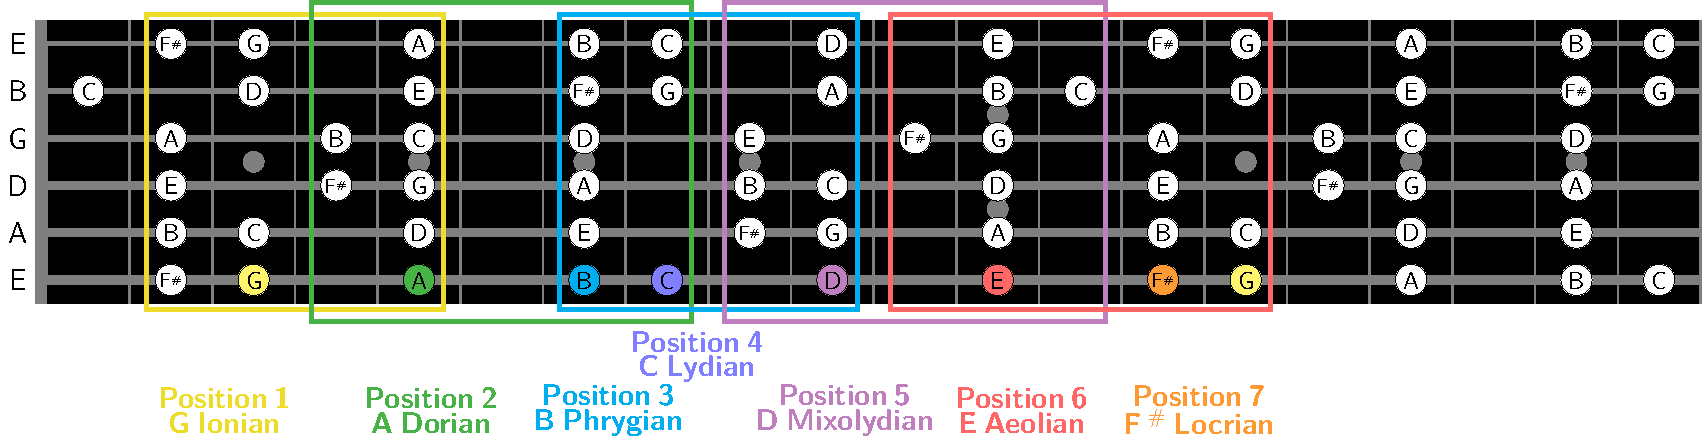
\includegraphics[scale=0.55, trim= {0cm 0cm 0cm 0cm}, clip]{gamme_majeure_manche/main.pdf}
	\scalebox{0.5}{%\documentclass{standalone}
%\usepackage{pgfplots} % Include package for TikZ and PGF plot
%\usepackage{anyfontsize} % enable to change the font size manually
%\usepackage{makecell}%
\usetikzlibrary{shapes.geometric}
\tikzset{
dot/.style = {circle, fill, minimum size=#1,
              inner sep=0pt, outer sep=0pt},
dot/.default = 6pt % size of the circle diameter 
}
 \renewcommand{\familydefault}{\sfdefault}

%\begin{document}
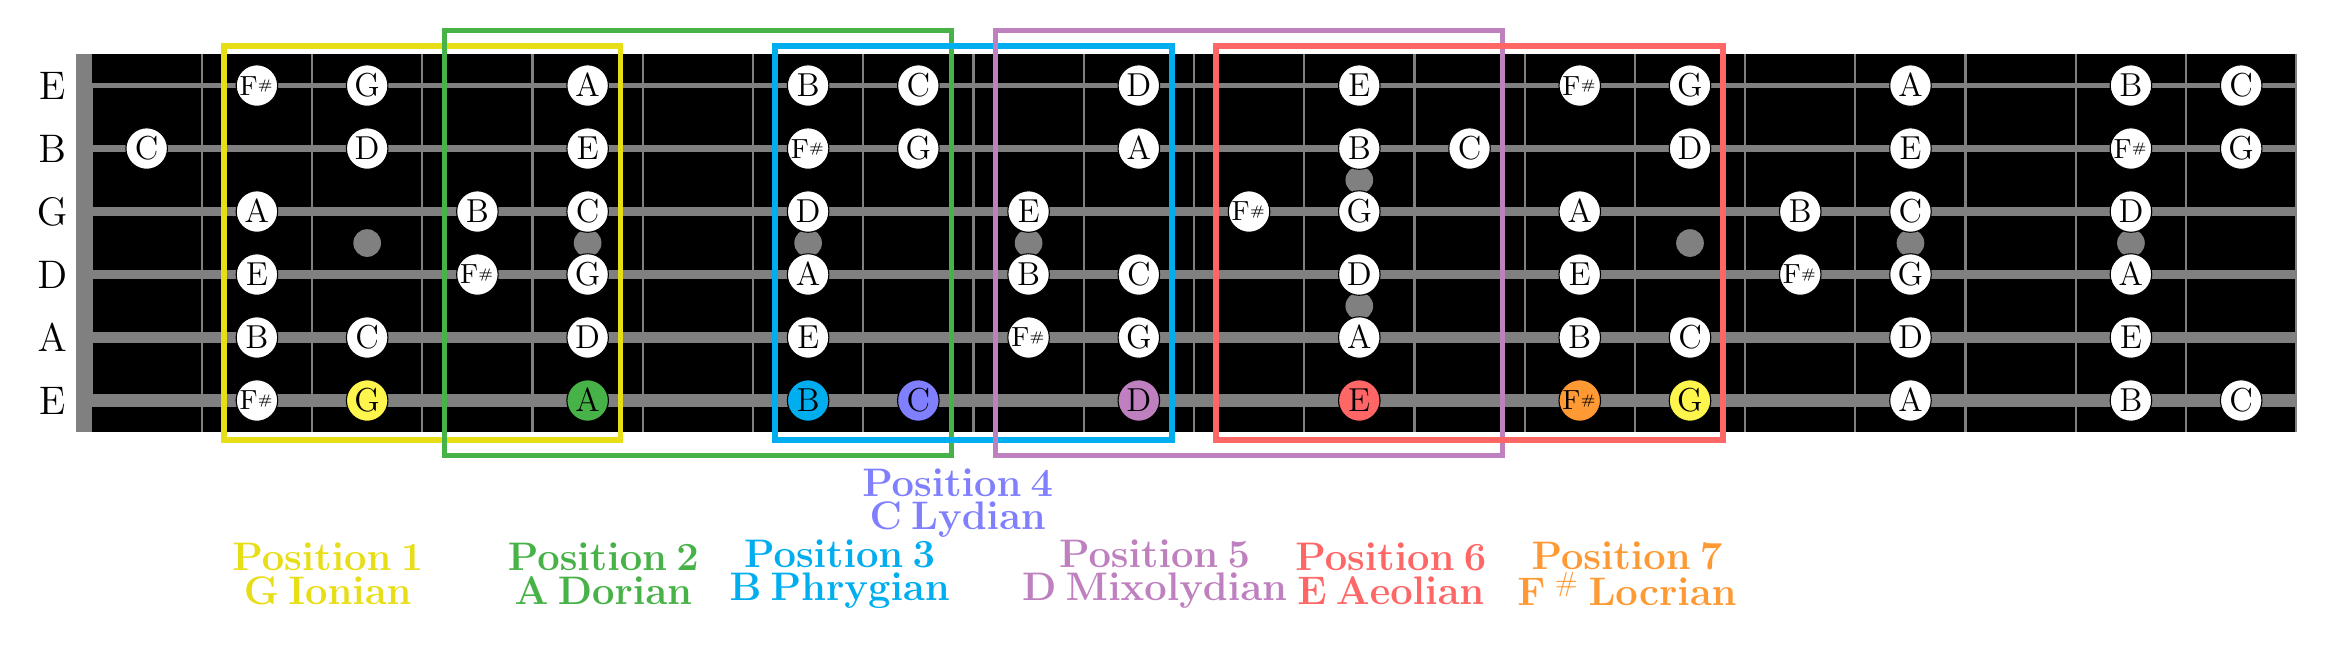
\begin{tikzpicture}[scale=1]
	\def \h{0.8}
	\def \fret{1.4} % 1.6
	\def \L{ 20*\fret }	
	\def \dot_size{5pt}
	\def \circ_size{15pt}
	
	\fill[black, line width=2] (0.0,-0.4) rectangle (20*\fret,4.4);
	\fill[black!50!white, line width=2] (-0.2,-0.4) rectangle (0,4.4);
	
	% Strings
	\draw[color=black!50!white, line width=2.0]  (-0.1, 5*\h) -- (\L,5*\h); % E
	\draw[color=black!50!white, line width=2.5]  (-0.1, 4*\h) -- (\L,4*\h); % B
	\draw[color=black!50!white, line width=3.0]  (-0.1, 3*\h) -- (\L,3*\h); % G
	\draw[color=black!50!white, line width=3.5]  (-0.1, 2*\h) -- (\L,2*\h); % D
	\draw[color=black!50!white, line width=4.0]  (-0.1, 1*\h) -- (\L,1*\h); % A
	\draw[color=black!50!white, line width=4.5]  (-0.1, 0*\h) -- (\L,0*\h); % E
	
	% Frets 0
	\draw[color=black!50!white, thick]  (-0.1, 0) -- (-0.1,5*\h); 
	\draw[color=black!50!white, thick]  (0, 0)   -- (0,5*\h); 
	
	% Fret 1-15
	\draw[color=black!50!white, thick]  (\fret,   -0.4)   -- (\fret,4.4);   
	\draw[color=black!50!white, thick]  (2*\fret, -0.4) -- (2*\fret,4.4); 
	\draw[color=black!50!white, thick]  (3*\fret, -0.4) -- (3*\fret,4.4); 
	\draw[color=black!50!white, thick]  (4*\fret, -0.4) -- (4*\fret,4.4); 
	\draw[color=black!50!white, thick]  (5*\fret, -0.4) -- (5*\fret,4.4); 
	\draw[color=black!50!white, thick]  (6*\fret, -0.4) -- (6*\fret,4.4); 
	\draw[color=black!50!white, thick]  (7*\fret, -0.4) -- (7*\fret,4.4); 
	\draw[color=black!50!white, thick]  (8*\fret, -0.4) -- (8*\fret,4.4); 
	\draw[color=black!50!white, thick]  (9*\fret, -0.4) -- (9*\fret,4.4); 
	\draw[color=black!50!white, thick]  (10*\fret, -0.4) -- (10*\fret,4.4); 
	\draw[color=black!50!white, thick]  (11*\fret, -0.4) -- (11*\fret,4.4); 
	\draw[color=black!50!white, thick]  (12*\fret, -0.4) -- (12*\fret,4.4); 
	\draw[color=black!50!white, thick]  (13*\fret, -0.4) -- (13*\fret,4.4); 
	\draw[color=black!50!white, thick]  (14*\fret, -0.4) -- (14*\fret,4.4); 
	\draw[color=black!50!white, thick]  (15*\fret, -0.4) -- (15*\fret,4.4); 
	\draw[color=black!50!white, thick]  (16*\fret, -0.4) -- (16*\fret,4.4); 
	\draw[color=black!50!white, thick]  (17*\fret, -0.4) -- (17*\fret,4.4); 
	\draw[color=black!50!white, thick]  (18*\fret, -0.4) -- (18*\fret,4.4); 
	\draw[color=black!50!white, thick]  (19*\fret, -0.4) -- (19*\fret,4.4); 
	\draw[color=black!50!white, thick]  (20*\fret, -0.4) -- (20*\fret,4.4); 
	
	% Dots
	\fill[black!50!white] (2.5*\fret,2.5*\h) circle (\dot_size); % fret 3
	\fill[black!50!white] (4.5*\fret,2.5*\h) circle (\dot_size); % fret 5
	\fill[black!50!white] (6.5*\fret,2.5*\h) circle (\dot_size); % fret 7
	\fill[black!50!white] (8.5*\fret,2.5*\h) circle (\dot_size); % fret 9
	\fill[black!50!white] (11.5*\fret,1.5*\h) circle (\dot_size); % fret 12
	\fill[black!50!white] (11.5*\fret,3.5*\h) circle (\dot_size); % fret 12
	\fill[black!50!white] (14.5*\fret,2.5*\h) circle (\dot_size); % fret 15
	\fill[black!50!white] (16.5*\fret,2.5*\h) circle (\dot_size); % fret 17
	\fill[black!50!white] (18.5*\fret,2.5*\h) circle (\dot_size); % fret 19
	
	% String names
	\draw[black] (-0.5,5*\h) node { {\Large E} };
	\draw[black] (-0.5,4*\h) node { {\Large B} };
	\draw[black] (-0.5,3*\h) node { {\Large G} };
	\draw[black] (-0.5,2*\h) node { {\Large D} };
	\draw[black] (-0.5,1*\h) node { {\Large A} };
	\draw[black] (-0.5,0*\h) node { {\Large E} };
	
	% Major scale (fret 1-5)
	\node[dot=\circ_size, fill=white,draw] at (1.5*\fret,0) { {\normalsize F}{\tiny $^\#$}};
	\node[dot=\circ_size, fill=yellow!70!white,draw] at (2.5*\fret,0) {{\large G}};
	\node[dot=\circ_size, fill=green!60!white!70!black, draw] at (4.5*\fret,0) {{\large A}};
	\node[dot=\circ_size, fill=white,draw] at (1.5*\fret,1*\h) {{\large B}};
	\node[dot=\circ_size, fill=white,draw] at (2.5*\fret,1*\h) {{\large C}};
	\node[dot=\circ_size, fill=white,draw] at (4.5*\fret,1*\h) {{\large D}};

	\node[dot=\circ_size, fill=white,draw] at (1.5*\fret,2*\h) {{\large E}};
	\node[dot=\circ_size, fill=white,draw] at (3.5*\fret,2*\h) {{\normalsize F}{\tiny $^\#$}};
	\node[dot=\circ_size, fill=white,draw] at (4.5*\fret,2*\h) {{\large G}};

	\node[dot=\circ_size, fill=white,draw] at (1.5*\fret,3*\h) {{\large A}};
	\node[dot=\circ_size, fill=white,draw] at (3.5*\fret,3*\h) {{\large B}};
	\node[dot=\circ_size, fill=white,draw] at (4.5*\fret,3*\h) {{\large C}};

	\node[dot=\circ_size, fill=white,draw] at (0.5*\fret,4*\h) {{\large C}};
	\node[dot=\circ_size, fill=white,draw] at (2.5*\fret,4*\h) {{\large D}};
	\node[dot=\circ_size, fill=white,draw] at (4.5*\fret,4*\h) {{\large E}};
	
	\node[dot=\circ_size, fill=white,draw] at (1.5*\fret,5*\h) {{\normalsize F}{\tiny $^\#$}};
	\node[dot=\circ_size, fill=white,draw] at (2.5*\fret,5*\h) {{\large G}};
	\node[dot=\circ_size, fill=white,draw] at (4.5*\fret,5*\h) {{\large A}};
	
	% Major scale (fret 7-10)
	\node[dot=\circ_size, fill=cyan,draw] at (6.5*\fret,0)    {{\large B}};
	\node[dot=\circ_size, fill=blue!50!white,draw] at (7.5*\fret,0)    {{\large C}};
	\node[dot=\circ_size, fill=blue!50!red!50!white,draw] at (9.5*\fret,0)    {{\large D}};
	
	\node[dot=\circ_size, fill=white,draw] at (6.5*\fret,1*\h) {{\large E}};
	\node[dot=\circ_size, fill=white,draw] at (8.5*\fret,1*\h) {{\large {\normalsize F}{\tiny $^\#$}}};
	\node[dot=\circ_size, fill=white,draw] at (9.5*\fret,1*\h) {{\large G}};
	
	\node[dot=\circ_size, fill=white,draw] at (6.5*\fret,2*\h) {{\large A}};
	\node[dot=\circ_size, fill=white,draw] at (8.5*\fret,2*\h) {{\large B}};
	\node[dot=\circ_size, fill=white,draw] at (9.5*\fret,2*\h) {{\large C}};
	
	\node[dot=\circ_size, fill=white,draw] at (6.5*\fret,3*\h) {{\large D}};
	\node[dot=\circ_size, fill=white,draw] at (8.5*\fret,3*\h) {{\large E}};
	
	\node[dot=\circ_size, fill=white,draw] at (6.5*\fret,4*\h) {{\large {\normalsize F}{\tiny $^\#$}}};
	\node[dot=\circ_size, fill=white,draw] at (7.5*\fret,4*\h) {{\large G}};
	\node[dot=\circ_size, fill=white,draw] at (9.5*\fret,4*\h) {{\large A}};
	
	\node[dot=\circ_size, fill=white,draw] at (6.5*\fret,5*\h) {{\large B}};
	\node[dot=\circ_size, fill=white,draw] at (7.5*\fret,5*\h) {{\large C}};
	\node[dot=\circ_size, fill=white,draw] at (9.5*\fret,5*\h) {{\large D}};
	
	% Major scale (fret 11-15)
	\node[dot=\circ_size, fill=red!60!white,   draw] at (11.5*\fret,0)    {{\large E}};
	\node[dot=\circ_size, fill=orange!80!white,draw] at (13.5*\fret,0)    {{\large {\normalsize F}{\tiny $^\#$}}};
	\node[dot=\circ_size, fill=yellow!70!white,draw] at (14.5*\fret,0)    {{\large G}};
	
	\node[dot=\circ_size, fill=white,draw] at (11.5*\fret,1*\h) {{\large A}};
	\node[dot=\circ_size, fill=white,draw] at (13.5*\fret,1*\h) {{\large B}};
	\node[dot=\circ_size, fill=white,draw] at (14.5*\fret,1*\h) {{\large C}};
	
	\node[dot=\circ_size, fill=white,draw] at (11.5*\fret,2*\h) {{\large D}};
	\node[dot=\circ_size, fill=white,draw] at (13.5*\fret,2*\h) {{\large E}};
	
	\node[dot=\circ_size, fill=white,draw] at (10.5*\fret,3*\h) {{\large {\normalsize F}{\tiny $^\#$}}};
	\node[dot=\circ_size, fill=white,draw] at (11.5*\fret,3*\h) {{\large G}};
	\node[dot=\circ_size, fill=white,draw] at (13.5*\fret,3*\h) {{\large A}};
	
	\node[dot=\circ_size, fill=white,draw] at (11.5*\fret,4*\h) {{\large B}};
	\node[dot=\circ_size, fill=white,draw] at (12.5*\fret,4*\h) {{\large C}};
	\node[dot=\circ_size, fill=white,draw] at (14.5*\fret,4*\h) {{\large D}};
	
	\node[dot=\circ_size, fill=white,draw] at (11.5*\fret,5*\h) {{\large E}};
	\node[dot=\circ_size, fill=white,draw] at (13.5*\fret,5*\h) {{\large {\normalsize F}{\tiny $^\#$}}};
	\node[dot=\circ_size, fill=white,draw] at (14.5*\fret,5*\h) {{\large G}};
	
	% Major scale (fret 16-20)
	\node[dot=\circ_size, fill=white,draw] at (16.5*\fret,0) {{\large A}};
	\node[dot=\circ_size, fill=white,draw] at (18.5*\fret,0) {{\large B}};
	\node[dot=\circ_size, fill=white,draw] at (19.5*\fret,0) {{\large C}};
	
	\node[dot=\circ_size, fill=white,draw] at (16.5*\fret,1*\h) {{\large D}};
	\node[dot=\circ_size, fill=white,draw] at (18.5*\fret,1*\h) {{\large E}};
	
	\node[dot=\circ_size, fill=white,draw] at (15.5*\fret,2*\h) {{\large {\normalsize F}{\tiny $^\#$}}};
	\node[dot=\circ_size, fill=white,draw] at (16.5*\fret,2*\h) {{\large G}};
	\node[dot=\circ_size, fill=white,draw] at (18.5*\fret,2*\h) {{\large A}};
	
	\node[dot=\circ_size, fill=white,draw] at (15.5*\fret,3*\h) {{\large B}};
	\node[dot=\circ_size, fill=white,draw] at (16.5*\fret,3*\h) {{\large C}};
	\node[dot=\circ_size, fill=white,draw] at (18.5*\fret,3*\h) {{\large D}};
	
	\node[dot=\circ_size, fill=white,draw] at (16.5*\fret,4*\h) {{\large E}};
	\node[dot=\circ_size, fill=white,draw] at (18.5*\fret,4*\h) {{\large {\normalsize F}{\tiny $^\#$}}};
	\node[dot=\circ_size, fill=white,draw] at (19.5*\fret,4*\h) {{\large G}};
	
	\node[dot=\circ_size, fill=white,draw] at (16.5*\fret,5*\h) {{\large A}};
	\node[dot=\circ_size, fill=white,draw] at (18.5*\fret,5*\h) {{\large B}};
	\node[dot=\circ_size, fill=white,draw] at (19.5*\fret,5*\h) {{\large C}};
	
	% Position 1 (ionien)
	\draw [draw=yellow!90!black,         line width=2] (1.2*\fret,-0.5) rectangle (4.8*\fret,4.5);
	% Position 2 (dorien)
	\draw [draw=green!60!white!70!black, line width=2] (3.2*\fret,-0.7) rectangle (7.8*\fret,4.7);
	% Position 3 (phrygien)
	\draw [draw=cyan,                    line width=2] (6.2*\fret,-0.5) rectangle (9.8*\fret,4.5);
	% Position 5 (mixolydien)
	\draw [draw=blue!50!red!50!white,    line width=2] (8.2*\fret,-0.7) rectangle (12.8*\fret,4.7);
	% Position 6 (eolien)
	\draw [draw=red!60!white,            line width=2] (10.2*\fret,-0.5) rectangle (14.8*\fret,4.5);
	
	% Mode names
	\draw[yellow!90!black,         anchor=center, text width=3.5cm, align=center] (3,-2.2) node { {\Large \textbf{Position~1 G~Ionian} }};
	\draw[green!60!white!70!black, anchor=center, text width=3.5cm, align=center] (6.5,-2.2) node { {\Large \textbf{Position~2 A~Dorian} }};
	\draw[cyan,                    anchor=center, text width=3.5cm, align=center] (9.5,-2.2) node { {\Large \textbf{Position~3 B~Phrygian} }};
	\draw[blue!50!white,           anchor=center, text width=3.5cm, align=center] (11,-1.3) node { {\Large \textbf{Position~4 C~Lydian} }};
	\draw[blue!50!red!50!white,    anchor=center, text width=3.5cm, align=center] (13.5,-2.2) node { {\Large \textbf{Position~5 D~Mixolydian} }};
	\draw[red!60!white,            anchor=center, text width=3.5cm, align=center] (16.5,-2.2) node { {\Large \textbf{Position~6 E~Aeolian} }};
	\draw[orange!80!white,         anchor=center, text width=3.5cm, align=center] (19.5,-2.2) node { {\Large \textbf{Position~7 F $^\#$~Locrian} }};
\end{tikzpicture}
%\end{document}}
	\caption{G Major scale on the fretboard}
	\label{fig:gamme_majeure_manche}
\end{figure}

\newpage
\subsection{Pentatonic scale}
% Figure
\begin{figure}[h!]
	\centering
	\hspace*{-2cm}
%	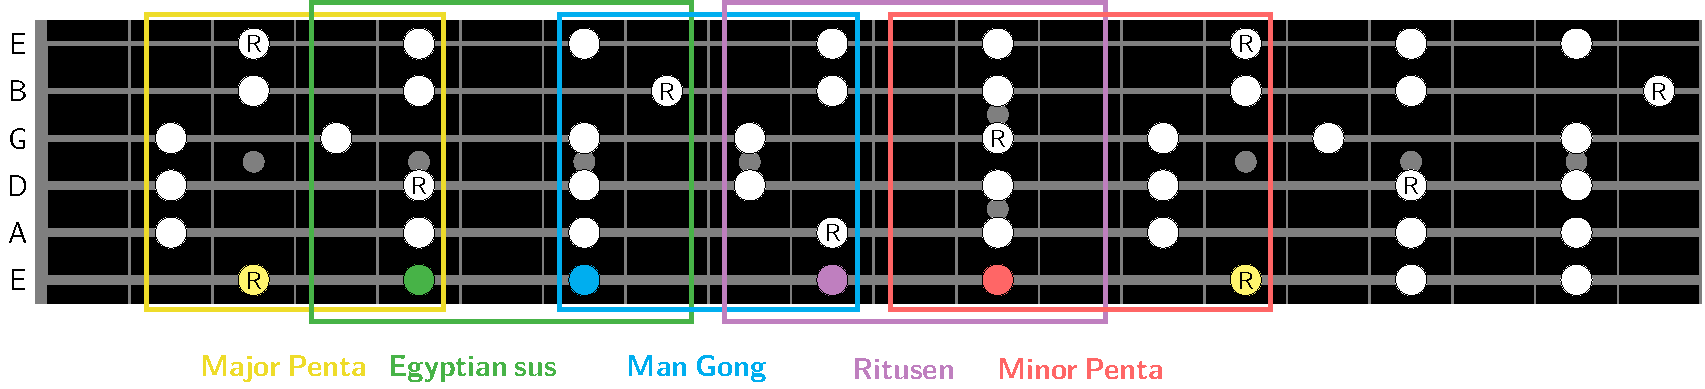
\includegraphics[scale=0.55, trim= {0cm 0cm 0cm 0cm}, clip]{gamme_penta_manche/main.pdf}
	\scalebox{0.5}{%\documentclass{standalone}
%\usepackage{pgfplots} % Include package for TikZ and PGF plot
%\usepackage{anyfontsize} % enable to change the font size manually
%\usepackage{makecell}%
\usetikzlibrary{shapes.geometric}
\tikzset{
dot/.style = {circle, fill, minimum size=#1,
              inner sep=0pt, outer sep=0pt},
dot/.default = 6pt % size of the circle diameter 
}
 \renewcommand{\familydefault}{\sfdefault}

%\begin{document}
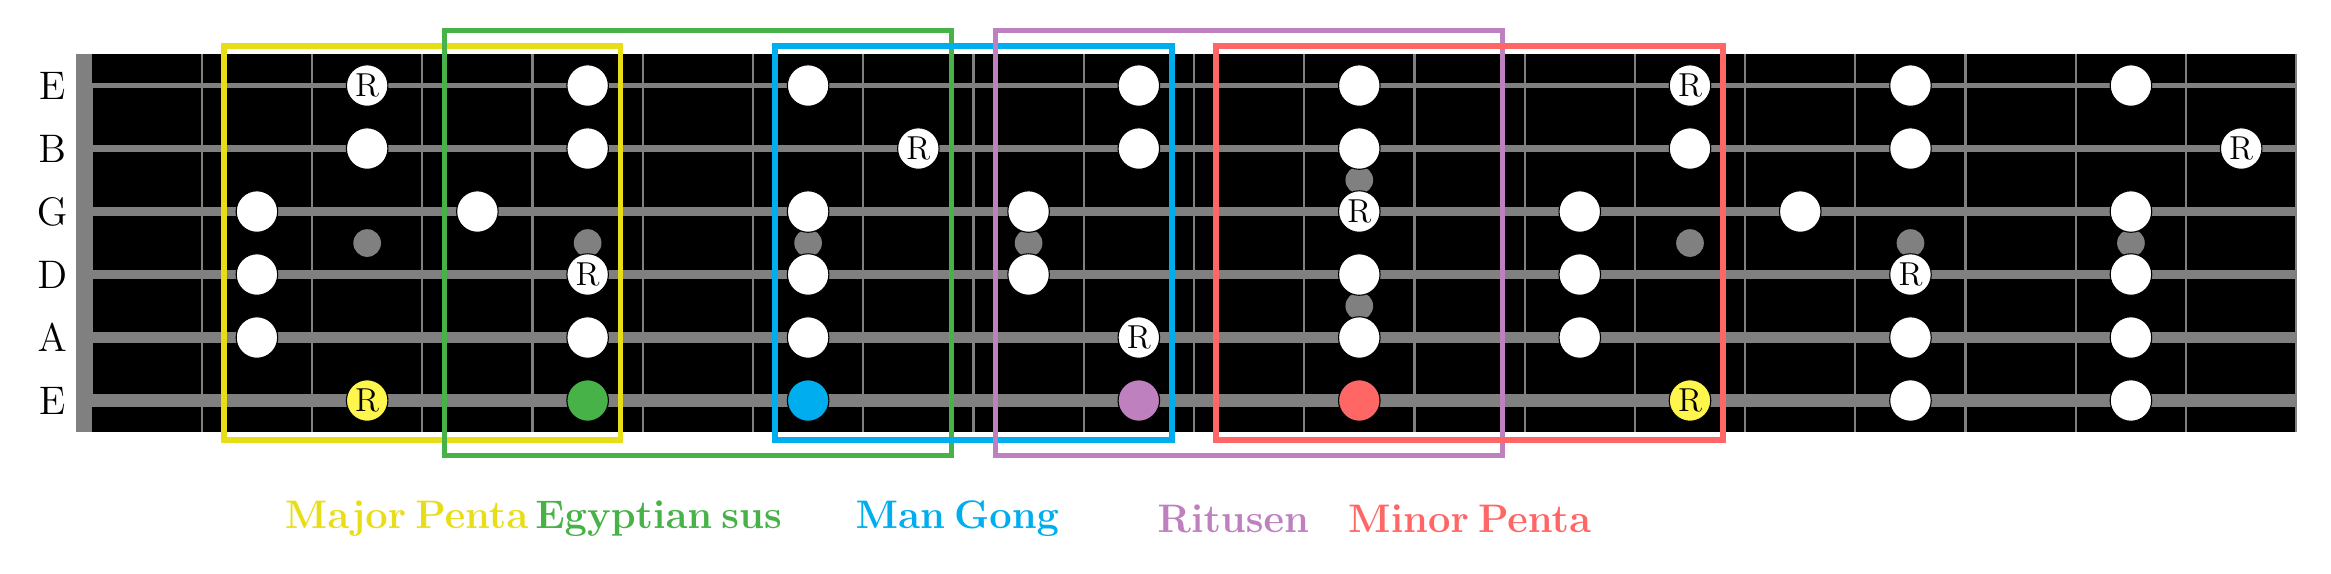
\begin{tikzpicture}[scale=1]
	\def \h{0.8}
	\def \fret{1.4} % 1.6
	\def \L{ 20*\fret }	
	\def \dot_size{5pt}
	\def \circ_size{15pt}
	
	\fill[black, line width=2] (0.0,-0.4) rectangle (20*\fret,4.4);
	\fill[black!50!white, line width=2] (-0.2,-0.4) rectangle (0,4.4);
	
	% Strings
	\draw[color=black!50!white, line width=2.0]  (-0.1, 5*\h) -- (\L,5*\h); % E
	\draw[color=black!50!white, line width=2.5]  (-0.1, 4*\h) -- (\L,4*\h); % B
	\draw[color=black!50!white, line width=3.0]  (-0.1, 3*\h) -- (\L,3*\h); % G
	\draw[color=black!50!white, line width=3.5]  (-0.1, 2*\h) -- (\L,2*\h); % D
	\draw[color=black!50!white, line width=4.0]  (-0.1, 1*\h) -- (\L,1*\h); % A
	\draw[color=black!50!white, line width=4.5]  (-0.1, 0*\h) -- (\L,0*\h); % E
	
	% Frets 0
	\draw[color=black!50!white, thick]  (-0.1, 0) -- (-0.1,5*\h); 
	\draw[color=black!50!white, thick]  (0, 0)   -- (0,5*\h); 
	
	% Fret 1-15
	\draw[color=black!50!white, thick]  (\fret,   -0.4)   -- (\fret,4.4);   
	\draw[color=black!50!white, thick]  (2*\fret, -0.4) -- (2*\fret,4.4); 
	\draw[color=black!50!white, thick]  (3*\fret, -0.4) -- (3*\fret,4.4); 
	\draw[color=black!50!white, thick]  (4*\fret, -0.4) -- (4*\fret,4.4); 
	\draw[color=black!50!white, thick]  (5*\fret, -0.4) -- (5*\fret,4.4); 
	\draw[color=black!50!white, thick]  (6*\fret, -0.4) -- (6*\fret,4.4); 
	\draw[color=black!50!white, thick]  (7*\fret, -0.4) -- (7*\fret,4.4); 
	\draw[color=black!50!white, thick]  (8*\fret, -0.4) -- (8*\fret,4.4); 
	\draw[color=black!50!white, thick]  (9*\fret, -0.4) -- (9*\fret,4.4); 
	\draw[color=black!50!white, thick]  (10*\fret, -0.4) -- (10*\fret,4.4); 
	\draw[color=black!50!white, thick]  (11*\fret, -0.4) -- (11*\fret,4.4); 
	\draw[color=black!50!white, thick]  (12*\fret, -0.4) -- (12*\fret,4.4); 
	\draw[color=black!50!white, thick]  (13*\fret, -0.4) -- (13*\fret,4.4); 
	\draw[color=black!50!white, thick]  (14*\fret, -0.4) -- (14*\fret,4.4); 
	\draw[color=black!50!white, thick]  (15*\fret, -0.4) -- (15*\fret,4.4); 
	\draw[color=black!50!white, thick]  (16*\fret, -0.4) -- (16*\fret,4.4); 
	\draw[color=black!50!white, thick]  (17*\fret, -0.4) -- (17*\fret,4.4); 
	\draw[color=black!50!white, thick]  (18*\fret, -0.4) -- (18*\fret,4.4); 
	\draw[color=black!50!white, thick]  (19*\fret, -0.4) -- (19*\fret,4.4); 
	\draw[color=black!50!white, thick]  (20*\fret, -0.4) -- (20*\fret,4.4); 
	
	% Dots
	\fill[black!50!white] (2.5*\fret,2.5*\h) circle (\dot_size); % fret 3
	\fill[black!50!white] (4.5*\fret,2.5*\h) circle (\dot_size); % fret 5
	\fill[black!50!white] (6.5*\fret,2.5*\h) circle (\dot_size); % fret 7
	\fill[black!50!white] (8.5*\fret,2.5*\h) circle (\dot_size); % fret 9
	\fill[black!50!white] (11.5*\fret,1.5*\h) circle (\dot_size); % fret 12
	\fill[black!50!white] (11.5*\fret,3.5*\h) circle (\dot_size); % fret 12
	\fill[black!50!white] (14.5*\fret,2.5*\h) circle (\dot_size); % fret 15
	\fill[black!50!white] (16.5*\fret,2.5*\h) circle (\dot_size); % fret 17
	\fill[black!50!white] (18.5*\fret,2.5*\h) circle (\dot_size); % fret 19
	
	% String names
	\draw[black] (-0.5,5*\h) node { {\Large E} };
	\draw[black] (-0.5,4*\h) node { {\Large B} };
	\draw[black] (-0.5,3*\h) node { {\Large G} };
	\draw[black] (-0.5,2*\h) node { {\Large D} };
	\draw[black] (-0.5,1*\h) node { {\Large A} };
	\draw[black] (-0.5,0*\h) node { {\Large E} };
	
	% Major scale (fret 1-5)
	%\node[dot=\circ_size, fill=white,draw] at (1.5*\fret,0) { {\normalsize F}{\tiny $^\#$}};
	\node[dot=\circ_size, fill=yellow!70!white,draw] at (2.5*\fret,0) {{\large R}};
	\node[dot=\circ_size, fill=green!60!white!70!black, draw] at (4.5*\fret,0) {{\large }};
	\node[dot=\circ_size, fill=white,draw] at (1.5*\fret,1*\h) {{\large }};
	%\node[dot=\circ_size, fill=white,draw] at (2.5*\fret,1*\h) {{\large C}};
	\node[dot=\circ_size, fill=white,draw] at (4.5*\fret,1*\h) {{\large }};

	\node[dot=\circ_size, fill=white,draw] at (1.5*\fret,2*\h) {{\large }};
	%\node[dot=\circ_size, fill=white,draw] at (3.5*\fret,2*\h) {{\normalsize F}{\tiny $^\#$}};
	\node[dot=\circ_size, fill=white,draw] at (4.5*\fret,2*\h) {{\large R}};

	\node[dot=\circ_size, fill=white,draw] at (1.5*\fret,3*\h) {{\large }};
	\node[dot=\circ_size, fill=white,draw] at (3.5*\fret,3*\h) {{\large }};
	%\node[dot=\circ_size, fill=white,draw] at (4.5*\fret,3*\h) {{\large C}};

	%\node[dot=\circ_size, fill=white,draw] at (0.5*\fret,4*\h) {{\large C}};
	\node[dot=\circ_size, fill=white,draw] at (2.5*\fret,4*\h) {{\large }};
	\node[dot=\circ_size, fill=white,draw] at (4.5*\fret,4*\h) {{\large }};
	
	%\node[dot=\circ_size, fill=white,draw] at (1.5*\fret,5*\h) {{\normalsize F}{\tiny $^\#$}};
	\node[dot=\circ_size, fill=white,draw] at (2.5*\fret,5*\h) {{\large R}};
	\node[dot=\circ_size, fill=white,draw] at (4.5*\fret,5*\h) {{\large }};
	
	% Major scale (fret 7-10)
	\node[dot=\circ_size, fill=cyan,draw] at (6.5*\fret,0)    {{\large }};
	%\node[dot=\circ_size, fill=blue!50!white,draw] at (7.5*\fret,0)    {{\large C}};
	\node[dot=\circ_size, fill=blue!50!red!50!white,draw] at (9.5*\fret,0)    {{\large }};
	
	\node[dot=\circ_size, fill=white,draw] at (6.5*\fret,1*\h) {{\large }};
	%\node[dot=\circ_size, fill=white,draw] at (8.5*\fret,1*\h) {{\large {\normalsize F}{\tiny $^\#$}}};
	\node[dot=\circ_size, fill=white,draw] at (9.5*\fret,1*\h) {{\large R}};
	
	\node[dot=\circ_size, fill=white,draw] at (6.5*\fret,2*\h) {{\large }};
	\node[dot=\circ_size, fill=white,draw] at (8.5*\fret,2*\h) {{\large }};
	%\node[dot=\circ_size, fill=white,draw] at (9.5*\fret,2*\h) {{\large C}};
	
	\node[dot=\circ_size, fill=white,draw] at (6.5*\fret,3*\h) {{\large }};
	\node[dot=\circ_size, fill=white,draw] at (8.5*\fret,3*\h) {{\large }};
	
	%\node[dot=\circ_size, fill=white,draw] at (6.5*\fret,4*\h) {{\large {\normalsize F}{\tiny $^\#$}}};
	\node[dot=\circ_size, fill=white,draw] at (7.5*\fret,4*\h) {{\large R}};
	\node[dot=\circ_size, fill=white,draw] at (9.5*\fret,4*\h) {{\large }};
	
	\node[dot=\circ_size, fill=white,draw] at (6.5*\fret,5*\h) {{\large }};
	%\node[dot=\circ_size, fill=white,draw] at (7.5*\fret,5*\h) {{\large C}};
	\node[dot=\circ_size, fill=white,draw] at (9.5*\fret,5*\h) {{\large }};
	
	% Major scale (fret 11-15)
	\node[dot=\circ_size, fill=red!60!white,   draw] at (11.5*\fret,0)    {{\large }};
	%\node[dot=\circ_size, fill=orange!80!white,draw] at (13.5*\fret,0)    {{\large {\normalsize F}{\tiny $^\#$}}};
	\node[dot=\circ_size, fill=yellow!70!white,draw] at (14.5*\fret,0)    {{\large R}};
	
	\node[dot=\circ_size, fill=white,draw] at (11.5*\fret,1*\h) {{\large }};
	\node[dot=\circ_size, fill=white,draw] at (13.5*\fret,1*\h) {{\large }};
	%\node[dot=\circ_size, fill=white,draw] at (14.5*\fret,1*\h) {{\large C}};
	
	\node[dot=\circ_size, fill=white,draw] at (11.5*\fret,2*\h) {{\large }};
	\node[dot=\circ_size, fill=white,draw] at (13.5*\fret,2*\h) {{\large }};
	
	%\node[dot=\circ_size, fill=white,draw] at (10.5*\fret,3*\h) {{\large {\normalsize F}{\tiny $^\#$}}};
	\node[dot=\circ_size, fill=white,draw] at (11.5*\fret,3*\h) {{\large R}};
	\node[dot=\circ_size, fill=white,draw] at (13.5*\fret,3*\h) {{\large }};
	
	\node[dot=\circ_size, fill=white,draw] at (11.5*\fret,4*\h) {{\large }};
	%\node[dot=\circ_size, fill=white,draw] at (12.5*\fret,4*\h) {{\large C}};
	\node[dot=\circ_size, fill=white,draw] at (14.5*\fret,4*\h) {{\large }};
	
	\node[dot=\circ_size, fill=white,draw] at (11.5*\fret,5*\h) {{\large }};
	%\node[dot=\circ_size, fill=white,draw] at (13.5*\fret,5*\h) {{\large {\normalsize F}{\tiny $^\#$}}};
	\node[dot=\circ_size, fill=white,draw] at (14.5*\fret,5*\h) {{\large R}};
	
	% Major scale (fret 16-20)
	\node[dot=\circ_size, fill=white,draw] at (16.5*\fret,0) {{\large }};
	\node[dot=\circ_size, fill=white,draw] at (18.5*\fret,0) {{\large }};
	%\node[dot=\circ_size, fill=white,draw] at (19.5*\fret,0) {{\large C}};
	
	\node[dot=\circ_size, fill=white,draw] at (16.5*\fret,1*\h) {{\large }};
	\node[dot=\circ_size, fill=white,draw] at (18.5*\fret,1*\h) {{\large }};
	
	%\node[dot=\circ_size, fill=white,draw] at (15.5*\fret,2*\h) {{\large {\normalsize F}{\tiny $^\#$}}};
	\node[dot=\circ_size, fill=white,draw] at (16.5*\fret,2*\h) {{\large R}};
	\node[dot=\circ_size, fill=white,draw] at (18.5*\fret,2*\h) {{\large }};
	
	\node[dot=\circ_size, fill=white,draw] at (15.5*\fret,3*\h) {{\large }};
	%\node[dot=\circ_size, fill=white,draw] at (16.5*\fret,3*\h) {{\large C}};
	\node[dot=\circ_size, fill=white,draw] at (18.5*\fret,3*\h) {{\large }};
	
	\node[dot=\circ_size, fill=white,draw] at (16.5*\fret,4*\h) {{\large }};
	%\node[dot=\circ_size, fill=white,draw] at (18.5*\fret,4*\h) {{\large {\normalsize F}{\tiny $^\#$}}};
	\node[dot=\circ_size, fill=white,draw] at (19.5*\fret,4*\h) {{\large R}};
	
	\node[dot=\circ_size, fill=white,draw] at (16.5*\fret,5*\h) {{\large }};
	\node[dot=\circ_size, fill=white,draw] at (18.5*\fret,5*\h) {{\large }};
	%\node[dot=\circ_size, fill=white,draw] at (19.5*\fret,5*\h) {{\large C}};
	
	% Position 1 (ionien)
	\draw [draw=yellow!90!black,         line width=2] (1.2*\fret,-0.5) rectangle (4.8*\fret,4.5);
	% Position 2 (dorien)
	\draw [draw=green!60!white!70!black, line width=2] (3.2*\fret,-0.7) rectangle (7.8*\fret,4.7);
	% Position 3 (phrygien)
	\draw [draw=cyan,                    line width=2] (6.2*\fret,-0.5) rectangle (9.8*\fret,4.5);
	% Position 5 (mixolydien)
	\draw [draw=blue!50!red!50!white,    line width=2] (8.2*\fret,-0.7) rectangle (12.8*\fret,4.7);
	% Position 6 (eolien)
	\draw [draw=red!60!white,            line width=2] (10.2*\fret,-0.5) rectangle (14.8*\fret,4.5);
	
	% Mode names
	\draw[yellow!90!black,         anchor=center, text width=3.5cm, align=center] (4,  -1.5) node { {\Large \textbf{Major Penta} }};
	\draw[green!60!white!70!black, anchor=center, text width=3.5cm, align=center] (7.2,-1.5) node { {\Large \textbf{Egyptian sus} }};
	\draw[cyan,                    anchor=center, text width=3.5cm, align=center] (11,-1.5) node { {\Large \textbf{Man Gong}}};
	%\draw[blue!50!white,           anchor=center, text width=3.5cm, align=center] (12.2,-1.3) node { {\Large \textbf{Position~4} }};
	\draw[blue!50!red!50!white,    anchor=center, text width=3.5cm, align=center] (14.5,-1.5) node { {\Large \textbf{Ritusen} }};
	\draw[red!60!white,            anchor=center, text width=3.5cm, align=center] (17.5,-1.5) node { {\Large \textbf{Minor Penta} }};
	%\draw[orange!80!white,         anchor=center, text width=3.5cm, align=center] (21.8,-2.2) node { {\Large \textbf{Position~7} }};
\end{tikzpicture}
%\end{document}}
	\caption{Pattern of pentatonic scales}
	\label{fig:gammme_penta_manche}
\end{figure}

\newpage
\subsection{Blues}


% Table
\begin{table*}[!h]
	\caption{Blues scales (relative to the major scale)}
	\centering
	%\begin{adjustwidth}{0cm}{}
	\begin{tabular}{l|cccccccc}
		Scale name  & \multicolumn{8}{c}{Formula} \\
		\hline \hline \vspace{-0.4cm} \\
		Blues Major   & 1 & 2  & \textcolor{red}{b3} & 3  &   -   & 5  & 6  &  -  \\
		Blues minor   & 1 &  - & b3 & 4  & \textcolor{red}{b5} &  5  & - &  b7 \\
	\end{tabular}
	\label{tab: }
	%\end{adjustwidth}
\end{table*}

% Table
% % Jake Lizzio
\begin{table*}[!h]
	\caption{Basic 12 bar major blues}
	\centering
	\begin{tabular}{| c | c | c | c |}
		\hline
		\phantom{x}I7\phantom{x} & \phantom{x}I7\phantom{x} & \phantom{x}I7\phantom{x} & \phantom{x}I7\phantom{x}  \\
		\hline
		\phantom{x}IV7\phantom{x} & \phantom{x}IV7\phantom{x} & \phantom{x}I7\phantom{x} & \phantom{x}I7\phantom{x}  \\
		\hline
		\phantom{x}V7\phantom{x} & \phantom{x}IV7\phantom{x} & \phantom{x}I7\phantom{x} & \phantom{x}I7\phantom{x}  \\
		\hline
	\end{tabular}
	\label{tab: }
\end{table*}

\begin{table*}[!h]
	\caption{Basic 12 bar minor blues}
	\centering
	\begin{tabular}{| c | c | c | c |}
		\hline
		\phantom{x}i7\phantom{x} & \phantom{x}i7\phantom{x} & \phantom{x}i7\phantom{x} & \phantom{x}i7\phantom{x}  \\
		\hline
		\phantom{x}iv7\phantom{x} & \phantom{x}iv7\phantom{x} & \phantom{x}i7\phantom{x} & \phantom{x}i7\phantom{x}  \\
		\hline
		\phantom{x}v7 or V7\phantom{x} & \phantom{x}iv7\phantom{x} & \phantom{x}i7\phantom{x} & \phantom{x}V7\phantom{x}  \\
		\hline
	\end{tabular}
	\label{tab: }
\end{table*}

\begin{table*}[!h]
	\caption{Basic 12 bar major blues with a \textit{quick change} and \textit{turnaroun}d}
	\centering
	\begin{tabular}{| c | c | c | c |}
		\hline
		\phantom{x}I7\phantom{x} & \phantom{x}\textbf{IV7}\phantom{x} & \phantom{x}I7\phantom{x} & \phantom{x}I7\phantom{x}  \\
		\hline
		\phantom{x}IV7\phantom{x} & \phantom{x}IV7\phantom{x} & \phantom{x}I7\phantom{x} & \phantom{x}I7\phantom{x}  \\
		\hline
		\phantom{x}V7\phantom{x} & \phantom{x}IV7\phantom{x} & \phantom{x}I7 - \textbf{vi7} & \textbf{ii7} - V7\phantom{x}  \\
		\hline
	\end{tabular}
	\label{tab: }
\end{table*}

% Figure
\begin{figure}[h!]
	\centering
	\hspace*{-1cm}
	\scalebox{0.7}{
\renewcommand{\familydefault}{\sfdefault}

%\begin{document}
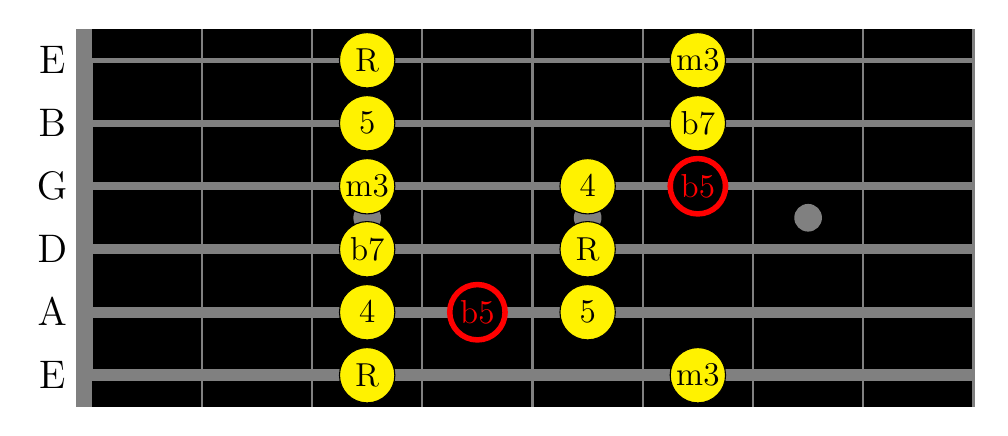
\begin{tikzpicture}[scale=1]
	\def \h{0.8}
	\def \fret{1.4} % 1.6
	\def \L{ 8*\fret }	
	\def \dot_size{5pt}
	\def \circ_size{15pt}
	
	\fill[black, line width=2] (0.0,-0.4) rectangle (8*\fret,4.4);
	\fill[black!50!white, line width=2] (-0.2,-0.4) rectangle (0,4.4);
	
	% Strings
	\draw[color=black!50!white, line width=2.0]  (-0.1, 5*\h) -- (\L,5*\h); % E
	\draw[color=black!50!white, line width=2.5]  (-0.1, 4*\h) -- (\L,4*\h); % B
	\draw[color=black!50!white, line width=3.0]  (-0.1, 3*\h) -- (\L,3*\h); % G
	\draw[color=black!50!white, line width=3.5]  (-0.1, 2*\h) -- (\L,2*\h); % D
	\draw[color=black!50!white, line width=4.0]  (-0.1, 1*\h) -- (\L,1*\h); % A
	\draw[color=black!50!white, line width=4.5]  (-0.1, 0*\h) -- (\L,0*\h); % E
	
	% Frets 0
	\draw[color=black!50!white, thick]  (-0.1, 0) -- (-0.1,5*\h); 
	\draw[color=black!50!white, thick]  (0, 0)   -- (0,5*\h); 
	
	% Fret 1-15
	\draw[color=black!50!white, thick]  (\fret,   -0.4)   -- (\fret,4.4);   
	\draw[color=black!50!white, thick]  (2*\fret, -0.4) -- (2*\fret,4.4); 
	\draw[color=black!50!white, thick]  (3*\fret, -0.4) -- (3*\fret,4.4); 
	\draw[color=black!50!white, thick]  (4*\fret, -0.4) -- (4*\fret,4.4); 
	\draw[color=black!50!white, thick]  (5*\fret, -0.4) -- (5*\fret,4.4); 
	\draw[color=black!50!white, thick]  (6*\fret, -0.4) -- (6*\fret,4.4); 
	\draw[color=black!50!white, thick]  (7*\fret, -0.4) -- (7*\fret,4.4); 
	\draw[color=black!50!white, thick]  (8*\fret, -0.4) -- (8*\fret,4.4); 
%	\draw[color=black!50!white, thick]  (9*\fret, -0.4) -- (9*\fret,4.4); 
%	\draw[color=black!50!white, thick]  (10*\fret, -0.4) -- (10*\fret,4.4); 
%	\draw[color=black!50!white, thick]  (11*\fret, -0.4) -- (11*\fret,4.4); 
%	\draw[color=black!50!white, thick]  (12*\fret, -0.4) -- (12*\fret,4.4); 
%	\draw[color=black!50!white, thick]  (13*\fret, -0.4) -- (13*\fret,4.4); 
%	\draw[color=black!50!white, thick]  (14*\fret, -0.4) -- (14*\fret,4.4); 
%	\draw[color=black!50!white, thick]  (15*\fret, -0.4) -- (15*\fret,4.4); 
%	\draw[color=black!50!white, thick]  (16*\fret, -0.4) -- (16*\fret,4.4); 
%	\draw[color=black!50!white, thick]  (17*\fret, -0.4) -- (17*\fret,4.4); 
%	\draw[color=black!50!white, thick]  (18*\fret, -0.4) -- (18*\fret,4.4); 
%	\draw[color=black!50!white, thick]  (19*\fret, -0.4) -- (19*\fret,4.4); 
%	\draw[color=black!50!white, thick]  (20*\fret, -0.4) -- (20*\fret,4.4); 
	
	% Dots
	\fill[black!50!white] (2.5*\fret,2.5*\h) circle (\dot_size); % fret 3
	\fill[black!50!white] (4.5*\fret,2.5*\h) circle (\dot_size); % fret 5
	\fill[black!50!white] (6.5*\fret,2.5*\h) circle (\dot_size); % fret 7
%	\fill[black!50!white] (8.5*\fret,2.5*\h) circle (\dot_size); % fret 9
%	\fill[black!50!white] (11.5*\fret,1.5*\h) circle (\dot_size); % fret 12
%	\fill[black!50!white] (11.5*\fret,3.5*\h) circle (\dot_size); % fret 12
%	\fill[black!50!white] (14.5*\fret,2.5*\h) circle (\dot_size); % fret 15
%	\fill[black!50!white] (16.5*\fret,2.5*\h) circle (\dot_size); % fret 17
%	\fill[black!50!white] (18.5*\fret,2.5*\h) circle (\dot_size); % fret 19
	
	% String names
	\draw[black] (-0.5,5*\h) node { {\Large E} };
	\draw[black] (-0.5,4*\h) node { {\Large B} };
	\draw[black] (-0.5,3*\h) node { {\Large G} };
	\draw[black] (-0.5,2*\h) node { {\Large D} };
	\draw[black] (-0.5,1*\h) node { {\Large A} };
	\draw[black] (-0.5,0*\h) node { {\Large E} };
	
	% Major scale (fret 1-5)
	%\node[dot=\circ_size, fill=white,draw] at (1.5*\fret,0) { {\normalsize F}{\tiny $^\#$}};
%	\node[dot=\circ_size, fill=yellow,draw] at (2.5*\fret,0) {{\large \textcolor{red}{R}}};    % Root
%	\node[dot=\circ_size, fill=yellow, draw] at (4.5*\fret,0) {{\large 2}};
%	\node[dot=\circ_size, fill=yellow,draw] at (5.5*\fret,0*\h) {{\large \textcolor{red}{m3}}};
%	\node[dot=\circ_size, fill=yellow,draw] at (1.5*\fret,1*\h) {{\large M3}};
%	\node[dot=\circ_size, fill=yellow,draw] at (4.5*\fret,1*\h) {{\large 5}};
%	\node[dot=\circ_size, fill=yellow,draw] at (1.5*\fret,2*\h) {{\large 6}};
%	\node[dot=\circ_size, fill=yellow,draw] at (4.5*\fret,2*\h) {{\large R}}; % Root
%	\node[dot=\circ_size, fill=yellow,draw] at (1.5*\fret,3*\h) {{\large 2}};
%	\node[dot=\circ_size, fill=yellow,draw] at (2.5*\fret,3*\h) {{\large m3}};
%	\node[dot=\circ_size, fill=yellow,draw] at (3.5*\fret,3*\h) {{\large M3}};
%	\node[dot=\circ_size, fill=yellow,draw] at (2.5*\fret,4*\h) {{\large 5}};
%	\node[dot=\circ_size, fill=yellow,draw] at (4.5*\fret,4*\h) {{\large 6}};
%	\node[dot=\circ_size, fill=yellow,draw] at (2.5*\fret,5*\h) {{\large R}};
%	\node[dot=\circ_size, fill=yellow,draw] at (4.5*\fret,5*\h) {{\large 2}};
%	\node[dot=\circ_size, fill=yellow,draw] at (5.5*\fret,5*\h) {{m3}};
	
	\node[dot=20pt, fill=yellow,draw] at (2.5*\fret,0) {{\large \textcolor{black}{R}}};    % Root
	\node[dot=20pt, fill=yellow,draw] at (5.5*\fret,0) {{\large \textcolor{black}{m3}}};    % m3
	\node[dot=20pt, fill=yellow,draw] at (2.5*\fret,1*\h) {{\large \textcolor{black}{4}}};    % 4
	\node[dot=20pt, draw=red, line width=2,draw] at (3.5*\fret,1*\h) {{\large \textcolor{red}{b5}}};
	\node[dot=20pt, fill=yellow,draw] at (4.5*\fret,1*\h) {{\large \textcolor{black}{5}}};
	\node[dot=20pt, fill=yellow,draw] at (2.5*\fret,2*\h) {{\large \textcolor{black}{b7}}};
	\node[dot=20pt, fill=yellow,draw] at (4.5*\fret,2*\h) {{\large \textcolor{black}{R}}};
	\node[dot=20pt, fill=yellow,draw] at (2.5*\fret,3*\h) {{\large \textcolor{black}{m3}}};
	\node[dot=20pt, fill=yellow,draw] at (4.5*\fret,3*\h) {{\large \textcolor{black}{4}}};
	\node[dot=20pt, draw=red, line width=2,draw] at (5.5*\fret,3*\h) {{\large \textcolor{red}{b5}}};
	\node[dot=20pt, fill=yellow,draw] at (2.5*\fret,4*\h) {{\large \textcolor{black}{5}}};
	\node[dot=20pt, fill=yellow,draw] at (5.5*\fret,4*\h) {{\large \textcolor{black}{b7}}};
	\node[dot=20pt, fill=yellow,draw] at (2.5*\fret,5*\h) {{\large \textcolor{black}{R}}};
	\node[dot=20pt, fill=yellow,draw] at (5.5*\fret,5*\h) {{\large \textcolor{black}{m3}}};
	
\end{tikzpicture}
%\end{document}









}
%	\vspace{10cm}
	\hspace*{-1cm}
	\scalebox{0.7}{
\renewcommand{\familydefault}{\sfdefault}

%\begin{document}
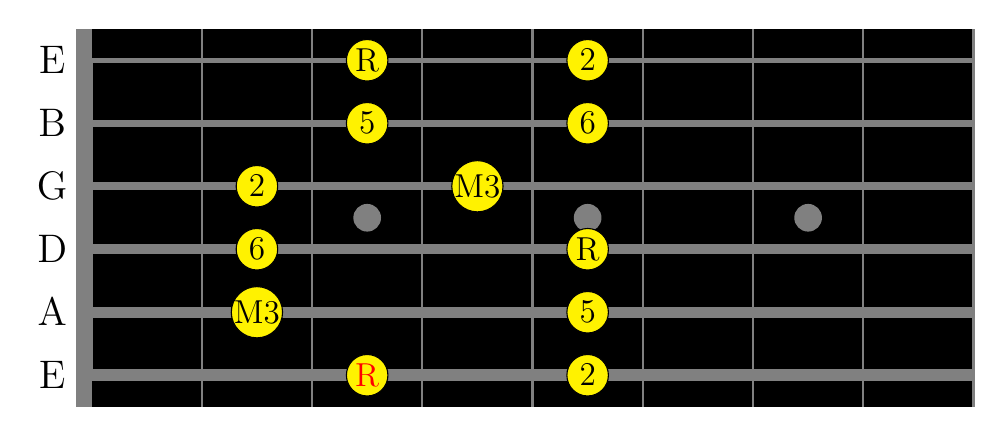
\begin{tikzpicture}[scale=1]
	\def \h{0.8}
	\def \fret{1.4} % 1.6
	\def \L{ 8*\fret }	
	\def \dot_size{5pt}
	\def \circ_size{15pt}
	
	\fill[black, line width=2] (0.0,-0.4) rectangle (8*\fret,4.4);
	\fill[black!50!white, line width=2] (-0.2,-0.4) rectangle (0,4.4);
	
	% Strings
	\draw[color=black!50!white, line width=2.0]  (-0.1, 5*\h) -- (\L,5*\h); % E
	\draw[color=black!50!white, line width=2.5]  (-0.1, 4*\h) -- (\L,4*\h); % B
	\draw[color=black!50!white, line width=3.0]  (-0.1, 3*\h) -- (\L,3*\h); % G
	\draw[color=black!50!white, line width=3.5]  (-0.1, 2*\h) -- (\L,2*\h); % D
	\draw[color=black!50!white, line width=4.0]  (-0.1, 1*\h) -- (\L,1*\h); % A
	\draw[color=black!50!white, line width=4.5]  (-0.1, 0*\h) -- (\L,0*\h); % E
	
	% Frets 0
	\draw[color=black!50!white, thick]  (-0.1, 0) -- (-0.1,5*\h); 
	\draw[color=black!50!white, thick]  (0, 0)   -- (0,5*\h); 
	
	% Fret 1-15
	\draw[color=black!50!white, thick]  (\fret,   -0.4)   -- (\fret,4.4);   
	\draw[color=black!50!white, thick]  (2*\fret, -0.4) -- (2*\fret,4.4); 
	\draw[color=black!50!white, thick]  (3*\fret, -0.4) -- (3*\fret,4.4); 
	\draw[color=black!50!white, thick]  (4*\fret, -0.4) -- (4*\fret,4.4); 
	\draw[color=black!50!white, thick]  (5*\fret, -0.4) -- (5*\fret,4.4); 
	\draw[color=black!50!white, thick]  (6*\fret, -0.4) -- (6*\fret,4.4); 
	\draw[color=black!50!white, thick]  (7*\fret, -0.4) -- (7*\fret,4.4); 
	\draw[color=black!50!white, thick]  (8*\fret, -0.4) -- (8*\fret,4.4); 
%	\draw[color=black!50!white, thick]  (9*\fret, -0.4) -- (9*\fret,4.4); 
%	\draw[color=black!50!white, thick]  (10*\fret, -0.4) -- (10*\fret,4.4); 
%	\draw[color=black!50!white, thick]  (11*\fret, -0.4) -- (11*\fret,4.4); 
%	\draw[color=black!50!white, thick]  (12*\fret, -0.4) -- (12*\fret,4.4); 
%	\draw[color=black!50!white, thick]  (13*\fret, -0.4) -- (13*\fret,4.4); 
%	\draw[color=black!50!white, thick]  (14*\fret, -0.4) -- (14*\fret,4.4); 
%	\draw[color=black!50!white, thick]  (15*\fret, -0.4) -- (15*\fret,4.4); 
%	\draw[color=black!50!white, thick]  (16*\fret, -0.4) -- (16*\fret,4.4); 
%	\draw[color=black!50!white, thick]  (17*\fret, -0.4) -- (17*\fret,4.4); 
%	\draw[color=black!50!white, thick]  (18*\fret, -0.4) -- (18*\fret,4.4); 
%	\draw[color=black!50!white, thick]  (19*\fret, -0.4) -- (19*\fret,4.4); 
%	\draw[color=black!50!white, thick]  (20*\fret, -0.4) -- (20*\fret,4.4); 
	
	% Dots
	\fill[black!50!white] (2.5*\fret,2.5*\h) circle (\dot_size); % fret 3
	\fill[black!50!white] (4.5*\fret,2.5*\h) circle (\dot_size); % fret 5
	\fill[black!50!white] (6.5*\fret,2.5*\h) circle (\dot_size); % fret 7
%	\fill[black!50!white] (8.5*\fret,2.5*\h) circle (\dot_size); % fret 9
%	\fill[black!50!white] (11.5*\fret,1.5*\h) circle (\dot_size); % fret 12
%	\fill[black!50!white] (11.5*\fret,3.5*\h) circle (\dot_size); % fret 12
%	\fill[black!50!white] (14.5*\fret,2.5*\h) circle (\dot_size); % fret 15
%	\fill[black!50!white] (16.5*\fret,2.5*\h) circle (\dot_size); % fret 17
%	\fill[black!50!white] (18.5*\fret,2.5*\h) circle (\dot_size); % fret 19
	
	% String names
	\draw[black] (-0.5,5*\h) node { {\Large E} };
	\draw[black] (-0.5,4*\h) node { {\Large B} };
	\draw[black] (-0.5,3*\h) node { {\Large G} };
	\draw[black] (-0.5,2*\h) node { {\Large D} };
	\draw[black] (-0.5,1*\h) node { {\Large A} };
	\draw[black] (-0.5,0*\h) node { {\Large E} };
	
	% Major scale (fret 1-5)
	%\node[dot=\circ_size, fill=white,draw] at (1.5*\fret,0) { {\normalsize F}{\tiny $^\#$}};
	\node[dot=\circ_size, fill=yellow,draw] at (2.5*\fret,0) {{\large \textcolor{red}{R}}};    % Root
	\node[dot=\circ_size, fill=yellow, draw] at (4.5*\fret,0) {{\large 2}};
%	\node[dot=\circ_size, fill=yellow,draw] at (5.5*\fret,0*\h) {{\large \textcolor{red}{m3}}};
	\node[dot=\circ_size, fill=yellow,draw] at (1.5*\fret,1*\h) {{\large M3}};
	\node[dot=\circ_size, fill=yellow,draw] at (4.5*\fret,1*\h) {{\large 5}};
	\node[dot=\circ_size, fill=yellow,draw] at (1.5*\fret,2*\h) {{\large 6}};
	\node[dot=\circ_size, fill=yellow,draw] at (4.5*\fret,2*\h) {{\large R}}; % Root
	\node[dot=\circ_size, fill=yellow,draw] at (1.5*\fret,3*\h) {{\large 2}};
%	\node[dot=\circ_size, fill=yellow,draw] at (2.5*\fret,3*\h) {{\large m3}};
	\node[dot=\circ_size, fill=yellow,draw] at (3.5*\fret,3*\h) {{\large M3}};
	\node[dot=\circ_size, fill=yellow,draw] at (2.5*\fret,4*\h) {{\large 5}};
	\node[dot=\circ_size, fill=yellow,draw] at (4.5*\fret,4*\h) {{\large 6}};
	\node[dot=\circ_size, fill=yellow,draw] at (2.5*\fret,5*\h) {{\large R}};
	\node[dot=\circ_size, fill=yellow,draw] at (4.5*\fret,5*\h) {{\large 2}};
%	\node[dot=\circ_size, fill=yellow,draw] at (5.5*\fret,5*\h) {{m3}};
	
%	\node[dot=20pt, draw=red, fill=none, line width=2] at (2.5*\fret,0) {{\large }};    % Root
%	\node[dot=20pt, draw=red, fill=none, line width=2] at (5.5*\fret,0) {{\large }};    % m3
%	\node[dot=20pt, draw=red, fill=black, line width=2] at (2.5*\fret,1*\h) {{\large \textcolor{red}{4}}};    % 4
%	\node[dot=20pt, draw=red, fill=black, line width=2] at (3.5*\fret,1*\h) {{\large \textcolor{red}{b5}}};
%	\node[dot=20pt, draw=red, fill=none, line width=2] at (4.5*\fret,1*\h) {{\large \textcolor{red}{5}}};
%	\node[dot=20pt, draw=red, fill=black, line width=2] at (2.5*\fret,2*\h) {{\large \textcolor{red}{b7}}};
%	\node[dot=20pt, draw=red, fill=none, line width=2] at (4.5*\fret,2*\h) {{\large \textcolor{red}{R}}};
%	\node[dot=20pt, draw=red, fill=none, line width=2] at (2.5*\fret,3*\h) {{\large \textcolor{red}{m3}}};
%	\node[dot=20pt, draw=red, fill=black, line width=2] at (4.5*\fret,3*\h) {{\large \textcolor{red}{4}}};
%	\node[dot=20pt, draw=red, fill=black, line width=2] at (5.5*\fret,3*\h) {{\large \textcolor{red}{b5}}};
%	\node[dot=20pt, draw=red, fill=none, line width=2] at (2.5*\fret,4*\h) {{\large \textcolor{red}{5}}};
%	\node[dot=20pt, draw=red, fill=black, line width=2] at (5.5*\fret,4*\h) {{\large \textcolor{red}{b7}}};
%	\node[dot=20pt, draw=red, fill=none, line width=2] at (2.5*\fret,5*\h) {{\large \textcolor{red}{R}}};
%	\node[dot=20pt, draw=red, fill=black, line width=2] at (5.5*\fret,5*\h) {{\large \textcolor{red}{m3}}};
	
\end{tikzpicture}
%\end{document}









}
	\hspace*{-1cm}
	\scalebox{0.7}{
\renewcommand{\familydefault}{\sfdefault}

%\begin{document}
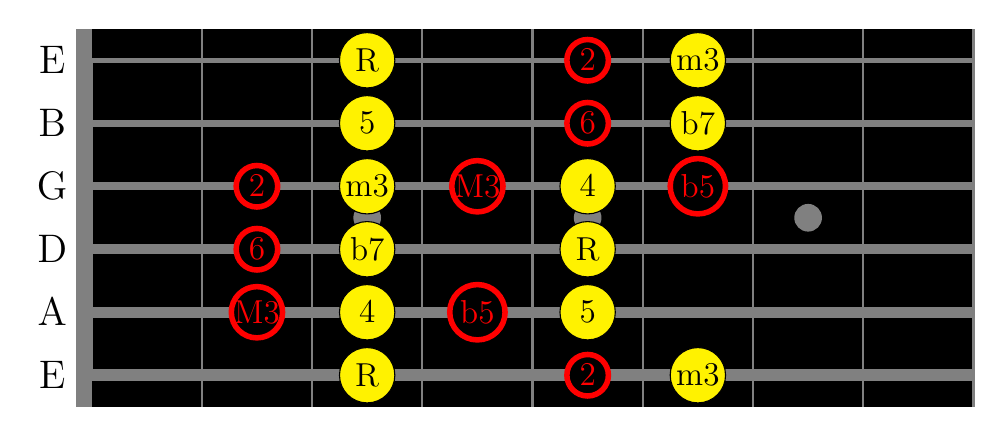
\begin{tikzpicture}[scale=1]
	\def \h{0.8}
	\def \fret{1.4} % 1.6
	\def \L{ 8*\fret }	
	\def \dot_size{5pt}
	\def \circ_size{15pt}
	
	\fill[black, line width=2] (0.0,-0.4) rectangle (8*\fret,4.4);
	\fill[black!50!white, line width=2] (-0.2,-0.4) rectangle (0,4.4);
	
	% Strings
	\draw[color=black!50!white, line width=2.0]  (-0.1, 5*\h) -- (\L,5*\h); % E
	\draw[color=black!50!white, line width=2.5]  (-0.1, 4*\h) -- (\L,4*\h); % B
	\draw[color=black!50!white, line width=3.0]  (-0.1, 3*\h) -- (\L,3*\h); % G
	\draw[color=black!50!white, line width=3.5]  (-0.1, 2*\h) -- (\L,2*\h); % D
	\draw[color=black!50!white, line width=4.0]  (-0.1, 1*\h) -- (\L,1*\h); % A
	\draw[color=black!50!white, line width=4.5]  (-0.1, 0*\h) -- (\L,0*\h); % E
	
	% Frets 0
	\draw[color=black!50!white, thick]  (-0.1, 0) -- (-0.1,5*\h); 
	\draw[color=black!50!white, thick]  (0, 0)   -- (0,5*\h); 
	
	% Fret 1-15
	\draw[color=black!50!white, thick]  (\fret,   -0.4)   -- (\fret,4.4);   
	\draw[color=black!50!white, thick]  (2*\fret, -0.4) -- (2*\fret,4.4); 
	\draw[color=black!50!white, thick]  (3*\fret, -0.4) -- (3*\fret,4.4); 
	\draw[color=black!50!white, thick]  (4*\fret, -0.4) -- (4*\fret,4.4); 
	\draw[color=black!50!white, thick]  (5*\fret, -0.4) -- (5*\fret,4.4); 
	\draw[color=black!50!white, thick]  (6*\fret, -0.4) -- (6*\fret,4.4); 
	\draw[color=black!50!white, thick]  (7*\fret, -0.4) -- (7*\fret,4.4); 
	\draw[color=black!50!white, thick]  (8*\fret, -0.4) -- (8*\fret,4.4); 
%	\draw[color=black!50!white, thick]  (9*\fret, -0.4) -- (9*\fret,4.4); 
%	\draw[color=black!50!white, thick]  (10*\fret, -0.4) -- (10*\fret,4.4); 
%	\draw[color=black!50!white, thick]  (11*\fret, -0.4) -- (11*\fret,4.4); 
%	\draw[color=black!50!white, thick]  (12*\fret, -0.4) -- (12*\fret,4.4); 
%	\draw[color=black!50!white, thick]  (13*\fret, -0.4) -- (13*\fret,4.4); 
%	\draw[color=black!50!white, thick]  (14*\fret, -0.4) -- (14*\fret,4.4); 
%	\draw[color=black!50!white, thick]  (15*\fret, -0.4) -- (15*\fret,4.4); 
%	\draw[color=black!50!white, thick]  (16*\fret, -0.4) -- (16*\fret,4.4); 
%	\draw[color=black!50!white, thick]  (17*\fret, -0.4) -- (17*\fret,4.4); 
%	\draw[color=black!50!white, thick]  (18*\fret, -0.4) -- (18*\fret,4.4); 
%	\draw[color=black!50!white, thick]  (19*\fret, -0.4) -- (19*\fret,4.4); 
%	\draw[color=black!50!white, thick]  (20*\fret, -0.4) -- (20*\fret,4.4); 
	
	% Dots
	\fill[black!50!white] (2.5*\fret,2.5*\h) circle (\dot_size); % fret 3
	\fill[black!50!white] (4.5*\fret,2.5*\h) circle (\dot_size); % fret 5
	\fill[black!50!white] (6.5*\fret,2.5*\h) circle (\dot_size); % fret 7
%	\fill[black!50!white] (8.5*\fret,2.5*\h) circle (\dot_size); % fret 9
%	\fill[black!50!white] (11.5*\fret,1.5*\h) circle (\dot_size); % fret 12
%	\fill[black!50!white] (11.5*\fret,3.5*\h) circle (\dot_size); % fret 12
%	\fill[black!50!white] (14.5*\fret,2.5*\h) circle (\dot_size); % fret 15
%	\fill[black!50!white] (16.5*\fret,2.5*\h) circle (\dot_size); % fret 17
%	\fill[black!50!white] (18.5*\fret,2.5*\h) circle (\dot_size); % fret 19
	
	% String names
	\draw[black] (-0.5,5*\h) node { {\Large E} };
	\draw[black] (-0.5,4*\h) node { {\Large B} };
	\draw[black] (-0.5,3*\h) node { {\Large G} };
	\draw[black] (-0.5,2*\h) node { {\Large D} };
	\draw[black] (-0.5,1*\h) node { {\Large A} };
	\draw[black] (-0.5,0*\h) node { {\Large E} };
	
	% Major scale (fret 1-5)
	\node[dot=\circ_size, draw=red, line width=2,draw] at (4.5*\fret,0) {{\large \textcolor{red}{2}}};
	\node[dot=\circ_size, draw=red, line width=2,draw] at (1.5*\fret,1*\h) {{\large \textcolor{red}{M3}}};
	\node[dot=\circ_size, draw=red, line width=2,draw] at (1.5*\fret,2*\h) {{\large \textcolor{red}{6}}};
	\node[dot=\circ_size, draw=red, line width=2,draw] at (1.5*\fret,3*\h) {{\large \textcolor{red}{2}}};
	\node[dot=\circ_size, draw=red, line width=2,draw] at (3.5*\fret,3*\h) {{\large \textcolor{red}{M3}}};
	\node[dot=\circ_size, draw=red, line width=2,draw] at (4.5*\fret,4*\h) {{\large \textcolor{red}{6}}};
	\node[dot=\circ_size, draw=red, line width=2,draw] at (4.5*\fret,5*\h) {{\large \textcolor{red}{2}}};
	
	\node[dot=20pt, fill=yellow,draw] at (2.5*\fret,0) {{\large \textcolor{black}{R}}};    % Root
	\node[dot=20pt, fill=yellow,draw] at (5.5*\fret,0) {{\large \textcolor{black}{m3}}};    % m3
	\node[dot=20pt, fill=yellow,draw] at (2.5*\fret,1*\h) {{\large \textcolor{black}{4}}};    % 4
	\node[dot=20pt, draw=red, line width=2,draw] at (3.5*\fret,1*\h) {{\large \textcolor{red}{b5}}};
	\node[dot=20pt, fill=yellow,draw] at (4.5*\fret,1*\h) {{\large \textcolor{black}{5}}};
	\node[dot=20pt, fill=yellow,draw] at (2.5*\fret,2*\h) {{\large \textcolor{black}{b7}}};
	\node[dot=20pt, fill=yellow,draw] at (4.5*\fret,2*\h) {{\large \textcolor{black}{R}}};
	\node[dot=20pt, fill=yellow,draw] at (2.5*\fret,3*\h) {{\large \textcolor{black}{m3}}};
	\node[dot=20pt, fill=yellow,draw] at (4.5*\fret,3*\h) {{\large \textcolor{black}{4}}};
	\node[dot=20pt, draw=red, line width=2,draw] at (5.5*\fret,3*\h) {{\large \textcolor{red}{b5}}};
	\node[dot=20pt, fill=yellow,draw] at (2.5*\fret,4*\h) {{\large \textcolor{black}{5}}};
	\node[dot=20pt, fill=yellow,draw] at (5.5*\fret,4*\h) {{\large \textcolor{black}{b7}}};
	\node[dot=20pt, fill=yellow,draw] at (2.5*\fret,5*\h) {{\large \textcolor{black}{R}}};
	\node[dot=20pt, fill=yellow,draw] at (5.5*\fret,5*\h) {{\large \textcolor{black}{m3}}};
	
\end{tikzpicture}
%\end{document}









}
	\caption{(a) Minor pentatonic scale with blue note (b5). (b) Major pentatonic scale. (c) Blues scale  }
	\label{fig:blues_penta_mineur}
\end{figure}

%%%%%%%%%%%%%%%%%%%%%%%%%%%%%%%%%%%%%%%%%%%%%%%%%%%%%%%%%%%%%%%%%%
% Construction of chords superimposing 3rds on a scale
\newpage
\section{Chords}
%%%%%%%%%%%%%%%%%%%%%%%%%%%%%%%%%%%%%%%%%%%%%%%%%%%%%%%%%%%%%%%%%%%%%%%

\begin{itemize}
	\item Tonic: I, iii, vi
	\item Pre-dominant: IV, ii
	\item Dominant: V, vii$^\circ$
\end{itemize}


\begin{itemize}
	\item ``Sus'' chords: chord without third
	\item ``sus9'' will often replace the dominant 7th chord
\end{itemize}

%%%%%%%%%%%%%%%%%%%%%%%%%%%%%%%%%%%%%%%%%%%%%%%%%%%%%%%%%%%%%%%%%%%%%%%%%%%%%%%%%%%%%%%%%%%%%%%%%%%%%%%%%
\newpage
\subsection{Formation of chords}

% Table
% Source: 1997 - Vaillot Méthode Jazz
% Tetrad: https://www.beyondmusictheory.org/chord-formations-triads-and-tetrads/
% Nom de acccords Jake lizzio
\usepackage{arydshln}


\begin{table*}[!h]
	\centering
	\caption{Construction of chords (notation is relative to the major scale)}
	\begin{tabular}{clccclcccl}
		\hline \vspace{-0.2cm} \\
		 & chord & symbol & & & & & & & name \\
		\hline \vspace{-0.2cm} \\
		\multirow{4}{*}{triad} &         & & 1 & M3 & 5           & & & & major\\
		                       & m       & & 1 & m3 & 5           & & & & minor\\
		                       & dim     & $^\circ$ & 1 & m3 & b5     & & & & diminished\\
		                       & aug     & + & 1 & M3 & $^\#$5 & & & & augmented \\
		\hline  \vspace{-0.2cm} \\
		\multirow{4}{*}{ }    & sus2     & & 1 & M2  & 5   &   &   & & suspended 2nd \\
		                       & sus4    & & 1 & 4   & 5   &   &   & & suspended 4th \\
		\hline \vspace{-0.2cm} \\
		\multirow{8}{*}{tetrad}& 7       &                   & 1 & M3  & 5 & m7                & & & dominant 7th \\
		                       & maj7   & $\Delta$, M$7$  & 1 & M3  & 5 & M7  & & & major 7th\\
		                       & m7     & $^{-}$7            & 1 & m3  & 5 & m7  & & & minor 7th\\
		                       & m7b5   & $\varnothing$      & 1 & m3  & b5 & m7 & & & half-diminished \\
		                       & dim7   & $^{\circ}$7        & 1 & m3  & b5 & b7  & & & fully-diminished\\
        					   & mM7    & m$^\Delta$              & 1 & m3  & 5 & M7   & & & minor major 7th \\
							   & maj7($\#$5) & $+^{\Delta}$    & 1 & M3  & $\#$5 & M7  & & & augmented major 7th \\
		                       & 7($\#$5)    & $+^{7}$       & 1 & M3  & $\#$5 & m7  & & & augmented 7th \\
		\hline \vspace{-0.2cm} \\
							   & 6       & & 1 & M3  & 5 & M6   &   & \\
                               & m6      & & 1 & m3  & 5 & M6   &   & \\
							   & b6      & & 1 & M3  & 5 & m6   &   & \\
                               & m(b6)     & & 1 & m3  & 5 & m6   &   & \\
		                       & m6/9   & & 1 & m3  & 6 & M9  &   & \\
		                       & 6/9    & & 1 & M3  & 6 & M9  &   & \\
		                       & add9    & & 1 & M3  & 5 & M9  &   & \\
		  					   & m(add9) & & 1 & m3  & 5 & M9  &   & \\
		\hline  \vspace{-0.2cm} \\
							   & 7sus4   & & 1 & 4   & 5 & m7  &  & \\
		                       & add2    & & 1 & M2  & M3& 5   &  & \\
		\hline
		\multirow{4}{*}{pentad}& 9     & & 1 & M3  & 5 & m7  & M9  & & Dominant 9th \\
	                           & maj9  &$\Delta9$  & 1 & M3  & 5 & M7  & M9  & & major 9th \\
		                       & 7b9 & & 1 & M3  & 5 & m7  & m9  &\\
		                       & m9    & & 1 & m3  & 5 & m7  & M9  & & minor 9th \\
							   & mM9    & & 1 & m3  & 5 & M7  & M9  & & minor major 9th\\
		\hline  \vspace{-0.2cm} \\
		                       & sus9  & & 1 & 4   & 5 & m7  & M9  & \\
		                       & 11    & & 1 & 5   & m7& M9  & 11  & \\ % The 3 is omitted to avoid the dissonace between 3-11.
		\hline
		\multirow{2}{*}{hexad} & 7(13)     & & 1 & M3  & 5 & m7  & M9  & M13\\ % the 11 is omited to avoid the dissonance between 3-11.
		                       & 7(b9,13)  & & 1 & M3  & 5 & m7  & m9  & M13\\
		\hline \vspace{-0.2cm}
	\end{tabular}
	\label{tab: }
\end{table*}

- Accords: 7, m7, maj7, m7b5 (root sur corde E, A, D)

\newpage
\subsection{Harmonizing the major scale}
% Table

\begin{table*}[!h]
	\caption{Harmonization of scales (relative to major scale)}
	\begin{adjustwidth}{0cm}{}
	\begin{tabular}{r|ccc cccc}
		\hline \vspace{-0.4cm} \\
		& 1 & 2 & 3 & 4 & 5 & 6 & 7\\
		\hline \vspace{-0.2cm} \\
		Major  & I$^\Delta$ & ii$^{-7}$ & iii$^{-7 \phantom{\textrm{aug}}$ & IV$^\Delta$ & V$^7$ & vi$^{-7}$ & vii$^{\varnothing}$ \\
		\hline \vspace{-0.2cm} \\
		Natural minor  & i$^{-7}$ & ii$^{\varnothing}$ & bIII$^{\Delta \phantom{\textrm{aug}}}$ & iv$^{-7}$ & v$^{-7}$ & bVI$^{\Delta}$ & bVII$^{7}$ \\
		\hline \vspace{-0.2cm} \\
		Harmonic minor & i$^{\Delta}$ & ii$^{\varnothing}$ & bIII$^{\Delta, \textrm{aug}}$ & iv$^{-7}$ & V$^7$ & bVI$^{\Delta}$ & vii$^{\circ 7}$ \\
		\hline \vspace{-0.2cm} \\
		Melodic minor & i$^{\Delta}$ & ii$^{-7}$ & bIII$^{\Delta, \textrm{aug}}$ & IV$^7$ & V$^7$ & vi$^{\varnothing}$ & vii$^{\varnothing}$ \\
		\hline \vspace{-0.2cm} \\
		Dorian        & i$^{-7}$ & ii$^{-7}$ & bIII$^{\Delta, \phantom{\textrm{aug}}}$ & IV$^{7}$ & v$^{-7}$ & vi$^{\varnothing}$ & bVII$^{\Delta}$ \\
		\hline
	\end{tabular}
	\label{tab: }
	\end{adjustwidth}
\end{table*}

% Table

\begin{table*}[!h]
	\caption{Table of modes }
	\begin{adjustwidth}{-2.3cm}{}
	\begin{tabular}{lccc cccc}
		\hline \vspace{-0.2cm} \\
		Mode name & Ionian & Dorian & Phrygian & Lydian & Mixolydian & Aeolian & Locrian\\
		\hline \vspace{-0.2cm} \\
		Diatonic chords & I & ii$ & iii  & IV & V & vi & vii$^{\circ}$ \\
		Diatonic seventh & $\Delta$7 & $^{-}$7 & $^{-}$7  & $\Delta$7 & 7 & $^{-}$7 & $\varnothing$ \\
		Alternative naming & maj7 & m7 & m7 & maj7 & 7 & m7 & m7b5\\
		%Diatonic seventh  & $\Delta$7 & $^{-}$7 & $^{-}$7 & $\Delta$7 & 7 & $^{-}$7 & $\varnothing$ \\
		\hline \vspace{-0.2cm} \\
		{\scriptsize $\# \# \# \# \# \#$} & F$^\#$ & G$^\#$ & A$^\#$ & B & C$^\#$ & D$^\#$ & E$^\#$ \\
		{\scriptsize $\# \# \# \# \#$}    & B & C$^\#$ & D$^\#$ & E & F$^\#$ & G$^\#$ & A$^\#$\\
		{\scriptsize $\# \# \# \#$}       & E & F$^\#$ & G$^\#$ & A & B & C$^\#$ & D$^\#$\\
		{\scriptsize $\# \# \#$}          & A & B & C$^\#$ & D & E & F$^\#$ & G$^\#$\\
		{\scriptsize $\# \#$}             & D & E & F$^\#$ & G & A & B & C$^\#$\\
		{\scriptsize $\#$}                & G & A & B & C  & D & E & F$^\#$\\
		{\scriptsize -}                   & \textbf{C} & \textbf{D} & \textbf{E} & \textbf{F} & \textbf{G} & \textbf{A} & \textbf{B}\\
		{\scriptsize b}                   & F  & G  & A  & B$^\textrm{b}$ & C  & D  & E\\
		{\scriptsize bb}                  & B$^\textrm{b}$ & C     & D     & E$^\textrm{b}$ & F     & G     & A\\
		{\scriptsize bbb}                 & E$^\textrm{b}$ & F     & G     & A$^\textrm{b}$ & B$^\textrm{b}$ & C     & D\\
		{\scriptsize bbbb}                & A$^\textrm{b}$ & B$^\textrm{b}$ & C     & D$^\textrm{b}$ & E$^\textrm{b}$ & F     & G\\
		{\scriptsize bbbbb}               & D$^\textrm{b}$ & E$^\textrm{b}$ & F     & G$^\textrm{b}$ & A$^\textrm{b}$ & B$^\textrm{b}$ & C\\
		{\scriptsize bbbbbb}              & G$^\textrm{b}$ & A$^\textrm{b}$ & B$^\textrm{b}$ & C$^\textrm{b}$ & D$^\textrm{b}$ & E$^\textrm{b}$ & F\\
		\hline
		\hline \vspace{-0.2cm}
	\end{tabular}
	\label{tab: }
	\end{adjustwidth}
\end{table*}

\newpage
\subsection{Chord progression and example}

% Table
% Source: 1997 - Vaillot Méthode Jazz

\begin{table*}[!h]
	\centering
	\caption{Famous chord progressions}
	\begin{adjustwidth}{-3cm}{}
	\begin{tabular}{p{5.0cm}p{5.5cm}p{7cm}}
		\hline \vspace{-0.2cm} \\
	    Name & Progression & Example\\
		\hline \vspace{-0.2cm} \\
		Pop major (punk)      & $\textrm{I}-\textrm{V}-\textrm{vi}-\textrm{IV}$ & Dammit, Let it be, Country Road \\
		Anatol (turnaround)   & $\textrm{I}^{\Delta}-\textrm{vi}^7-\textrm{ii}^7-\textrm{V}^7$ & Blue Moon \\
		50s progression       & $\textrm{I}-\textrm{vi}-\textrm{IV}-\textrm{V}$ & Every Breath You Take, Crocodile Rock\\
		Ragtime               &$\textrm{I}-\textrm{VI}^7-\textrm{II}^{7}-\textrm{V}^{7}$ & I want to be like you (Disney) \\
		Jazz (ii-V-I)         & $\textrm{ii}^{7}-\textrm{V}^7-\textrm{I}^{\Delta}$ & Autumn leaves\\
		Blues/Rock (Major)    & $\textrm{I}^7-\textrm{IV}^7-\textrm{V}^7-\textrm{I}^7$ & Johnny B. Goode\\

	    Mixo vamp (mixo)      & $\textrm{I}-\textrm{bVII}-\textrm{IV}-\textrm{I}$ & Hey Jude, Sweet home Alabama \\
	    Japanese ``Royal road'' & $\textrm{IV}^\Delta-\textrm{V}^7-\textrm{iii}^7-\textrm{vi}^7-$ {\footnotesize $(\textrm{ii}^7-\textrm{V}^7-\textrm{I}^{\Delta})$} & Shogo theme, anime \\
	    ``Storyteller''       & $\textrm{I}-\textrm{IV}-\textrm{vi}-\textrm{V}$ & \\
	    Creep chord            & I$\,-\,$III$\,-\,$IV$\,-\,$iv &  Creep, Space Oddity \\
		Pop minor             & $\textrm{i}-\textrm{bVI}-\textrm{bIII}-\textrm{bVII}$ & Save Tonight, Africa Toto \\
	    Aeolian vamp          & $\textrm{i}-\textrm{bVII}-\textrm{bVI}-\textrm{bVII}$  & Stairway to Heaven, All Iron Maiden \vspace{-0.8cm}  \\
		Minor progression 01    & $\textrm{i}-\textrm{i}-\textrm{bVI}-\textrm{V}$ & Sweet Dreams \\
	    Minor progression 02    & $\textrm{i}-\textrm{bVI}-\textrm{bIII}-\textrm{bVII}$ &  \\
	    Minor progression 03    & $\textrm{i}-\textrm{bVI}-\textrm{iv}-\textrm{bVII}$ & Final countdown\\
	    Minor progression 04    & $\textrm{i}-\textrm{bIII}-\textrm{bVII}-\textrm{iv}$ & Boulevard of Broken Dreams\\
	    Andalusian	(phrygian)& $\textrm{i}-\textrm{bVII}-\textrm{bVI}-\textrm{V}^7$ & Happy Together The Turtles\\
	    Blues/Rock (minor)      & $\textrm{i}^7-\textrm{iv}^7-\textrm{V}^7-\textrm{i}^7$ & Minor swing\\
	    Anime                   & $\textrm{bVI}-\textrm{bVII}-\textrm{i}$   &             \\
		Neapolitan              & i$\,-\,$bII$^6\,-\,$V$\,-\,$i &  Classic \\
		\hline \vspace{-0.2cm} \\
	\end{tabular}
	\end{adjustwidth}
	\label{tab:}
\end{table*}

%%%%%%%%%%%%%%%%%%%%%%%%%%%%%%%%%%%%%%%%%%%%%%%%%%%%%%%%%%%%%%%%%%%%%%%%%%%%%%%%%%%%%%%%%%%%%%%%%%%%%%%%%
\newpage
\subsection{Chord inversions}

- Accords: 7, m7, maj7, m7b5 (root: E, A, D)

% Figure
\begin{figure}[h!]
	\centering
	\hspace*{-2.2cm}
	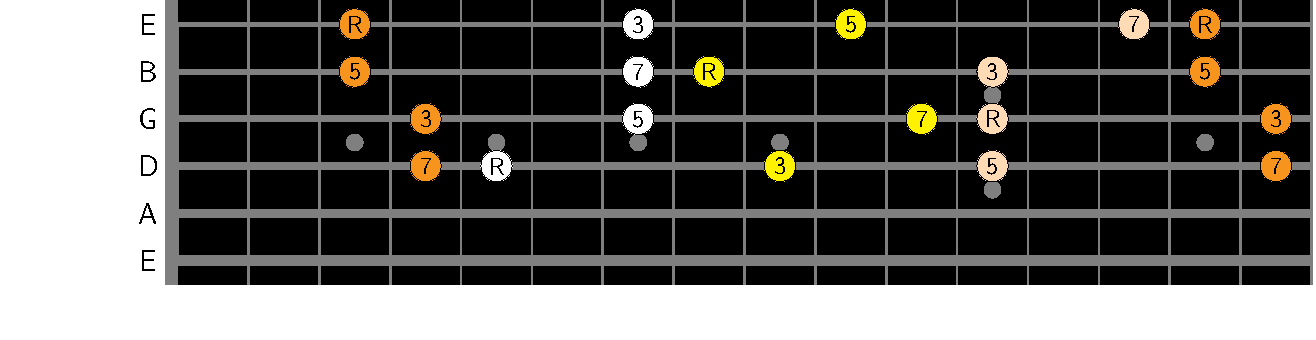
\includegraphics[scale=0.7, trim= {0cm 0cm 0cm 0cm}, clip]{figures/chord-inversions/maj7.pdf}
	\hspace*{-2.2cm}
	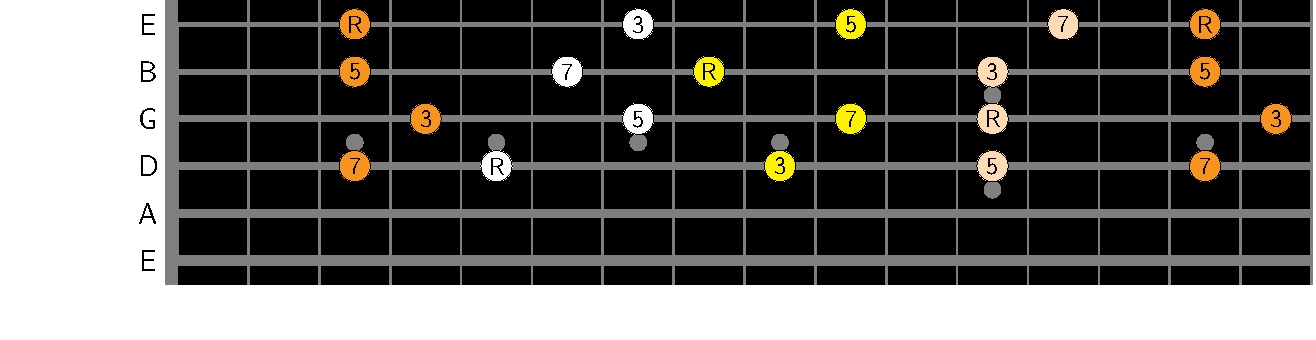
\includegraphics[scale=0.7, trim= {0cm 0cm 0cm 0cm}, clip]{figures/chord-inversions/Dominant7.pdf}
	\hspace*{-2.2cm}
	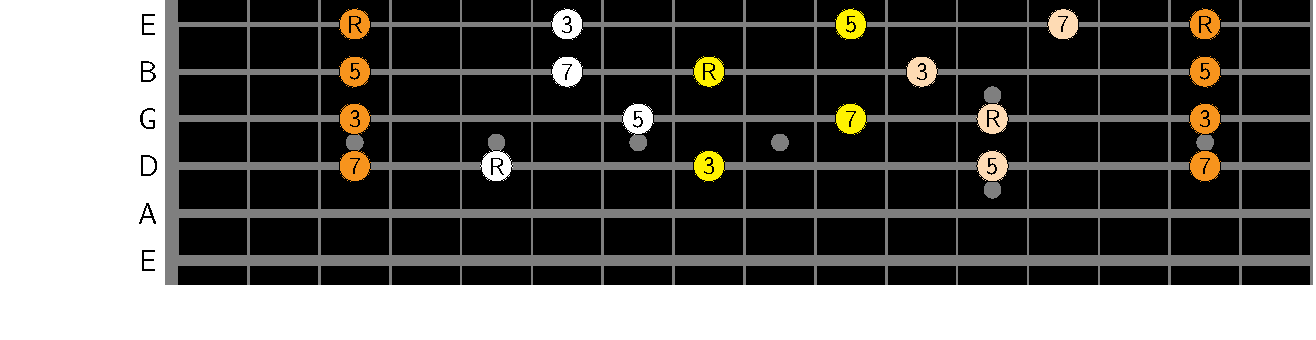
\includegraphics[scale=0.7, trim= {0cm 0cm 0cm 0cm}, clip]{figures/chord-inversions/m7.pdf}
	\caption{(a) maj7 chords. (b) Dominnt 7 chords. (c) m7 chords  }
	\label{fig}
\end{figure}

%%%%%%%%%%%%%%%%%%%%%%%%%%%%%%%%%%%%%%%%%%%%%%%%%%%%%%%%%%%%%%%%%%%%%%%%%%%%%%%%%%%%%%%%%%%%%%%%%%%%%%%%%


Concepts:
\begin{itemize}
	\item Borrowed chord: chord that is not built from the scale of the tonic. Examples:
	\begin{itemize}
		\item ``Picardy third'': a progression with an ending major triad instead of an expected minor triad to create an impression of resolution.
		\item Use the bVII
	\end{itemize}
	\item Transistion Chords:
	\begin{itemize}
		\item Secondary dominant chord (tonicization) (V/x): using the fifth of a chord (even if it's not a diatonic chord) in order to feel a ``resolution'' on this chord.
		\item Tritone substitution (Vsub/x or bV7/V): Approach any target chord with a diminished 7 chord a semitone above.
		\item Backdoor [ii V]. Approach the tonic with iv7 - bVII7 - I.
		\item Modulation (Rick Beato):
		\begin{itemize}
			\item Diatonic common chord (``close'' keys have many chords in common that can be used to modulate from a key to another. Common chords are called pivot chords)
			\item Chromatic pivot chord
			\item Enharmonic dominant
			\item Deceptive
			\item Enharmonic Dim7
			\item Dim7 to Dom7 (lower the root of the dim7 chord to create a dominant chord that leads to a new tonic)
			\item Chromatic Mediant
			\item Common tone (Pivot note)
			\item Direct or Linear (Abrupt change of key without preparation to ``lift'' the song)
			\item Chain Modulation ()
			\item Parallel modulation (Modulation of the mode but keep the same root ex: C to Cm)
		\end{itemize}
	\end{itemize}
\end{itemize}


% Figure
\begin{figure}[h!]
	\centering
	\hspace*{-1cm}
	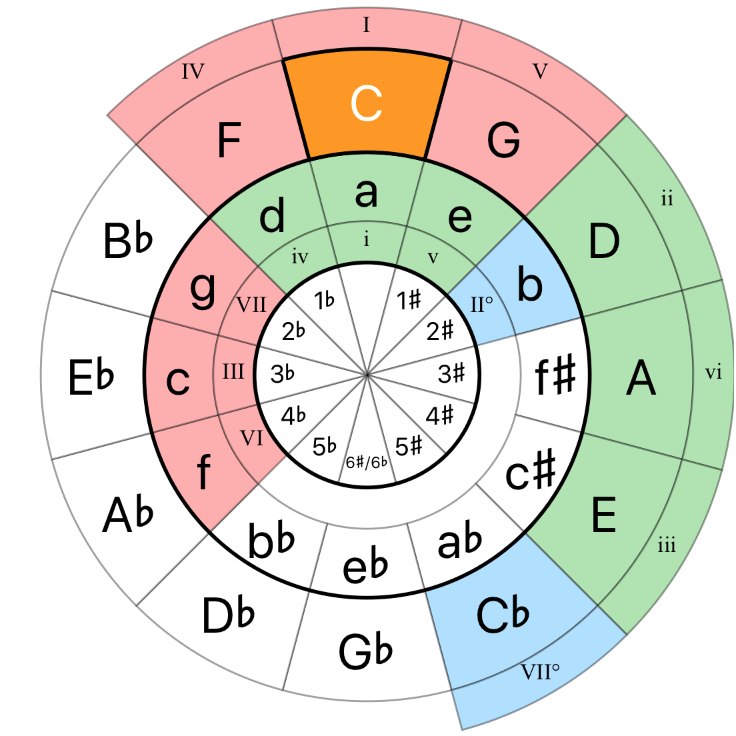
\includegraphics[scale=0.3, trim= {0cm 0cm 0cm 0cm}, clip]{Circle_5th.png}
	\caption{ }
	\label{fig}
\end{figure}

\begin{itemize}
	\item Substitution tritonique
	\item Substitution diatonique
\end{itemize}


%%%%%%%%%%%%%%%%%%%%%%%%%%%%%%%%%%%%%%%%%%%%%%%%%%%%%%%%%%%%%%%%%%
\newpage
\section{Arpeggios}


% Figure
\begin{table}[!h]
	\hspace*{-4.2cm}
	\scalebox{0.52}{

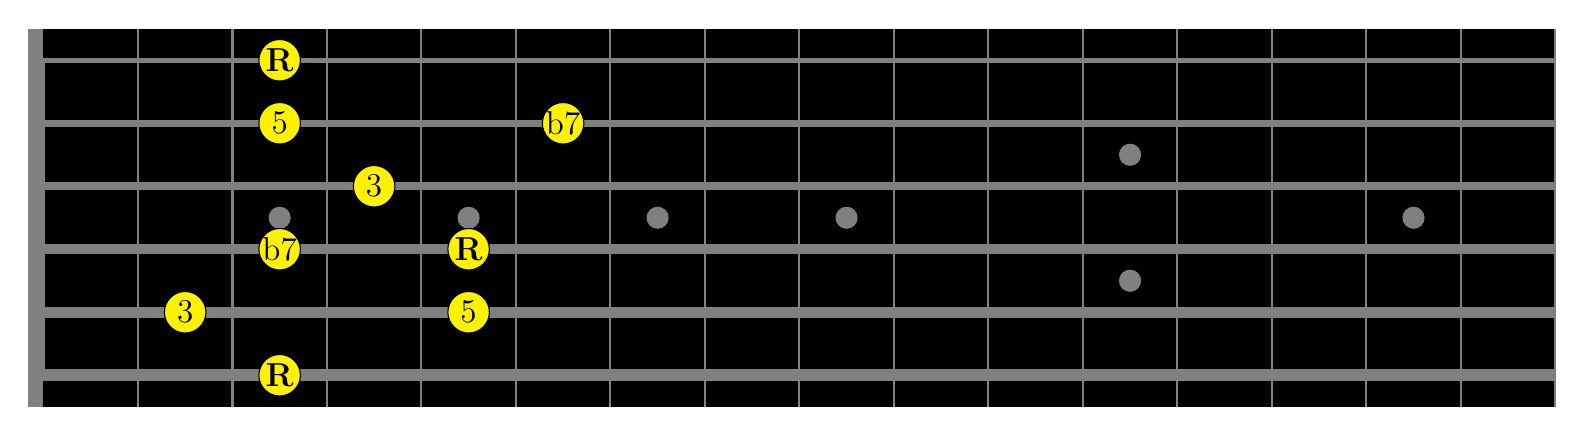
\begin{tikzpicture}[scale=1]
	\def \h{0.8}
	\def \fret{1.2} % 1.6
	\def \L{ 16*\fret }	
	\def \dot_size{4pt}
	\def \circ_size{15pt}
	
	\fill[black, line width=2] (0.0,-0.4) rectangle (16*\fret,4.4);
	\fill[black!50!white, line width=2] (-0.2,-0.4) rectangle (0,4.4);
	
	% Strings
	\draw[color=black!50!white, line width=2.0]  (-0.1, 5*\h) -- (\L,5*\h); % E
	\draw[color=black!50!white, line width=2.5]  (-0.1, 4*\h) -- (\L,4*\h); % B
	\draw[color=black!50!white, line width=3.0]  (-0.1, 3*\h) -- (\L,3*\h); % G
	\draw[color=black!50!white, line width=3.5]  (-0.1, 2*\h) -- (\L,2*\h); % D
	\draw[color=black!50!white, line width=4.0]  (-0.1, 1*\h) -- (\L,1*\h); % A
	\draw[color=black!50!white, line width=4.5]  (-0.1, 0*\h) -- (\L,0*\h); % E
	
	% Frets 0
	\draw[color=black!50!white, thick]  (-0.1, 0) -- (-0.1,5*\h); 
	\draw[color=black!50!white, thick]  (0, 0)   -- (0,5*\h); 
	
	% Fret 1-15
	\draw[color=black!50!white, thick]  (\fret,   -0.4)   -- (\fret,4.4);   
	\draw[color=black!50!white, thick]  (2*\fret, -0.4) -- (2*\fret,4.4); 
	\draw[color=black!50!white, thick]  (3*\fret, -0.4) -- (3*\fret,4.4); 
	\draw[color=black!50!white, thick]  (4*\fret, -0.4) -- (4*\fret,4.4); 
	\draw[color=black!50!white, thick]  (5*\fret, -0.4) -- (5*\fret,4.4); 
	\draw[color=black!50!white, thick]  (6*\fret, -0.4) -- (6*\fret,4.4); 
	\draw[color=black!50!white, thick]  (7*\fret, -0.4) -- (7*\fret,4.4); 
	\draw[color=black!50!white, thick]  (8*\fret, -0.4) -- (8*\fret,4.4); 
	\draw[color=black!50!white, thick]  (9*\fret, -0.4) -- (9*\fret,4.4); 
	\draw[color=black!50!white, thick]  (10*\fret, -0.4) -- (10*\fret,4.4); 
	\draw[color=black!50!white, thick]  (11*\fret, -0.4) -- (11*\fret,4.4); 
	\draw[color=black!50!white, thick]  (12*\fret, -0.4) -- (12*\fret,4.4); 
	\draw[color=black!50!white, thick]  (13*\fret, -0.4) -- (13*\fret,4.4); 
	\draw[color=black!50!white, thick]  (14*\fret, -0.4) -- (14*\fret,4.4); 
	\draw[color=black!50!white, thick]  (15*\fret, -0.4) -- (15*\fret,4.4); 
	\draw[color=black!50!white, thick]  (16*\fret, -0.4) -- (16*\fret,4.4); 
	%\draw[color=black!50!white, thick]  (17*\fret, -0.4) -- (17*\fret,4.4); 
	%\draw[color=black!50!white, thick]  (18*\fret, -0.4) -- (18*\fret,4.4); 
	%\draw[color=black!50!white, thick]  (19*\fret, -0.4) -- (19*\fret,4.4); 
	%\draw[color=black!50!white, thick]  (20*\fret, -0.4) -- (20*\fret,4.4); 
	
	% Dots
	\fill[black!50!white] (2.5*\fret,2.5*\h) circle (\dot_size); % fret 3
	\fill[black!50!white] (4.5*\fret,2.5*\h) circle (\dot_size); % fret 5
	\fill[black!50!white] (6.5*\fret,2.5*\h) circle (\dot_size); % fret 7
	\fill[black!50!white] (8.5*\fret,2.5*\h) circle (\dot_size); % fret 9
	\fill[black!50!white] (11.5*\fret,1.5*\h) circle (\dot_size); % fret 12
	\fill[black!50!white] (11.5*\fret,3.5*\h) circle (\dot_size); % fret 12
	\fill[black!50!white] (14.5*\fret,2.5*\h) circle (\dot_size); % fret 15
	%\fill[black!50!white] (16.5*\fret,2.5*\h) circle (\dot_size); % fret 17
	%\fill[black!50!white] (18.5*\fret,2.5*\h) circle (\dot_size); % fret 19
	
	% String names
%	\draw[black] (-0.5,5*\h) node { {\Large E} };
%	\draw[black] (-0.5,4*\h) node { {\Large B} };
%	\draw[black] (-0.5,3*\h) node { {\Large G} };
%	\draw[black] (-0.5,2*\h) node { {\Large D} };
%	\draw[black] (-0.5,1*\h) node { {\Large A} };
%	\draw[black] (-0.5,0*\h) node { {\Large E} };
	
	% Arpege (position E)
	\node[dot=\circ_size, fill=yellow,draw] at (2.5*\fret,0) {{\large \textbf{R}}};
	\node[dot=\circ_size, fill=yellow,draw] at (1.5*\fret,1*\h) {{\large 3}};
	\node[dot=\circ_size, fill=yellow,draw] at (4.5*\fret,1*\h) {{\large 5}};
	\node[dot=\circ_size, fill=yellow,draw] at (2.5*\fret,2*\h) {{\large b7}};
	\node[dot=\circ_size, fill=yellow,draw] at (4.5*\fret,2*\h) {{\large \textbf{R}}};
	\node[dot=\circ_size, fill=yellow,draw] at (3.5*\fret,3*\h) {{\large 3}};
	\node[dot=\circ_size, fill=yellow,draw] at (2.5*\fret,4*\h) {{\large 5}};
	\node[dot=\circ_size, fill=yellow,draw] at (5.5*\fret,4*\h) {{\large b7}};
	\node[dot=\circ_size, fill=yellow,draw] at (2.5*\fret,5*\h) {{\large \textbf{R}}};


	% Rectangle
%	\draw [draw=yellow!90!black, line width=1.5] (1.9*\fret,-0.5) rectangle (7.2*\fret,4.5);
%	\draw [draw=yellow!50!red!30!white, line width=1.5] (5.8*\fret,+0.4) rectangle (10.2*\fret,4.5);
%	\draw [draw=yellow!50!red!80!white, line width=1.5] (8.9*\fret,+0.2) rectangle (15.1*\fret,4.6);
	
	% Annotation
%	\draw[black,anchor=west] (-3cm,2cm) node { {\Huge 7 } };
	
\end{tikzpicture}




}
	\hspace*{-0cm}
	\scalebox{0.52}{
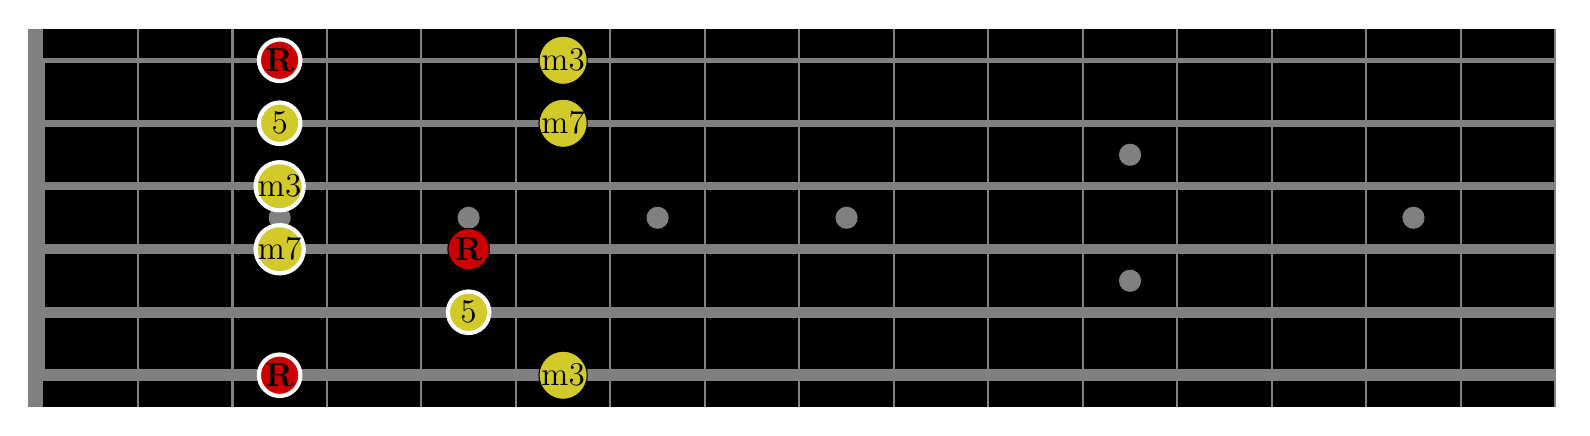
\begin{tikzpicture}[scale=1]
	\def \h{0.8}
	\def \fret{1.2} % 1.6
	\def \L{ 16*\fret }	
	\def \dot_size{4pt}
	\def \circ_size{15pt}
	
	\fill[black, line width=2] (0.0,-0.4) rectangle (16*\fret,4.4);
	\fill[black!50!white, line width=2] (-0.2,-0.4) rectangle (0,4.4);
	
	% Strings
	\draw[color=black!50!white, line width=2.0]  (-0.1, 5*\h) -- (\L,5*\h); % E
	\draw[color=black!50!white, line width=2.5]  (-0.1, 4*\h) -- (\L,4*\h); % B
	\draw[color=black!50!white, line width=3.0]  (-0.1, 3*\h) -- (\L,3*\h); % G
	\draw[color=black!50!white, line width=3.5]  (-0.1, 2*\h) -- (\L,2*\h); % D
	\draw[color=black!50!white, line width=4.0]  (-0.1, 1*\h) -- (\L,1*\h); % A
	\draw[color=black!50!white, line width=4.5]  (-0.1, 0*\h) -- (\L,0*\h); % E
	
	% Frets 0
	\draw[color=black!50!white, thick]  (-0.1, 0) -- (-0.1,5*\h); 
	\draw[color=black!50!white, thick]  (0, 0)   -- (0,5*\h); 
	
	% Fret 1-15
	\draw[color=black!50!white, thick]  (\fret,   -0.4)   -- (\fret,4.4);   
	\draw[color=black!50!white, thick]  (2*\fret, -0.4) -- (2*\fret,4.4); 
	\draw[color=black!50!white, thick]  (3*\fret, -0.4) -- (3*\fret,4.4); 
	\draw[color=black!50!white, thick]  (4*\fret, -0.4) -- (4*\fret,4.4); 
	\draw[color=black!50!white, thick]  (5*\fret, -0.4) -- (5*\fret,4.4); 
	\draw[color=black!50!white, thick]  (6*\fret, -0.4) -- (6*\fret,4.4); 
	\draw[color=black!50!white, thick]  (7*\fret, -0.4) -- (7*\fret,4.4); 
	\draw[color=black!50!white, thick]  (8*\fret, -0.4) -- (8*\fret,4.4); 
	\draw[color=black!50!white, thick]  (9*\fret, -0.4) -- (9*\fret,4.4); 
	\draw[color=black!50!white, thick]  (10*\fret, -0.4) -- (10*\fret,4.4); 
	\draw[color=black!50!white, thick]  (11*\fret, -0.4) -- (11*\fret,4.4); 
	\draw[color=black!50!white, thick]  (12*\fret, -0.4) -- (12*\fret,4.4); 
	\draw[color=black!50!white, thick]  (13*\fret, -0.4) -- (13*\fret,4.4); 
	\draw[color=black!50!white, thick]  (14*\fret, -0.4) -- (14*\fret,4.4); 
	\draw[color=black!50!white, thick]  (15*\fret, -0.4) -- (15*\fret,4.4); 
	\draw[color=black!50!white, thick]  (16*\fret, -0.4) -- (16*\fret,4.4); 
	%\draw[color=black!50!white, thick]  (17*\fret, -0.4) -- (17*\fret,4.4); 
	%\draw[color=black!50!white, thick]  (18*\fret, -0.4) -- (18*\fret,4.4); 
	%\draw[color=black!50!white, thick]  (19*\fret, -0.4) -- (19*\fret,4.4); 
	%\draw[color=black!50!white, thick]  (20*\fret, -0.4) -- (20*\fret,4.4); 
	
	% Dots
	\fill[black!50!white] (2.5*\fret,2.5*\h) circle (\dot_size); % fret 3
	\fill[black!50!white] (4.5*\fret,2.5*\h) circle (\dot_size); % fret 5
	\fill[black!50!white] (6.5*\fret,2.5*\h) circle (\dot_size); % fret 7
	\fill[black!50!white] (8.5*\fret,2.5*\h) circle (\dot_size); % fret 9
	\fill[black!50!white] (11.5*\fret,1.5*\h) circle (\dot_size); % fret 12
	\fill[black!50!white] (11.5*\fret,3.5*\h) circle (\dot_size); % fret 12
	\fill[black!50!white] (14.5*\fret,2.5*\h) circle (\dot_size); % fret 15
	%\fill[black!50!white] (16.5*\fret,2.5*\h) circle (\dot_size); % fret 17
	%\fill[black!50!white] (18.5*\fret,2.5*\h) circle (\dot_size); % fret 19
	
	% String names
%	\draw[black] (-0.5,5*\h) node { {\Large E} };
%	\draw[black] (-0.5,4*\h) node { {\Large B} };
%	\draw[black] (-0.5,3*\h) node { {\Large G} };
%	\draw[black] (-0.5,2*\h) node { {\Large D} };
%	\draw[black] (-0.5,1*\h) node { {\Large A} };
%	\draw[black] (-0.5,0*\h) node { {\Large E} };
	
	% Arpege (position A)
	\node[dot=\circ_size, fill=red!80!black,draw=white, line width=1.5pt] at (2.5*\fret,0) {{\large \textbf{R}}};
	\node[dot=\circ_size, fill=yellow!80!black,draw] at (5.5*\fret,0) {{\large m3}};
	\node[dot=\circ_size, fill=yellow!80!black,draw=white, line width=1.5pt] at (4.5*\fret,1*\h) {{\large 5}};
	\node[dot=\circ_size, fill=yellow!80!black,draw=white, line width=1.5pt] at (2.5*\fret,2*\h) {{\large m7}};
	\node[dot=\circ_size, fill=red!80!black,draw] at (4.5*\fret,2*\h) {{\large \textbf{R}}};
	\node[dot=\circ_size, fill=yellow!80!black,draw=white, line width=1.5pt] at (2.5*\fret,3*\h) {{\large m3}};
	\node[dot=\circ_size, fill=yellow!80!black,draw=white, line width=1.5pt] at (2.5*\fret,4*\h) {{\large 5}};
	\node[dot=\circ_size, fill=yellow!80!black,draw] at (5.5*\fret,4*\h) {{\large m7}};
	\node[dot=\circ_size, fill=red!80!black,draw=white, line width=1.5pt] at (2.5*\fret,5*\h) {{\large \textbf{R}}};
	\node[dot=\circ_size, fill=yellow!80!black,draw] at (5.5*\fret,5*\h) {{\large m3}};
	
	% Arpege (position G-E)
%	\node[dot=\circ_size, fill=yellow!50!red!30!white,draw] at (5.5*\fret,0*\h) {{\normalsize m3}};
%	\node[dot=\circ_size, fill=yellow!50!red!30!white,draw] at (9.5*\fret,0*\h) {{\large 5}};
%	\node[dot=\circ_size, fill=white,draw] at (7.5*\fret,1*\h) {{\large b7}};
%	\node[dot=\circ_size, fill=yellow!50!red!30!white,draw] at (9.5*\fret,1*\h) {{\large R}};
%	\node[dot=\circ_size, fill=yellow!50!red!30!white,draw] at (7.5*\fret,2*\h) {{\normalsize m3}};
%	\node[dot=\circ_size, fill=yellow!50!red!30!white,draw] at (6.5*\fret,3*\h) {{\large 5}};
%	\node[dot=\circ_size, fill=white,draw] at (5.5*\fret,4*\h) {{\large b7}};
%	\node[dot=\circ_size, fill=yellow!50!red!30!white,draw] at (7.5*\fret,4*\h) {{\large R}};
%	\node[dot=\circ_size, fill=yellow!50!red!30!white,draw] at (5.5*\fret,5*\h) {{\normalsize m3}};
%	\node[dot=\circ_size, fill=yellow!50!red!30!white,draw] at (9.5*\fret,5*\h) {{\large 5}};
%
%	% Arpege (position D-C)
%	\node[dot=\circ_size, fill=yellow!50!red!80!white,draw] at (12.5*\fret,1*\h) {{\normalsize m3}};
%	\node[dot=\circ_size, fill=yellow!50!red!80!white,draw] at (11.5*\fret,2*\h) {{\large 5}};
%	\node[dot=\circ_size, fill=white,draw] at (9.5*\fret,3*\h) {{\large b7}};
%	\node[dot=\circ_size, fill=yellow!50!red!80!white,draw] at (11.5*\fret,3*\h) {{\large R}};
%	\node[dot=\circ_size, fill=yellow!50!red!80!white,draw] at (10.5*\fret,4*\h) {{\normalsize m3}};
%	\node[dot=\circ_size, fill=white,draw] at (12.5*\fret,5*\h) {{\large b7}};
	
	% Anotation (positions)
%	\draw[black,anchor=center, text width=3.5cm, align=center] (6,-1) node { {\Large \textbf{A pos.} }};
%	\draw[black,anchor=center, text width=3.5cm, align=center] (9,-1) node { {\Large \textbf{G-E pos.} }};
%	\draw[black,anchor=center, text width=3.5cm, align=center] (14,-1) node { {\Large \textbf{D-C pos.} }};
%
%	% Rectangle
%	\draw [draw=yellow!90!black, line width=1.5] (0.8*\fret,0.4) rectangle (6.1*\fret,4.6);
%	\draw [draw=yellow!50!red!30!white, line width=1.5] (4.8*\fret,-0.5) rectangle (10.2*\fret,4.5);
%	\draw [draw=yellow!50!red!80!white, line width=1.5] (8.9*\fret,+0.2) rectangle (14.2*\fret,4.6);
%
%	% Annotation
%	\draw[black,anchor=west] (-3cm,2cm) node { {\Huge m7 } };
	
\end{tikzpicture}
%\end{document}




}

	\hspace*{-4.2cm}
	\scalebox{0.52}{

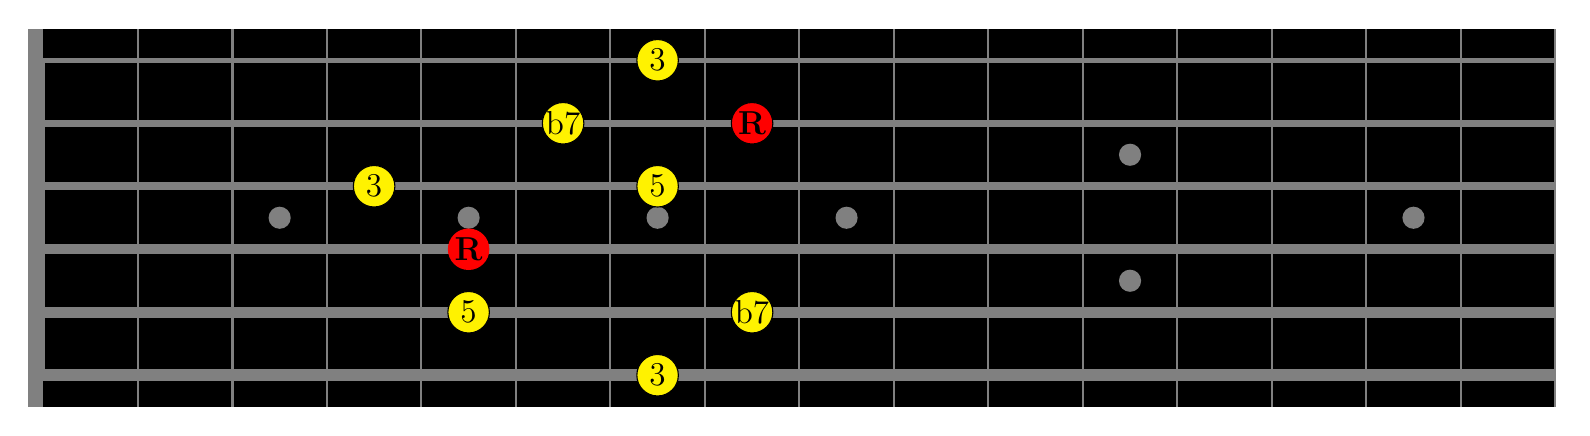
\begin{tikzpicture}[scale=1]
	\def \h{0.8}
	\def \fret{1.2} % 1.6
	\def \L{ 16*\fret }	
	\def \dot_size{4pt}
	\def \circ_size{15pt}
	
	\fill[black, line width=2] (0.0,-0.4) rectangle (16*\fret,4.4);
	\fill[black!50!white, line width=2] (-0.2,-0.4) rectangle (0,4.4);
	
	% Strings
	\draw[color=black!50!white, line width=2.0]  (-0.1, 5*\h) -- (\L,5*\h); % E
	\draw[color=black!50!white, line width=2.5]  (-0.1, 4*\h) -- (\L,4*\h); % B
	\draw[color=black!50!white, line width=3.0]  (-0.1, 3*\h) -- (\L,3*\h); % G
	\draw[color=black!50!white, line width=3.5]  (-0.1, 2*\h) -- (\L,2*\h); % D
	\draw[color=black!50!white, line width=4.0]  (-0.1, 1*\h) -- (\L,1*\h); % A
	\draw[color=black!50!white, line width=4.5]  (-0.1, 0*\h) -- (\L,0*\h); % E
	
	% Frets 0
	\draw[color=black!50!white, thick]  (-0.1, 0) -- (-0.1,5*\h); 
	\draw[color=black!50!white, thick]  (0, 0)   -- (0,5*\h); 
	
	% Fret 1-15
	\draw[color=black!50!white, thick]  (\fret,   -0.4)   -- (\fret,4.4);   
	\draw[color=black!50!white, thick]  (2*\fret, -0.4) -- (2*\fret,4.4); 
	\draw[color=black!50!white, thick]  (3*\fret, -0.4) -- (3*\fret,4.4); 
	\draw[color=black!50!white, thick]  (4*\fret, -0.4) -- (4*\fret,4.4); 
	\draw[color=black!50!white, thick]  (5*\fret, -0.4) -- (5*\fret,4.4); 
	\draw[color=black!50!white, thick]  (6*\fret, -0.4) -- (6*\fret,4.4); 
	\draw[color=black!50!white, thick]  (7*\fret, -0.4) -- (7*\fret,4.4); 
	\draw[color=black!50!white, thick]  (8*\fret, -0.4) -- (8*\fret,4.4); 
	\draw[color=black!50!white, thick]  (9*\fret, -0.4) -- (9*\fret,4.4); 
	\draw[color=black!50!white, thick]  (10*\fret, -0.4) -- (10*\fret,4.4); 
	\draw[color=black!50!white, thick]  (11*\fret, -0.4) -- (11*\fret,4.4); 
	\draw[color=black!50!white, thick]  (12*\fret, -0.4) -- (12*\fret,4.4); 
	\draw[color=black!50!white, thick]  (13*\fret, -0.4) -- (13*\fret,4.4); 
	\draw[color=black!50!white, thick]  (14*\fret, -0.4) -- (14*\fret,4.4); 
	\draw[color=black!50!white, thick]  (15*\fret, -0.4) -- (15*\fret,4.4); 
	\draw[color=black!50!white, thick]  (16*\fret, -0.4) -- (16*\fret,4.4); 
	%\draw[color=black!50!white, thick]  (17*\fret, -0.4) -- (17*\fret,4.4); 
	%\draw[color=black!50!white, thick]  (18*\fret, -0.4) -- (18*\fret,4.4); 
	%\draw[color=black!50!white, thick]  (19*\fret, -0.4) -- (19*\fret,4.4); 
	%\draw[color=black!50!white, thick]  (20*\fret, -0.4) -- (20*\fret,4.4); 
	
	% Dots
	\fill[black!50!white] (2.5*\fret,2.5*\h) circle (\dot_size); % fret 3
	\fill[black!50!white] (4.5*\fret,2.5*\h) circle (\dot_size); % fret 5
	\fill[black!50!white] (6.5*\fret,2.5*\h) circle (\dot_size); % fret 7
	\fill[black!50!white] (8.5*\fret,2.5*\h) circle (\dot_size); % fret 9
	\fill[black!50!white] (11.5*\fret,1.5*\h) circle (\dot_size); % fret 12
	\fill[black!50!white] (11.5*\fret,3.5*\h) circle (\dot_size); % fret 12
	\fill[black!50!white] (14.5*\fret,2.5*\h) circle (\dot_size); % fret 15
	%\fill[black!50!white] (16.5*\fret,2.5*\h) circle (\dot_size); % fret 17
	%\fill[black!50!white] (18.5*\fret,2.5*\h) circle (\dot_size); % fret 19
	
	% String names
%	\draw[black] (-0.5,5*\h) node { {\Large E} };
%	\draw[black] (-0.5,4*\h) node { {\Large B} };
%	\draw[black] (-0.5,3*\h) node { {\Large G} };
%	\draw[black] (-0.5,2*\h) node { {\Large D} };
%	\draw[black] (-0.5,1*\h) node { {\Large A} };
%	\draw[black] (-0.5,0*\h) node { {\Large E} };

	% Arpege (position D-C)
    \node[dot=\circ_size, fill=yellow,draw] at (6.5*\fret,0*\h) {{\large 3}};
	\node[dot=\circ_size, fill=yellow,draw] at (7.5*\fret,1*\h) {{\large b7}};
	\node[dot=\circ_size, fill=yellow,draw] at (4.5*\fret,1*\h) {{\large 5}};
	\node[dot=\circ_size, fill=red] at (4.5*\fret,2*\h) {{\large \textbf{R}}};
	\node[dot=\circ_size, fill=yellow,draw] at (3.5*\fret,3*\h) {{\large 3}};
	\node[dot=\circ_size, fill=yellow,draw] at (6.5*\fret,3*\h) {{\large 5}};
	\node[dot=\circ_size, fill=yellow,draw] at (5.5*\fret,4*\h) {{\large b7}};
	\node[dot=\circ_size,  fill=red,draw] at (7.5*\fret,4*\h) {{\large \textbf{R}}};
	\node[dot=\circ_size, fill=yellow,draw] at (6.5*\fret,5*\h) {{\large 3}};
%
	% Rectangle
%	\draw [draw=yellow!90!black, line width=1.5] (1.9*\fret,-0.5) rectangle (7.2*\fret,4.5);
%	\draw [draw=yellow!50!red!30!white, line width=1.5] (5.8*\fret,+0.4) rectangle (10.2*\fret,4.5);
%	\draw [draw=yellow!50!red!80!white, line width=1.5] (8.9*\fret,+0.2) rectangle (15.1*\fret,4.6);
	
	% Annotation
%	\draw[black,anchor=west] (-3cm,2cm) node { {\Huge 7 } };
	
\end{tikzpicture}




}
	\hspace*{-0cm}
	\scalebox{0.52}{
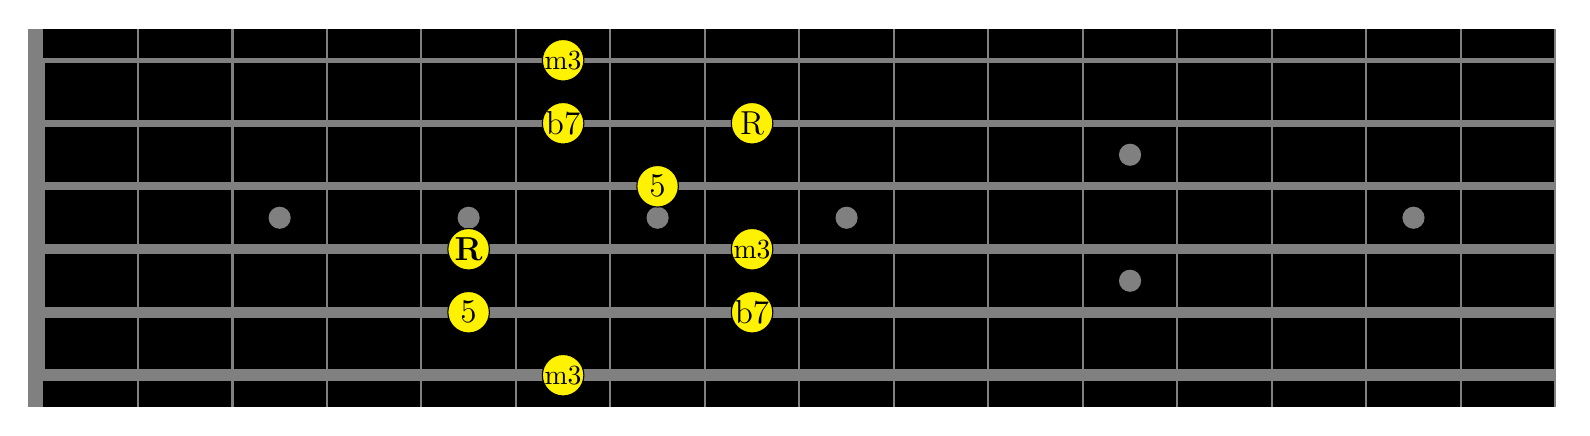
\begin{tikzpicture}[scale=1]
	\def \h{0.8}
	\def \fret{1.2} % 1.6
	\def \L{ 16*\fret }	
	\def \dot_size{4pt}
	\def \circ_size{15pt}
	
	\fill[black, line width=2] (0.0,-0.4) rectangle (16*\fret,4.4);
	\fill[black!50!white, line width=2] (-0.2,-0.4) rectangle (0,4.4);
	
	% Strings
	\draw[color=black!50!white, line width=2.0]  (-0.1, 5*\h) -- (\L,5*\h); % E
	\draw[color=black!50!white, line width=2.5]  (-0.1, 4*\h) -- (\L,4*\h); % B
	\draw[color=black!50!white, line width=3.0]  (-0.1, 3*\h) -- (\L,3*\h); % G
	\draw[color=black!50!white, line width=3.5]  (-0.1, 2*\h) -- (\L,2*\h); % D
	\draw[color=black!50!white, line width=4.0]  (-0.1, 1*\h) -- (\L,1*\h); % A
	\draw[color=black!50!white, line width=4.5]  (-0.1, 0*\h) -- (\L,0*\h); % E
	
	% Frets 0
	\draw[color=black!50!white, thick]  (-0.1, 0) -- (-0.1,5*\h); 
	\draw[color=black!50!white, thick]  (0, 0)   -- (0,5*\h); 
	
	% Fret 1-15
	\draw[color=black!50!white, thick]  (\fret,   -0.4)   -- (\fret,4.4);   
	\draw[color=black!50!white, thick]  (2*\fret, -0.4) -- (2*\fret,4.4); 
	\draw[color=black!50!white, thick]  (3*\fret, -0.4) -- (3*\fret,4.4); 
	\draw[color=black!50!white, thick]  (4*\fret, -0.4) -- (4*\fret,4.4); 
	\draw[color=black!50!white, thick]  (5*\fret, -0.4) -- (5*\fret,4.4); 
	\draw[color=black!50!white, thick]  (6*\fret, -0.4) -- (6*\fret,4.4); 
	\draw[color=black!50!white, thick]  (7*\fret, -0.4) -- (7*\fret,4.4); 
	\draw[color=black!50!white, thick]  (8*\fret, -0.4) -- (8*\fret,4.4); 
	\draw[color=black!50!white, thick]  (9*\fret, -0.4) -- (9*\fret,4.4); 
	\draw[color=black!50!white, thick]  (10*\fret, -0.4) -- (10*\fret,4.4); 
	\draw[color=black!50!white, thick]  (11*\fret, -0.4) -- (11*\fret,4.4); 
	\draw[color=black!50!white, thick]  (12*\fret, -0.4) -- (12*\fret,4.4); 
	\draw[color=black!50!white, thick]  (13*\fret, -0.4) -- (13*\fret,4.4); 
	\draw[color=black!50!white, thick]  (14*\fret, -0.4) -- (14*\fret,4.4); 
	\draw[color=black!50!white, thick]  (15*\fret, -0.4) -- (15*\fret,4.4); 
	\draw[color=black!50!white, thick]  (16*\fret, -0.4) -- (16*\fret,4.4); 
	%\draw[color=black!50!white, thick]  (17*\fret, -0.4) -- (17*\fret,4.4); 
	%\draw[color=black!50!white, thick]  (18*\fret, -0.4) -- (18*\fret,4.4); 
	%\draw[color=black!50!white, thick]  (19*\fret, -0.4) -- (19*\fret,4.4); 
	%\draw[color=black!50!white, thick]  (20*\fret, -0.4) -- (20*\fret,4.4); 
	
	% Dots
	\fill[black!50!white] (2.5*\fret,2.5*\h) circle (\dot_size); % fret 3
	\fill[black!50!white] (4.5*\fret,2.5*\h) circle (\dot_size); % fret 5
	\fill[black!50!white] (6.5*\fret,2.5*\h) circle (\dot_size); % fret 7
	\fill[black!50!white] (8.5*\fret,2.5*\h) circle (\dot_size); % fret 9
	\fill[black!50!white] (11.5*\fret,1.5*\h) circle (\dot_size); % fret 12
	\fill[black!50!white] (11.5*\fret,3.5*\h) circle (\dot_size); % fret 12
	\fill[black!50!white] (14.5*\fret,2.5*\h) circle (\dot_size); % fret 15
	%\fill[black!50!white] (16.5*\fret,2.5*\h) circle (\dot_size); % fret 17
	%\fill[black!50!white] (18.5*\fret,2.5*\h) circle (\dot_size); % fret 19
	
	% String names
%	\draw[black] (-0.5,5*\h) node { {\Large E} };
%	\draw[black] (-0.5,4*\h) node { {\Large B} };
%	\draw[black] (-0.5,3*\h) node { {\Large G} };
%	\draw[black] (-0.5,2*\h) node { {\Large D} };
%	\draw[black] (-0.5,1*\h) node { {\Large A} };
%	\draw[black] (-0.5,0*\h) node { {\Large E} };
	
	% Arpege (position A)
%	\node[dot=\circ_size, fill=yellow,draw] at (2.5*\fret,0) {{\large \textbf{R}}};
%	\node[dot=\circ_size, fill=yellow,draw] at (5.5*\fret,0) {{\large \textbf{m3}}};
%	\node[dot=\circ_size, fill=yellow,draw] at (4.5*\fret,1*\h) {{\large 5}};
%	\node[dot=\circ_size, fill=yellow,draw] at (2.5*\fret,2*\h) {{\large b7}};
%	\node[dot=\circ_size, fill=yellow,draw] at (4.5*\fret,2*\h) {{\large \textbf{R}}};
%	\node[dot=\circ_size, fill=yellow,draw] at (2.5*\fret,3*\h) {{\large m3}};
%	\node[dot=\circ_size, fill=yellow,draw] at (2.5*\fret,4*\h) {{\large 5}};
%	\node[dot=\circ_size, fill=yellow,draw] at (5.5*\fret,4*\h) {{\large b7}};
%	\node[dot=\circ_size, fill=yellow,draw] at (2.5*\fret,5*\h) {{\large \textbf{R}}};
%	\node[dot=\circ_size, fill=yellow,draw] at (5.5*\fret,5*\h) {{\large m3}};
	
	% Arpege (position G-E)
	\node[dot=\circ_size, fill=yellow,draw] at (5.5*\fret,0*\h) {{\normalsize m3}};
	\node[dot=\circ_size, fill=yellow,draw] at (4.5*\fret,1*\h) {{\large 5}};
	\node[dot=\circ_size, fill=yellow,draw] at (7.5*\fret,1*\h) {{\large b7}};
	\node[dot=\circ_size, fill=yellow,draw] at (4.5*\fret,2*\h) {{\large \textbf{R}}};
	\node[dot=\circ_size, fill=yellow,draw] at (7.5*\fret,2*\h) {{\normalsize m3}};
	\node[dot=\circ_size, fill=yellow,draw] at (6.5*\fret,3*\h) {{\large 5}};
	\node[dot=\circ_size, fill=yellow,draw] at (5.5*\fret,4*\h) {{\large b7}};
	\node[dot=\circ_size, fill=yellow,draw] at (7.5*\fret,4*\h) {{\large R}};
	\node[dot=\circ_size, fill=yellow,draw] at (5.5*\fret,5*\h) {{\normalsize m3}};
%
%	% Arpege (position D-C)
%	\node[dot=\circ_size, fill=yellow!50!red!80!white,draw] at (12.5*\fret,1*\h) {{\normalsize m3}};
%	\node[dot=\circ_size, fill=yellow!50!red!80!white,draw] at (11.5*\fret,2*\h) {{\large 5}};
%	\node[dot=\circ_size, fill=white,draw] at (9.5*\fret,3*\h) {{\large b7}};
%	\node[dot=\circ_size, fill=yellow!50!red!80!white,draw] at (11.5*\fret,3*\h) {{\large R}};
%	\node[dot=\circ_size, fill=yellow!50!red!80!white,draw] at (10.5*\fret,4*\h) {{\normalsize m3}};
%	\node[dot=\circ_size, fill=white,draw] at (12.5*\fret,5*\h) {{\large b7}};
	
	% Anotation (positions)
%	\draw[black,anchor=center, text width=3.5cm, align=center] (6,-1) node { {\Large \textbf{A pos.} }};
%	\draw[black,anchor=center, text width=3.5cm, align=center] (9,-1) node { {\Large \textbf{G-E pos.} }};
%	\draw[black,anchor=center, text width=3.5cm, align=center] (14,-1) node { {\Large \textbf{D-C pos.} }};
%
%	% Rectangle
%	\draw [draw=yellow!90!black, line width=1.5] (0.8*\fret,0.4) rectangle (6.1*\fret,4.6);
%	\draw [draw=yellow!50!red!30!white, line width=1.5] (4.8*\fret,-0.5) rectangle (10.2*\fret,4.5);
%	\draw [draw=yellow!50!red!80!white, line width=1.5] (8.9*\fret,+0.2) rectangle (14.2*\fret,4.6);
%
%	% Annotation
%	\draw[black,anchor=west] (-3cm,2cm) node { {\Huge m7 } };
	
\end{tikzpicture}
%\end{document}




}

	\hspace*{-4.2cm}
	\scalebox{0.52}{

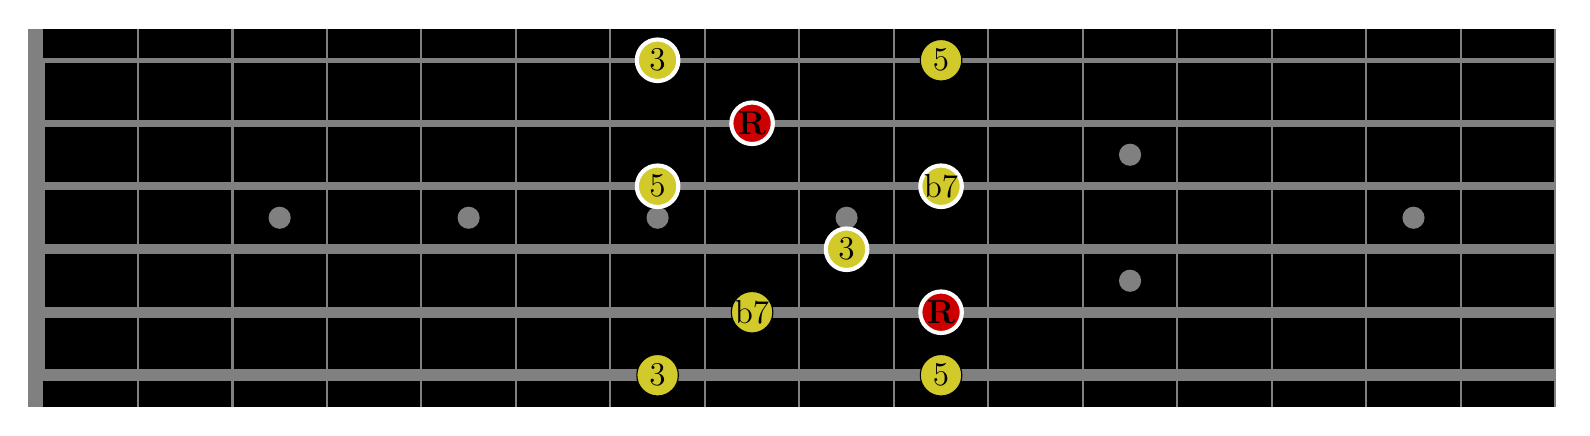
\begin{tikzpicture}[scale=1]
	\def \h{0.8}
	\def \fret{1.2} % 1.6
	\def \L{ 16*\fret }	
	\def \dot_size{4pt}
	\def \circ_size{15pt}
	
	\fill[black, line width=2] (0.0,-0.4) rectangle (16*\fret,4.4);
	\fill[black!50!white, line width=2] (-0.2,-0.4) rectangle (0,4.4);
	
	% Strings
	\draw[color=black!50!white, line width=2.0]  (-0.1, 5*\h) -- (\L,5*\h); % E
	\draw[color=black!50!white, line width=2.5]  (-0.1, 4*\h) -- (\L,4*\h); % B
	\draw[color=black!50!white, line width=3.0]  (-0.1, 3*\h) -- (\L,3*\h); % G
	\draw[color=black!50!white, line width=3.5]  (-0.1, 2*\h) -- (\L,2*\h); % D
	\draw[color=black!50!white, line width=4.0]  (-0.1, 1*\h) -- (\L,1*\h); % A
	\draw[color=black!50!white, line width=4.5]  (-0.1, 0*\h) -- (\L,0*\h); % E
	
	% Frets 0
	\draw[color=black!50!white, thick]  (-0.1, 0) -- (-0.1,5*\h); 
	\draw[color=black!50!white, thick]  (0, 0)   -- (0,5*\h); 
	
	% Fret 1-15
	\draw[color=black!50!white, thick]  (\fret,   -0.4)   -- (\fret,4.4);   
	\draw[color=black!50!white, thick]  (2*\fret, -0.4) -- (2*\fret,4.4); 
	\draw[color=black!50!white, thick]  (3*\fret, -0.4) -- (3*\fret,4.4); 
	\draw[color=black!50!white, thick]  (4*\fret, -0.4) -- (4*\fret,4.4); 
	\draw[color=black!50!white, thick]  (5*\fret, -0.4) -- (5*\fret,4.4); 
	\draw[color=black!50!white, thick]  (6*\fret, -0.4) -- (6*\fret,4.4); 
	\draw[color=black!50!white, thick]  (7*\fret, -0.4) -- (7*\fret,4.4); 
	\draw[color=black!50!white, thick]  (8*\fret, -0.4) -- (8*\fret,4.4); 
	\draw[color=black!50!white, thick]  (9*\fret, -0.4) -- (9*\fret,4.4); 
	\draw[color=black!50!white, thick]  (10*\fret, -0.4) -- (10*\fret,4.4); 
	\draw[color=black!50!white, thick]  (11*\fret, -0.4) -- (11*\fret,4.4); 
	\draw[color=black!50!white, thick]  (12*\fret, -0.4) -- (12*\fret,4.4); 
	\draw[color=black!50!white, thick]  (13*\fret, -0.4) -- (13*\fret,4.4); 
	\draw[color=black!50!white, thick]  (14*\fret, -0.4) -- (14*\fret,4.4); 
	\draw[color=black!50!white, thick]  (15*\fret, -0.4) -- (15*\fret,4.4); 
	\draw[color=black!50!white, thick]  (16*\fret, -0.4) -- (16*\fret,4.4); 
	%\draw[color=black!50!white, thick]  (17*\fret, -0.4) -- (17*\fret,4.4); 
	%\draw[color=black!50!white, thick]  (18*\fret, -0.4) -- (18*\fret,4.4); 
	%\draw[color=black!50!white, thick]  (19*\fret, -0.4) -- (19*\fret,4.4); 
	%\draw[color=black!50!white, thick]  (20*\fret, -0.4) -- (20*\fret,4.4); 
	
	% Dots
	\fill[black!50!white] (2.5*\fret,2.5*\h) circle (\dot_size); % fret 3
	\fill[black!50!white] (4.5*\fret,2.5*\h) circle (\dot_size); % fret 5
	\fill[black!50!white] (6.5*\fret,2.5*\h) circle (\dot_size); % fret 7
	\fill[black!50!white] (8.5*\fret,2.5*\h) circle (\dot_size); % fret 9
	\fill[black!50!white] (11.5*\fret,1.5*\h) circle (\dot_size); % fret 12
	\fill[black!50!white] (11.5*\fret,3.5*\h) circle (\dot_size); % fret 12
	\fill[black!50!white] (14.5*\fret,2.5*\h) circle (\dot_size); % fret 15
	%\fill[black!50!white] (16.5*\fret,2.5*\h) circle (\dot_size); % fret 17
	%\fill[black!50!white] (18.5*\fret,2.5*\h) circle (\dot_size); % fret 19
	
	% String names
%	\draw[black] (-0.5,5*\h) node { {\Large E} };
%	\draw[black] (-0.5,4*\h) node { {\Large B} };
%	\draw[black] (-0.5,3*\h) node { {\Large G} };
%	\draw[black] (-0.5,2*\h) node { {\Large D} };
%	\draw[black] (-0.5,1*\h) node { {\Large A} };
%	\draw[black] (-0.5,0*\h) node { {\Large E} };

	% Notes position
    \node[dot=\circ_size, fill=yellow!80!black,draw] at (6.5*\fret,0*\h) {{\large 3}};
	\node[dot=\circ_size, fill=yellow!80!black,draw] at (9.5*\fret,0*\h) {{\large 5}};
	\node[dot=\circ_size, fill=yellow!80!black,draw] at (7.5*\fret,1*\h) {{\large b7}};
	\node[dot=\circ_size, fill=red!80!black,draw=white, line width=1.5pt] at (9.5*\fret,1*\h) {{\large \textbf{R}}};
	\node[dot=\circ_size, fill=yellow!80!black,draw=white, line width=1.5pt] at (8.5*\fret,2*\h) {{\large 3}};
	\node[dot=\circ_size,     fill=yellow!80!black,draw=white, line width=1.5pt] at (6.5*\fret,3*\h) {{\large 5}};
	\node[dot=\circ_size,     fill=yellow!80!black,draw=white, line width=1.5pt] at (9.5*\fret,3*\h) {{\large b7}};
	\node[dot=\circ_size,     fill=red!80!black,draw=white, line width=1.5pt] at (7.5*\fret,4*\h) {{\large \textbf{R}}};
	\node[dot=\circ_size, fill=yellow!80!black,draw=white, line width=1.5pt] at (6.5*\fret,5*\h) {{\large 3}};
	\node[dot=\circ_size,     fill=yellow!80!black,draw] at (9.5*\fret,5*\h) {{\large 5}};
%
	% Rectangle
%	\draw [draw=yellow!90!black, line width=1.5] (1.9*\fret,-0.5) rectangle (7.2*\fret,4.5);
%	\draw [draw=yellow!50!red!30!white, line width=1.5] (5.8*\fret,+0.4) rectangle (10.2*\fret,4.5);
%	\draw [draw=yellow!50!red!80!white, line width=1.5] (8.9*\fret,+0.2) rectangle (15.1*\fret,4.6);
	
	% Annotation
%	\draw[black,anchor=west] (-3cm,2cm) node { {\Huge 7 } };
	
\end{tikzpicture}




}
	\hspace*{-0cm}
	\scalebox{0.52}{

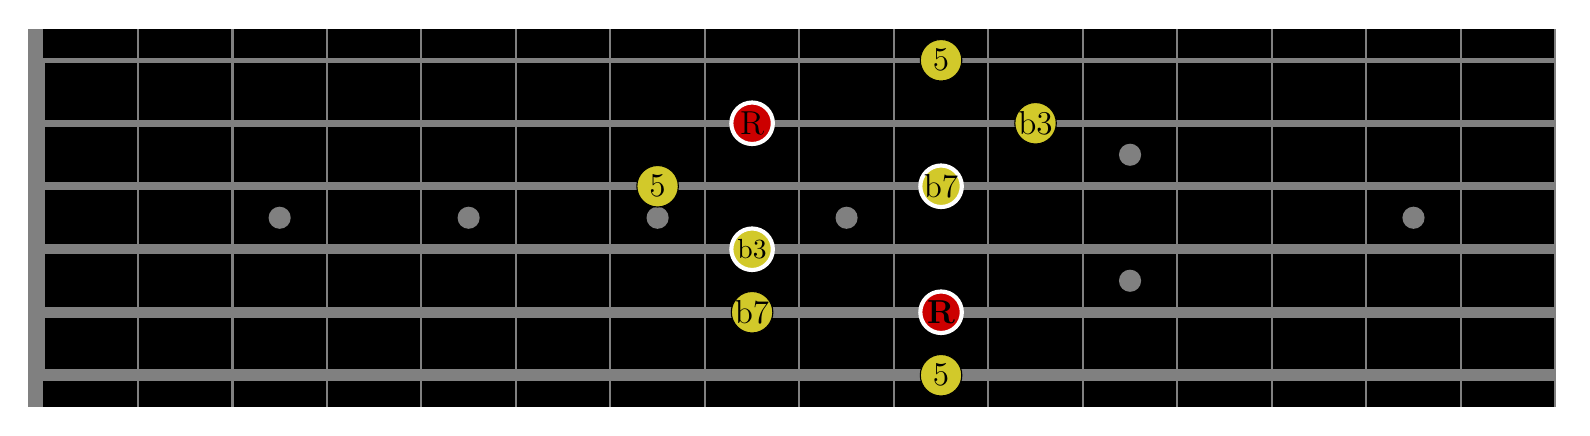
\begin{tikzpicture}[scale=1]
	\def \h{0.8}
	\def \fret{1.2} % 1.6
	\def \L{ 16*\fret }
	\def \dot_size{4pt}
	\def \circ_size{15pt}

	\fill[black, line width=2] (0.0,-0.4) rectangle (16*\fret,4.4);
	\fill[black!50!white, line width=2] (-0.2,-0.4) rectangle (0,4.4);

	% Strings
	\draw[color=black!50!white, line width=2.0]  (-0.1, 5*\h) -- (\L,5*\h); % E
	\draw[color=black!50!white, line width=2.5]  (-0.1, 4*\h) -- (\L,4*\h); % B
	\draw[color=black!50!white, line width=3.0]  (-0.1, 3*\h) -- (\L,3*\h); % G
	\draw[color=black!50!white, line width=3.5]  (-0.1, 2*\h) -- (\L,2*\h); % D
	\draw[color=black!50!white, line width=4.0]  (-0.1, 1*\h) -- (\L,1*\h); % A
	\draw[color=black!50!white, line width=4.5]  (-0.1, 0*\h) -- (\L,0*\h); % E

	% Frets 0
	\draw[color=black!50!white, thick]  (-0.1, 0) -- (-0.1,5*\h);
	\draw[color=black!50!white, thick]  (0, 0)   -- (0,5*\h);

	% Fret 1-15
	\draw[color=black!50!white, thick]  (\fret,   -0.4)   -- (\fret,4.4);
	\draw[color=black!50!white, thick]  (2*\fret, -0.4) -- (2*\fret,4.4);
	\draw[color=black!50!white, thick]  (3*\fret, -0.4) -- (3*\fret,4.4);
	\draw[color=black!50!white, thick]  (4*\fret, -0.4) -- (4*\fret,4.4);
	\draw[color=black!50!white, thick]  (5*\fret, -0.4) -- (5*\fret,4.4);
	\draw[color=black!50!white, thick]  (6*\fret, -0.4) -- (6*\fret,4.4);
	\draw[color=black!50!white, thick]  (7*\fret, -0.4) -- (7*\fret,4.4);
	\draw[color=black!50!white, thick]  (8*\fret, -0.4) -- (8*\fret,4.4);
	\draw[color=black!50!white, thick]  (9*\fret, -0.4) -- (9*\fret,4.4);
	\draw[color=black!50!white, thick]  (10*\fret, -0.4) -- (10*\fret,4.4);
	\draw[color=black!50!white, thick]  (11*\fret, -0.4) -- (11*\fret,4.4);
	\draw[color=black!50!white, thick]  (12*\fret, -0.4) -- (12*\fret,4.4);
	\draw[color=black!50!white, thick]  (13*\fret, -0.4) -- (13*\fret,4.4);
	\draw[color=black!50!white, thick]  (14*\fret, -0.4) -- (14*\fret,4.4);
	\draw[color=black!50!white, thick]  (15*\fret, -0.4) -- (15*\fret,4.4);
	\draw[color=black!50!white, thick]  (16*\fret, -0.4) -- (16*\fret,4.4);
	
	% Dots
	\fill[black!50!white] (2.5*\fret,2.5*\h) circle (\dot_size); % fret 3
	\fill[black!50!white] (4.5*\fret,2.5*\h) circle (\dot_size); % fret 5
	\fill[black!50!white] (6.5*\fret,2.5*\h) circle (\dot_size); % fret 7
	\fill[black!50!white] (8.5*\fret,2.5*\h) circle (\dot_size); % fret 9
	\fill[black!50!white] (11.5*\fret,1.5*\h) circle (\dot_size); % fret 12
	\fill[black!50!white] (11.5*\fret,3.5*\h) circle (\dot_size); % fret 12
	\fill[black!50!white] (14.5*\fret,2.5*\h) circle (\dot_size); % fret 15

	% Arpege (position G-E)
	\node[dot=\circ_size, fill=yellow!80!black,draw] at (9.5*\fret,0*\h) {{\large 5}};
	\node[dot=\circ_size, fill=yellow!80!black,draw] at (7.5*\fret,1*\h) {{\large b7}};
	\node[dot=\circ_size, fill=red!80!black,draw=white, line width=1.5pt] at (9.5*\fret,1*\h) {{\large \textbf{R}}};
	\node[dot=\circ_size, fill=yellow!80!black,draw=white, line width=1.5pt] at (7.5*\fret,2*\h) {{\normalsize b3}};
	\node[dot=\circ_size, fill=yellow!80!black,draw] at (6.5*\fret,3*\h) {{\large 5}};
	\node[dot=\circ_size, fill=yellow!80!black,draw=white, line width=1.5pt] at (9.5*\fret,3*\h) {{\large b7}};
	\node[dot=\circ_size, fill=yellow!80!black,draw] at (10.5*\fret,4*\h) {{\large b3}};
	\node[dot=\circ_size, fill=yellow!80!black,draw] at (9.5*\fret,5*\h) {{\large 5}};
	\node[dot=\circ_size, fill=red!80!black,draw=white, line width=1.5pt] at (7.5*\fret,4*\h) {{\large R}};
%
%	% Annotation
%	\draw[black,anchor=west] (-3cm,2cm) node { {\Huge m7 } };
	
\end{tikzpicture}
%\end{document}




}

	\hspace*{-4.2cm}
	\scalebox{0.52}{

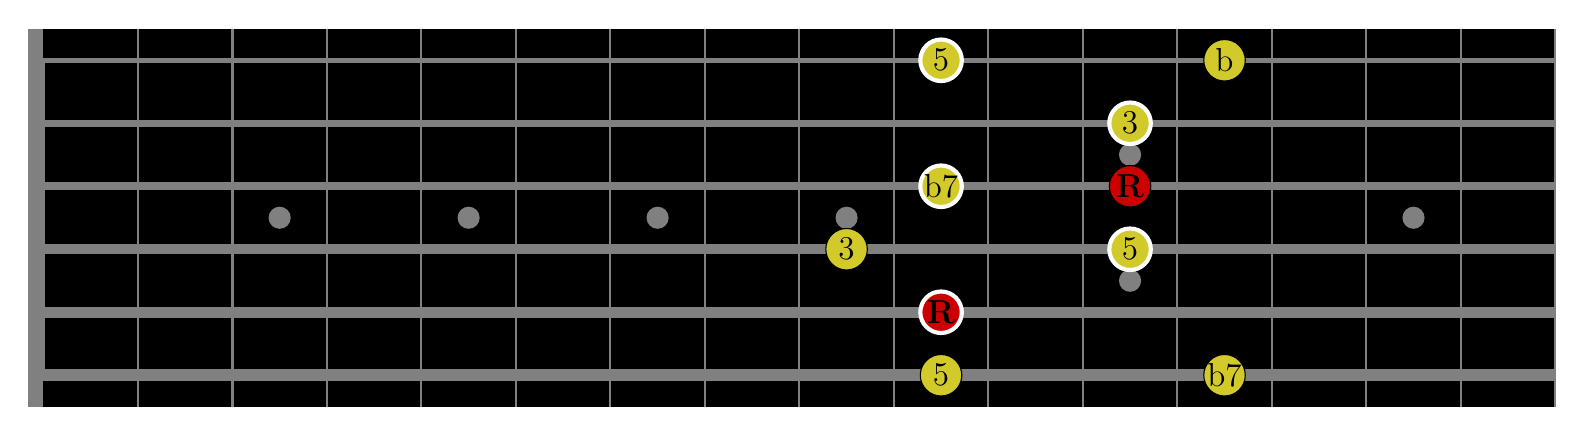
\begin{tikzpicture}[scale=1]
	\def \h{0.8}
	\def \fret{1.2} % 1.6
	\def \L{ 16*\fret }	
	\def \dot_size{4pt}
	\def \circ_size{15pt}
	
	\fill[black, line width=2] (0.0,-0.4) rectangle (16*\fret,4.4);
	\fill[black!50!white, line width=2] (-0.2,-0.4) rectangle (0,4.4);
	
	% Strings
	\draw[color=black!50!white, line width=2.0]  (-0.1, 5*\h) -- (\L,5*\h); % E
	\draw[color=black!50!white, line width=2.5]  (-0.1, 4*\h) -- (\L,4*\h); % B
	\draw[color=black!50!white, line width=3.0]  (-0.1, 3*\h) -- (\L,3*\h); % G
	\draw[color=black!50!white, line width=3.5]  (-0.1, 2*\h) -- (\L,2*\h); % D
	\draw[color=black!50!white, line width=4.0]  (-0.1, 1*\h) -- (\L,1*\h); % A
	\draw[color=black!50!white, line width=4.5]  (-0.1, 0*\h) -- (\L,0*\h); % E
	
	% Frets 0
	\draw[color=black!50!white, thick]  (-0.1, 0) -- (-0.1,5*\h); 
	\draw[color=black!50!white, thick]  (0, 0)   -- (0,5*\h); 
	
	% Fret 1-15
	\draw[color=black!50!white, thick]  (\fret,   -0.4)   -- (\fret,4.4);   
	\draw[color=black!50!white, thick]  (2*\fret, -0.4) -- (2*\fret,4.4); 
	\draw[color=black!50!white, thick]  (3*\fret, -0.4) -- (3*\fret,4.4); 
	\draw[color=black!50!white, thick]  (4*\fret, -0.4) -- (4*\fret,4.4); 
	\draw[color=black!50!white, thick]  (5*\fret, -0.4) -- (5*\fret,4.4); 
	\draw[color=black!50!white, thick]  (6*\fret, -0.4) -- (6*\fret,4.4); 
	\draw[color=black!50!white, thick]  (7*\fret, -0.4) -- (7*\fret,4.4); 
	\draw[color=black!50!white, thick]  (8*\fret, -0.4) -- (8*\fret,4.4); 
	\draw[color=black!50!white, thick]  (9*\fret, -0.4) -- (9*\fret,4.4); 
	\draw[color=black!50!white, thick]  (10*\fret, -0.4) -- (10*\fret,4.4); 
	\draw[color=black!50!white, thick]  (11*\fret, -0.4) -- (11*\fret,4.4); 
	\draw[color=black!50!white, thick]  (12*\fret, -0.4) -- (12*\fret,4.4); 
	\draw[color=black!50!white, thick]  (13*\fret, -0.4) -- (13*\fret,4.4); 
	\draw[color=black!50!white, thick]  (14*\fret, -0.4) -- (14*\fret,4.4); 
	\draw[color=black!50!white, thick]  (15*\fret, -0.4) -- (15*\fret,4.4); 
	\draw[color=black!50!white, thick]  (16*\fret, -0.4) -- (16*\fret,4.4); 
	%\draw[color=black!50!white, thick]  (17*\fret, -0.4) -- (17*\fret,4.4); 
	%\draw[color=black!50!white, thick]  (18*\fret, -0.4) -- (18*\fret,4.4); 
	%\draw[color=black!50!white, thick]  (19*\fret, -0.4) -- (19*\fret,4.4); 
	%\draw[color=black!50!white, thick]  (20*\fret, -0.4) -- (20*\fret,4.4); 
	
	% Dots
	\fill[black!50!white] (2.5*\fret,2.5*\h) circle (\dot_size); % fret 3
	\fill[black!50!white] (4.5*\fret,2.5*\h) circle (\dot_size); % fret 5
	\fill[black!50!white] (6.5*\fret,2.5*\h) circle (\dot_size); % fret 7
	\fill[black!50!white] (8.5*\fret,2.5*\h) circle (\dot_size); % fret 9
	\fill[black!50!white] (11.5*\fret,1.5*\h) circle (\dot_size); % fret 12
	\fill[black!50!white] (11.5*\fret,3.5*\h) circle (\dot_size); % fret 12
	\fill[black!50!white] (14.5*\fret,2.5*\h) circle (\dot_size); % fret 15
	%\fill[black!50!white] (16.5*\fret,2.5*\h) circle (\dot_size); % fret 17
	%\fill[black!50!white] (18.5*\fret,2.5*\h) circle (\dot_size); % fret 19
	
	% String names
%	\draw[black] (-0.5,5*\h) node { {\Large E} };
%	\draw[black] (-0.5,4*\h) node { {\Large B} };
%	\draw[black] (-0.5,3*\h) node { {\Large G} };
%	\draw[black] (-0.5,2*\h) node { {\Large D} };
%	\draw[black] (-0.5,1*\h) node { {\Large A} };
%	\draw[black] (-0.5,0*\h) node { {\Large E} };

	% Notes position
    \node[dot=\circ_size, fill=yellow!80!black,draw] at (12.5*\fret,0*\h) {{\large b7}};
	\node[dot=\circ_size,     fill=yellow!80!black,draw] at (9.5*\fret,0*\h) {{\large 5}};
	\node[dot=\circ_size,     fill=red!80!black,draw=white, line width=1.5pt] at (9.5*\fret,1*\h) {{\large \textbf{R}}};
	\node[dot=\circ_size, fill=yellow!80!black,draw] at (8.5*\fret,2*\h) {{\large 3}};
	\node[dot=\circ_size,     fill=yellow!80!black,draw=white, line width=1.5pt] at (11.5*\fret,2*\h) {{\large 5}};
	\node[dot=\circ_size,     fill=yellow!80!black,draw=white, line width=1.5pt] at (9.5*\fret,3*\h) {{\large b7}};
	\node[dot=\circ_size,     fill=red!80!black,draw] at (11.5*\fret,3*\h) {{\large \textbf{R}}};
	\node[dot=\circ_size,     fill=yellow!80!black,draw=white, line width=1.5pt] at (11.5*\fret,4*\h) {{\large 3}};
	\node[dot=\circ_size,     fill=yellow!80!black,draw=white, line width=1.5pt] at (9.5*\fret,5*\h) {{\large 5}};
	\node[dot=\circ_size,     fill=yellow!80!black,draw] at (12.5*\fret,5*\h) {{\large b}};
%
	% Rectangle
%	\draw [draw=yellow!90!black, line width=1.5] (1.9*\fret,-0.5) rectangle (7.2*\fret,4.5);
%	\draw [draw=yellow!50!red!30!white, line width=1.5] (5.8*\fret,+0.4) rectangle (10.2*\fret,4.5);
%	\draw [draw=yellow!50!red!80!white, line width=1.5] (8.9*\fret,+0.2) rectangle (15.1*\fret,4.6);
	
	% Annotation
%	\draw[black,anchor=west] (-3cm,2cm) node { {\Huge 7 } };
	
\end{tikzpicture}




}
	\hspace*{-0cm}
	\scalebox{0.52}{

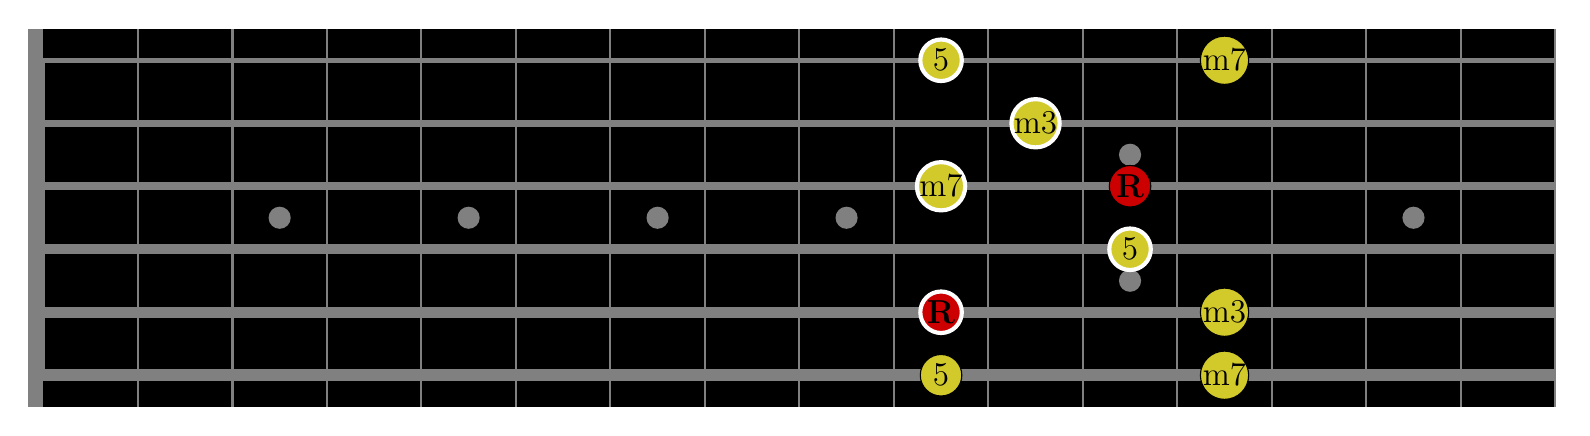
\begin{tikzpicture}[scale=1]
	\def \h{0.8}
	\def \fret{1.2} % 1.6
	\def \L{ 16*\fret }
	\def \dot_size{4pt}
	\def \circ_size{15pt}

	\fill[black, line width=2] (0.0,-0.4) rectangle (16*\fret,4.4);
	\fill[black!50!white, line width=2] (-0.2,-0.4) rectangle (0,4.4);

	% Strings
	\draw[color=black!50!white, line width=2.0]  (-0.1, 5*\h) -- (\L,5*\h); % E
	\draw[color=black!50!white, line width=2.5]  (-0.1, 4*\h) -- (\L,4*\h); % B
	\draw[color=black!50!white, line width=3.0]  (-0.1, 3*\h) -- (\L,3*\h); % G
	\draw[color=black!50!white, line width=3.5]  (-0.1, 2*\h) -- (\L,2*\h); % D
	\draw[color=black!50!white, line width=4.0]  (-0.1, 1*\h) -- (\L,1*\h); % A
	\draw[color=black!50!white, line width=4.5]  (-0.1, 0*\h) -- (\L,0*\h); % E

	% Frets 0
	\draw[color=black!50!white, thick]  (-0.1, 0) -- (-0.1,5*\h);
	\draw[color=black!50!white, thick]  (0, 0)   -- (0,5*\h);

	% Fret 1-15
	\draw[color=black!50!white, thick]  (\fret,   -0.4)   -- (\fret,4.4);
	\draw[color=black!50!white, thick]  (2*\fret, -0.4) -- (2*\fret,4.4);
	\draw[color=black!50!white, thick]  (3*\fret, -0.4) -- (3*\fret,4.4);
	\draw[color=black!50!white, thick]  (4*\fret, -0.4) -- (4*\fret,4.4);
	\draw[color=black!50!white, thick]  (5*\fret, -0.4) -- (5*\fret,4.4);
	\draw[color=black!50!white, thick]  (6*\fret, -0.4) -- (6*\fret,4.4);
	\draw[color=black!50!white, thick]  (7*\fret, -0.4) -- (7*\fret,4.4);
	\draw[color=black!50!white, thick]  (8*\fret, -0.4) -- (8*\fret,4.4);
	\draw[color=black!50!white, thick]  (9*\fret, -0.4) -- (9*\fret,4.4);
	\draw[color=black!50!white, thick]  (10*\fret, -0.4) -- (10*\fret,4.4);
	\draw[color=black!50!white, thick]  (11*\fret, -0.4) -- (11*\fret,4.4);
	\draw[color=black!50!white, thick]  (12*\fret, -0.4) -- (12*\fret,4.4);
	\draw[color=black!50!white, thick]  (13*\fret, -0.4) -- (13*\fret,4.4);
	\draw[color=black!50!white, thick]  (14*\fret, -0.4) -- (14*\fret,4.4);
	\draw[color=black!50!white, thick]  (15*\fret, -0.4) -- (15*\fret,4.4);
	\draw[color=black!50!white, thick]  (16*\fret, -0.4) -- (16*\fret,4.4);
	
	% Dots
	\fill[black!50!white] (2.5*\fret,2.5*\h) circle (\dot_size); % fret 3
	\fill[black!50!white] (4.5*\fret,2.5*\h) circle (\dot_size); % fret 5
	\fill[black!50!white] (6.5*\fret,2.5*\h) circle (\dot_size); % fret 7
	\fill[black!50!white] (8.5*\fret,2.5*\h) circle (\dot_size); % fret 9
	\fill[black!50!white] (11.5*\fret,1.5*\h) circle (\dot_size); % fret 12
	\fill[black!50!white] (11.5*\fret,3.5*\h) circle (\dot_size); % fret 12
	\fill[black!50!white] (14.5*\fret,2.5*\h) circle (\dot_size); % fret 15

	% Arpege (position G-E)
	\node[dot=\circ_size, fill=yellow!80!black,draw] at (9.5*\fret,0*\h) {{\large 5}};
	\node[dot=\circ_size, fill=yellow!80!black,draw] at (12.5*\fret,0*\h) {{\large m7}};
	\node[dot=\circ_size, fill=yellow!80!black,draw] at (12.5*\fret,1*\h) {{\large m3}};
	\node[dot=\circ_size, fill=red!80!black,draw=white, line width=1.5pt] at (9.5*\fret,1*\h) {{\large \textbf{R}}};
	\node[dot=\circ_size, fill=yellow!80!black,draw=white, line width=1.5pt] at (11.5*\fret,2*\h) {{\large 5}};
	\node[dot=\circ_size, fill=red!80!black,draw] at (11.5*\fret,3*\h) {{\large \textbf{R}}};
	\node[dot=\circ_size, fill=yellow!80!black,draw=white, line width=1.5pt] at (9.5*\fret,3*\h) {{\large m7}};
	\node[dot=\circ_size, fill=yellow!80!black,draw=white, line width=1.5pt] at (10.5*\fret,4*\h) {{\large m3}};
	\node[dot=\circ_size, fill=yellow!80!black,draw=white, line width=1.5pt] at (9.5*\fret,5*\h) {{\large 5}};
	\node[dot=\circ_size, fill=yellow!80!black,draw] at (12.5*\fret,5*\h) {{\large m7}};
%
%	% Annotation
%	\draw[black,anchor=west] (-3cm,2cm) node { {\Huge m7 } };
	
\end{tikzpicture}
%\end{document}




}

	\hspace*{-4.2cm}
	\scalebox{0.52}{

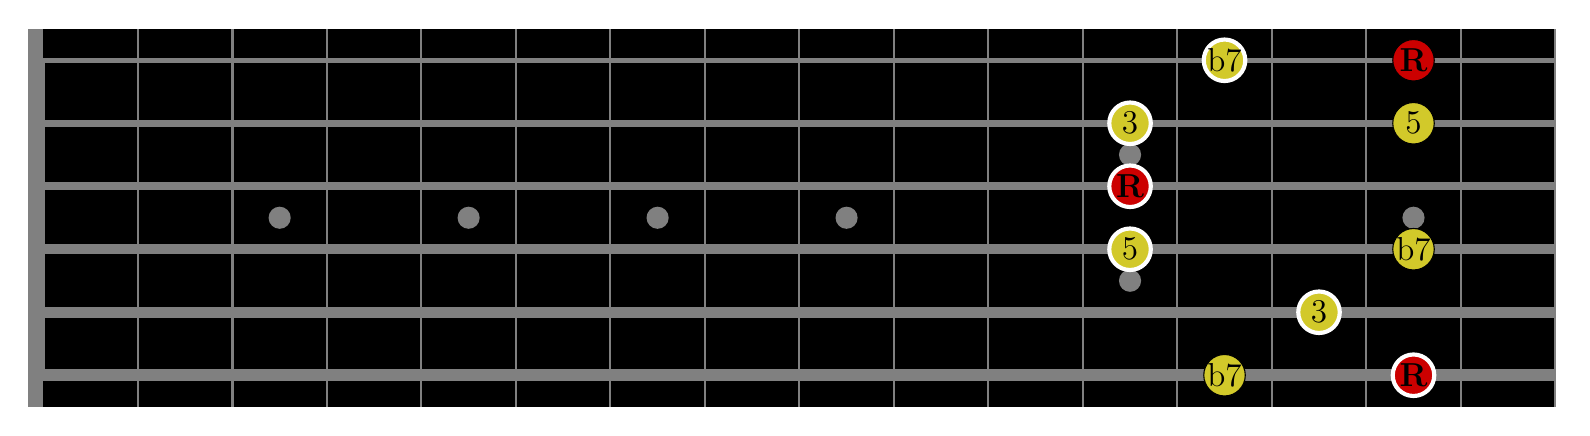
\begin{tikzpicture}[scale=1]
	\def \h{0.8}
	\def \fret{1.2} % 1.6
	\def \L{ 16*\fret }	
	\def \dot_size{4pt}
	\def \circ_size{15pt}
	
	\fill[black, line width=2] (0.0,-0.4) rectangle (16*\fret,4.4);
	\fill[black!50!white, line width=2] (-0.2,-0.4) rectangle (0,4.4);
	
	% Strings
	\draw[color=black!50!white, line width=2.0]  (-0.1, 5*\h) -- (\L,5*\h); % E
	\draw[color=black!50!white, line width=2.5]  (-0.1, 4*\h) -- (\L,4*\h); % B
	\draw[color=black!50!white, line width=3.0]  (-0.1, 3*\h) -- (\L,3*\h); % G
	\draw[color=black!50!white, line width=3.5]  (-0.1, 2*\h) -- (\L,2*\h); % D
	\draw[color=black!50!white, line width=4.0]  (-0.1, 1*\h) -- (\L,1*\h); % A
	\draw[color=black!50!white, line width=4.5]  (-0.1, 0*\h) -- (\L,0*\h); % E
	
	% Frets 0
	\draw[color=black!50!white, thick]  (-0.1, 0) -- (-0.1,5*\h); 
	\draw[color=black!50!white, thick]  (0, 0)   -- (0,5*\h); 
	
	% Fret 1-15
	\draw[color=black!50!white, thick]  (\fret,   -0.4)   -- (\fret,4.4);   
	\draw[color=black!50!white, thick]  (2*\fret, -0.4) -- (2*\fret,4.4); 
	\draw[color=black!50!white, thick]  (3*\fret, -0.4) -- (3*\fret,4.4); 
	\draw[color=black!50!white, thick]  (4*\fret, -0.4) -- (4*\fret,4.4); 
	\draw[color=black!50!white, thick]  (5*\fret, -0.4) -- (5*\fret,4.4); 
	\draw[color=black!50!white, thick]  (6*\fret, -0.4) -- (6*\fret,4.4); 
	\draw[color=black!50!white, thick]  (7*\fret, -0.4) -- (7*\fret,4.4); 
	\draw[color=black!50!white, thick]  (8*\fret, -0.4) -- (8*\fret,4.4); 
	\draw[color=black!50!white, thick]  (9*\fret, -0.4) -- (9*\fret,4.4); 
	\draw[color=black!50!white, thick]  (10*\fret, -0.4) -- (10*\fret,4.4); 
	\draw[color=black!50!white, thick]  (11*\fret, -0.4) -- (11*\fret,4.4); 
	\draw[color=black!50!white, thick]  (12*\fret, -0.4) -- (12*\fret,4.4); 
	\draw[color=black!50!white, thick]  (13*\fret, -0.4) -- (13*\fret,4.4); 
	\draw[color=black!50!white, thick]  (14*\fret, -0.4) -- (14*\fret,4.4); 
	\draw[color=black!50!white, thick]  (15*\fret, -0.4) -- (15*\fret,4.4); 
	\draw[color=black!50!white, thick]  (16*\fret, -0.4) -- (16*\fret,4.4); 
	%\draw[color=black!50!white, thick]  (17*\fret, -0.4) -- (17*\fret,4.4); 
	%\draw[color=black!50!white, thick]  (18*\fret, -0.4) -- (18*\fret,4.4); 
	%\draw[color=black!50!white, thick]  (19*\fret, -0.4) -- (19*\fret,4.4); 
	%\draw[color=black!50!white, thick]  (20*\fret, -0.4) -- (20*\fret,4.4); 
	
	% Dots
	\fill[black!50!white] (2.5*\fret,2.5*\h) circle (\dot_size); % fret 3
	\fill[black!50!white] (4.5*\fret,2.5*\h) circle (\dot_size); % fret 5
	\fill[black!50!white] (6.5*\fret,2.5*\h) circle (\dot_size); % fret 7
	\fill[black!50!white] (8.5*\fret,2.5*\h) circle (\dot_size); % fret 9
	\fill[black!50!white] (11.5*\fret,1.5*\h) circle (\dot_size); % fret 12
	\fill[black!50!white] (11.5*\fret,3.5*\h) circle (\dot_size); % fret 12
	\fill[black!50!white] (14.5*\fret,2.5*\h) circle (\dot_size); % fret 15
	%\fill[black!50!white] (16.5*\fret,2.5*\h) circle (\dot_size); % fret 17
	%\fill[black!50!white] (18.5*\fret,2.5*\h) circle (\dot_size); % fret 19
	
	% String names
%	\draw[black] (-0.5,5*\h) node { {\Large E} };
%	\draw[black] (-0.5,4*\h) node { {\Large B} };
%	\draw[black] (-0.5,3*\h) node { {\Large G} };
%	\draw[black] (-0.5,2*\h) node { {\Large D} };
%	\draw[black] (-0.5,1*\h) node { {\Large A} };
%	\draw[black] (-0.5,0*\h) node { {\Large E} };

	% Notes position
    \node[dot=\circ_size, fill=yellow!80!black,draw] at (12.5*\fret,0*\h) {{\large b7}};
	\node[dot=\circ_size, fill=red!80!black,draw=white, line width=1.5pt] at (14.5*\fret,0*\h) {{\large \textbf{R}}};
	\node[dot=\circ_size, fill=yellow!80!black,draw=white, line width=1.5pt] at (13.5*\fret,1*\h) {{\large 3}};
	\node[dot=\circ_size, fill=yellow!80!black,draw] at (14.5*\fret,2*\h) {{\large b7}};
	\node[dot=\circ_size, fill=yellow!80!black,draw=white, line width=1.5pt] at (11.5*\fret,2*\h) {{\large 5}};
	\node[dot=\circ_size, fill=red!80!black,draw=white, line width=1.5pt] at (11.5*\fret,3*\h) {{\large \textbf{R}}};
	\node[dot=\circ_size, fill=yellow!80!black,draw=white, line width=1.5pt] at (11.5*\fret,4*\h) {{\large 3}};
	\node[dot=\circ_size, fill=yellow!80!black,draw] at (14.5*\fret,4*\h) {{\large 5}};
	\node[dot=\circ_size, fill=yellow!80!black,draw=white, line width=1.5pt] at (12.5*\fret,5*\h) {{\large b7}};
	\node[dot=\circ_size, fill=red!80!black,draw] at (14.5*\fret,5*\h) {{\large \textbf{R}}};
%
	% Rectangle
%	\draw [draw=yellow!90!black, line width=1.5] (1.9*\fret,-0.5) rectangle (7.2*\fret,4.5);
%	\draw [draw=yellow!50!red!30!white, line width=1.5] (5.8*\fret,+0.4) rectangle (10.2*\fret,4.5);
%	\draw [draw=yellow!50!red!80!white, line width=1.5] (8.9*\fret,+0.2) rectangle (15.1*\fret,4.6);
	
	% Annotation
%	\draw[black,anchor=west] (-3cm,2cm) node { {\Huge 7 } };
	
\end{tikzpicture}




}
	\hspace*{-0cm}
	\scalebox{0.52}{

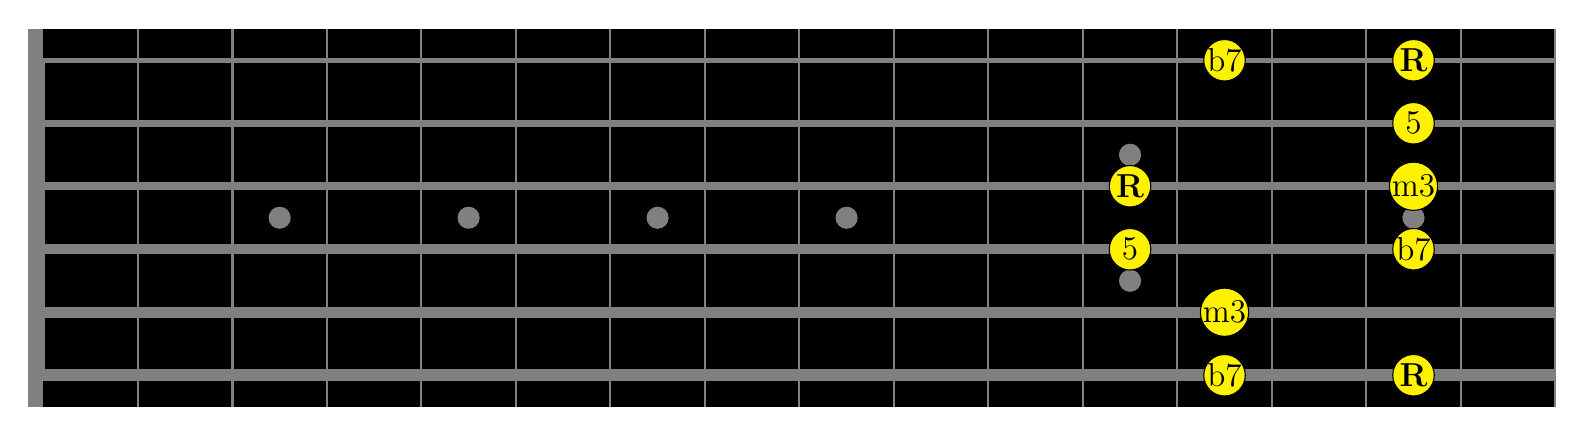
\begin{tikzpicture}[scale=1]
	\def \h{0.8}
	\def \fret{1.2} % 1.6
	\def \L{ 16*\fret }
	\def \dot_size{4pt}
	\def \circ_size{15pt}

	\fill[black, line width=2] (0.0,-0.4) rectangle (16*\fret,4.4);
	\fill[black!50!white, line width=2] (-0.2,-0.4) rectangle (0,4.4);

	% Strings
	\draw[color=black!50!white, line width=2.0]  (-0.1, 5*\h) -- (\L,5*\h); % E
	\draw[color=black!50!white, line width=2.5]  (-0.1, 4*\h) -- (\L,4*\h); % B
	\draw[color=black!50!white, line width=3.0]  (-0.1, 3*\h) -- (\L,3*\h); % G
	\draw[color=black!50!white, line width=3.5]  (-0.1, 2*\h) -- (\L,2*\h); % D
	\draw[color=black!50!white, line width=4.0]  (-0.1, 1*\h) -- (\L,1*\h); % A
	\draw[color=black!50!white, line width=4.5]  (-0.1, 0*\h) -- (\L,0*\h); % E

	% Frets 0
	\draw[color=black!50!white, thick]  (-0.1, 0) -- (-0.1,5*\h);
	\draw[color=black!50!white, thick]  (0, 0)   -- (0,5*\h);

	% Fret 1-15
	\draw[color=black!50!white, thick]  (\fret,   -0.4)   -- (\fret,4.4);
	\draw[color=black!50!white, thick]  (2*\fret, -0.4) -- (2*\fret,4.4);
	\draw[color=black!50!white, thick]  (3*\fret, -0.4) -- (3*\fret,4.4);
	\draw[color=black!50!white, thick]  (4*\fret, -0.4) -- (4*\fret,4.4);
	\draw[color=black!50!white, thick]  (5*\fret, -0.4) -- (5*\fret,4.4);
	\draw[color=black!50!white, thick]  (6*\fret, -0.4) -- (6*\fret,4.4);
	\draw[color=black!50!white, thick]  (7*\fret, -0.4) -- (7*\fret,4.4);
	\draw[color=black!50!white, thick]  (8*\fret, -0.4) -- (8*\fret,4.4);
	\draw[color=black!50!white, thick]  (9*\fret, -0.4) -- (9*\fret,4.4);
	\draw[color=black!50!white, thick]  (10*\fret, -0.4) -- (10*\fret,4.4);
	\draw[color=black!50!white, thick]  (11*\fret, -0.4) -- (11*\fret,4.4);
	\draw[color=black!50!white, thick]  (12*\fret, -0.4) -- (12*\fret,4.4);
	\draw[color=black!50!white, thick]  (13*\fret, -0.4) -- (13*\fret,4.4);
	\draw[color=black!50!white, thick]  (14*\fret, -0.4) -- (14*\fret,4.4);
	\draw[color=black!50!white, thick]  (15*\fret, -0.4) -- (15*\fret,4.4);
	\draw[color=black!50!white, thick]  (16*\fret, -0.4) -- (16*\fret,4.4);
	
	% Dots
	\fill[black!50!white] (2.5*\fret,2.5*\h) circle (\dot_size); % fret 3
	\fill[black!50!white] (4.5*\fret,2.5*\h) circle (\dot_size); % fret 5
	\fill[black!50!white] (6.5*\fret,2.5*\h) circle (\dot_size); % fret 7
	\fill[black!50!white] (8.5*\fret,2.5*\h) circle (\dot_size); % fret 9
	\fill[black!50!white] (11.5*\fret,1.5*\h) circle (\dot_size); % fret 12
	\fill[black!50!white] (11.5*\fret,3.5*\h) circle (\dot_size); % fret 12
	\fill[black!50!white] (14.5*\fret,2.5*\h) circle (\dot_size); % fret 15

	% Arpege (position G-E)
	\node[dot=\circ_size, fill=yellow,draw] at (14.5*\fret,0*\h) {{\large \textbf{R}}};
	\node[dot=\circ_size, fill=yellow,draw] at (12.5*\fret,0*\h) {{\large b7}};
	\node[dot=\circ_size, fill=yellow,draw] at (12.5*\fret,1*\h) {{\large m3}};
	\node[dot=\circ_size, fill=yellow,draw] at (11.5*\fret,2*\h) {{\large 5}};
	\node[dot=\circ_size, fill=yellow,draw] at (14.5*\fret,2*\h) {{\large b7}};
	\node[dot=\circ_size, fill=yellow,draw] at (11.5*\fret,3*\h) {{\large \textbf{R}}};
	\node[dot=\circ_size, fill=yellow,draw] at (14.5*\fret,3*\h) {{\large m3}};
	\node[dot=\circ_size, fill=yellow,draw] at (14.5*\fret,4*\h) {{\large 5}};
	\node[dot=\circ_size, fill=yellow,draw] at (12.5*\fret,5*\h) {{\large b7}};
	\node[dot=\circ_size, fill=yellow,draw] at (14.5*\fret,5*\h) {{\large \textbf{R}}};
%
%	% Annotation
%	\draw[black,anchor=west] (-3cm,2cm) node { {\Huge m7 } };
	
\end{tikzpicture}
%\end{document}




}

	\caption{(left) dom7 arpeggio. (right) m7 arpeggio}
	\label{fig:arpeggio}
\end{table}


% Figure
\begin{table}[!h]
	\hspace*{-4.2cm}
	\scalebox{0.52}{%\documentclass{standalone}
%\usepackage{pgfplots} % Include package for TikZ and PGF plot
%\usepackage{anyfontsize} % enable to change the font size manually
%\usepackage{makecell}%
%\usetikzlibrary{shapes.geometric}
%\tikzset{
%dot/.style = {circle, fill, minimum size=#1,
%              inner sep=0pt, outer sep=0pt},
%dot/.default = 6pt % size of the circle diameter
%}
% \renewcommand{\familydefault}{\sfdefault}

%\begin{document}
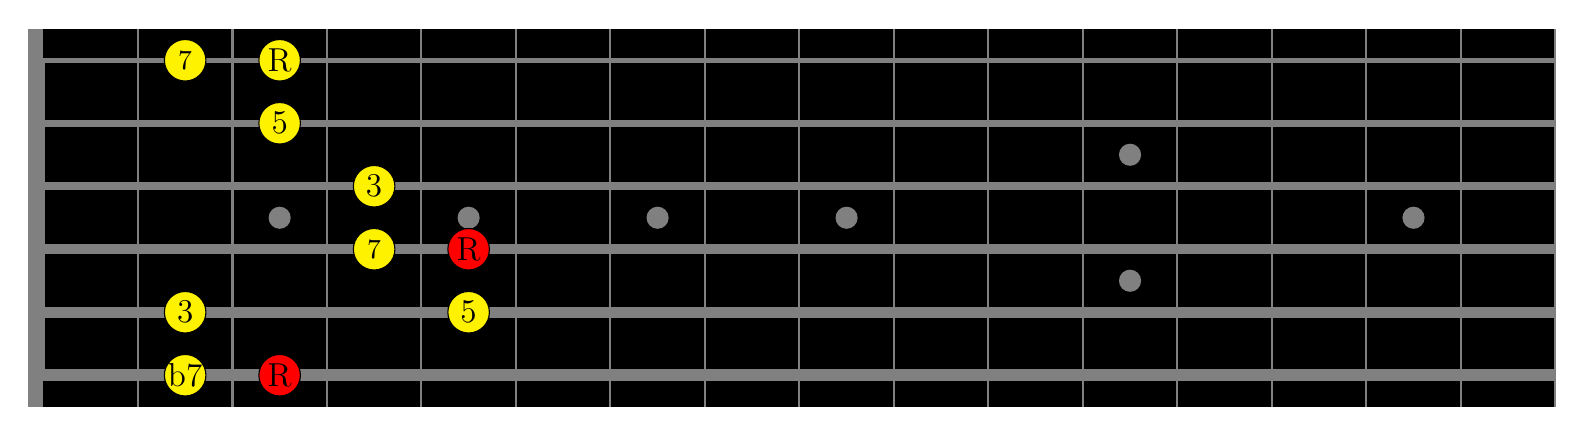
\begin{tikzpicture}[scale=1]
	\def \h{0.8}
	\def \fret{1.2} % 1.6
	\def \L{ 16*\fret }	
	\def \dot_size{4pt}
	\def \circ_size{15pt}
	
	\fill[black, line width=2] (0.0,-0.4) rectangle (16*\fret,4.4);
	\fill[black!50!white, line width=2] (-0.2,-0.4) rectangle (0,4.4);
	
	% Strings
	\draw[color=black!50!white, line width=2.0]  (-0.1, 5*\h) -- (\L,5*\h); % E
	\draw[color=black!50!white, line width=2.5]  (-0.1, 4*\h) -- (\L,4*\h); % B
	\draw[color=black!50!white, line width=3.0]  (-0.1, 3*\h) -- (\L,3*\h); % G
	\draw[color=black!50!white, line width=3.5]  (-0.1, 2*\h) -- (\L,2*\h); % D
	\draw[color=black!50!white, line width=4.0]  (-0.1, 1*\h) -- (\L,1*\h); % A
	\draw[color=black!50!white, line width=4.5]  (-0.1, 0*\h) -- (\L,0*\h); % E
	
	% Frets 0
	\draw[color=black!50!white, thick]  (-0.1, 0) -- (-0.1,5*\h); 
	\draw[color=black!50!white, thick]  (0, 0)   -- (0,5*\h); 
	
	% Fret 1-15
	\draw[color=black!50!white, thick]  (\fret,   -0.4)   -- (\fret,4.4);   
	\draw[color=black!50!white, thick]  (2*\fret, -0.4) -- (2*\fret,4.4); 
	\draw[color=black!50!white, thick]  (3*\fret, -0.4) -- (3*\fret,4.4); 
	\draw[color=black!50!white, thick]  (4*\fret, -0.4) -- (4*\fret,4.4); 
	\draw[color=black!50!white, thick]  (5*\fret, -0.4) -- (5*\fret,4.4); 
	\draw[color=black!50!white, thick]  (6*\fret, -0.4) -- (6*\fret,4.4); 
	\draw[color=black!50!white, thick]  (7*\fret, -0.4) -- (7*\fret,4.4); 
	\draw[color=black!50!white, thick]  (8*\fret, -0.4) -- (8*\fret,4.4); 
	\draw[color=black!50!white, thick]  (9*\fret, -0.4) -- (9*\fret,4.4); 
	\draw[color=black!50!white, thick]  (10*\fret, -0.4) -- (10*\fret,4.4); 
	\draw[color=black!50!white, thick]  (11*\fret, -0.4) -- (11*\fret,4.4); 
	\draw[color=black!50!white, thick]  (12*\fret, -0.4) -- (12*\fret,4.4); 
	\draw[color=black!50!white, thick]  (13*\fret, -0.4) -- (13*\fret,4.4); 
	\draw[color=black!50!white, thick]  (14*\fret, -0.4) -- (14*\fret,4.4); 
	\draw[color=black!50!white, thick]  (15*\fret, -0.4) -- (15*\fret,4.4); 
	\draw[color=black!50!white, thick]  (16*\fret, -0.4) -- (16*\fret,4.4); 
	%\draw[color=black!50!white, thick]  (17*\fret, -0.4) -- (17*\fret,4.4); 
	%\draw[color=black!50!white, thick]  (18*\fret, -0.4) -- (18*\fret,4.4); 
	%\draw[color=black!50!white, thick]  (19*\fret, -0.4) -- (19*\fret,4.4); 
	%\draw[color=black!50!white, thick]  (20*\fret, -0.4) -- (20*\fret,4.4); 
	
	% Dots
	\fill[black!50!white] (2.5*\fret,2.5*\h) circle (\dot_size); % fret 3
	\fill[black!50!white] (4.5*\fret,2.5*\h) circle (\dot_size); % fret 5
	\fill[black!50!white] (6.5*\fret,2.5*\h) circle (\dot_size); % fret 7
	\fill[black!50!white] (8.5*\fret,2.5*\h) circle (\dot_size); % fret 9
	\fill[black!50!white] (11.5*\fret,1.5*\h) circle (\dot_size); % fret 12
	\fill[black!50!white] (11.5*\fret,3.5*\h) circle (\dot_size); % fret 12
	\fill[black!50!white] (14.5*\fret,2.5*\h) circle (\dot_size); % fret 15
	%\fill[black!50!white] (16.5*\fret,2.5*\h) circle (\dot_size); % fret 17
	%\fill[black!50!white] (18.5*\fret,2.5*\h) circle (\dot_size); % fret 19

	
	% Arpege (position E)
	\node[dot=\circ_size, fill=yellow,draw] at (1.5*\fret,0) {{\large b7}};
	\node[dot=\circ_size, fill=red,draw] at (2.5*\fret,0) {{\large R}};
	\node[dot=\circ_size, fill=yellow,draw] at (1.5*\fret,1*\h) {{\large 3}};
	%\node[dot=\circ_size, fill=yellow,draw] at (1.5*\fret,1*\h) {{\large 3}};
	\node[dot=\circ_size, fill=yellow,draw] at (4.5*\fret,1*\h) {{\large 5}};
	\node[dot=\circ_size, fill=yellow,draw] at (3.5*\fret,2*\h) {{\normalsize 7}};
	\node[dot=\circ_size, fill=red,draw] at (4.5*\fret,2*\h) {{\large R}};
	\node[dot=\circ_size, fill=yellow,draw] at (3.5*\fret,3*\h) {{\large 3}};
	\node[dot=\circ_size, fill=yellow,draw] at (2.5*\fret,4*\h) {{\large 5}};
	\node[dot=\circ_size, fill=yellow,draw] at (1.5*\fret,5*\h) {{\normalsize 7}};
	\node[dot=\circ_size, fill=yellow,draw] at (2.5*\fret,5*\h) {{\large R}};
	
%	% Arpege (position D-C)
%	\node[dot=\circ_size, fill=white,draw] at (8.5*\fret,1*\h) {{\normalsize 7}};
%	\node[dot=\circ_size, fill=yellow!50!red!65!white,draw] at (9.5*\fret,1*\h) {{\large R}};
%	\node[dot=\circ_size, fill=yellow!50!red!30!white,draw] at (8.5*\fret,2*\h) {{\large 3}};
%	\node[dot=\circ_size, fill=yellow!50!red!30!white,draw] at (6.5*\fret,3*\h) {{\large 5}};
%	\node[dot=\circ_size, fill=white,draw] at (6.5*\fret,4*\h) {{\normalsize M7}};
%	\node[dot=\circ_size, fill=yellow!50!red!30!white,draw] at (7.5*\fret,4*\h) {{\large R}};
%	\node[dot=\circ_size, fill=yellow!100!red!50!white,draw] at (6.5*\fret,5*\h) {{\large 3}};
%	\node[dot=\circ_size, fill=yellow!50!red!65!white,draw] at (9.5*\fret,5*\h) {{\large 5}};
	
	% Arpege (position A)
%	\node[dot=\circ_size, fill=yellow!50!red!80!white,draw] at (13.5*\fret,1*\h) {{\large 3}};
%	\node[dot=\circ_size, fill=yellow!50!red!80!white,draw] at (11.5*\fret,2*\h) {{\large 5}};
%	\node[dot=\circ_size, fill=white,draw] at (10.5*\fret,3*\h) {{\normalsize M7}};
%	\node[dot=\circ_size, fill=yellow!50!red!80!white,draw] at (11.5*\fret,3*\h) {{\large R}};
%	\node[dot=\circ_size, fill=yellow!50!red!80!white,draw] at (11.5*\fret,4*\h) {{\large 3}};
%	\node[dot=\circ_size, fill=white,draw] at (13.5*\fret,5*\h) {{\normalsize M7}};
%	\node[dot=\circ_size, fill=yellow!50!red!80!white,draw] at (14.5*\fret,5*\h) {{\large R}};

%	% Annotation
%	\draw[black,anchor=west] (-3cm,2cm) node { {\Huge $\Delta$7 } };
	
\end{tikzpicture}
%\end{document}




}
	\hspace*{-0cm}
	\scalebox{0.52}{%\documentclass{standalone}
%\usepackage{pgfplots} % Include package for TikZ and PGF plot
%\usepackage{anyfontsize} % enable to change the font size manually
%\usepackage{makecell}%
%\usetikzlibrary{shapes.geometric}
%\tikzset{
%dot/.style = {circle, fill, minimum size=#1,
%              inner sep=0pt, outer sep=0pt},
%dot/.default = 6pt % size of the circle diameter
%}
% \renewcommand{\familydefault}{\sfdefault}

%\begin{document}
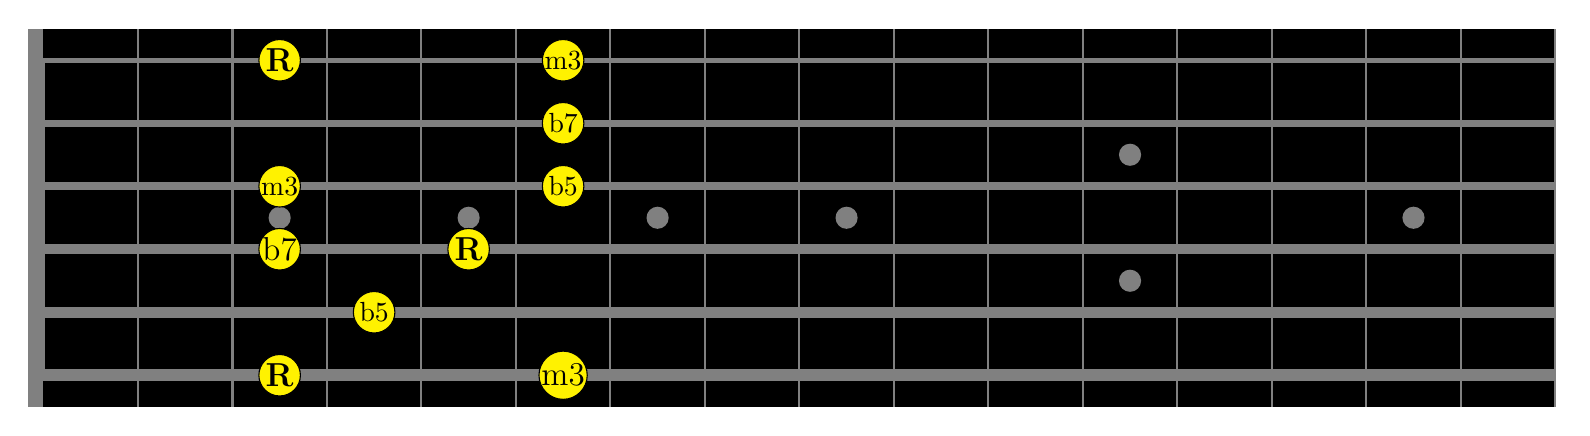
\begin{tikzpicture}[scale=1]
	\def \h{0.8}
	\def \fret{1.2} % 1.6
	\def \L{ 16*\fret }	
	\def \dot_size{4pt}
	\def \circ_size{15pt}
	
	\fill[black, line width=2] (0.0,-0.4) rectangle (16*\fret,4.4);
	\fill[black!50!white, line width=2] (-0.2,-0.4) rectangle (0,4.4);
	
	% Strings
	\draw[color=black!50!white, line width=2.0]  (-0.1, 5*\h) -- (\L,5*\h); % E
	\draw[color=black!50!white, line width=2.5]  (-0.1, 4*\h) -- (\L,4*\h); % B
	\draw[color=black!50!white, line width=3.0]  (-0.1, 3*\h) -- (\L,3*\h); % G
	\draw[color=black!50!white, line width=3.5]  (-0.1, 2*\h) -- (\L,2*\h); % D
	\draw[color=black!50!white, line width=4.0]  (-0.1, 1*\h) -- (\L,1*\h); % A
	\draw[color=black!50!white, line width=4.5]  (-0.1, 0*\h) -- (\L,0*\h); % E
	
	% Frets 0
	\draw[color=black!50!white, thick]  (-0.1, 0) -- (-0.1,5*\h); 
	\draw[color=black!50!white, thick]  (0, 0)   -- (0,5*\h); 
	
	% Fret 1-15
	\draw[color=black!50!white, thick]  (\fret,   -0.4)   -- (\fret,4.4);   
	\draw[color=black!50!white, thick]  (2*\fret, -0.4) -- (2*\fret,4.4); 
	\draw[color=black!50!white, thick]  (3*\fret, -0.4) -- (3*\fret,4.4); 
	\draw[color=black!50!white, thick]  (4*\fret, -0.4) -- (4*\fret,4.4); 
	\draw[color=black!50!white, thick]  (5*\fret, -0.4) -- (5*\fret,4.4); 
	\draw[color=black!50!white, thick]  (6*\fret, -0.4) -- (6*\fret,4.4); 
	\draw[color=black!50!white, thick]  (7*\fret, -0.4) -- (7*\fret,4.4); 
	\draw[color=black!50!white, thick]  (8*\fret, -0.4) -- (8*\fret,4.4); 
	\draw[color=black!50!white, thick]  (9*\fret, -0.4) -- (9*\fret,4.4); 
	\draw[color=black!50!white, thick]  (10*\fret, -0.4) -- (10*\fret,4.4); 
	\draw[color=black!50!white, thick]  (11*\fret, -0.4) -- (11*\fret,4.4); 
	\draw[color=black!50!white, thick]  (12*\fret, -0.4) -- (12*\fret,4.4); 
	\draw[color=black!50!white, thick]  (13*\fret, -0.4) -- (13*\fret,4.4); 
	\draw[color=black!50!white, thick]  (14*\fret, -0.4) -- (14*\fret,4.4); 
	\draw[color=black!50!white, thick]  (15*\fret, -0.4) -- (15*\fret,4.4); 
	\draw[color=black!50!white, thick]  (16*\fret, -0.4) -- (16*\fret,4.4); 
	%\draw[color=black!50!white, thick]  (17*\fret, -0.4) -- (17*\fret,4.4); 
	%\draw[color=black!50!white, thick]  (18*\fret, -0.4) -- (18*\fret,4.4); 
	%\draw[color=black!50!white, thick]  (19*\fret, -0.4) -- (19*\fret,4.4); 
	%\draw[color=black!50!white, thick]  (20*\fret, -0.4) -- (20*\fret,4.4); 
	
	% Dots
	\fill[black!50!white] (2.5*\fret,2.5*\h) circle (\dot_size); % fret 3
	\fill[black!50!white] (4.5*\fret,2.5*\h) circle (\dot_size); % fret 5
	\fill[black!50!white] (6.5*\fret,2.5*\h) circle (\dot_size); % fret 7
	\fill[black!50!white] (8.5*\fret,2.5*\h) circle (\dot_size); % fret 9
	\fill[black!50!white] (11.5*\fret,1.5*\h) circle (\dot_size); % fret 12
	\fill[black!50!white] (11.5*\fret,3.5*\h) circle (\dot_size); % fret 12
	\fill[black!50!white] (14.5*\fret,2.5*\h) circle (\dot_size); % fret 15
	%\fill[black!50!white] (16.5*\fret,2.5*\h) circle (\dot_size); % fret 17
	%\fill[black!50!white] (18.5*\fret,2.5*\h) circle (\dot_size); % fret 19

	
	% Arpege (position A)
	\node[dot=\circ_size, fill=yellow,draw] at (5.5*\fret,0) {{\large m3}};
	\node[dot=\circ_size, fill=yellow,draw] at (2.5*\fret,0) {{\large \textbf{R}}};
	\node[dot=\circ_size, fill=yellow,draw] at (3.5*\fret,1*\h) {{\normalsize b5}};
	\node[dot=\circ_size, fill=yellow,draw] at (2.5*\fret,2*\h) {{\large b7}};
	\node[dot=\circ_size, fill=yellow,draw] at (4.5*\fret,2*\h) {{\large \textbf{R}}};
	\node[dot=\circ_size, fill=yellow,draw] at (2.5*\fret,3*\h) {{\normalsize m3}};
	\node[dot=\circ_size, fill=yellow,draw] at (5.5*\fret,3*\h) {{\normalsize b5}};
	\node[dot=\circ_size, fill=yellow,draw] at (5.5*\fret,4*\h) {{\normalsize b7}};
	\node[dot=\circ_size, fill=yellow,draw] at (5.5*\fret,5*\h) {{\normalsize m3}};
	\node[dot=\circ_size, fill=yellow,draw] at (2.5*\fret,5*\h) {{\large \textbf{R}}};
	
%	% Arpege (position G-E)
%	\node[dot=\circ_size, fill=yellow!50!red!30!white,draw] at (5.5*\fret,0*\h) {{\normalsize m3}};
%	\node[dot=\circ_size, fill=yellow!50!red!30!white,draw] at (8.5*\fret,0*\h) {{\normalsize b5}};
%	\node[dot=\circ_size, fill=white,draw] at (7.5*\fret,1*\h) {{\large 7}};
%	\node[dot=\circ_size, fill=yellow!50!red!30!white,draw] at (9.5*\fret,1*\h) {{\large R}};
%	\node[dot=\circ_size, fill=yellow!50!red!30!white,draw] at (7.5*\fret,2*\h) {{\normalsize 3m}};
%	\node[dot=\circ_size, fill=yellow!50!red!30!white,draw] at (5.5*\fret,3*\h) {{\normalsize b5}};
%	\node[dot=\circ_size, fill=white,draw] at (5.5*\fret,4*\h) {{\large 7}};
%	\node[dot=\circ_size, fill=yellow!50!red!30!white,draw] at (7.5*\fret,4*\h) {{\large R}};
%	\node[dot=\circ_size, fill=yellow!50!red!30!white,draw] at (5.5*\fret,5*\h) {{\normalsize m3}};
%	\node[dot=\circ_size, fill=yellow!50!red!30!white,draw] at (8.5*\fret,5*\h) {{\normalsize b5}};
%
%	% Arpege (position D-C)
%	\node[dot=\circ_size, fill=yellow!50!red!80!white,draw] at (12.5*\fret,1*\h) {{\normalsize m3}};
%	\node[dot=\circ_size, fill=yellow!50!red!80!white,draw] at (10.5*\fret,2*\h) {{\normalsize b5}};
%	\node[dot=\circ_size, fill=white,draw] at (9.5*\fret,3*\h) {{\large 7}};
%	\node[dot=\circ_size, fill=yellow!50!red!80!white,draw] at (11.5*\fret,3*\h) {{\large R}};
%	\node[dot=\circ_size, fill=yellow!50!red!80!white,draw] at (10.5*\fret,4*\h) {{\normalsize m3}};
%	\node[dot=\circ_size, fill=white,draw] at (12.5*\fret,5*\h) {{\large 7}};

%	% Annotation
%	\draw[black,anchor=west] (-3cm,2cm) node { {\Huge m7b5 } };
	
\end{tikzpicture}
%\end{document}




}

	\hspace*{-4.2cm}
	\scalebox{0.52}{
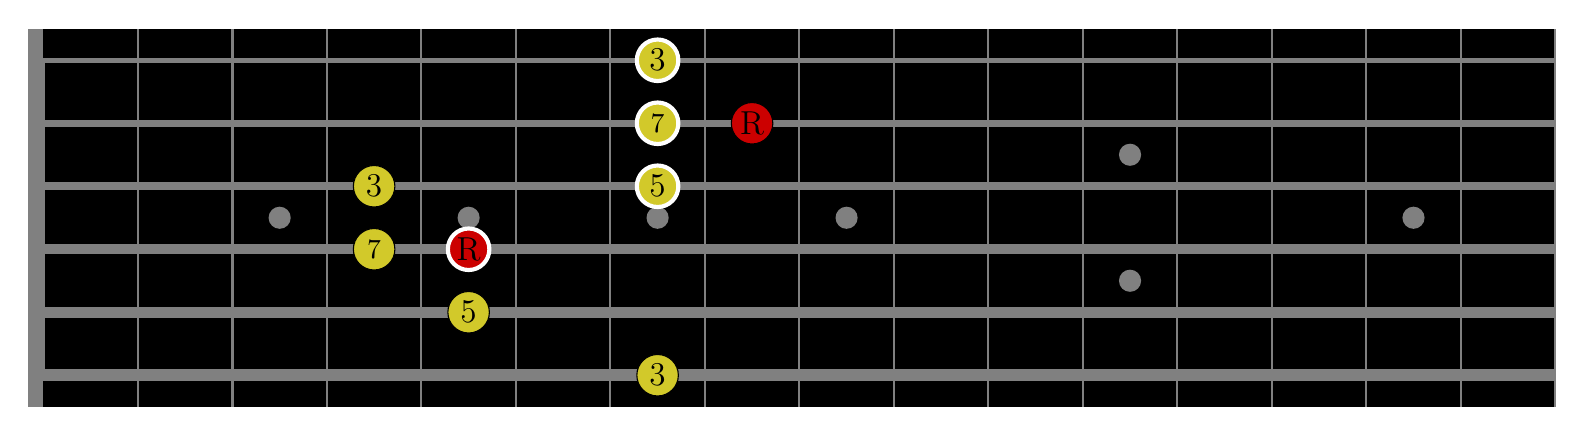
\begin{tikzpicture}[scale=1]
	\def \h{0.8}
	\def \fret{1.2} % 1.6
	\def \L{ 16*\fret }	
	\def \dot_size{4pt}
	\def \circ_size{15pt}
	
	\fill[black, line width=2] (0.0,-0.4) rectangle (16*\fret,4.4);
	\fill[black!50!white, line width=2] (-0.2,-0.4) rectangle (0,4.4);
	
	% Strings
	\draw[color=black!50!white, line width=2.0]  (-0.1, 5*\h) -- (\L,5*\h); % E
	\draw[color=black!50!white, line width=2.5]  (-0.1, 4*\h) -- (\L,4*\h); % B
	\draw[color=black!50!white, line width=3.0]  (-0.1, 3*\h) -- (\L,3*\h); % G
	\draw[color=black!50!white, line width=3.5]  (-0.1, 2*\h) -- (\L,2*\h); % D
	\draw[color=black!50!white, line width=4.0]  (-0.1, 1*\h) -- (\L,1*\h); % A
	\draw[color=black!50!white, line width=4.5]  (-0.1, 0*\h) -- (\L,0*\h); % E
	
	% Frets 0
	\draw[color=black!50!white, thick]  (-0.1, 0) -- (-0.1,5*\h); 
	\draw[color=black!50!white, thick]  (0, 0)   -- (0,5*\h); 
	
	% Fret 1-15
	\draw[color=black!50!white, thick]  (\fret,   -0.4)   -- (\fret,4.4);   
	\draw[color=black!50!white, thick]  (2*\fret, -0.4) -- (2*\fret,4.4); 
	\draw[color=black!50!white, thick]  (3*\fret, -0.4) -- (3*\fret,4.4); 
	\draw[color=black!50!white, thick]  (4*\fret, -0.4) -- (4*\fret,4.4); 
	\draw[color=black!50!white, thick]  (5*\fret, -0.4) -- (5*\fret,4.4); 
	\draw[color=black!50!white, thick]  (6*\fret, -0.4) -- (6*\fret,4.4); 
	\draw[color=black!50!white, thick]  (7*\fret, -0.4) -- (7*\fret,4.4); 
	\draw[color=black!50!white, thick]  (8*\fret, -0.4) -- (8*\fret,4.4); 
	\draw[color=black!50!white, thick]  (9*\fret, -0.4) -- (9*\fret,4.4); 
	\draw[color=black!50!white, thick]  (10*\fret, -0.4) -- (10*\fret,4.4); 
	\draw[color=black!50!white, thick]  (11*\fret, -0.4) -- (11*\fret,4.4); 
	\draw[color=black!50!white, thick]  (12*\fret, -0.4) -- (12*\fret,4.4); 
	\draw[color=black!50!white, thick]  (13*\fret, -0.4) -- (13*\fret,4.4); 
	\draw[color=black!50!white, thick]  (14*\fret, -0.4) -- (14*\fret,4.4); 
	\draw[color=black!50!white, thick]  (15*\fret, -0.4) -- (15*\fret,4.4); 
	\draw[color=black!50!white, thick]  (16*\fret, -0.4) -- (16*\fret,4.4); 
	%\draw[color=black!50!white, thick]  (17*\fret, -0.4) -- (17*\fret,4.4); 
	%\draw[color=black!50!white, thick]  (18*\fret, -0.4) -- (18*\fret,4.4); 
	%\draw[color=black!50!white, thick]  (19*\fret, -0.4) -- (19*\fret,4.4); 
	%\draw[color=black!50!white, thick]  (20*\fret, -0.4) -- (20*\fret,4.4); 
	
	% Dots
	\fill[black!50!white] (2.5*\fret,2.5*\h) circle (\dot_size); % fret 3
	\fill[black!50!white] (4.5*\fret,2.5*\h) circle (\dot_size); % fret 5
	\fill[black!50!white] (6.5*\fret,2.5*\h) circle (\dot_size); % fret 7
	\fill[black!50!white] (8.5*\fret,2.5*\h) circle (\dot_size); % fret 9
	\fill[black!50!white] (11.5*\fret,1.5*\h) circle (\dot_size); % fret 12
	\fill[black!50!white] (11.5*\fret,3.5*\h) circle (\dot_size); % fret 12
	\fill[black!50!white] (14.5*\fret,2.5*\h) circle (\dot_size); % fret 15
	%\fill[black!50!white] (16.5*\fret,2.5*\h) circle (\dot_size); % fret 17
	%\fill[black!50!white] (18.5*\fret,2.5*\h) circle (\dot_size); % fret 19

	
	% Arpege (position E)
	\node[dot=\circ_size, fill=yellow!80!black,draw] at (6.5*\fret,0*\h) {{\large 3}};
	\node[dot=\circ_size, fill=yellow!80!black,draw] at (4.5*\fret,1*\h) {{\large 5}};
	\node[dot=\circ_size, fill=yellow!80!black,draw] at (3.5*\fret,2*\h) {{\normalsize 7}};
	\node[dot=\circ_size, fill=red!80!black,draw=white, line width=1.5pt] at (4.5*\fret,2*\h) {{\large R}};
	\node[dot=\circ_size, fill=yellow!80!black,draw] at (3.5*\fret,3*\h) {{\large 3}};
	\node[dot=\circ_size, fill=yellow!80!black, draw=white, line width=1.5pt] at (6.5*\fret,3*\h) {{\large 5}};
	\node[dot=\circ_size, fill=yellow!80!black,  draw=white, line width=1.5pt] at (6.5*\fret,4*\h) {{\normalsize 7}};
	\node[dot=\circ_size, fill=red!80!black ,draw] at (7.5*\fret,4*\h) {{\large R}};
	\node[dot=\circ_size, fill=yellow!80!black ,draw=white, line width=1.5pt] at (6.5*\fret,5*\h) {{\large 3}};
	
	% Arpege (position A)
%	\node[dot=\circ_size, fill=yellow!50!red!80!white,draw] at (13.5*\fret,1*\h) {{\large 3}};
%	\node[dot=\circ_size, fill=yellow!50!red!80!white,draw] at (11.5*\fret,2*\h) {{\large 5}};
%	\node[dot=\circ_size, fill=white,draw] at (10.5*\fret,3*\h) {{\normalsize 7}};
%	\node[dot=\circ_size, fill=yellow!50!red!80!white,draw] at (11.5*\fret,3*\h) {{\large R}};
%	\node[dot=\circ_size, fill=yellow!50!red!80!white,draw] at (11.5*\fret,4*\h) {{\large 3}};
%	\node[dot=\circ_size, fill=white,draw] at (13.5*\fret,5*\h) {{\normalsize 7}};
%	\node[dot=\circ_size, fill=yellow!50!red!80!white,draw] at (14.5*\fret,5*\h) {{\large R}};

%	% Annotation
%	\draw[black,anchor=west] (-3cm,2cm) node { {\Huge $\Delta$7 } };
	
\end{tikzpicture}
%\end{document}




}
	\hspace*{-0cm}
	\scalebox{0.52}{%\documentclass{standalone}
%\usepackage{pgfplots} % Include package for TikZ and PGF plot
%\usepackage{anyfontsize} % enable to change the font size manually
%\usepackage{makecell}%
%\usetikzlibrary{shapes.geometric}
%\tikzset{
%dot/.style = {circle, fill, minimum size=#1,
%              inner sep=0pt, outer sep=0pt},
%dot/.default = 6pt % size of the circle diameter
%}
% \renewcommand{\familydefault}{\sfdefault}

%\begin{document}
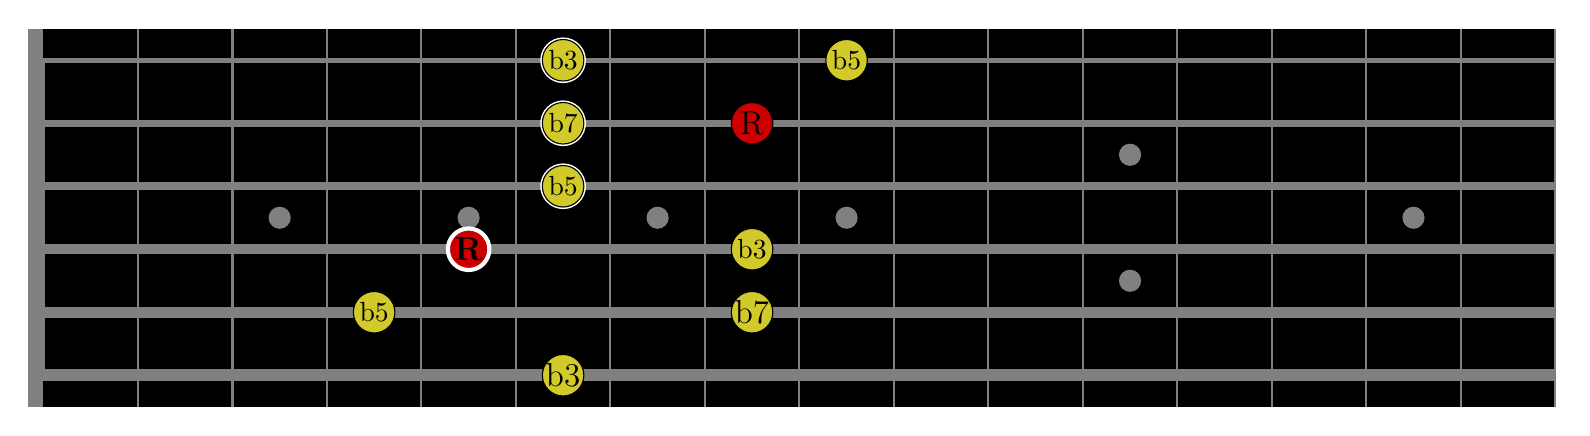
\begin{tikzpicture}[scale=1]
	\def \h{0.8}
	\def \fret{1.2} % 1.6
	\def \L{ 16*\fret }	
	\def \dot_size{4pt}
	\def \circ_size{15pt}
	
	\fill[black, line width=2] (0.0,-0.4) rectangle (16*\fret,4.4);
	\fill[black!50!white, line width=2] (-0.2,-0.4) rectangle (0,4.4);
	
	% Strings
	\draw[color=black!50!white, line width=2.0]  (-0.1, 5*\h) -- (\L,5*\h); % E
	\draw[color=black!50!white, line width=2.5]  (-0.1, 4*\h) -- (\L,4*\h); % B
	\draw[color=black!50!white, line width=3.0]  (-0.1, 3*\h) -- (\L,3*\h); % G
	\draw[color=black!50!white, line width=3.5]  (-0.1, 2*\h) -- (\L,2*\h); % D
	\draw[color=black!50!white, line width=4.0]  (-0.1, 1*\h) -- (\L,1*\h); % A
	\draw[color=black!50!white, line width=4.5]  (-0.1, 0*\h) -- (\L,0*\h); % E
	
	% Frets 0
	\draw[color=black!50!white, thick]  (-0.1, 0) -- (-0.1,5*\h); 
	\draw[color=black!50!white, thick]  (0, 0)   -- (0,5*\h); 
	
	% Fret 1-15
	\draw[color=black!50!white, thick]  (\fret,   -0.4)   -- (\fret,4.4);   
	\draw[color=black!50!white, thick]  (2*\fret, -0.4) -- (2*\fret,4.4); 
	\draw[color=black!50!white, thick]  (3*\fret, -0.4) -- (3*\fret,4.4); 
	\draw[color=black!50!white, thick]  (4*\fret, -0.4) -- (4*\fret,4.4); 
	\draw[color=black!50!white, thick]  (5*\fret, -0.4) -- (5*\fret,4.4); 
	\draw[color=black!50!white, thick]  (6*\fret, -0.4) -- (6*\fret,4.4); 
	\draw[color=black!50!white, thick]  (7*\fret, -0.4) -- (7*\fret,4.4); 
	\draw[color=black!50!white, thick]  (8*\fret, -0.4) -- (8*\fret,4.4); 
	\draw[color=black!50!white, thick]  (9*\fret, -0.4) -- (9*\fret,4.4); 
	\draw[color=black!50!white, thick]  (10*\fret, -0.4) -- (10*\fret,4.4); 
	\draw[color=black!50!white, thick]  (11*\fret, -0.4) -- (11*\fret,4.4); 
	\draw[color=black!50!white, thick]  (12*\fret, -0.4) -- (12*\fret,4.4); 
	\draw[color=black!50!white, thick]  (13*\fret, -0.4) -- (13*\fret,4.4); 
	\draw[color=black!50!white, thick]  (14*\fret, -0.4) -- (14*\fret,4.4); 
	\draw[color=black!50!white, thick]  (15*\fret, -0.4) -- (15*\fret,4.4); 
	\draw[color=black!50!white, thick]  (16*\fret, -0.4) -- (16*\fret,4.4); 
	%\draw[color=black!50!white, thick]  (17*\fret, -0.4) -- (17*\fret,4.4); 
	%\draw[color=black!50!white, thick]  (18*\fret, -0.4) -- (18*\fret,4.4); 
	%\draw[color=black!50!white, thick]  (19*\fret, -0.4) -- (19*\fret,4.4); 
	%\draw[color=black!50!white, thick]  (20*\fret, -0.4) -- (20*\fret,4.4); 
	
	% Dots
	\fill[black!50!white] (2.5*\fret,2.5*\h) circle (\dot_size); % fret 3
	\fill[black!50!white] (4.5*\fret,2.5*\h) circle (\dot_size); % fret 5
	\fill[black!50!white] (6.5*\fret,2.5*\h) circle (\dot_size); % fret 7
	\fill[black!50!white] (8.5*\fret,2.5*\h) circle (\dot_size); % fret 9
	\fill[black!50!white] (11.5*\fret,1.5*\h) circle (\dot_size); % fret 12
	\fill[black!50!white] (11.5*\fret,3.5*\h) circle (\dot_size); % fret 12
	\fill[black!50!white] (14.5*\fret,2.5*\h) circle (\dot_size); % fret 15
	%\fill[black!50!white] (16.5*\fret,2.5*\h) circle (\dot_size); % fret 17
	%\fill[black!50!white] (18.5*\fret,2.5*\h) circle (\dot_size); % fret 19

	
	% Arpege (position A)
	\node[dot=\circ_size, fill=yellow!80!black,draw] at (5.5*\fret,0) {{\large b3}};
	\node[dot=\circ_size, fill=yellow!80!black,draw] at (3.5*\fret,1*\h) {{\normalsize b5}};
	\node[dot=\circ_size, fill=yellow!80!black,draw] at (7.5*\fret,1*\h) {{\large b7}};
	\node[dot=\circ_size, fill=red!80!black,draw=white, line width=1.5pt] at (4.5*\fret,2*\h) {{\large \textbf{R}}};
	\node[dot=\circ_size, fill=yellow!80!black,draw] at (7.5*\fret,2*\h) {{\normalsize b3}};
	\node[dot=\circ_size, fill=yellow!80!black,draw=white, line width=1.5pt] at (5.5*\fret,3*\h) {{\normalsize b5}};
	\node[dot=\circ_size, fill=yellow!80!black,draw] at (5.5*\fret,3*\h) {{\normalsize b5}};
	\node[dot=\circ_size, fill=yellow!80!black,draw=white, line width=1.5pt] at (5.5*\fret,4*\h) {{\large b7}};
	\node[dot=\circ_size, fill=red!80!black,draw] at (7.5*\fret,4*\h) {{\large R}};
	\node[dot=\circ_size, fill=yellow!80!black,draw] at (5.5*\fret,4*\h) {{\normalsize b7}};
	\node[dot=\circ_size, fill=yellow!80!black,draw=white, line width=1.5pt] at (5.5*\fret,5*\h) {{\normalsize b3}};
	\node[dot=\circ_size, fill=yellow!80!black,draw] at (5.5*\fret,5*\h) {{\normalsize b3}};
	\node[dot=\circ_size, fill=yellow!80!black,draw] at (8.5*\fret,5*\h) {{\normalsize b5}};
%
%	% Arpege (position D-C)
%	\node[dot=\circ_size, fill=yellow!50!red!80!white,draw] at (12.5*\fret,1*\h) {{\normalsize b3}};
%	\node[dot=\circ_size, fill=yellow!50!red!80!white,draw] at (10.5*\fret,2*\h) {{\normalsize b5}};
%	\node[dot=\circ_size, fill=white,draw] at (9.5*\fret,3*\h) {{\large 7}};
%	\node[dot=\circ_size, fill=yellow!50!red!80!white,draw] at (11.5*\fret,3*\h) {{\large R}};
%	\node[dot=\circ_size, fill=yellow!50!red!80!white,draw] at (10.5*\fret,4*\h) {{\normalsize b3}};
%	\node[dot=\circ_size, fill=white,draw] at (12.5*\fret,5*\h) {{\large 7}};

%	% Annotation
%	\draw[black,anchor=west] (-3cm,2cm) node { {\Huge b7b5 } };
	
\end{tikzpicture}
%\end{document}




}

	\hspace*{-4.2cm}
	\scalebox{0.52}{
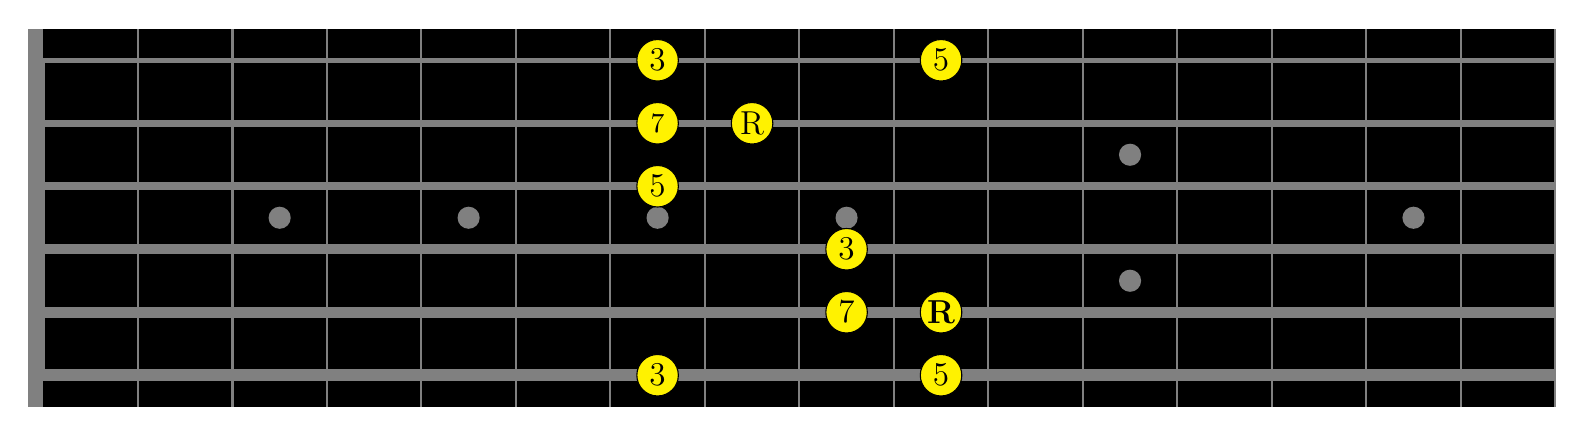
\begin{tikzpicture}[scale=1]
	\def \h{0.8}
	\def \fret{1.2} % 1.6
	\def \L{ 16*\fret }	
	\def \dot_size{4pt}
	\def \circ_size{15pt}
	
	\fill[black, line width=2] (0.0,-0.4) rectangle (16*\fret,4.4);
	\fill[black!50!white, line width=2] (-0.2,-0.4) rectangle (0,4.4);
	
	% Strings
	\draw[color=black!50!white, line width=2.0]  (-0.1, 5*\h) -- (\L,5*\h); % E
	\draw[color=black!50!white, line width=2.5]  (-0.1, 4*\h) -- (\L,4*\h); % B
	\draw[color=black!50!white, line width=3.0]  (-0.1, 3*\h) -- (\L,3*\h); % G
	\draw[color=black!50!white, line width=3.5]  (-0.1, 2*\h) -- (\L,2*\h); % D
	\draw[color=black!50!white, line width=4.0]  (-0.1, 1*\h) -- (\L,1*\h); % A
	\draw[color=black!50!white, line width=4.5]  (-0.1, 0*\h) -- (\L,0*\h); % E
	
	% Frets 0
	\draw[color=black!50!white, thick]  (-0.1, 0) -- (-0.1,5*\h); 
	\draw[color=black!50!white, thick]  (0, 0)   -- (0,5*\h); 
	
	% Fret 1-15
	\draw[color=black!50!white, thick]  (\fret,   -0.4)   -- (\fret,4.4);   
	\draw[color=black!50!white, thick]  (2*\fret, -0.4) -- (2*\fret,4.4); 
	\draw[color=black!50!white, thick]  (3*\fret, -0.4) -- (3*\fret,4.4); 
	\draw[color=black!50!white, thick]  (4*\fret, -0.4) -- (4*\fret,4.4); 
	\draw[color=black!50!white, thick]  (5*\fret, -0.4) -- (5*\fret,4.4); 
	\draw[color=black!50!white, thick]  (6*\fret, -0.4) -- (6*\fret,4.4); 
	\draw[color=black!50!white, thick]  (7*\fret, -0.4) -- (7*\fret,4.4); 
	\draw[color=black!50!white, thick]  (8*\fret, -0.4) -- (8*\fret,4.4); 
	\draw[color=black!50!white, thick]  (9*\fret, -0.4) -- (9*\fret,4.4); 
	\draw[color=black!50!white, thick]  (10*\fret, -0.4) -- (10*\fret,4.4); 
	\draw[color=black!50!white, thick]  (11*\fret, -0.4) -- (11*\fret,4.4); 
	\draw[color=black!50!white, thick]  (12*\fret, -0.4) -- (12*\fret,4.4); 
	\draw[color=black!50!white, thick]  (13*\fret, -0.4) -- (13*\fret,4.4); 
	\draw[color=black!50!white, thick]  (14*\fret, -0.4) -- (14*\fret,4.4); 
	\draw[color=black!50!white, thick]  (15*\fret, -0.4) -- (15*\fret,4.4); 
	\draw[color=black!50!white, thick]  (16*\fret, -0.4) -- (16*\fret,4.4); 
	%\draw[color=black!50!white, thick]  (17*\fret, -0.4) -- (17*\fret,4.4); 
	%\draw[color=black!50!white, thick]  (18*\fret, -0.4) -- (18*\fret,4.4); 
	%\draw[color=black!50!white, thick]  (19*\fret, -0.4) -- (19*\fret,4.4); 
	%\draw[color=black!50!white, thick]  (20*\fret, -0.4) -- (20*\fret,4.4); 
	
	% Dots
	\fill[black!50!white] (2.5*\fret,2.5*\h) circle (\dot_size); % fret 3
	\fill[black!50!white] (4.5*\fret,2.5*\h) circle (\dot_size); % fret 5
	\fill[black!50!white] (6.5*\fret,2.5*\h) circle (\dot_size); % fret 7
	\fill[black!50!white] (8.5*\fret,2.5*\h) circle (\dot_size); % fret 9
	\fill[black!50!white] (11.5*\fret,1.5*\h) circle (\dot_size); % fret 12
	\fill[black!50!white] (11.5*\fret,3.5*\h) circle (\dot_size); % fret 12
	\fill[black!50!white] (14.5*\fret,2.5*\h) circle (\dot_size); % fret 15
	%\fill[black!50!white] (16.5*\fret,2.5*\h) circle (\dot_size); % fret 17
	%\fill[black!50!white] (18.5*\fret,2.5*\h) circle (\dot_size); % fret 19

	
	% Arpege (position E)
	\node[dot=\circ_size, fill=yellow,draw] at (6.5*\fret,0*\h) {{\large 3}};
	\node[dot=\circ_size, fill=yellow,draw] at (9.5*\fret,0*\h) {{\large 5}};
	\node[dot=\circ_size, fill=yellow,draw] at (8.5*\fret,1*\h) {{\large 7}};
	\node[dot=\circ_size, fill=yellow,draw] at (8.5*\fret,2*\h) {{\large 3}};
	\node[dot=\circ_size, fill=yellow,draw] at (9.5*\fret,1*\h) {{\large \textbf{R}}};
	\node[dot=\circ_size, fill=yellow, draw] at (6.5*\fret,3*\h) {{\large 5}};
	\node[dot=\circ_size, fill=yellow,  draw] at (6.5*\fret,4*\h) {{\normalsize 7}};
	\node[dot=\circ_size, fill=yellow ,draw] at (7.5*\fret,4*\h) {{\large R}};
	\node[dot=\circ_size, fill=yellow ,draw] at (6.5*\fret,5*\h) {{\large 3}};
	\node[dot=\circ_size, fill=yellow,draw] at (9.5*\fret,5*\h) {{\large 5}};


%	% Annotation
%	\draw[black,anchor=west] (-3cm,2cm) node { {\Huge $\Delta$7 } };
	
\end{tikzpicture}
%\end{document}




}
	\hspace*{-0cm}
	\scalebox{0.52}{%\documentclass{standalone}
%\usepackage{pgfplots} % Include package for TikZ and PGF plot
%\usepackage{anyfontsize} % enable to change the font size manually
%\usepackage{makecell}%
%\usetikzlibrary{shapes.geometric}
%\tikzset{
%dot/.style = {circle, fill, minimum size=#1,
%              inner sep=0pt, outer sep=0pt},
%dot/.default = 6pt % size of the circle diameter
%}
% \renewcommand{\familydefault}{\sfdefault}

%\begin{document}
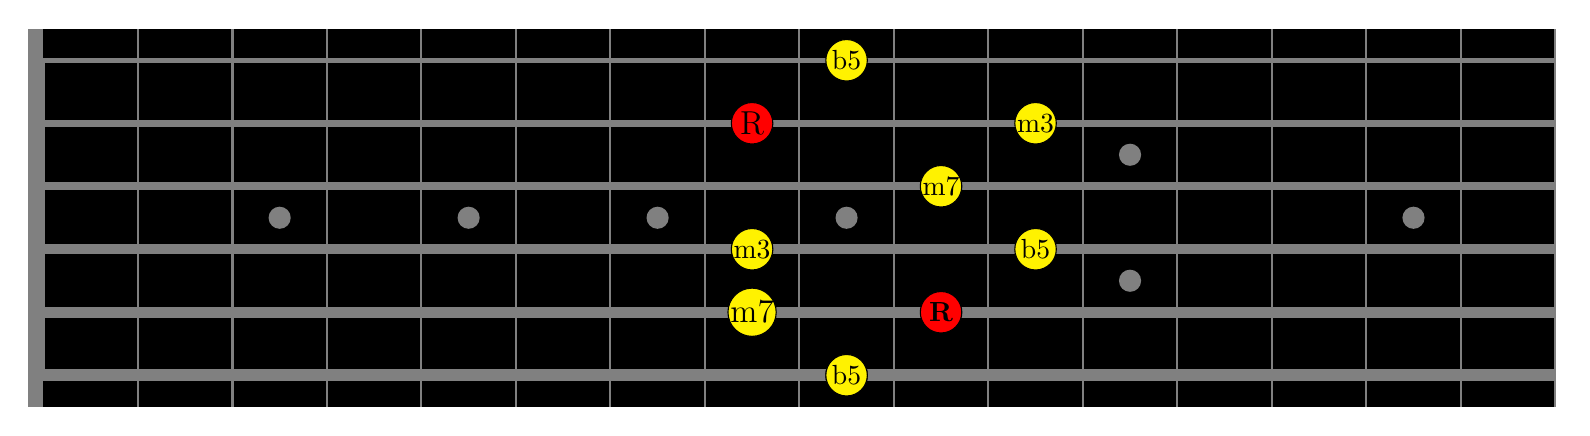
\begin{tikzpicture}[scale=1]
	\def \h{0.8}
	\def \fret{1.2} % 1.6
	\def \L{ 16*\fret }	
	\def \dot_size{4pt}
	\def \circ_size{15pt}
	
	\fill[black, line width=2] (0.0,-0.4) rectangle (16*\fret,4.4);
	\fill[black!50!white, line width=2] (-0.2,-0.4) rectangle (0,4.4);
	
	% Strings
	\draw[color=black!50!white, line width=2.0]  (-0.1, 5*\h) -- (\L,5*\h); % E
	\draw[color=black!50!white, line width=2.5]  (-0.1, 4*\h) -- (\L,4*\h); % B
	\draw[color=black!50!white, line width=3.0]  (-0.1, 3*\h) -- (\L,3*\h); % G
	\draw[color=black!50!white, line width=3.5]  (-0.1, 2*\h) -- (\L,2*\h); % D
	\draw[color=black!50!white, line width=4.0]  (-0.1, 1*\h) -- (\L,1*\h); % A
	\draw[color=black!50!white, line width=4.5]  (-0.1, 0*\h) -- (\L,0*\h); % E
	
	% Frets 0
	\draw[color=black!50!white, thick]  (-0.1, 0) -- (-0.1,5*\h); 
	\draw[color=black!50!white, thick]  (0, 0)   -- (0,5*\h); 
	
	% Fret 1-15
	\draw[color=black!50!white, thick]  (\fret,   -0.4)   -- (\fret,4.4);   
	\draw[color=black!50!white, thick]  (2*\fret, -0.4) -- (2*\fret,4.4); 
	\draw[color=black!50!white, thick]  (3*\fret, -0.4) -- (3*\fret,4.4); 
	\draw[color=black!50!white, thick]  (4*\fret, -0.4) -- (4*\fret,4.4); 
	\draw[color=black!50!white, thick]  (5*\fret, -0.4) -- (5*\fret,4.4); 
	\draw[color=black!50!white, thick]  (6*\fret, -0.4) -- (6*\fret,4.4); 
	\draw[color=black!50!white, thick]  (7*\fret, -0.4) -- (7*\fret,4.4); 
	\draw[color=black!50!white, thick]  (8*\fret, -0.4) -- (8*\fret,4.4); 
	\draw[color=black!50!white, thick]  (9*\fret, -0.4) -- (9*\fret,4.4); 
	\draw[color=black!50!white, thick]  (10*\fret, -0.4) -- (10*\fret,4.4); 
	\draw[color=black!50!white, thick]  (11*\fret, -0.4) -- (11*\fret,4.4); 
	\draw[color=black!50!white, thick]  (12*\fret, -0.4) -- (12*\fret,4.4); 
	\draw[color=black!50!white, thick]  (13*\fret, -0.4) -- (13*\fret,4.4); 
	\draw[color=black!50!white, thick]  (14*\fret, -0.4) -- (14*\fret,4.4); 
	\draw[color=black!50!white, thick]  (15*\fret, -0.4) -- (15*\fret,4.4); 
	\draw[color=black!50!white, thick]  (16*\fret, -0.4) -- (16*\fret,4.4); 
	%\draw[color=black!50!white, thick]  (17*\fret, -0.4) -- (17*\fret,4.4); 
	%\draw[color=black!50!white, thick]  (18*\fret, -0.4) -- (18*\fret,4.4); 
	%\draw[color=black!50!white, thick]  (19*\fret, -0.4) -- (19*\fret,4.4); 
	%\draw[color=black!50!white, thick]  (20*\fret, -0.4) -- (20*\fret,4.4); 
	
	% Dots
	\fill[black!50!white] (2.5*\fret,2.5*\h) circle (\dot_size); % fret 3
	\fill[black!50!white] (4.5*\fret,2.5*\h) circle (\dot_size); % fret 5
	\fill[black!50!white] (6.5*\fret,2.5*\h) circle (\dot_size); % fret 7
	\fill[black!50!white] (8.5*\fret,2.5*\h) circle (\dot_size); % fret 9
	\fill[black!50!white] (11.5*\fret,1.5*\h) circle (\dot_size); % fret 12
	\fill[black!50!white] (11.5*\fret,3.5*\h) circle (\dot_size); % fret 12
	\fill[black!50!white] (14.5*\fret,2.5*\h) circle (\dot_size); % fret 15
	%\fill[black!50!white] (16.5*\fret,2.5*\h) circle (\dot_size); % fret 17
	%\fill[black!50!white] (18.5*\fret,2.5*\h) circle (\dot_size); % fret 19

	
	% Arpege
	\node[dot=\circ_size, fill=yellow,draw] at (8.5*\fret,0*\h) {{\normalsize b5}};
	\node[dot=\circ_size, fill=yellow,draw] at (8.5*\fret,0*\h) {{\normalsize b5}};
	\node[dot=\circ_size, fill=red,draw] at (9.5*\fret,1*\h) {{\normalsize \textbf{R}}};
	\node[dot=\circ_size, fill=yellow,draw] at (7.5*\fret,1*\h) {{\large m7}};
	\node[dot=\circ_size, fill=yellow,draw] at (10.5*\fret,2*\h) {{\normalsize b5}};
	\node[dot=\circ_size, fill=yellow,draw] at (7.5*\fret,2*\h) {{\normalsize m3}};
	\node[dot=\circ_size, fill=yellow,draw] at (10.5*\fret,4*\h) {{\normalsize m3}};
	\node[dot=\circ_size, fill=yellow,draw] at (9.5*\fret,3*\h) {{\normalsize m7}};
	\node[dot=\circ_size, fill=red,draw] at (7.5*\fret,4*\h) {{\large R}};
	\node[dot=\circ_size, fill=yellow,draw] at (8.5*\fret,5*\h) {{\normalsize b5}};

%
%	% Arpege (position D-C)
%	\node[dot=\circ_size, fill=yellow!50!red!80!white,draw] at (12.5*\fret,1*\h) {{\normalsize m3}};
%	\node[dot=\circ_size, fill=yellow!50!red!80!white,draw] at (10.5*\fret,2*\h) {{\normalsize b5}};
%	\node[dot=\circ_size, fill=white,draw] at (9.5*\fret,3*\h) {{\large 7}};
%	\node[dot=\circ_size, fill=yellow!50!red!80!white,draw] at (11.5*\fret,3*\h) {{\large R}};
%	\node[dot=\circ_size, fill=yellow!50!red!80!white,draw] at (10.5*\fret,4*\h) {{\normalsize m3}};
%	\node[dot=\circ_size, fill=white,draw] at (12.5*\fret,5*\h) {{\large 7}};

%	% Annotation
%	\draw[black,anchor=west] (-3cm,2cm) node { {\Huge m7b5 } };
	
\end{tikzpicture}
%\end{document}




}

	\hspace*{-4.2cm}
	\scalebox{0.52}{
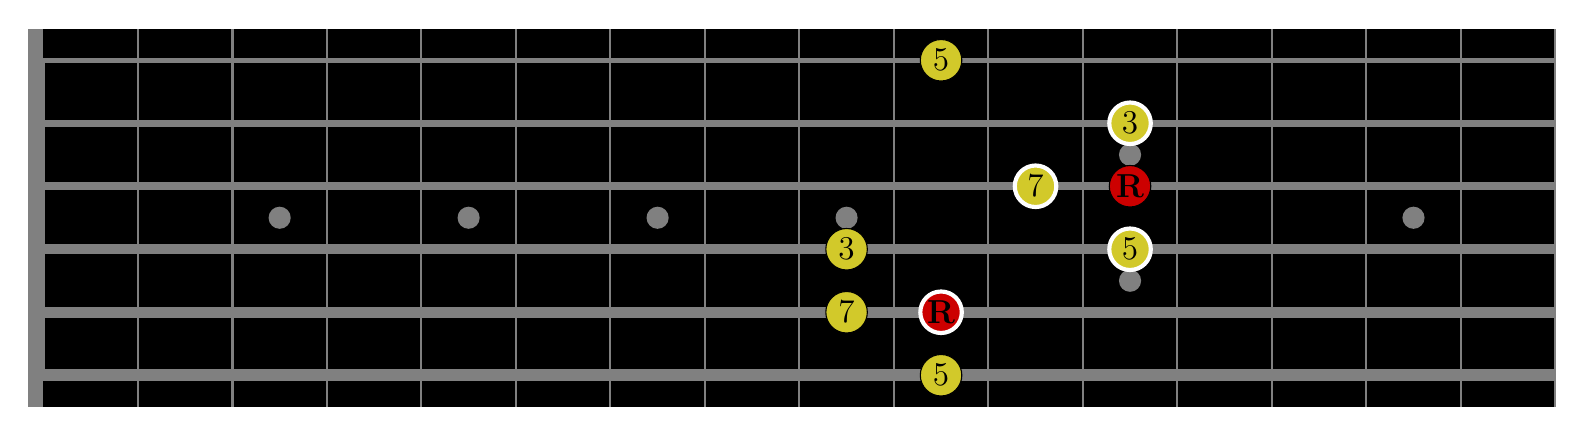
\begin{tikzpicture}[scale=1]
	\def \h{0.8}
	\def \fret{1.2} % 1.6
	\def \L{ 16*\fret }	
	\def \dot_size{4pt}
	\def \circ_size{15pt}
	
	\fill[black, line width=2] (0.0,-0.4) rectangle (16*\fret,4.4);
	\fill[black!50!white, line width=2] (-0.2,-0.4) rectangle (0,4.4);
	
	% Strings
	\draw[color=black!50!white, line width=2.0]  (-0.1, 5*\h) -- (\L,5*\h); % E
	\draw[color=black!50!white, line width=2.5]  (-0.1, 4*\h) -- (\L,4*\h); % B
	\draw[color=black!50!white, line width=3.0]  (-0.1, 3*\h) -- (\L,3*\h); % G
	\draw[color=black!50!white, line width=3.5]  (-0.1, 2*\h) -- (\L,2*\h); % D
	\draw[color=black!50!white, line width=4.0]  (-0.1, 1*\h) -- (\L,1*\h); % A
	\draw[color=black!50!white, line width=4.5]  (-0.1, 0*\h) -- (\L,0*\h); % E
	
	% Frets 0
	\draw[color=black!50!white, thick]  (-0.1, 0) -- (-0.1,5*\h); 
	\draw[color=black!50!white, thick]  (0, 0)   -- (0,5*\h); 
	
	% Fret 1-15
	\draw[color=black!50!white, thick]  (\fret,   -0.4)   -- (\fret,4.4);   
	\draw[color=black!50!white, thick]  (2*\fret, -0.4) -- (2*\fret,4.4); 
	\draw[color=black!50!white, thick]  (3*\fret, -0.4) -- (3*\fret,4.4); 
	\draw[color=black!50!white, thick]  (4*\fret, -0.4) -- (4*\fret,4.4); 
	\draw[color=black!50!white, thick]  (5*\fret, -0.4) -- (5*\fret,4.4); 
	\draw[color=black!50!white, thick]  (6*\fret, -0.4) -- (6*\fret,4.4); 
	\draw[color=black!50!white, thick]  (7*\fret, -0.4) -- (7*\fret,4.4); 
	\draw[color=black!50!white, thick]  (8*\fret, -0.4) -- (8*\fret,4.4); 
	\draw[color=black!50!white, thick]  (9*\fret, -0.4) -- (9*\fret,4.4); 
	\draw[color=black!50!white, thick]  (10*\fret, -0.4) -- (10*\fret,4.4); 
	\draw[color=black!50!white, thick]  (11*\fret, -0.4) -- (11*\fret,4.4); 
	\draw[color=black!50!white, thick]  (12*\fret, -0.4) -- (12*\fret,4.4); 
	\draw[color=black!50!white, thick]  (13*\fret, -0.4) -- (13*\fret,4.4); 
	\draw[color=black!50!white, thick]  (14*\fret, -0.4) -- (14*\fret,4.4); 
	\draw[color=black!50!white, thick]  (15*\fret, -0.4) -- (15*\fret,4.4); 
	\draw[color=black!50!white, thick]  (16*\fret, -0.4) -- (16*\fret,4.4); 
	%\draw[color=black!50!white, thick]  (17*\fret, -0.4) -- (17*\fret,4.4); 
	%\draw[color=black!50!white, thick]  (18*\fret, -0.4) -- (18*\fret,4.4); 
	%\draw[color=black!50!white, thick]  (19*\fret, -0.4) -- (19*\fret,4.4); 
	%\draw[color=black!50!white, thick]  (20*\fret, -0.4) -- (20*\fret,4.4); 
	
	% Dots
	\fill[black!50!white] (2.5*\fret,2.5*\h) circle (\dot_size); % fret 3
	\fill[black!50!white] (4.5*\fret,2.5*\h) circle (\dot_size); % fret 5
	\fill[black!50!white] (6.5*\fret,2.5*\h) circle (\dot_size); % fret 7
	\fill[black!50!white] (8.5*\fret,2.5*\h) circle (\dot_size); % fret 9
	\fill[black!50!white] (11.5*\fret,1.5*\h) circle (\dot_size); % fret 12
	\fill[black!50!white] (11.5*\fret,3.5*\h) circle (\dot_size); % fret 12
	\fill[black!50!white] (14.5*\fret,2.5*\h) circle (\dot_size); % fret 15
	%\fill[black!50!white] (16.5*\fret,2.5*\h) circle (\dot_size); % fret 17
	%\fill[black!50!white] (18.5*\fret,2.5*\h) circle (\dot_size); % fret 19

	
	% Arpege
	\node[dot=\circ_size, fill=yellow!80!black,draw] at (9.5*\fret,0*\h) {{\large 5}};
	\node[dot=\circ_size, fill=yellow!80!black,draw] at (8.5*\fret,1*\h) {{\large 7}};
	\node[dot=\circ_size, fill=red!80!black,draw=white, line width=1.5pt] at (9.5*\fret,1*\h) {{\large \textbf{R}}};
	\node[dot=\circ_size, fill=yellow!80!black,draw=white, line width=1.5pt] at (11.5*\fret,2*\h) {{\large 5}};
	\node[dot=\circ_size, fill=yellow!80!black,draw] at (8.5*\fret,2*\h) {{\large 3}};
	\node[dot=\circ_size, fill=red!80!black,draw] at (11.5*\fret,3*\h) {{\large \textbf{R}}};
	\node[dot=\circ_size, fill=yellow!80!black,draw=white, line width=1.5pt] at (10.5*\fret,3*\h) {{\large 7}};
	\node[dot=\circ_size, fill=yellow!80!black,draw=white, line width=1.5pt] at (11.5*\fret,4*\h) {{\large 3}};
	\node[dot=\circ_size, fill=yellow!80!black,draw] at (9.5*\fret,5*\h) {{\large 5}};


%	% Annotation
%	\draw[black,anchor=west] (-3cm,2cm) node { {\Huge $\Delta$7 } };
	
\end{tikzpicture}
%\end{document}




}
	\hspace*{-0cm}
	\scalebox{0.52}{%\documentclass{standalone}
%\usepackage{pgfplots} % Include package for TikZ and PGF plot
%\usepackage{anyfontsize} % enable to change the font size manually
%\usepackage{makecell}%
%\usetikzlibrary{shapes.geometric}
%\tikzset{
%dot/.style = {circle, fill, minimum size=#1,
%              inner sep=0pt, outer sep=0pt},
%dot/.default = 6pt % size of the circle diameter
%}
% \renewcommand{\familydefault}{\sfdefault}

%\begin{document}
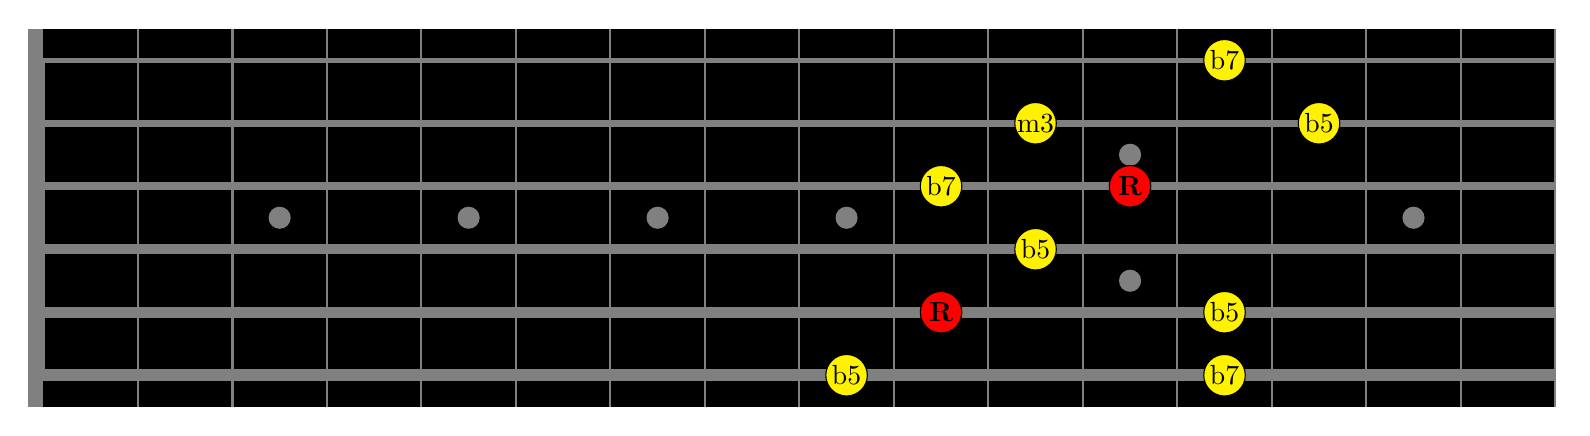
\begin{tikzpicture}[scale=1]
	\def \h{0.8}
	\def \fret{1.2} % 1.6
	\def \L{ 16*\fret }	
	\def \dot_size{4pt}
	\def \circ_size{15pt}
	
	\fill[black, line width=2] (0.0,-0.4) rectangle (16*\fret,4.4);
	\fill[black!50!white, line width=2] (-0.2,-0.4) rectangle (0,4.4);
	
	% Strings
	\draw[color=black!50!white, line width=2.0]  (-0.1, 5*\h) -- (\L,5*\h); % E
	\draw[color=black!50!white, line width=2.5]  (-0.1, 4*\h) -- (\L,4*\h); % B
	\draw[color=black!50!white, line width=3.0]  (-0.1, 3*\h) -- (\L,3*\h); % G
	\draw[color=black!50!white, line width=3.5]  (-0.1, 2*\h) -- (\L,2*\h); % D
	\draw[color=black!50!white, line width=4.0]  (-0.1, 1*\h) -- (\L,1*\h); % A
	\draw[color=black!50!white, line width=4.5]  (-0.1, 0*\h) -- (\L,0*\h); % E
	
	% Frets 0
	\draw[color=black!50!white, thick]  (-0.1, 0) -- (-0.1,5*\h); 
	\draw[color=black!50!white, thick]  (0, 0)   -- (0,5*\h); 
	
	% Fret 1-15
	\draw[color=black!50!white, thick]  (\fret,   -0.4)   -- (\fret,4.4);   
	\draw[color=black!50!white, thick]  (2*\fret, -0.4) -- (2*\fret,4.4); 
	\draw[color=black!50!white, thick]  (3*\fret, -0.4) -- (3*\fret,4.4); 
	\draw[color=black!50!white, thick]  (4*\fret, -0.4) -- (4*\fret,4.4); 
	\draw[color=black!50!white, thick]  (5*\fret, -0.4) -- (5*\fret,4.4); 
	\draw[color=black!50!white, thick]  (6*\fret, -0.4) -- (6*\fret,4.4); 
	\draw[color=black!50!white, thick]  (7*\fret, -0.4) -- (7*\fret,4.4); 
	\draw[color=black!50!white, thick]  (8*\fret, -0.4) -- (8*\fret,4.4); 
	\draw[color=black!50!white, thick]  (9*\fret, -0.4) -- (9*\fret,4.4); 
	\draw[color=black!50!white, thick]  (10*\fret, -0.4) -- (10*\fret,4.4); 
	\draw[color=black!50!white, thick]  (11*\fret, -0.4) -- (11*\fret,4.4); 
	\draw[color=black!50!white, thick]  (12*\fret, -0.4) -- (12*\fret,4.4); 
	\draw[color=black!50!white, thick]  (13*\fret, -0.4) -- (13*\fret,4.4); 
	\draw[color=black!50!white, thick]  (14*\fret, -0.4) -- (14*\fret,4.4); 
	\draw[color=black!50!white, thick]  (15*\fret, -0.4) -- (15*\fret,4.4); 
	\draw[color=black!50!white, thick]  (16*\fret, -0.4) -- (16*\fret,4.4); 
	%\draw[color=black!50!white, thick]  (17*\fret, -0.4) -- (17*\fret,4.4); 
	%\draw[color=black!50!white, thick]  (18*\fret, -0.4) -- (18*\fret,4.4); 
	%\draw[color=black!50!white, thick]  (19*\fret, -0.4) -- (19*\fret,4.4); 
	%\draw[color=black!50!white, thick]  (20*\fret, -0.4) -- (20*\fret,4.4); 
	
	% Dots
	\fill[black!50!white] (2.5*\fret,2.5*\h) circle (\dot_size); % fret 3
	\fill[black!50!white] (4.5*\fret,2.5*\h) circle (\dot_size); % fret 5
	\fill[black!50!white] (6.5*\fret,2.5*\h) circle (\dot_size); % fret 7
	\fill[black!50!white] (8.5*\fret,2.5*\h) circle (\dot_size); % fret 9
	\fill[black!50!white] (11.5*\fret,1.5*\h) circle (\dot_size); % fret 12
	\fill[black!50!white] (11.5*\fret,3.5*\h) circle (\dot_size); % fret 12
	\fill[black!50!white] (14.5*\fret,2.5*\h) circle (\dot_size); % fret 15
	%\fill[black!50!white] (16.5*\fret,2.5*\h) circle (\dot_size); % fret 17
	%\fill[black!50!white] (18.5*\fret,2.5*\h) circle (\dot_size); % fret 19

	% Arpege
	\node[dot=\circ_size, fill=yellow,draw] at (8.5*\fret,0*\h) {{\normalsize b5}};
	\node[dot=\circ_size, fill=yellow,draw] at (12.5*\fret,0*\h) {{\normalsize b7}};
	\node[dot=\circ_size, fill=yellow,draw] at (12.5*\fret,1*\h) {{\normalsize b5}};
	\node[dot=\circ_size, fill=red,draw] at (9.5*\fret,1*\h) {{\normalsize \textbf{R}}};
	\node[dot=\circ_size, fill=yellow,draw] at (10.5*\fret,2*\h) {{\normalsize b5}};
	\node[dot=\circ_size, fill=red,draw] at (11.5*\fret,3*\h) {{\normalsize \textbf{R}}};
	\node[dot=\circ_size, fill=yellow,draw] at (9.5*\fret,3*\h) {{\normalsize b7}};
	\node[dot=\circ_size, fill=yellow,draw] at (10.5*\fret,4*\h) {{\normalsize m3}};
	\node[dot=\circ_size, fill=yellow,draw] at (12.5*\fret,5*\h) {{\normalsize b7}};
	\node[dot=\circ_size, fill=yellow,draw] at (13.5*\fret,4*\h) {{\normalsize b5}};

%	% Annotation
%	\draw[black,anchor=west] (-3cm,2cm) node { {\Huge m7b5 } };
	
\end{tikzpicture}
%\end{document}




}

	\hspace*{-4.2cm}
	\scalebox{0.52}{
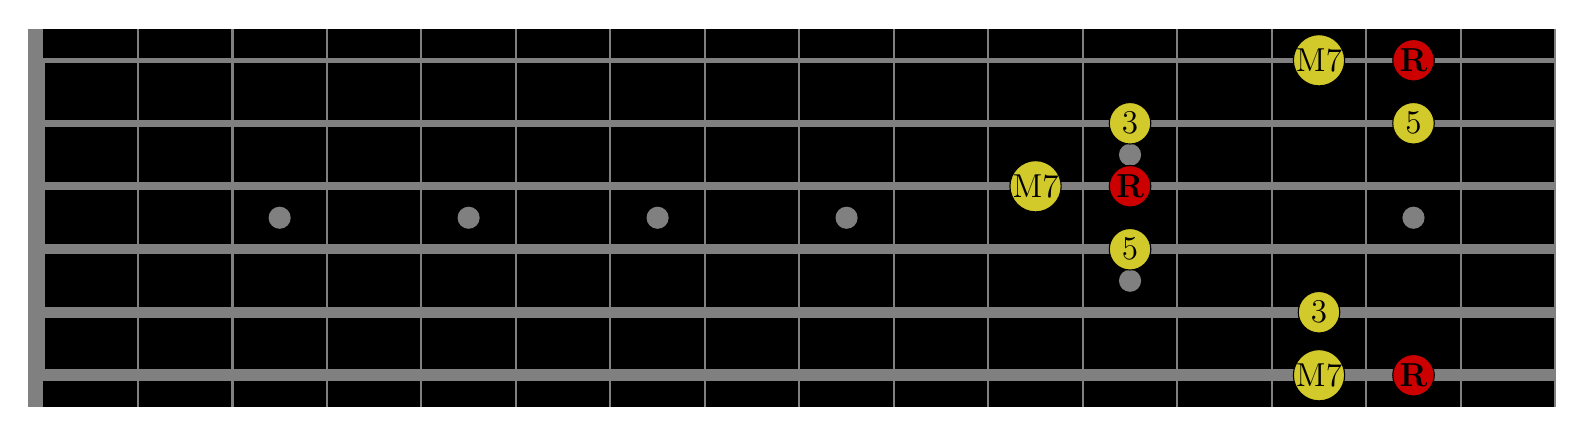
\begin{tikzpicture}[scale=1]
	\def \h{0.8}
	\def \fret{1.2} % 1.6
	\def \L{ 16*\fret }	
	\def \dot_size{4pt}
	\def \circ_size{15pt}
	
	\fill[black, line width=2] (0.0,-0.4) rectangle (16*\fret,4.4);
	\fill[black!50!white, line width=2] (-0.2,-0.4) rectangle (0,4.4);
	
	% Strings
	\draw[color=black!50!white, line width=2.0]  (-0.1, 5*\h) -- (\L,5*\h); % E
	\draw[color=black!50!white, line width=2.5]  (-0.1, 4*\h) -- (\L,4*\h); % B
	\draw[color=black!50!white, line width=3.0]  (-0.1, 3*\h) -- (\L,3*\h); % G
	\draw[color=black!50!white, line width=3.5]  (-0.1, 2*\h) -- (\L,2*\h); % D
	\draw[color=black!50!white, line width=4.0]  (-0.1, 1*\h) -- (\L,1*\h); % A
	\draw[color=black!50!white, line width=4.5]  (-0.1, 0*\h) -- (\L,0*\h); % E
	
	% Frets 0
	\draw[color=black!50!white, thick]  (-0.1, 0) -- (-0.1,5*\h); 
	\draw[color=black!50!white, thick]  (0, 0)   -- (0,5*\h); 
	
	% Fret 1-15
	\draw[color=black!50!white, thick]  (\fret,   -0.4)   -- (\fret,4.4);   
	\draw[color=black!50!white, thick]  (2*\fret, -0.4) -- (2*\fret,4.4); 
	\draw[color=black!50!white, thick]  (3*\fret, -0.4) -- (3*\fret,4.4); 
	\draw[color=black!50!white, thick]  (4*\fret, -0.4) -- (4*\fret,4.4); 
	\draw[color=black!50!white, thick]  (5*\fret, -0.4) -- (5*\fret,4.4); 
	\draw[color=black!50!white, thick]  (6*\fret, -0.4) -- (6*\fret,4.4); 
	\draw[color=black!50!white, thick]  (7*\fret, -0.4) -- (7*\fret,4.4); 
	\draw[color=black!50!white, thick]  (8*\fret, -0.4) -- (8*\fret,4.4); 
	\draw[color=black!50!white, thick]  (9*\fret, -0.4) -- (9*\fret,4.4); 
	\draw[color=black!50!white, thick]  (10*\fret, -0.4) -- (10*\fret,4.4); 
	\draw[color=black!50!white, thick]  (11*\fret, -0.4) -- (11*\fret,4.4); 
	\draw[color=black!50!white, thick]  (12*\fret, -0.4) -- (12*\fret,4.4); 
	\draw[color=black!50!white, thick]  (13*\fret, -0.4) -- (13*\fret,4.4); 
	\draw[color=black!50!white, thick]  (14*\fret, -0.4) -- (14*\fret,4.4); 
	\draw[color=black!50!white, thick]  (15*\fret, -0.4) -- (15*\fret,4.4); 
	\draw[color=black!50!white, thick]  (16*\fret, -0.4) -- (16*\fret,4.4); 
	%\draw[color=black!50!white, thick]  (17*\fret, -0.4) -- (17*\fret,4.4); 
	%\draw[color=black!50!white, thick]  (18*\fret, -0.4) -- (18*\fret,4.4); 
	%\draw[color=black!50!white, thick]  (19*\fret, -0.4) -- (19*\fret,4.4); 
	%\draw[color=black!50!white, thick]  (20*\fret, -0.4) -- (20*\fret,4.4); 
	
	% Dots
	\fill[black!50!white] (2.5*\fret,2.5*\h) circle (\dot_size); % fret 3
	\fill[black!50!white] (4.5*\fret,2.5*\h) circle (\dot_size); % fret 5
	\fill[black!50!white] (6.5*\fret,2.5*\h) circle (\dot_size); % fret 7
	\fill[black!50!white] (8.5*\fret,2.5*\h) circle (\dot_size); % fret 9
	\fill[black!50!white] (11.5*\fret,1.5*\h) circle (\dot_size); % fret 12
	\fill[black!50!white] (11.5*\fret,3.5*\h) circle (\dot_size); % fret 12
	\fill[black!50!white] (14.5*\fret,2.5*\h) circle (\dot_size); % fret 15
	%\fill[black!50!white] (16.5*\fret,2.5*\h) circle (\dot_size); % fret 17
	%\fill[black!50!white] (18.5*\fret,2.5*\h) circle (\dot_size); % fret 19

	
	% Arpege
	\node[dot=\circ_size, fill=red!80!black,draw] at (14.5*\fret,0*\h) {{\large \textbf{R}}};
	\node[dot=\circ_size, fill=yellow!80!black,draw] at (13.5*\fret,0*\h) {{\large M7}};
	\node[dot=\circ_size, fill=yellow!80!black,draw] at (13.5*\fret,1*\h) {{\large 3}};
	\node[dot=\circ_size, fill=yellow!80!black,draw] at (11.5*\fret,2*\h) {{\large 5}};
	\node[dot=\circ_size, fill=red!80!black,draw] at (11.5*\fret,3*\h) {{\large \textbf{R}}};
	\node[dot=\circ_size, fill=yellow!80!black,draw] at (10.5*\fret,3*\h) {{\large M7}};
	\node[dot=\circ_size, fill=yellow!80!black,draw] at (11.5*\fret,4*\h) {{\large 3}};
	\node[dot=\circ_size, fill=yellow!80!black,draw] at (14.5*\fret,4*\h) {{\large 5}};
	\node[dot=\circ_size, fill=yellow!80!black,draw] at (13.5*\fret,5*\h) {{\large M7}};
	\node[dot=\circ_size, fill=red!80!black,draw] at (14.5*\fret,5*\h) {{\large \textbf{R}}};


\end{tikzpicture}




}
	\hspace*{-0cm}
	\scalebox{0.52}{%\documentclass{standalone}
%\usepackage{pgfplots} % Include package for TikZ and PGF plot
%\usepackage{anyfontsize} % enable to change the font size manually
%\usepackage{makecell}%
%\usetikzlibrary{shapes.geometric}
%\tikzset{
%dot/.style = {circle, fill, minimum size=#1,
%              inner sep=0pt, outer sep=0pt},
%dot/.default = 6pt % size of the circle diameter
%}
% \renewcommand{\familydefault}{\sfdefault}

%\begin{document}
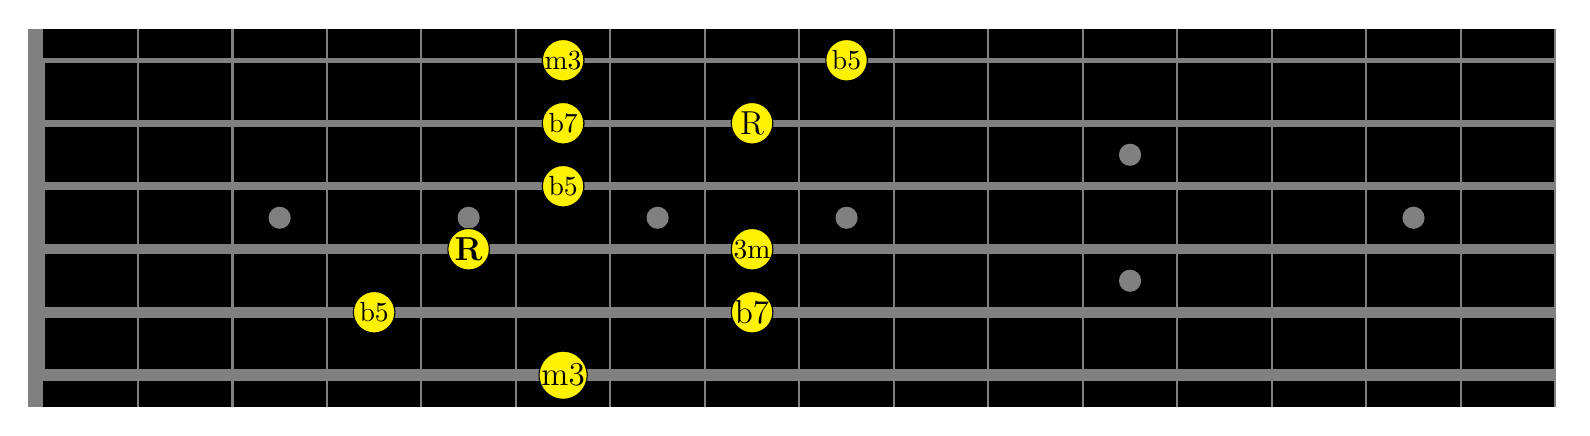
\begin{tikzpicture}[scale=1]
	\def \h{0.8}
	\def \fret{1.2} % 1.6
	\def \L{ 16*\fret }	
	\def \dot_size{4pt}
	\def \circ_size{15pt}
	
	\fill[black, line width=2] (0.0,-0.4) rectangle (16*\fret,4.4);
	\fill[black!50!white, line width=2] (-0.2,-0.4) rectangle (0,4.4);
	
	% Strings
	\draw[color=black!50!white, line width=2.0]  (-0.1, 5*\h) -- (\L,5*\h); % E
	\draw[color=black!50!white, line width=2.5]  (-0.1, 4*\h) -- (\L,4*\h); % B
	\draw[color=black!50!white, line width=3.0]  (-0.1, 3*\h) -- (\L,3*\h); % G
	\draw[color=black!50!white, line width=3.5]  (-0.1, 2*\h) -- (\L,2*\h); % D
	\draw[color=black!50!white, line width=4.0]  (-0.1, 1*\h) -- (\L,1*\h); % A
	\draw[color=black!50!white, line width=4.5]  (-0.1, 0*\h) -- (\L,0*\h); % E
	
	% Frets 0
	\draw[color=black!50!white, thick]  (-0.1, 0) -- (-0.1,5*\h); 
	\draw[color=black!50!white, thick]  (0, 0)   -- (0,5*\h); 
	
	% Fret 1-15
	\draw[color=black!50!white, thick]  (\fret,   -0.4)   -- (\fret,4.4);   
	\draw[color=black!50!white, thick]  (2*\fret, -0.4) -- (2*\fret,4.4); 
	\draw[color=black!50!white, thick]  (3*\fret, -0.4) -- (3*\fret,4.4); 
	\draw[color=black!50!white, thick]  (4*\fret, -0.4) -- (4*\fret,4.4); 
	\draw[color=black!50!white, thick]  (5*\fret, -0.4) -- (5*\fret,4.4); 
	\draw[color=black!50!white, thick]  (6*\fret, -0.4) -- (6*\fret,4.4); 
	\draw[color=black!50!white, thick]  (7*\fret, -0.4) -- (7*\fret,4.4); 
	\draw[color=black!50!white, thick]  (8*\fret, -0.4) -- (8*\fret,4.4); 
	\draw[color=black!50!white, thick]  (9*\fret, -0.4) -- (9*\fret,4.4); 
	\draw[color=black!50!white, thick]  (10*\fret, -0.4) -- (10*\fret,4.4); 
	\draw[color=black!50!white, thick]  (11*\fret, -0.4) -- (11*\fret,4.4); 
	\draw[color=black!50!white, thick]  (12*\fret, -0.4) -- (12*\fret,4.4); 
	\draw[color=black!50!white, thick]  (13*\fret, -0.4) -- (13*\fret,4.4); 
	\draw[color=black!50!white, thick]  (14*\fret, -0.4) -- (14*\fret,4.4); 
	\draw[color=black!50!white, thick]  (15*\fret, -0.4) -- (15*\fret,4.4); 
	\draw[color=black!50!white, thick]  (16*\fret, -0.4) -- (16*\fret,4.4); 
	%\draw[color=black!50!white, thick]  (17*\fret, -0.4) -- (17*\fret,4.4); 
	%\draw[color=black!50!white, thick]  (18*\fret, -0.4) -- (18*\fret,4.4); 
	%\draw[color=black!50!white, thick]  (19*\fret, -0.4) -- (19*\fret,4.4); 
	%\draw[color=black!50!white, thick]  (20*\fret, -0.4) -- (20*\fret,4.4); 
	
	% Dots
	\fill[black!50!white] (2.5*\fret,2.5*\h) circle (\dot_size); % fret 3
	\fill[black!50!white] (4.5*\fret,2.5*\h) circle (\dot_size); % fret 5
	\fill[black!50!white] (6.5*\fret,2.5*\h) circle (\dot_size); % fret 7
	\fill[black!50!white] (8.5*\fret,2.5*\h) circle (\dot_size); % fret 9
	\fill[black!50!white] (11.5*\fret,1.5*\h) circle (\dot_size); % fret 12
	\fill[black!50!white] (11.5*\fret,3.5*\h) circle (\dot_size); % fret 12
	\fill[black!50!white] (14.5*\fret,2.5*\h) circle (\dot_size); % fret 15
	%\fill[black!50!white] (16.5*\fret,2.5*\h) circle (\dot_size); % fret 17
	%\fill[black!50!white] (18.5*\fret,2.5*\h) circle (\dot_size); % fret 19

	
	% Arpege (position A)
	\node[dot=\circ_size, fill=yellow,draw] at (5.5*\fret,0) {{\large m3}};
	\node[dot=\circ_size, fill=yellow,draw] at (3.5*\fret,1*\h) {{\normalsize b5}};
	\node[dot=\circ_size, fill=yellow,draw] at (7.5*\fret,1*\h) {{\large b7}};
	\node[dot=\circ_size, fill=yellow,draw] at (4.5*\fret,2*\h) {{\large \textbf{R}}};
	\node[dot=\circ_size, fill=yellow,draw] at (7.5*\fret,2*\h) {{\normalsize 3m}};
	\node[dot=\circ_size, fill=yellow,draw] at (5.5*\fret,3*\h) {{\normalsize b5}};
	\node[dot=\circ_size, fill=yellow,draw] at (5.5*\fret,3*\h) {{\normalsize b5}};
	\node[dot=\circ_size, fill=yellow,draw] at (5.5*\fret,4*\h) {{\large 7}};
	\node[dot=\circ_size, fill=yellow,draw] at (7.5*\fret,4*\h) {{\large R}};
	\node[dot=\circ_size, fill=yellow,draw] at (5.5*\fret,4*\h) {{\normalsize b7}};
	\node[dot=\circ_size, fill=yellow,draw] at (5.5*\fret,5*\h) {{\normalsize m3}};
	\node[dot=\circ_size, fill=yellow,draw] at (5.5*\fret,5*\h) {{\normalsize m3}};
	\node[dot=\circ_size, fill=yellow,draw] at (8.5*\fret,5*\h) {{\normalsize b5}};
%
%	\node[dot=\circ_size, fill=yellow!50!red!80!white,draw] at (12.5*\fret,1*\h) {{\normalsize m3}};
%	\node[dot=\circ_size, fill=yellow!50!red!80!white,draw] at (10.5*\fret,2*\h) {{\normalsize b5}};
%	\node[dot=\circ_size, fill=white,draw] at (9.5*\fret,3*\h) {{\large 7}};
%	\node[dot=\circ_size, fill=yellow!50!red!80!white,draw] at (11.5*\fret,3*\h) {{\large R}};
%	\node[dot=\circ_size, fill=yellow!50!red!80!white,draw] at (10.5*\fret,4*\h) {{\normalsize m3}};
%	\node[dot=\circ_size, fill=white,draw] at (12.5*\fret,5*\h) {{\large 7}};

%	% Annotation
%	\draw[black,anchor=west] (-3cm,2cm) node { {\Huge m7b5 } };
	
\end{tikzpicture}
%\end{document}




}

	\caption{(left) maj7 arpeggio. (right) m7b5 arpeggio}
	\label{fig:arpeggio}
\end{table}



%%%%%%%%%%%%%%%%%%%%%%%%%%%%%%%%%%%%%%%%%%%%%%%%%%%%%%%%%%%%%%%%%%
\newpage
\section{Modes}

\begin{itemize}
	\item Ionian (Joy), dorian(Jazz), phrygian(flamenco,doom), lydian (floaty,mystery) (ex: E.T., Jurassic Park, Back to the Future), mixo(blues)(ex: AC/DC), aeolian(sad)(ex: Losing my Religion), locrian(tension)(ex:Bjork Army of Me)
\end{itemize}

%%%%%%%%%%%%%%%%%%%%%%%%%%%%%%%%%%%%%%%%%%%%%%%%%%%%%%%%%%%%%%%%%%
\newpage
\section{Transposition}

https://www.youtube.com/watch?v=Vxac3hHrxg8

%%%%%%%%%%%%%%%%%%%%%%%%%%%%%%%%%%%%%%%%%%%%%%%%%%%%%%%%%%%%%%%%%%
\newpage
\section{Composition variation (Shred Master Scott)}

\begin{itemize}
	\item Pedal tone
	\item Inversion
	\item Voice leading
\end{itemize}

%\newpage
%\bibliographystyle{plain}
%\bibliography{/home/jh/Documents/library.bib}

\end{document}
